% !TEX root =  main.tex
\documentclass[12pt]{yalephd}

%\usepackage{times}
\usepackage{epigraph}
\setlength\epigraphwidth{12cm}
\setlength\epigraphrule{0pt}
\usepackage{caption}
\usepackage{comment}
\usepackage{cite}	% sort citation numbers
\usepackage[hyphens]{url}
\usepackage[colorlinks,linkcolor=blue,citecolor=blue,urlcolor=blue]{hyperref}
\usepackage[hyphenbreaks]{breakurl}
\usepackage{xspace}
\usepackage{graphicx}
%\usepackage{amssymb}
%\usepackage{amsmath, mathptmx}
\usepackage{subfig}
\usepackage[algoruled,vlined,ruled]{algorithm2e}
%\usepackage{titlesec}
\usepackage{verbatim}
\usepackage{boxedminipage}
\usepackage{paralist}

%\usepackage{subcaption}
\usepackage{rotating}
\usepackage[table]{xcolor}
\usepackage{multirow}
\usepackage{amsfonts}
\usepackage{colortbl}
\usepackage{amsmath}

\usepackage{appendix}


\long\def\com#1{}

% Choose abbreviated or long-version alternatives in paper
\long\def\abbr#1#2{#1}			% abbreviated version
%\long\def\abbr#1#2{#2}			% long version

% Choose abbreviations or long names/titles in bibliography
%\def\bibbrev#1#2{#1}			% short version
\def\bibbrev#1#2{#2}			% long version
% \def\bibbrev#1#2{\abbr{#1}{#2}}		% follow abbr macro

% Conference abbreviations: \bibconf[Nth]{SOSP}{Symposium on ...}
\newcommand{\bibconf}[3][]{#1 \bibbrev{#2}{#3 (#2)}}

% Nice section separator with asterisks
\newcommand{\parasep}{\begin{center}*\hspace{6em}*\hspace{6em}*\end{center}}

\newcolumntype{P}[1]{>{\raggedright\arraybackslash}p{#1}}
\newcolumntype{d}{>{\columncolor{green}}c}
\newcolumntype{i}{>{\columncolor{yellow}}c}
\newcolumntype{n}{>{\columncolor{red}}c}
\newcolumntype{g}{>{\columncolor{lightgray}}c}


\newcommand{\rg}{RG\xspace}
\newcommand{\rgs}{RGs\xspace}

% System name
\newcommand{\app}{INDaaS\xspace}
\newcommand{\application}{Independence-as-a-Service\xspace}
\newcommand{\sia}{SIA\xspace}
\newcommand{\pia}{PIA\xspace}

% One of dependency collection tools
\newcommand{\acq}{NSDMiner\xspace}
\newcommand{\acqx}{NetAcq\xspace}
\newcommand{\pso}{P-SOP\xspace}
\newcommand{\pjsc}{PJSC\xspace}

% Fault graph
\newcommand{\ft}{fault graph\xspace}
\newcommand{\fts}{fault graphs\xspace}
\newcommand{\Fts}{Fault graphs\xspace}
\newcommand{\comset}{component set\xspace}
\newcommand{\comsets}{component sets\xspace}
\newcommand{\fset}{fault set\xspace}
\newcommand{\fsets}{fault sets\xspace}

\hyphenation{NetPilot Alice NSDMiner PeerReview INDaaS
             Jaccard DepDB NameNode DataNode OpenStack
             MongoDB Redis CouchDB Riak HardwareLister MinHash}


\newcommand{\Ex}{\mathop{\bf E\/}}

\newcommand{\para}[1]{\smallskip\noindent {\bf #1}}
\newcommand{\paragraphx}[1]{{\vspace{0.12cm}{\noindent {\bf #1}}}}

%\lstset{basicstyle=\footnotesize\ttfamily}



%------------------------------------------ added by Ronghui Gu
%\usepackage[colorlinks=false,allcolors=black,breaklinks,draft=false]{hyperref} 
\usepackage{listings, multicol} %for code
\usepackage{amsthm}
\usepackage{paralist}
\usepackage{enumitem}
\theoremstyle{newstyle}
\newtheorem{lemma}{Lemma}
\newtheorem{corollary}{Corollary}
\newtheorem{definition}{Definition}
\newtheorem{theorem}{Theorem}
\newtheorem{proposition}{Proposition}
\newcommand*{\Scale}[2][4]{\scalebox{#1}{$#2$}}
\usepackage{mathpartir}
\usepackage{multirow}
\usepackage[scaled=0.78]{DejaVuSansMono}
\definecolor{mygreen}{rgb}{0,0.6,0}
\definecolor{mygray}{rgb}{0.5,0.5,0.5}
\definecolor{mymauve}{rgb}{0.58,0,0.82}
\usepackage{xspace}
\usepackage{tcolorbox}
\usepackage{xypic} % forward simulation diagram
\usepackage{subfig}
\usepackage{tabularx}
\usepackage{MnSymbol}
\usepackage{relsize}
\usepackage[font=small,labelfont=bf]{caption}\usepackage[normalem]{ulem}
\usepackage{cancel}
\usepackage{bussproofs} %for proof trees
\usepackage{stmaryrd} %for llbracket
\usepackage[numbers,square]{natbib}
%---------------------------------------------------- added by Ronghui Gu, Code Package
\lstset{ %
  backgroundcolor=\color{white},   % choose the background color; you must add \usepackage{color} or \usepackage{xcolor}
  basicstyle=\ttfamily\small,        % the size of the fonts that are used for the code
  breakatwhitespace=false,         % sets if automatic breaks should only happen at whitespace
  breaklines=true,                 % sets automatic line breaking
  %captionpos=b,                    % sets the caption-position to bottom
  commentstyle=\color{mygreen},    % comment style
  deletekeywords={...},            % if you want to delete keywords from the given language
  escapeinside={<@}{@>},          % if you want to add LaTeX within your code
  extendedchars=true,              % lets you use non-ASCII characters; for 8-bits encodings only, does not work with UTF-8
  %frame=single,	                   % adds a frame around the code
  keepspaces=true,                 % keeps spaces in text, useful for keeping indentation of code (possibly needs columns=flexible)
  keywordstyle=\color{blue},       % keyword style
  language=Octave,                 % the language of the code
  otherkeywords={*,Inductive,Record,typedef,struct, Function , Definition, ...},     
  deletekeywords={get},
        % if you want to add more keywords to the set
  emph = {in, uint, match, end, with, let,ret, do, forall, exist},
  emphstyle=\color{teal},%
  moredelim=[is][emphstyle]{|>}{<|},%
  numbers=left,                    % where to put the line-numbers; possible values are (none, left, right)
  numbersep=2pt,                   % how far the line-numbers are from the code
  numberstyle=\tiny\color{mygray}, % the style that is used for the line-numbers
  rulecolor=\color{black},         % if not set, the frame-color may be changed on line-breaks within not-black text (e.g. comments (green here))
  showspaces=false,                % show spaces everywhere adding particular underscores; it overrides 'showstringspaces'
  showstringspaces=false,          % underline spaces within strings only
  showtabs=false,                  % show tabs within strings adding particular underscores
  stepnumber=1,                    % the step between two line-numbers. If it's 1, each line will be numbered
  stringstyle=\color{mymauve},     % string literal style
  tabsize=2,	                   % sets default tabsize to 2 spaces
  %title=\lstname                   % show the filename of files included with \lstinputlisting; also try caption instead of title
  %xrightmargin = -10pt,  
  %xleftmargin = 0pt,
}
%----------------------------------------------------

\author{Ronghui Gu}
\title{\CTOS: An Extensible Architecture for Building
Certified Sequential and Concurrent OS Kernels}
\date{August 2016}
\advisor{Zhong Shao}

\hyphenation{CompCert}
\hyphenation{CompCertX}
\hyphenation{Clight}
\hyphenation{ClightX}
\hyphenation{CertiKOS}
\hyphenation{mCertiKOS}
\hyphenation{mCTOS}
\hyphenation{CTOS}
\hyphenation{mCTOS-hyp}
\hyphenation{mCTOS-rz}
\hyphenation{mCTOS-emb}
\hyphenation{Cos-tan-zo}

\newcommand\CTOS{CertiKOS}

\newcommand\raw{x86}
\newcommand\sys{ker}
\newcommand\layer[3]{(#1,#2,#3)}

\newcommand\pCTOS{p\CTOS}
\newcommand\mCTOS{m\CTOS}
\newcommand\mCTOSbase{\mCTOS{}}
\newcommand\mCTOShyper{\mCTOS{}-hyp}
\newcommand\mCTOSringz{\mCTOS{}-rz}
\newcommand\mCTOSembed{\mCTOS{}-emb}
\newcommand\cCTOS{c\CTOS}

\newcommand\sem[2]{[\![#2]\!]_{#1}}
%\newcommand\join{\!\bowtie\!}
\newcommand\join{\!\oplus\!}
\newcommand\Refrel{\sqsubseteq}
\newcommand\LSem[1]{\textrm{LSem(}#1\textrm{)}}
\newcommand\ClightX[1]{\textrm{ClightX(}#1\textrm{)}}
\newcommand\CompCertX[1]{\textrm{CompCertX(}#1\textrm{)}}
\usepackage{multirow}
\newtheorem{invariant}{Invariant}
\newcommand\ignore[1]{}
\newcommand{\code}[1]{{\texttt{#1}}}

\newcommand{\zhong}[1]{\textbf{\textcolor{red}{[ #1 --Zhong]}}}
\newcommand{\ronghui}[1]{\textbf{\textcolor{blue}{[ #1 --Ronghui]}}}

%% END COMMENTS

% Orders on layers and behaviors: \lsim and \lle correspond to QuiverSim,
% whereas \lpath corresponds to CategorySim.
\newcommand{\lle}{\preceq}
\newcommand{\lsim}[1]{\prec_{#1}}
\newcommand{\lpath}[1]{\le_{#1}}
%\newcommand{\lhtap}[1]{\ge_{#1}}
\newcommand{\id}{\textbf{id}}

% Typing judgements
\usepackage{relsize}
\newcommand{\ltyp}[4]{#1 \vdash_{#2} #3 : #4}
\newcommand{\lltyp}[5]{#2 \vdash^{#1}_{#3} #4 : #5}
\newcommand{\rulename}[1]{\textsc{\smaller{}#1}}

% Useful shorthands used in layer.tex
\usepackage{scalerel}
\DeclareMathOperator*{\bigJoin}{\scalerel*{\Join}{\sum}}
\newcommand{\kw}[1]{{\mathsf{#1}}} % render as a keyword
\newcommand{\pset}[1]{{\mathcal{P}({#1})}}
\newcommand{\Beh}{\mathsf{Beh}} % the set of behaviors
\newcommand{\Ev}{\mathbb{E}} % the set of events
\newcommand{\Prog}{\mathbb{P}} % a set of programs
\newcommand{\Lang}{\mathbb{L}} % a language with log
\newcommand{\Mach}{\mathcal{M}} % a machine
\newcommand{\Env}{\mathcal{E}} % an environment context
\newcommand{\refines}{\sqsubseteq} % refinement relation
\newcommand{\EC}[1]{{\kw{EC}({#1})}} % encironment contexts of a partial machine

%------------------------ Added by Ronghui Gu
\newcommand{\eg}{{\em e.g.\xspace}}
\newcommand{\ie}{{\em i.e.\xspace}}
\newcommand{\cf}{{\em cf. }}
\newcommand{\etc}{{\em etc.\xspace}}
\newcommand{\etal}{{\em et al.\xspace}}
\newcommand\step[1]{\overset{#1}{\rightarrow}}
\newcommand\emptye{\epsilon}
\newcommand\model{\models}
\newcommand\opsem[3]{l,ge\model #2 \step{#1} #3}
\newcommand\opsems[3]{l,ge\model #2 \overset{#1}{\rightarrow^*} #3}
\newcommand\partialf{\rightharpoonup}
\newcommand\intp{\medtriangleright}
\newcommand\CAS{\text{CAS}}
\newcommand\XADD{\text{XADD}}
\newcommand\XCHL{\text{XCHL}}
\newcommand\FAA{\text{FAA}}
\newcommand\FAI{\text{FAI}}
\newcommand\regs{\rho}
\newcommand\oracle{\mathcal{E}}
\newcommand\state{s}
\newcommand\push{\mathsf{push}}
\newcommand\pull{\mathsf{pull}}
\newcommand\abst{\mathcal{A}}
\newcommand\primt{\mathcal{P}}

\newcommand\incticket{\mathsf{inc\_t}}
\newcommand\incnow{\mathsf{inc\_n}}
\newcommand\getnow{\mathsf{get\_n}}
\newcommand\tshared{\mathsf{tshared}}
\newcommand\holdlock{\mathsf{hold}}
\newcommand\lockstatus{\mathsf{lock\_status}}
\newcommand\true{\mathsf{true}}
\newcommand\false{\mathsf{false}}

\newcommand\waitlock{\mathsf{wait}}
\newcommand\releaselock{\mathsf{rel}}

\newcommand*{\LargerCdot}{\raisebox{0.25ex}{\scalebox{0.7}{$\bullet$}}}
\newcommand\cons{\LargerCdot}
\newcommand\comm[1]{\mathsf{#1}}
%\newcommand\mtext[1]{\mathit{#1}}
\newcommand\set[1]{\{#1\}}
\newcommand\replay{\mathbb{R}}
\newcommand\calwait{\mathbb{B}}
\newcommand\any{\cdot}
\newcommand\spec{\sigma}
\newcommand\integer{\mathbb{N}}


\newcommand\module{\kappa}
\newcommand\acq{\mathsf{acq}}
\newcommand\rel{\mathsf{rel}}
\newcommand\deq{\mathsf{deq}}
\newcommand\enq{\mathsf{enq}}
\newcommand\reach{\mathsf{reachable}}
\newcommand\now{\mathsf{now}}
\newcommand\ticket{\mathsf{ticket}}
\newcommand{\partf}{\rightharpoonup}
\newcommand\bytelist{\comm{bl}}
\newcommand\yield{\mathsf{yield}}
\newcommand\cyield{\mathsf{cyield}}
\newcommand\sleep{\mathsf{sleep}}
\newcommand\wakeup{\mathsf{wakeup}}
%\newcommand\tid{\mathsf{tid}}
\newcommand\tid{t}
\newcommand\eempty{\mathsf{empty}}
\newcommand\qloc{\mathsf{q\_loc}}
\newcommand\perm[1]{\mathsf{perm}(#1)}
\newcommand\LAsm{\mathsf{LAsm}}
\newcommand\TAsm{\mathsf{TAsm}}
\newcommand\boot{\mathsf{boot}}

%\newcommand\sem[1]{\llbracket{} #1 \rrbracket{}}

\newcommand{\strat}[1]{\varphi_{#1}}
\newcommand{\stratp}[1]{\varphi'_{#1}}

%% BEGIN CompCert memory model and extensions
\newcommand{\nextblockOP}[0]{\mathsf{nb}}
\newcommand{\nextblock}[1]{\nextblockOP({#1})}
\newcommand{\liftnextblockOP}[0]{\mathsf{liftnb}}
\newcommand{\liftnextblock}[2]{\liftnextblockOP({#1}, {#2})}
\newcommand{\extends}[2]{{#1} \subseteq {#2}}
\newcommand{\inject}[3]{{#2} \stackrel{#1}{\hookrightarrow} {#3}}
\newcommand{\alloc}[3]{\mathsf{alloc}({#1}, {#2}, {#3})}
\newcommand{\store}[3]{\mathsf{store}({#1}, {#2}, {#3})}
\newcommand{\load}[2]{\mathsf{load}({#1}, {#2})}
\newcommand{\some}[1]{\left\lfloor {#1} \right\rfloor}

\newcommand{\disjointunionOP}[0]{\circledast}
\newcommand{\disjointunion}[3]{{#1} \disjointunionOP {#2} \simeq {#3}}

\newcommand\efrom[1]{(#1\intp)}
\newcommand\eto[1]{(\intp#1)}
\newcommand\ssame{\odot}
\newcommand\sdiff{\filledmedtriangleright}
\newcommand\switch{\hookrightarrow}
\newcommand\mysout[1]{\text{\sout{$#1$}}}

%\newcommand{\disjointunionOP}[0]{\mathsf{disjoint\_union}}
%\newcommand{\disjointunion}[3]{\disjointunionOP({#1}, {#2}, {#3})}
%% END CompCert memory model and extensions


\newcommand\machx{\Pi}
\newcommand\mach[1]{\machx_{\text{#1}}}
\newcommand\machrel{\Refrel}
\newcommand{\event}[1]{{\tiny \mathtt{#1}}}
\newcommand\hardoracle{\oracle_{hs}}
\newcommand\intptext{\text{switch point}}
\newcommand\ectxt[1]{{\rm{}EC}({#1})}
\newcommand\ectxtc{{\rm{}EC}}
\newcommand\inv{\texttt{INV}}


\newcommand\mimp{M_C}
\newcommand\mabs{M_A}  % all the local macros used in the paper

\begin{document}

% Abstract

\begin{abstract}

Operating System (OS) kernels form the backbone of all system
software. They have a significant impact on the resilience,
extensibility, and security of today's computing hosts. 
However, modern OS kernels are complex and may consist of a multitude of sequential or concurrent abstraction layers;
unfortunately, abstraction layers have almost never been formally specified or
verified. 
This makes it difficult to establish strong correctness
properties, and to scale program verification across multiple abstraction layers.

Recent efforts
have demonstrated the feasibility of building large scale
formal proofs of functional correctness for simple general-purpose
kernels, but the cost of such verification is still prohibitive,
and it is unclear how to use their verified kernels to reason about
user-level programs and other kernel extensions.
Furthermore, they
have ignored the issues of concurrency, which include not
just user- and I/O concurrency on a single core, but also
multicore parallelism with fine-grained locking.

This thesis presents \CTOS{}, an extensible architecture
for building certified sequential and concurrent OS kernels.
\CTOS{} proposes 
proposes a
new compositional framework showing how to formally specify, program,
verify, and compose concurrent abstraction layers. We present a novel
language-based account of abstraction layers and show that they
correspond to a strong form of abstraction over a particularly rich
class of specifications that we call {\em deep specifications}.  
We show how
to instantiate the formal layer-based framework in realistic
programming languages such as C and assembly, and how to adapt the
CompCert verified compiler to compile certified C layers such that
they can be linked with assembly layers.  We can then build and
compose certified abstraction layers to construct various certified OS
kernels, each of which guarantees a strong contextual refinement
property for every kernel function, \ie, the implementation of each
such function will behave like its specification under any kernel/user
context with any valid interleaving.

To demonstrate the effectiveness
of our new framework, we have successfully implemented and verified
multiple
practical sequential and concurrent OS kernels.
The most realistic sequential hypervisor kernel is written in 6000 lines of C and x86
assembly, and can boot a version of Linux as a guest. 
The general-purpose concurrent OS kernel 
with fine-grained locking
can boot on a quad-core hardware.
For all the certified kernels,
their abstraction layers
and (contextual)
functional correctness properties are specified and verified in the Coq proof assistant. 

\ignore{
\paragraph{POPL15}
Modern computer systems consist of a multitude of abstraction layers
(\eg, OS kernels, hypervisors, device drivers, network protocols),
each of which defines an interface that hides the implementation
details of a particular set of functionality. Client programs built on
top of each layer can be understood solely based on the interface,
independent of the layer implementation. Despite their obvious
importance, abstraction layers have mostly been treated as a system
concept; they have almost never been formally specified or
verified. This makes it difficult to establish strong correctness
properties, and to scale program verification across multiple layers.

In this paper, we present a novel language-based account of
abstraction layers and show that they correspond to a strong form of
abstraction over a particularly rich class of specifications which we
call {\em deep specifications}. Just as {\em data abstraction} in
typed functional languages leads to the important {\em representation
independence} property, abstraction over deep specification is
characterized by an important {\em implementation independence}
property: any two implementations of the same deep specification must
have {\em contextually equivalent} behaviors.  We present a new layer
calculus showing how to formally specify, program, verify, and compose
abstraction layers. We show how to instantiate the layer calculus in
realistic programming languages such as C and assembly, and how to
adapt the CompCert verified compiler to compile certified C layers
such that they can be linked with assembly layers. Using these new
languages and tools, we have successfully developed multiple certified
OS kernels in the Coq proof assistant, the most realistic of which
consists of 37 abstraction layers, took less than one person year to
develop, and can boot a version of Linux as a guest.

\paragraph{POPL17}
Concurrent abstraction layers are ubiquitous in modern computer
systems because of the pervasiveness of multithreaded programming and
multicore hardware.  Abstraction layers are used to hide the
implementation details (e.g., fine-grained locking for building
concurrent atomic objects) and reduce the complex dependencies among
components at different levels of abstraction. Despite their obvious
importance, concurrent abstraction layers have almost never been
treated formally.  This severely limits the applicability of
layer-based techniques and makes it difficult to scale formal
verification across multiple concurrent layers.

In this paper, we present a formal language-based account of
concurrent abstraction layers and show that complex concurrent
software can indeed be decomposed into layers of simple concurrent
atomic objects while still supporting thread-modular reasoning. We
present a new layer framework showing how to formally specify,
program, verify, and compose concurrent layers. We show how to build
layered concurrent machine models and support layered concurrent
programming in C and assembly. We have built a thread-safe version of
CompCert that can compile certified C layers and link them with other
concurrent assembly layers.  Using these new languages and tools, we have
successfully developed a certified concurrent OS kernel in the Coq
proof assistant. As far as we know, this is the first proof of
functional correctness of a complete, general-purpose concurrent OS
kernel with fine-grained locking.

\paragraph{OSDI16}
Operating System (OS) kernels form the backbone of all system
software. They can have a significant impact on the resilience
and security of today's computers. Recent efforts
have demonstrated the feasibility of building formal proofs of
functional correctness for simple general-purpose kernels, but they
have ignored the important issues of concurrency, which include not
just user- and I/O concurrency on a single core, but also
multicore parallelism with fine-grained locking.  Many 
researchers believe that building a certified concurrent kernel is
very challenging, and even if it is possible, its cost would far
exceed that of verifying a single-core sequential kernel.

In this paper, we present a new compositional approach for building
certified concurrent OS kernels. Concurrency allows interleaved
execution of kernel/user modules across different layers of
abstraction. Each such layer can have a different set of observable
events. We insist on formally specifying these layers and their
observable events, and then verifying each kernel module at its proper
abstraction level. To support certified linking with other CPUs,
threads, or processes, we prove a strong contextual refinement
property for every kernel function, which states that the
implementation of each such function will behave like its
specification under any kernel/user context with any valid
interleaving. We have successfully developed a
practical concurrent OS kernel and verified its (contextual)
functional correctness property in the Coq proof assistant. Our
certified hypervisor kernel is written in 6000 lines of C and x86
assembly, can boot a version of Linux as a guest. To our knowledge,
this is the first proof of functional correctness of a complete,
general-purpose concurrent OS kernel with fine-grained locking.

\paragraph{SOSP15}
Operating System (OS) kernels form the backbone of all system
software. They can have the greatest impact on the resilience,
extensibility, and security of today's computing hosts. Recent effort
on seL4 has demonstrated the feasibility of building large scale
formal proofs of functional correctness for a general-purpose
microkernel, but the cost of such verification is still prohibitive,
and it is unclear how to use such a verified kernel to reason about
user-level programs and other kernel extensions.

In this paper, we present a new compositional approach for building
certified OS kernels.  Because the very purpose of an OS kernel is to
build layers of abstraction over hardware resources, we insist on
uncovering and specifying these layers formally, and then verifying
each kernel module at its proper abstraction level. To support
reasoning about user-level programs and linking with other certified
kernel extensions, we prove a strong contextual refinement property
for every kernel function, which states that the implementation of
each such function will behave like its specification under any
kernel/user (or host/guest) context. To demonstrate the effectiveness
of our new approach, we have successfully implemented and specified a
practical OS kernel and verified its (contextual) functional
correctness property in the Coq proof assistant. We show how to extend
our base kernel with new features such as virtualization and ring-0
processes and how to quickly adapt existing verified layers to build
new certified kernels for different domains. Our certified hypervisor
OS kernel is written in 5500 lines of C and x86 assembly, and can
successfully boot a version of Linux as a guest. The entire
specification and proof effort took less than 1.5 person years.
}

\end{abstract}

\maketitle
\makecopyright



\chapter*{~}
\thispagestyle{empty}

\begin{center}
\vfill
\vspace{-50ex}
\centerline{\em To my parents and my wife}
\vfill
\end{center}

\clearpage




% ACKNOWLEDGMENTS

\chapter*{Acknowledgments}
\thispagestyle{empty}

% Thanks to Bryan
I owe a great amount of gratitude to my advisor, Zhong Shao, for
his constant guidance, intellectual insight and extraordinary patience,
and for giving me the freedom to explore my own route.
His impact on my research, as well as my whole life, is beyond words.

% Thanks to committee members
I would like to express my sincere gratitude to my committee members,
Ruzica Piskac, Mahesh Balakrishnan, and Adam Chlipala, for many insightful
discussions on my research.
% faculty
\ignore{I also wish to thank other faculty members at Yale for their additional 
guidances and stimulating discussions on specific research topics:
Dana Angluin, James Aspnes, Ruzica Piskac, and Zhong Shao.}

This research work benefited a lot from 
the collaboration with Xiongnan(Newman) Wu,
Tahina Ramananandro,
J\'{e}r\'{e}mie Koenig,
Haozhong Zhang,
Yu Guo,
Hao Chen,
Jieung Kim,
David Costanzo,
Vilhelm Sj\"{o}berg,
and Shu-Chun Weng.
This work was improved by the valuable feedback of 
Jan Hoffmann,
Quentin Carbonneaux,
Ennan Zhai, Mengqi Liu,
Hern\'{a}n Vanzetto
and the thirty three anonymous reviewers who pored over many drafts
of this work.
% members 
I was fortunate to work alongside 
amazing colleagues of the Flint group at Yale.\ignore{,
including Henry Corrigan-Gibbs, Michael F. Nowlan, Liang Gu, 
Daniel Jackowitz, John Maheswaran, Ewa Syta and Weiyi Wu.} 
I enjoyed every minute with them.

% Family
Last but not least, I want to thank my parents 
for their unending encouragement and unwavering support, 
and thank my wife, Hao Mei,
for her love, support and understanding.

\clearpage


% PREVIOUS EFFORTS

\chapter*{Previous Publications}
\thispagestyle{empty}

This thesis incorporates and extends work previously
published in the following papers:

\begin{itemize}

\item 
Ronghui Gu, J\'{e}r\'{e}mie Koenig, Tahina Ramananandro, Zhong Shao, Xiong-
nan(Newman) Wu, Shu-Chun Weng, Haozhong Zhang, and Yu Guo. Deep
specifications and certified abstraction layers. In {\em Proceedings of the 42nd ACM Symposium
on Principles of Programming Languages (POPL)}, pages 595$-$608, 2015.~\cite{dscal15}

\end{itemize}

\clearpage

\tableofcontents
\listoffigures
\listoftables
\mainmatter
% Introduction section

\chapter{Introduction}
\label{chap-intro}

\epigraph{{\em We should appreciate
abstraction as our main mental technique to reduce the demands made upon
enumerative reasoning.}{\\ \hfill --- Edsger W. Dijkstra}}


Operating System (OS) kernels and hypervisors form the backbone of
 safety-critical software system.  Hence it is highly
desirable to formally verify the correctness of these
programs~\cite{shao10}.  
Recent efforts
~\cite{klein2009sel4,hawblitzel10,klein14,ironclad14,fscq15,cogent16}
have shown that it is feasible to formally prove the functional
correctness of simple general-purpose kernels and file systems, but the cost of such verification is
still quite prohibitive. For example,
it took the seL4 team more than 11 person
years (effort for tool development excluded) to verify 7500 lines of
sequential C code, yet the resulting kernel still contains 1200 lines
of additional C code and 600 lines of assembly code that are not
verified. Worse still, even after all these efforts, none of these systems have addressed the
important issues of concurrency~\cite{kaashoek15,ospp11}, which
include not just user- and I/O concurrency on a single CPU, but also
multicore parallelism with fine-grained locking. This severely limits
the applicability and power of today's formally verified system
software.

\section{Challenges for Building Certified OS Kernels}
\label{sec:intro:challenge}
What makes the verification of OS kernels so challenging?
{\em First, OS kernels are complex artifacts; they contain many
  interdependent components that are difficult to untangle.} Their
invariants can involve machine-level details (\eg, how the virtual
memory hardware works) but can also cut across multiple
abstraction boundaries (\eg, different views of an address space
under kernel/user or host/guest modes).  Several
researchers~\cite{baumann12,vaynberg12} observed that even writing
down a good and easy-to-maintain formal specification alone is already
a major roadblock for any such verification effort.




{\em Second, OS kernel verification would not scale if it does not 
support extensibility.} Given the high cost of building concurrent kernels, it is
important that they can be quickly adapted to support new applications
and hardware platforms~\cite{bershad95,engler95,hunt07,unikernel13}. One advantage of a verified
kernel is the existence of formal specifications for all of its
components. In theory, this would allow us to add certified
kernel plug-ins
~\cite{shao10:ctos} 
as long as they do not violate any existing kernel invariants. In
practice, however, if we are unable to decompose kernel invariants
into small independent pieces, even modifying an existing (or adding a
new) verified component may force us to rewrite the proofs for the
entire kernel.


{\em Third, OS kernels are often written in C, which only supports
  limited forms of abstraction,
  but still lacks the ability to describe hardware details.}
On one hand, the C language (especially ANSI C) is
  too low-level to abstract the data representations.
Verifying C programs is
especially hard if they manipulate low-level data structures (\eg,
thread queues, allocation tables). The seL4 effort used an
intermediate executable specification (derived from a Haskell
prototype) to hide some messy C specifics, but this alone is not
enough for enforcing abstraction among different kernel components;
seL4 had to introduce capabilities, which add significant
implementation complexities to the kernel.
On the other hand, the C language is
too high level to describe the hardware details
managed and multiplexed by OS kernels.
For example, while most kernel code
can be written in C, many key kernel concepts (\eg, context switches,
address translation, page fault handling) can only be given accurate
semantics at the assembly level. Consequently, we need a formal
assembly model to define many kernel behaviors, but we also want to
verify most kernel code at a much higher abstraction level.

{\em Finally, concurrency introduces more complexities.}
Several
researchers~\cite{vontessin13,peters15} believe that the combination
of concurrency and the kernels' functional complexity makes formal
verification of functional correctness intractable, and even if it is
possible, its cost would far exceed that of verifying a single-core
sequential kernel.
First of all, concurrent kernels need to support all three types of
concurrency (user, I/O, or multicore) and make them work coherently
with each other. User and I/O concurrency rely on thread
yield/sleep/wait primitives or interrupts to switch control and
support synchronization; these constructs are difficult to reason
about since they transfer control from one thread to another.
Multicore concurrency with fine-grained locking requires sophisticated
spinlock implementations such as MCS locks~\cite{mcs91}, which
 are also
hard to verify.
Furthermore, concurrent kernels should also guarantee that each of their
system calls eventually returns, but this depends on the progress of
the concurrent primitives used in the kernels. Proving
starvation-freedom~\cite{Herlihy08book} for concurrent objects only
became possible recently~\cite{lili16}.  Standard Mesa-style condition
variables~\cite{lampson80} do not guarantee starvation-freedom; this
can be fixed by using a FIFO queue of condition variables, but the
solution is not trivial and even the popular, most up-to-date OS
textbook~\cite[Figure~5.14]{ospp11} has gotten it
wrong~\cite{anderson16}.

This thesis proposes a new compositional approach that
successfully tackles all of the above challenges in building certified
OS kernels. We believe that, to make verification scale and to provide
strong support to extensibility, we must first have a {\em
  compositional} specification that can untangle {\em all} the kernel
interdependencies in both sequential and concurrent settings. Because the very purpose of an OS kernel is to
build layers of abstraction over bare machines, we insist on
meticulously uncovering and specifying these layers (done in the Coq
proof assistant~\cite{coq}) and then verifying each kernel module at
its {\em proper} abstraction level.
These formally specified and verified layers
are named as {\em certified abstraction layers}.
\adam{Include an introduction to the idea of mechanized proof}

\section{\CTOS{}: A New Layered Approach}
\label{sec:intro:layer}

We define a {\em certified abstraction
  layer} as a triple $\layer{L}{M}{L'}$ plus a mechanized
proof object for the predicate $\ltyp{L}{R}{M}{L'}$, \ignore{for the predicate $\ltyp{L}{R}{M}{L'}$,}
showing that the layer
implementation $M$, built on top of the interface $L$ (the {\em
  underlay}), indeed faithfully {\em implements} the desirable
interface $L'$ above (the {\em overlay}).  The {\em implements}
relation $R$ is defined as a {\em simulation}~\cite{Lynch95}.
A certified layer can be
viewed as a ``parameterized module'' (from interfaces $L$ to $L'$),
{\em a~la} an SML functor~\cite{milner97};
 but it enforces a stronger {\em contextual} correctness property: a correct
layer is like a ``certified compiler,'' capable of converting any {\em
  safe} client program $P$ running on top of $L'$ into one that has the
same behavior but runs on top of $L$ (\eg, by ``compiling'' abstract
primitives in $L'$ into their implementation in $M$); if
$\sem{L}{\cdot}$ denotes the machine semantics for layer $L$, the
simulation property (over any context $P$) can be written formally as $\sem{L}{P\oplus{}M} \leq_R \sem{L'}{P}$.

The power of certified abstraction layers lies on the fact that this
simulation property holds under any valid client context. It is a {\em
  contextual refinement}. We call the overlay interface a {\em deep
  specification} of its underlying implementation if the interface
captures the precise functionality of its
implementation and also the assumptions which the
implementation might have about its client contexts. With a deeply
specified overlay interface, client programs can be understood solely
based on this interface, independent of the implementation details.

Proving this contextual refinement property requires different
considerations in the sequential and concurrent settings, described as follows.

\paragraph{Sequential layer interface}
 contains a  collection of abstract 
\emph{sequential objects}, each of which provides a
set of atomic methods.
The internal abstract states of sequential objects
specify the data representations in the concrete states
(\eg, memory)
and the atomic methods
specify the layer implementations
in terms of the abstract states.
In the sequential setting, the only way that context code $P$ can 
 interfere with the 
layer implementation $M$ is when
$M$ fails to encapsulate its private state.
Thus, the key to prove the 
 contextual refinement relation
between $M$ and $L$ is to show that
the internal state of $M$  cannot be modified
by  any context code $P$ 
without $M$'s permission.

\paragraph{Concurrent layer interface}
contains a collection of
sequential objects that are thread-private
and abstract {\em atomic} objects that are shared~\cite{Herlihy08book}. Unlike calls to thread-private abstract objects  which are not {\em observable} by other
threads, each method call to an atomic object is recorded as an 
observable event in the concurrent machine semantics
($\sem{L}{\cdot}$) and is appended to the end of a global log $l$---a
single shared abstract state which we maintain for all the atomic
objects in $L$. The semantics $\sem{L}{P}$ is defined based
on the set of shared logs (\ie, {\em{}traces}, possibly of
infinite length) generated from running the concurrent program $P$
over $L$.

We develop a general compositional (operational) model for
$\sem{L}{P}$ based upon ideas from the game semantics
community~\cite{gsinvite}. Each run of $P$ over $L$ can be viewed as
playing a game among all the threads (plus a scheduler). Each
participant/thread $t$ contributes its play by appending an event into the
global log. Its {\em strategy} $\strat{t}$ can  be defined as a
deterministic partial function from the current log $l$ to its next
move $\strat{t}(l)$ when the control is transferred to $t$
(defined by the last event in $l$). The
eventual log for executing $P$ over $L$ can then be calculated by
combining the strategies of all the participants.

For a given  thread set $A$, the concurrent layer interface $L[A]$ 
can be viewed as a 
concurrent machine that allows participants/threads in $A$
to play games against their {\em environment context}.
The environment context $\oracle$ of $A$ is a strategy for
 the scheduler plus those participants not in $A$.  Given an environment context $\oracle$,
which also contains a particular scheduler strategy, the execution of
$P$ over $L[A]$ is deterministic; the concurrent machine will
run $P$ when control is transferred to any of the participants in $A$, but
will instead ask the environment context $\oracle$ for the next move when 
control is transferred to a member of the environment.
\ignore{As a special case,  $L[t]$ behaves like a
thread-local ``sequential'' machine (albeit parameterized over an
environment context).  }

Therefore, proving the contextual refinement property in the concurrent
setting has to consider not only the arbitrary client program $P$,
but also any potential environment context $\oracle$,
which captures the behaviors
of the context threads or context CPUs,
and all the interferences.

\section{Contributions and Thesis Outline}
\label{sec:intro:contribution}

This thesis presents \CTOS{}, a novel extensible architecture
for building certified sequential and concurrent OS kernels.
\CTOS{} uses {\em contextual
    refinement} as the unifying formalism to build and
    compose certified abstraction layers for OS kernel components
in both sequential and concurrent settings. 

Before getting into the formal details,
Chapter~\ref{chap:overview}
provides a high-level overview of
the \CTOS{} framework
and  shows how 
certified
  abstraction layers  correspond to a {\em rigorous} 
  form of abstraction over deep specifications used widely
  in the systems community. A certified layer interface
  describes not only the precise functionality of any underlying
  implementation but also clear assumptions about its client contexts.
  Abstraction over deep specifications leads to the powerful
  {\em implementation independence} property: 
  any two implementations
  of the same layer interface have contextually equivalent behaviors.
\adam{Nondeterminism?}
  
Chapter~\ref{chap:seq} proposes 
the \CTOS{} framework in the sequential setting
and shows how to formally specify,
program, verify, and compose sequential certified abstraction layers. 
We have instantiated the framework on top of two core
  languages: {\bf
    ClightX}, a variant of the CompCert Clight
  language~\cite{blazy-leroy-clight}; and {\bf LAsm}, an x86 assembly
  language.  Both ClightX and LAsm can be used to program certified
  abstraction layers.
  To compile
 ClightX abstraction layers into 
  LAsm layers, we introduce a modified version of CompCert,
  named {\bf CompCertX}.
  Different from CompCert whose correctness theorem only applies
  for the whole program,
CompCertX supports compiling \emph{individual} functions in each
  layer---such a theorem requires reasoning about {\em memory
    injection}~\cite{leroy08} between the memory states of the source
  and target languages.  To support linking between ClightX and LAsm
  layers, we show how to design the {\em implements} relation so that it
  is stable over memory injection.
    As far as we
  know, \CTOS\ is the first architecture that can truly transfer
  global properties proved for user-level programs (at the kernel
  specification level) down to the concrete assembly machine level.
  
\ignore{  Each ClightX or LAsm layer is parameterized
  over its underlay interface, implemented using CompCert's external
  call mechanisms.  We developed new tools and tactic libraries to
  help automate the verification of the {\em implements} relation.}

Using the sequential \CTOS{} framework, we have successfully
  constructed several feature-rich certified sequential OS kernels in Coq.
In   Chapter~\ref{chap:seq:kernel},
we show how to decompose the specification of 
a practical general-purpose kernel
(named as \textbf{\mCTOS{}})
into 33 certified abstraction layers\ronghui{Check the layer number}, and turn an otherwise 
  prohibitive verification task into many simple and easily automatable 
  sub-tasks.  The resulting kernel is a certified assembly implementation 
  that still enjoys a high degree of compositionality.
  Our layered specification shows that
  {\em interdependent} low-level kernel modules can indeed be
  untangled and given clear formal semantics.
 Using \mCTOS\ as the base, we have also built three additional
  certified kernels: {\bf{}\mCTOShyper} extends \mCTOS\ with virtualization
  support to form a hypervisor kernel, which can boot a version of Linux as a guest;
  {\bf{}\mCTOSringz} extends \mCTOShyper\ with ``ring 0'' processes
  (they are ``certifiably safe'' application programs that can run safely 
  inside the kernel address space, similar to SIPs in 
  Singularity~\cite{hunt07}); {\bf{}\mCTOSembed} removes virtual memory
  and virtualization support from \mCTOSringz\ so that it only supports 
  ``ring 0'' processes.
  
 Chapter~\ref{chap:con} proposes 
the \CTOS{} framework in the concurrent setting,
 which uses
  contextual refinement over the ``concurrent'' {\em environment contexts}
  ($\oracle$) as the {\em unifying} formalism for composing 
  different concurrent kernel/user objects at different
  abstraction levels.  Each $\oracle$ defines a specific instance on how
  other threads/cores/devices respond toward the events generated by
  the current running threads.  
We show how the use of an environment context at each
  concurrent layer allows us to apply standard techniques for
  verifying sequential programs to verify concurrent programs.
   Indeed, most of our kernel programs are still written 
   in ClightX and are verified by building
   thread/core-modular ClightX layers.
 These ClightX layers are compiled
 into LAsm layers
   with a {\em thread-safe} version of CompCertX
   and are composed at the assembly level to form
   a complete verified concurrent system.
 To support certified parallel composition of
  thread-modular layers (\ie, $L[t]$ for all $t$), we have developed
  a new extended algebraic memory model (for CompCertX) whereby stack
  frames allocated for each thread can be combined to form a single
  coherent CompCert-style memory.

 Using the concurrent \CTOS{} framework, we have successfully developed a fully certified
  concurrent OS kernel (called {\bf \cCTOS}),
which  supports both fine-grained locking and sleep-wakeup primitives and
  can run on stock x86 multicore hardware.
  As far as we 
  know, this is the first proof of functional correctness of a complete,
  general-purpose concurrent OS kernel with fine-grained locking.
  Chapter~\ref{chap:conkernel} uses \cCTOS{}
  as a case study and shows how we can apply our framework
  to specify and verify the behaviors of various concurrency
  constructs at different levels of abstraction, such as a multicore
  machine with hardware scheduler, implementation of fine-grained
  synchronization primitives (\eg, spinlocks, queuing locks,
  condition variables), low-level thread primitives (\eg, $\yield$,
  $\sleep$, $\wakeup$), and multi-threading with software scheduler and I/O
  interrupts.
  We prove both the contextual
  correctness of all system calls, as well as a liveness property 
  (\ie,  all system calls will eventually return)
  in a unified setting.
  Following RGSim~\cite{RGSim}, we can impose
  {\em invariants} both over the environment contexts (\ie, the ``rely'')
  and also over the active threads themselves (\ie, the ``guarantee'').
  However, unlike RGSim,
  because each environment context (\ie, the opponent's strategy)
  specifies not just the environment's past behaviors
  but also {\em future behaviors}, we can readily impose temporal
  invariants such as fairness requirements (for schedulers) or
  {\em definite actions}~\cite{lili16} (for releasing locks). This allows
  us to give full specifications for lock primitives and support vertical
  composition of starvation-free atomic objects, none of which have ever
  been done before~\cite{lili16}.
    
    
In Chapter~\ref{chap-eval},   we present a detailed evaluation of our certified development
  effort, including kernel performance, the cost of
  layer design and proof development,
%  the cost of making changes (to certified kernels),
  and the cost of building new extended (or adapted)
  kernels. All of our certified kernels are practical and can run on stock
  x86 hardware. 
    
 Finally, Chapter~\ref{chap-limits} discusses
 the limitations and future work of \CTOS{} and
Chapter~\ref{chap-rel}
 studies related work and  then concludes.
% The full artifact for our entire effort can be accessed at
%   {~\small\url{http://sites.google.com/site/14ctos}}.




\ignore{
\paragraph{POPL15}
Modern hardware and software systems are constructed using a series of
abstraction layers (e.g., circuits, microarchitecture, ISA
architecture, device drivers, OS kernels, hypervisors, network
protocols, web servers, and application APIs), each defining
an interface that hides the implementation details of a particular set
of functionality.  Client programs built on top of each layer can be
understood solely based on the interface, independent of the layer
implementation. Two layer implementations of the same interface should
behave in the same way in the context of any client code.

The power of abstraction layers lies in their use of a very rich class
of specifications, which we will call {\em deep specifications} in
this paper. A deep specification, in theory, is supposed to capture
the precise functionality of the underlying implementation as well as
the assumptions which the implementation might have about its client
contexts. In practice, abstraction layers are almost never formally
specified or verified; their interfaces are often only documented in
natural languages, and thus cannot be rigorously checked or
enforced. Nevertheless, even such informal instances of abstraction
over deep specifications have already brought us huge
benefits. Baldwin and Clark~\cite{baldwin00} attributed such use of
abstraction, modularity, and layering as the key factor that drove the computer
industry toward today's explosive levels of innovation and growth
because {\em complex products can be built from smaller subsystems
  that can be designed independently yet function together as a
  whole}.

Abstraction and modularity have also been heavily studied
in the programming language community~\cite{reynolds98,pierce02}.
The focus there is on abstraction over ``shallow''
specifications. A module interface in existing languages cannot
describe the full functionality of its underlying implementation,
instead, it only describes type specifications, augmented sometimes
with simple invariants.  Abstraction over shallow
specifications is highly desirable~\cite{mitchell86}, but
client programs cannot be understood from the interface alone---this 
makes modular verification of correctness properties
impossible: verification of client programs must look beyond the
interface and examine its underlying implementation, thus breaking the
modularity.

Given the obvious importance, formalizing and verifying abstraction 
layers are highly desirable, but they pose many challenges:
\begin{itemize} \itemsep 0pt
\item
{\em Lack of a language-based model.}  It is unclear how to
  model abstraction layers in a language-based setting and how they
  differ from regular software modules or components.  Each layer
  seems to be defining a new ``abstract machine;'' it may take an
  existing set of mechanisms (e.g., states and functions) at the layer
  below and expose a different view of the same mechanisms. For
  example, a virtual memory management layer---built on top of a
  physical memory layer--- would expose to clients a different view of
  the memory, now accessed through virtual addresses.
%%%%%%%%%%%%%
\item {\em Lack of good language support.} Programming an abstraction
  layer formally, by its very nature, would require two languages: one
  for writing the layer implementation (which, given the low-level
  nature of many layers, often means a language like C or assembly);
  another for writing the formal layer specification (which, given the
  need to precisely specify full functionality, often means a rich
  formal logic). It is unclear how to fit these two different
  languages into a single setting. Indeed, many existing formal
  specification languages~\cite{znot92,lamport94,jackson12} are
  capable of building accurate {\em models} with rich specifications,
  but they are not concerned with connecting to the actual running code.
%%%%%%%%%%%%%
\item {\em Lack of compiler and linking support.} Abstraction layers
  are often deployed in binary or assembly. Even if we can verify a
  layer implementation written in C, it is unclear how to compile it
  into assembly and link it with other assembly layers. The CompCert
  verified compiler~\cite{compcert} can only prove the correctness of
  compilation for whole programs, not individual modules or
  layers. Linking C with assembly adds a new challenge since they may
  have different memory layouts and calling conventions.
\end{itemize}

In this paper, we present a formal study of abstraction layers that
tackles all these challenges. We define a {\em certified abstraction
  layer} as a triple $\layer{L_1}{M}{L_2}$ plus a mechanized proof
object showing that the layer implementation $M$, built on top of the
interface $L_1$ (the {\em underlay}), indeed faithfully {\em
  implements} the desirable interface $L_2$ above (the {\em overlay}).
Here, the {\em implements} relation is often defined as some
{\em simulation} relation~\cite{Lynch95}.  A certified layer can be
viewed as a ``parameterized module'' (from interfaces $L_1$ to $L_2$),
{\em a~la} an SML functor~\cite{milner97}; but it enforces a stronger
contextual correctness property: a correct layer is like a
``certified compiler,'' capable of converting any {\em safe} client program
running on top of $L_2$ into one that has the same behavior but runs
on top of $L_1$ (e.g., by ``compiling'' abstract primitives in $L_2$ into
their implementation in $M$). 

% A regular module $M$, which builds on top of $L_1$ and
% implements $L_2$, may not enjoy such a property. A client program $P$
% may invoke functions defined in $M$ and in another module $M'$.  Such
% $M'$ may share some state with $M$ but imposes state invariants that
% are in conflict with those assumed by $L_2$.  An abstraction layer
% does not allow such a client $P$, instead, such $M'$ must be either
% built on top of $L_2$ (thus respecting the invariants in $L_2$), or
% below $L_2$ (in which case, $L_2$ itself must be changed).

A regular software module $M$ (built on top of $L_1$) with interface
$L_2$ may not enjoy such a property because its client may invoke
another module $M'$ which shares some states with $M$ but imposes
different state invariants from those assumed by $L_2$. An abstraction
layer does not allow such a client, instead, such $M'$ must be either built
on top of $L_2$ (thus respecting the invariants in $L_2$), or below
$L_2$ (in which case, $L_2$ itself must be changed).

%
% Each layer interface $L$ contains a {\em deep} specification of a set
% of functionality in that given any client program $P$ (sanctioned by
% $L$), its execution on top of $L$ always yield deterministic behaviors
% (relative to external events, e.g., I/O, scheduling~\cite{leroy06,sevcik13})
%

Our paper makes the following new contributions:
\begin{enumerate}
\item We present the first language-based account of certified
  abstraction layers and show how they correspond to a {\em rigorous} 
  form of abstraction over deep specifications used widely
  in the system community. A certified layer interface
  describes not only the precise functionality of any underlying
  implementation but also clear assumptions about its client contexts.
  Abstraction over deep specifications leads to the powerful
  {\em implementation independence} property
  (see Sec.~\ref{sec:overview}): 
  any two implementations
  of the same layer interface have contextually equivalent behaviors.
%%%%%%%%%%%%%
\item We present a new layer calculus showing how to formally specify,
  program, verify, and compose certified abstraction layers 
  (see Sec.~\ref{sec:layer}). Such a
  layer language plays a similar role as the module language in
  SML~\cite{milner97}, but its interface checking is not just
  typechecking or signature matching; instead, it requires formal
  verification of the {\em implements} relation in a proof assistant.
%%%%%%%%%%%%%
\item We have instantiated the layer calculus on top of two core
  languages (see Sec.~\ref{sec:prog} and ~\ref{sec:lasm}): {\bf
    ClightX}, a variant of the CompCert Clight
  language~\cite{blazy-leroy-clight}; and {\bf LAsm}, an x86 assembly
  language.  Both ClightX and LAsm can be used to program certified
  abstraction layers.  We use the Coq logic~\cite{coq} to develop all
  the layer interfaces.  Each ClightX or LAsm layer is parameterized
  over its underlay interface, implemented using CompCert's external
  call mechanisms.  We developed new tools and tactic libraries to
  help automate the verification of the {\em implements} relation.
%%%%%%%%%%%%%
\item We have also modified CompCert to build a new verified compiler,
  {\bf CompCertX}, that can compile ClightX abstraction layers into
  LAsm layers (see Sec.~\ref{sec:comp}). 
  CompCertX is novel because it can prove a stronger
  correctness theorem for compiling individual functions in each
  layer---such a theorem requires reasoning about {\em memory
    injection}~\cite{leroy08} between the memory states of the source
  and target languages.  To support linking between ClightX and LAsm
  layers, we show how to design the {\em implements} relation so that it
  is stable over memory injection.
%%%%%%%%%%%%%
\item Using these new languages and tools, we have successfully
  constructed several feature-rich certified OS kernels in Coq (see
  Sec.~\ref{sec:kernel}).  A certified kernel
  $\layer{L_{\raw}}{K}{L_{\sys}}$ is a verified LAsm implementation
  $K$, built on top of $L_{\raw}$, and it {\em implements} the set of
  system calls as specified in $L_{\sys}$.  The correctness of the
  kernel guarantees that if a user program $P$ runs {\em safely} on
  top of $L_{\sys}$, running the version of $P$ linked with the kernel
  $K$ on $L_{\raw}$ will produce the same behavior.  All our certified
  kernels are built by composing a collection of smaller layers.
  The most realistic kernel consists of 37 layers, took less than one
  person year to develop, and can boot a version of Linux as a guest.
\end{enumerate}

\noindent{}The {\em POPL Artifact Evaluation Committee} reviewed the
full artifact of our entire effort, including ClightX and LAsm,
the CompCertX compiler, and the implementation of all
certified kernels with Coq proofs. 
The reviewers unanimously stated
that our implementation {\em exceeded their expectations}, with one
reviewer rating the paper as one of the most solid papers he/she has
ever seen. Additional details about our work can be found in
the companion technical report~\cite{dscal14tr}.
%
%\begin{verbatim}
%   flint.cs.yale.edu/publications/aec14.html
%\end{verbatim}
%

\paragraph{Roadmap.}
This thesis is organized as follows.
$\S$\ref{sec:overview} explains why layers support 
abstraction over deep specifications better than regular modules do.
$\S$\ref{sec:layer} presents the formal layer calculus.
$\S$\ref{sec:prog} and $\S$\ref{sec:lasm} describe the new ClightX and
LAsm languages and show how to use them to build certified layers.
$\S$~\ref{sec:comp} presents the new CompCertX compiler and shows how
to link ClightX layers with LAsm layers.  $\S$\ref{sec:kernel} gives
an overview of the certified OS kernels we have constructed.
$\S$\ref{sec:related} and $\S$\ref{sec:concl} discuss related work and
then conclude.


\paragraph{POPL17}
Abstraction layers (e.g., circuits, microarchitecture, ISA, device
drivers, OS kernels, hypervisors, network protocols, and application
APIs)~\cite{salzer09,baldwin00} are widely used in modern computer
systems to help reduce the complex interdependencies among components
at different levels of abstraction.  An abstraction layer defines an
interface that hides the implementation details of its underlying
software or hardware components. Client programs built on top of each
layer can be understood solely based on the interface, independent of
the layer implementation.

As multicore hardware and multithreaded programming become more
pervasive, many of these abstraction layers also become {\em
  concurrent} in nature.  Their interfaces not only hide the concrete
data representations and algorithmic details, but also create an
illusion of {\em atomicity} for all of their methods: each method call
can be viewed as if it completes in a single step, even though its
implementation contains complex interleavings with operations done by
other threads.  Herlihy~{\em{}et~al.}~\cite{herlihy90,Herlihy08book}
advocated using these concurrent atomic objects as the key building
blocks for constructing large-scale shared-memory concurrent software
systems.

\citet{dscal15} showed that specifying and verifying large-scale
complex system software (e.g., OS kernels and hypervisors) can also
benefit greatly from aggressive layer decomposition. They developed a
formal theory of certified (sequential) abstraction layers, as well as a
set of new certified programming tools.  A {\em certified abstraction
  layer} is defined as a triple $\layer{L'}{M}{L}$ plus a mechanized
proof object for the predicate $\ltyp{L'}{R}{M}{L}$, showing that the layer
implementation $M$, built on top of the interface $L'$ (the {\em
  underlay}), indeed faithfully {\em implements} the desirable
interface $L$ above (the {\em overlay}).  The {\em implements}
relation $R$ is defined as a {\em simulation}~\cite{Lynch95} but it
enforces a stronger {\em contextual} correctness property: a correct
layer is like a ``certified compiler,'' capable of converting any {\em
  safe} client program $P$ running on top of $L$ into one that has the
same behavior but runs on top of $L'$ (e.g., by ``compiling'' abstract
primitives in $L$ into their implementation in $M$); if
$\sem{L}{\cdot}$ denotes the state machine for layer $L$, the
correctness property (over context $P$) can be written formally as
$\sem{L'}{P\oplus{}M} \leq_R \sem{L}{P}$.

Unfortunately, the theory developed by \citet{dscal15} does not easily
carry over to the concurrent setting. Concurrent abstraction layers
pose many new technical challenges:
\begin{itemize} \itemsep 0pt
\item 
  {\em Lack of a general compositional model.} It is unclear how to
  define a general thread-modular semantic framework so that the
  behavior of each concurrent abstraction machine (e.g.,
  $\sem{L}{\cdot}$ for a layer interface $L$) can be constructed from the
  behaviors of each of its threads or CPU cores. More specifically, if
  $D$ denotes the set of all possible threads and CPU cores, $A$ is a
  subset of $D$, and $L[A]$ denotes the layer $L$ with members of $A$
  being {\em active} (i.e., members outside $A$ are considered as the
  {\em environment}), can we construct the semantics of the abstract
  machine $\sem{L[A]}{\cdot}$ from those of $\sem{L[t]}{\cdot}$
  for all $t\in{}A$? Note for readability, we have abbreviated
  $\{t\}$ as $t$, so $L[t]$ really denotes $L[\{t\}]$.
%%%%%%%%%%%%%
\item {\em Lack of a general parallel layer composition rule.}
  \citet{dscal15} supports both horizontal and vertical layer
  composition, but even with a compositional concurrency model, and
  supposing we can perform thread-modular reasoning to prove the
  ``contextual'' simulation property $\ltyp{L'[t]}{R}{M}{L[t]}$ for
  each $t\in{}D$, we still need a general ``parallel layer composition''
  rule to show that the contextual simulation holds for the whole
  concurrent machine $\ltyp{L'[D]}{R}{M}{L[D]}$.
  Liang~{\em{}et~al.}\cite{RGSim,Liang14lics,lili16} developed a
  Rely-Guarantee-based Simulation (RGSim) that is compositional over
  simple parallel composition constructs (e.g., $C_1 \| C_2$), but
  it is unclear how to extend it to support richer language constructs
  and vertical composition of multiple concurrent layers.
%%%%%%%%%%%%%
\item {\em Lack of compiler and linking support.} \citet{dscal15}
  developed a new CompCertX compiler that can compile certified
  ClightX layers into certified assembly layers. However, neither
  CompCertX nor the original CompCert compiler~\cite{leroy08} supports
  concurrent programs. It is unclear how to turn CompCertX into a
  thread-safe verified compiler, and how to use it to compile a
  certified concurrent C program into assembly and then link it with
  other concurrent assembly layers.
\end{itemize}

In this paper, we present a new formal framework that tackles all of
the above challenges for specifying, programming, compiling, and
composing certified concurrent abstraction layers. We extend each
layer interface $L$ in \citet{dscal15} with a collection of abstract
{\em atomic} objects~\cite{Herlihy08book}, each of which provides a
set of atomic methods. Unlike calls to thread-private abstract objects
(as in \cite{dscal15}) which are not {\em observable} by other
threads, each method call to an atomic object is recorded as an 
observable event in the concurrent machine semantics
($\sem{L}{\cdot}$), and is appended to the end of a global log $l$---a
single shared abstract state which we maintain for all the atomic
objects in $L$. The semantics $\sem{L}{P}$ can then be defined based
on the set of shared logs (i.e., {\em{}traces}, possibly of
infinite length) generated from running the concurrent program $P$
over $L$.

We develop a general compositional (operational) model for
$\sem{L}{P}$ based upon ideas from the game semantics
community~\cite{gsinvite}. Each run of $P$ over $L$ can be viewed as
playing a game involving members of $D$ (plus a scheduler). Each
participant $t$ contributes its play by appending an event into the
global log; its {\em strategy} $\strat{t}$ can be defined as a
deterministic partial function from the current log $l$ to its next
move $\strat{t}(l)$ when the control is transferred to $t$
(defined by the last event in $l$). The
eventual log for executing $P$ over $L$ can then be calculated by
combining the strategies of all the participants.

A layer interface $L[A]$ can be viewed as a concurrent machine
parameterized over its {\em environment context} $\oracle$, which is a
strategy for its environment (i.e., the scheduler plus those
participants not in $A$).  Given an environment context $\oracle$
which also contains a particular scheduler strategy, the execution of
$P$ over $L[A]$ should be deterministic; the concurrent machine will
run $P$ when control is transferred to any of the participants in $A$, but
will instead ask the environment context $\oracle$ for the next move when 
control is transferred to a member of the environment.

The new compositional model allows us to prove a general parallel
layer composition rule. Furthermore, $L[t]$ behaves like a
thread-local ``sequential'' machine (albeit parameterized over an
environment context).  This makes it possible to adapt the CompCertX
compiler so that it can be used to compile a certified ClightX layer
$(L'[t],M,L[t])$ into a certified assembly layer. We can then apply
both the horizontal and vertical layer composition rules (as developed
by \citet{dscal15}) along with the new parallel composition rule to 
construct fully certified concurrent software.
 
Our paper makes the following new contributions:
\begin{itemize} \itemsep 0pt
%%%%%%%%%%%%%
\item We present the first language-based account of certified
  concurrent abstraction layers and show that complex concurrent
  software can indeed be decomposed into layers of simple concurrent
  atomic objects while still supporting thread-modular reasoning.
  Following \citet{dscal15}, for each certified layer, we prove a {\em
    termination-sensitive} contextual correctness property. In the
  concurrent setting, this means that every certified concurrent
  object satisfies not only a safety property (e.g., {\em
    linearizability})~\cite{herlihy90,filipovic10} but also a
  progress property (e.g., {\em
    starvation-freedom})~\cite{liang13,lili16}.
%%%%%%%%%%%%%
\item We present a new compositional semantic model for shared-memory
  concurrent abstract machines and prove a general parallel layer
  composition rule. Our new framework is general in that it can be
  used to specify and verify the behaviors of various concurrency
  constructs at different levels of abstraction, such as a multicore
  machine with hardware scheduler, implementation of fine-grained
  synchronization primitives (e.g., spinlocks, queuing locks,
  condition variables), low-level thread primitives (e.g., $\yield$,
  $\sleep$, $\wakeup$), and multi-threading with software scheduler and I/O
  interrupts.
%%%%%%%%%%%%%
\item We show how to apply standard {\em simulation} techniques
  (as in \cite{compcert,dscal15}) to verify
  both the contextual correctness and liveness properties in a unified setting.
  Following RGSim~\cite{RGSim}, we can impose
  {\em invariants} both over the environment contexts (i.e., the ``rely'')
  and also over the active threads themselves (i.e., the ``guarantee'').
  However, unlike RGSim,
  because each environment context (i.e., the opponent's strategy)
  specifies not just the environment's past behaviors
  but also {\em future behaviors}, we can readily impose temporal
  invariants such as fairness requirements (for schedulers) or
  {\em definite actions}~\cite{lili16} (for releasing locks). This allows
  us to give full specifications for lock primitives and support vertical
  composition of starvation-free atomic objects, none of which have ever
  been done before~\cite{lili16}.
%%%%%%%%%%%%%
\item We have successfully extended the layered programming languages
  ClightX (a C variant) and LAsm (an x86 assembly language) by
  \citet{dscal15} with support for concurrent layered programming.  We
  have also developed a new {\em thread-safe} version of the CompCertX
  compiler that can compile certified concurrent ClightX layers into
  LAsm layers.  To support certified parallel composition of
  thread-modular layers (i.e., $L[t]$ for all $t$), we have developed
  a new extended algebraic memory model (for CompCertX) whereby stack
  frames allocated for each thread can be combined to form a single
  coherent CompCert-style memory.
%%%%%%%%%%%%%
\item Using these new languages and tools, we have successfully
  constructed a certified concurrent OS kernel in the Coq proof
  assistant~\cite{coq}. Our certified kernel supports not just user-
  and I/O concurrency on a single CPU, but also multicore parallelism
  with fine-grained locking. We prove both the contextual
  correctness of all system calls, as well as a liveness property 
  saying that all system calls will eventually return.  As far as we 
  know, this is the first proof of functional correctness of a complete,
  general-purpose concurrent OS kernel with fine-grained locking.
\end{itemize}

The full artifact for our entire effort, including the new ClightX and
LAsm languages for concurrent layered programming, the thread-safe
CompCertX compiler, and the implementation of our certified concurrent
OS kernel have been uploaded as supplementary materials on the POPL
2017 submission site.

The rest of this paper is organized as follows.
Sec.~\ref{sec:informal} gives an overview of a few key high-level
ideas for building certified concurrent layers.  Sec.~\ref{sec:layer}
presents the formal framework for specifying, verifying, and composing
concurrent layers.  Sec.~\ref{sec:mach}-\ref{sec:prog}
describe our layered concurrent machine models and  
show how to use them to build certified
concurrent layers.  Sec.~\ref{sec:comp} presents the new thread-safe
CompCertX compiler and shows how to link ClightX layers
with concurrent LAsm layers.  Sec.~\ref{sec:kernel} gives an overview
of the certified concurrent OS kernel that we have constructed.
Sec.~\ref{sec:related} discusses related work and then concludes.

Finally, note that throughout this paper, all of our concurrent 
abstract machines assume strong sequential consistency for atomic 
primitives. Supporting relaxed memory models is left as future work. 


\paragraph{SOSP15}

Operating System (OS) kernels and hypervisors form the backbone of
every safety-critical software system in the world.  Hence it is highly
desirable to formally verify the correctness of these
programs~\cite{shao10}.  
Recent work on seL4~\cite{klein2009sel4,klein14} has shown that it is
feasible to formally prove the functional correctness property of a
general-purpose microkernel, but the cost of such verification is
still quite prohibitive. It took the seL4 team more than 11 person
years (effort for tool development excluded) to verify 7500 lines of
sequential C code, yet the resulting kernel still contains 1200 lines
of additional C code and 600 lines of assembly code that are not
verified. Worse still, even after all these efforts, the current
verified seL4 kernel cannot be used to reason about user-level
programs as it does not verify important features such as
virtual-memory page faults and address translation.

What makes the verification of OS kernels so challenging?
{\em First, OS kernels are complex artifacts; they contain many
  interdependent components that are difficult to untangle.} Their
invariants can involve machine level details (e.g., how the virtual
memory hardware works) but can also cut across multiple
abstraction boundaries (e.g., different views of an address space
under kernel/user or host/guest modes).  Several
researchers~\cite{baumann12,vaynberg12} observed that even writing
down a good and easy-to-maintain formal specification alone is already
a major roadblock for any such verification effort.

{\em Second, OS kernels are often written in C, which only supports
  limited forms of abstraction.}  Verification of C programs is
especially hard if they manipulate low-level data structures (e.g.,
thread queues, allocation tables).  The seL4 effort used an
intermediate executable specification (derived from a Haskell
prototype) to hide some messy C specifics, but this alone is not
enough for enforcing abstraction among different kernel components;
seL4 had to introduce capabilities which add significant
implementation complexities to the kernel.

{\em Third, OS kernels are developed for managing and multiplexing
  hardware, so it is important to have a machine model that can
  describe hardware details.} The C language (especially ANSI C) is
too high level for this purpose. For example, while most kernel code
can be written in C, many key kernel concepts (e.g., context switches,
address translation, page fault handling) can only be given accurate
semantics at the assembly level. Consequently, we need a formal
assembly model to define many kernel behaviors, but we also want to
verify most kernel code at a much higher abstraction level.

{\em Fourth, OS kernel verification would not scale if it does not 
support extensibility.} One advantage of a verified
kernel is the existence of formal specifications for all of its
components. In theory, this would allow us to add certified
kernel plug-ins
~\cite{shao10:ctos} 
as long as they do not violate any existing kernel invariants. In
practice, however, if we are unable to decompose kernel invariants
into small independent pieces, even modifying an existing (or adding a
new) verified component may force us to rewrite the proofs for the
entire kernel.

In this paper, we present a novel compositional approach that
successfully tackles all of the above challenges in building certified
OS kernels. We believe that, to make verification scale and to provide
strong support to extensibility, we must first have a {\em
  compositional} specification that can untangle {\em all} the kernel
interdependencies. Because the very purpose of an OS kernel is to
build layers of abstraction over bare machines, we insist on
meticulously uncovering and specifying these layers (done in the Coq
proof assistant~\cite{coq}), and then verifying each kernel module at
its {\em proper} abstraction level.

The functional correctness of an OS kernel (as done in seL4) is
usually stated as a {\em refinement} property. Roughly speaking, if
$\mimp$ stands for the C/assembly implementation of a kernel, $\mabs$
for its abstract functional specification, and $\sem{}{\cdot}$ for
each's corresponding state machine, then $\mimp$ refines $\mabs$ if
there exists a {\em forward simulation}~\cite{Lynch95} from
$\sem{}{\mimp}$ to $\sem{}{\mabs}$ (denoted as $\sem{}{\mimp} \Refrel
\sem{}{\mabs}$).  Through such refinement, Gerwin {\em et
  al}~\cite{klein14,murray13,sewell11,sewell13} claimed that many
properties established for $\mabs$ (e.g.,
confidentiality~\cite{murray13} when $\mabs$ is deterministic) can be
transferred to $\mimp$.

This claim, unfortunately, fails to hold in the context of any
interesting user-level programs. If $P$ stands for a collection of
user-level processes and $\;\join\;$ for a linking operator, then from
$\sem{}{\mimp} \Refrel \sem{}{\mabs}$ alone, we cannot derive
$\sem{}{\mimp\join{}P} \Refrel \sem{}{\mabs\join{}P}$. This is because
the semantics of running $P$ on top of $\mabs$ (where virtual memory
hardware is hidden) is different from that of running $P$ on top of
$\mimp$ (where page faults and address translation do come into play).
Daum~{\em et al}~\cite{daum14} partially closed the gap by extending
the original refinement proof to also track memory permissions, but
they still did not deal with page faults in their model of user
transitions.  In this paper, we instead prove the strong {\em
  contextual refinement} property for all kernel modules {\em
  directly}: we show that for any kernel/user or host/guest context
code $P$, $\sem{}{\mimp\join{}P} \Refrel \sem{}{\mabs\join{}P}$ always
holds. This guarantees that we cannot overlook any subtle difference
between machines at different abstraction levels.

Our paper makes the following new contributions:
\begin{itemize} \itemsep 0pt
\item We present {\bf{}\CTOS}---a new extensible architecture for
  building certified OS kernels. \CTOS\ uses {\em contextual
    refinement} as the unifying formalism for composing kernel and
  user components at different abstraction levels.  Each abstraction
  layer is defined as an assembly-level machine extended with a
  particular set of abstract states and primitives.  However, most of
  our kernel programs are written in a variant of C (called
  ClightX)~\cite{dscal15}, verified at the source level, and compiled
  and linked together using a modified version~\cite{dscal15} of the
  CompCert verified compiler~\cite{compcert,leroy09}.  As far as we
  know, \CTOS\ is the first architecture that can truly transfer
  global properties proved for user-level programs (at the kernel
  specification level) down to the concrete assembly machine level.
%%%%%%%
\item Using \CTOS, we have developed a fully certified
  {\bf \mCTOS} kernel in Coq. Unlike seL4, 
  we decompose the specification of \mCTOS\ 
  into 33 {\em logical} abstraction layers, and turn an otherwise 
  prohibitive verification task into many simple and easily automatable 
  sub-tasks. The resulting kernel is a certified assembly implementation 
  that still enjoys a high degree of compositionality.
  Our layered specification shows that
  {\em interdependent} low-level kernel modules can indeed be
  untangled and given clear formal semantics.
%%%%%%%
\item Using \mCTOS\ as the base, we have also built three additional
  certified kernels: {\bf{}\mCTOShyper} extends \mCTOS\ with virtualization
  support to form a hypervisor kernel;
  {\bf{}\mCTOSringz} extends \mCTOShyper\ with ``ring 0'' processes
  (they are ``certifiably safe'' application programs that can run safely 
  inside the kernel address space, similar to SIPs in 
  Singularity~\cite{hunt07}); {\bf{}\mCTOSembed} removes virtual memory
  and virtualization support from \mCTOSringz\ so that it only supports 
  ``ring 0'' processes.
%%%%%%%
\item We present a detailed evaluation of our certified development
  effort, including kernel performance, the cost of
  layer design and proof development,
%  the cost of making changes (to certified kernels),
  and the cost of building new extended (or adapted)
  kernels. All of our certified kernels are practical and can run on stock
  x86 hardware. Our certified hypervisor kernel (\mCTOShyper) consists
  of 5500 lines of C and x86 assembly, and can successfully boot 
  a version of Linux as a guest. The entire specification and proof effort 
  took less than 1.5 person years. 
\end{itemize}

The rest of this paper is organized as follows.
Sec.~\ref{sec:overview} gives an overview of our new
\CTOS\ architecture. Sec.~\ref{sec:spec} presents the layer design
process and common principles we have followed. Sec.~\ref{sec:base}
and~\ref{sec:adapt} present the detailed development of the
\mCTOS\ kernel and variants and how we prove certain global properties.
Sec.~\ref{sec:imp} gives a detailed evaluation about our
implementation. Sec.~\ref{sec:related} % and~\ref{sec:concl}
discusses
related work and then concludes.  The full artifact for our entire
effort can be accessed at
{~\small\url{http://sites.google.com/site/14ctos}}.


\paragraph{OSDI16}
Operating System (OS) kernels and hypervisors form the backbone of
every safety-critical software system in the world.  Hence it is
highly desirable to formally verify the correctness of these
programs~\cite{shao10}. 
Recent efforts~\cite{klein2009sel4,hawblitzel10,klein14,ironclad14,dscal15,fscq15,cogent16,chen16}
have shown that it is feasible to formally prove the functional
correctness property of simple general-purpose kernels, file systems,
and device drivers, but all of these systems have ignored the
important issues of concurrency~\cite{kaashoek15,ospp11}, which
include not just user- and I/O concurrency on a single CPU, but also
multicore parallelism with fine-grained locking. This severely limits
the applicability and power of today's formally verified system
software.

What makes the verification of concurrent OS kernels so challenging?
First, concurrent kernels allow interleaved execution of kernel/user
modules across different abstraction layers; they contain many
interdependent components that are difficult to untangle.  Several
researchers~\cite{vontessin13,peters15} believe that the combination
of concurrency and the kernels' functional complexity makes formal
verification of functional correctness intractable, and even if it is
possible, its cost would far exceed that of verifying a single-core
sequential kernel.

Second, concurrent kernels need to support all three types of
concurrency (user, I/O, or multicore) and make them work coherently
with each other. User and I/O concurrency rely on thread
yield/sleep/wait primitives or interrupts to switch controls and
support synchronization; these constructs are difficult to reason
about since they transfer controls from one thread to another.
Multicore concurrency with fine-grained locking requires sophisticated
spinlock implementations such as MCS locks~\cite{mcs91}, which are also
hard to verify.

Third, concurrent kernels should also guarantee that each of their
system calls eventually returns, but this depends on the progress of
the concurrent primitives used in the kernels. Proving
starvation-freedom~\cite{Herlihy08book} for concurrent objects only
became possible recently~\cite{lili16}.  Standard Mesa-style condition
variables~\cite{lampson80} do not guarantee starvation-freedom; this
can be fixed by using a FIFO queue of condition variables, but the
solution is not trivial and even the popular, most up-to-date OS
textbook~\cite[fig~5.14]{ospp11} has gotten it
wrong~\cite{anderson16}.

Fourth, given the high cost of building concurrent kernels, it is
important that they can be quickly adapted to support new applications
and hardware platforms~\cite{bershad95,engler95,hunt07,unikernel13}.
One advantage of a certified kernel is the formal specification for
all of its components. In theory, this allows us to add certified
kernel plug-ins as long as they do not violate any existing
invariants.  In practice, however, if these invariants are complex,
and if we are unable to encapsulate interference, even a small edit
could incur huge verification overhead.

In this paper, we present a novel compositional approach that tackles
all these challenges. We believe that, to control the complexity of
concurrent kernels and to provide strong support for extensibility, we
must first have a {\em compositional} specification that can untangle
{\em all} the kernel interdependencies and encapsulate interference
among different kernel objects. Because the very purpose of an OS
kernel is to build layers of abstraction over bare machines, we insist
on meticulously uncovering and specifying these layers, and then
verifying each kernel module at its {\em proper} abstraction level.

The functional correctness of an OS kernel (as done in
seL4~\cite{klein14}) is usually stated as a {\em refinement}
property. This can be shown by constructing a {\em forward
  simulation}~\cite{Lynch95} from the C/assembly implementation of a
kernel ($K$) to its abstract functional specification ($S$). Of
course, the ultimate goal of having a certified kernel is to reason
about programs running on top of (or along with) the kernel. It is
thus important to ensure that given any kernel extension or user
program $P$, the combined code $K\join{}P$ also refines
$S\join{}P$. If this fails to hold, the kernel is simply still
incorrect since $P$ can observe the difference between $K$
and $S$. \citet{dscal15} advocated proving such a {\em
contextual refinement} property, but they only considered the {\em
sequential} contexts (\ie, $P$ is sequential).

For concurrent kernels, proving the {\em contextual refinement}
property becomes essential. In the sequential setting, the only way
that the context code $P$ can interfere with the kernel $K$ is when
$K$ fails to encapsulate its private state, that is, $P$ can
modify some internal state of $K$ without $K$'s permission.
In the concurrent setting, the {\em environment} context ($\oracle$)
of a running kernel $K$ could be other kernel threads or a copy of $K$
running on another CPU. With shared-memory concurrency, the
interference between $\oracle$ and $K$ are both necessary and often
common; the sequential {\em atomic} specification $S$ is now replaced
by the notion of linearizability~\cite{herlihy90} plus a progress
property such as starvation-freedom.

In fact, linearzability proofs often require event reordering that
preserves the happens-before relation, so $K\,\join{}\,\oracle$ may not
even refine $S\,\join{}\,\oracle$.  Contextual refinement in the
concurrent setting requires that for any $\oracle$, we can find a {\em
  semantically related}\ $\oracle'$ such that $K\,\join{}\,\oracle$ refines
$S\,\join{}\,\oracle'$.  Several
researchers~\cite{filipovic10,liang13,lili16} have shown that
contextual refinement is precisely equivalent to the linearizability
and progress requirements for implementing concurrent
objects~\cite{Herlihy08book,herlihy90}.

Our paper makes the following contributions:
\begin{itemize} \itemsep 0pt
\item We present {\bf{}\CTOS}---a new extensible architecture for
  building certified concurrent OS kernels.  \CTOS\ uses 
  contextual refinement over the ``concurrent'' {\em environment contexts}
  ($\oracle$) as the {\em unifying} formalism for composing 
  different concurrent kernel/user objects at different
  abstraction levels.  Each $\oracle$ defines a specific instance on how
  other threads/cores/devices respond toward the events generated by
  the current running threads.  Each abstraction layer, 
  parameterized over a specific $\oracle$, is an
  assembly-level machine extended with a particular set of
  abstract objects (\ie, abstract states plus atomic primitives).
  \CTOS\ successfully decomposes an
  otherwise prohibitive verification task into many simple and easily
  automatable ones.
%%%%%%%
\item We show how the use of an environment context at each
  layer allows us to apply standard techniques for
  verifying sequential programs to verify concurrent programs.
  Indeed, most of our kernel programs are written in a variant of C
  (called ClightX)~\cite{dscal15}, verified at the source level, and
  compiled and linked together using
  CompCertX~\cite{dscal15}---a {\em thread-safe} version of the CompCert
  compiler~\cite{compcert,leroy09}. As far as we
  know, \CTOS\ is the first architecture that can truly build
  certified concurrent kernels and transfer global properties proved
  for programs (at the kernel specification level) down to the
  concrete assembly machine level.
%%%%%%%
\item We show how to impose temporal invariants over these environment
  contexts so we can verify the progress properties of various
  concurrent primitives. For example, to verify the starvation-freedom
  of ticket locks or MCS locks, we must assume that the multicore
  hardware (or the OS scheduler) always generates a {\em fair}
  interleaving, and those threads/cores which requested locks before
  the current running thread will eventually acquire and then release
  the lock. We show how these assumptions (over the environment contexts)
  can be discharged when we compose different threads/cores to form
  a complete verified system.
%%%%%%%
\item Using \CTOS, we have successfully developed a fully certified
  concurrent OS kernel (called {\bf \mCTOS}) in Coq~\cite{coq}.  Using
  \mCTOS\ as the base, we have also built a few additional certified
  kernels with hypervisor or ring-0 process supports.  Our kernels
  support both fine-grained locking and sleep-wakeup primitives and
  can run on stock x86 multicore hardware. Our certified hypervisor
  kernel consists of 6000 lines of C and x86 assembly, and can boot a
  version of Linux as a guest.
  % The specification and proof effort took less than two person years.
  To our knowledge, this is the
  first proof of functional correctness of a complete, general-purpose
  concurrent OS kernel with fine-grained locking.
\end{itemize}

The rest of this paper is organized as follows.
Sec.~\ref{sec:overview} gives an overview of our new
\CTOS\ architecture. Sec.~\ref{sec:machine} shows how we use
environment contexts to turn concurrent layers into sequential ones. 
Sec.~\ref{sec:base} presents the development of the
\mCTOS\ kernel and how we verify various concurrent kernel
objects. Sec.~\ref{sec:imp} presents an evaluation of \CTOS. 
Sec.~\ref{sec:related} discusses related work and then concludes.
% The full artifact for our entire effort can be accessed at
%   {~\small\url{http://sites.google.com/site/14ctos}}.
}





%\chapter{Problem Statement and Challenges}
\label{chap-prob}

This chapter first clarifies our target 
problem ($\S$\ref{sec-prob}) and then
lists associated technical challenges ($\S$\ref{sec-chal}).

\section{Problem Statement}
\label{sec-prob}

Under the assumption of failure independence,
cloud providers typically leverage redundancy techniques to
reduce the likelihood of failures,
thus enhancing the reliability of their services.

\paragraph{Risk group.}
For a given service or application's redundant system,
we define a {\em risk group}~\cite{kaminow97optical}, \rg, 
of this redundant system as a collection of the underlying components 
whose simultaneous failures would lead to the service outage.%
\footnote{Failure of some component means the component does not function
due to software, network or hardware problems.}
For example suppose a cloud storage service employs
three-way redundancy configuration upon its storage components.
Its purpose is for all \rgs to be of size at least three.
In other words, at least three components must fail simultaneously 
to result in the service outage.
However, if these three higher-level components unexpectedly 
depend on some {\em single} lower-level component,
\eg, an aggregation switch, then this lower-level component
represents a \rg of size one in that its failure
would make the whole service become unavailable.
Heading off {\em unexpected \rgs}, defined as
smaller than expected \rgs, is our goal.

\paragraph{Unexpected \rgs within the clouds.}
Cloud service outages in reality have resulted from
unexpected \rgs due to common dependencies~\cite{potharaju13network}.
Well-known cloud IaaS services, 
such as Amazon EC2 and Microsoft Azure, 
try to utilize redundancy to ensure
service reliability, \eg, by introducing backup 
servers and switches in their data centers~\cite{abu-libdeh10symbiotic, 
chuanxiong08dcell, mysore09portland, 
zhong08replication}.
However, additional redundancy may not mitigate 
the likelihood of failure due to a failed \rgs,
derailing providers' efforts to improve reliability%
~\cite{he13next}.
Amazon, for example, experienced a significant
disruption in the Northern Virginia EC2 data center
due to correlated failures resulting from 
incorrect configuration on a few 
aggregation switches~\cite{EC2Crash11}.
While Amazon repaired the failure after it occurred,
the general problem, \ie, an unexpectedly failed \rg, 
would likely recur in the future.

\paragraph{Unexpected \rgs across multiple cloud providers.}
As the cloud diversifies, some cloud service providers 
no longer depend upon only a single cloud service and
have begun redundantly using other cloud providers
for enhanced reliability~\cite{bessani11depsky}. 
For example, as a well-known cloud storage and computing platform,
iCloud~\cite{iCloud} redundantly builds its service upon 
infrastructure services from both 
Amazon EC2 and Microsoft Azure. 
Zynga~\cite{Zynga}, developer of many Facebook games, 
uses both EC2 and an internal ``cloud'' for redundancy.
Despite the efforts, these providers may be 
unaware and unable to mitigate
failures due to unexpected \rgs shared by distinct cloud providers.
For instance, a recent ferocious lightning storm
in Northern Virginia~\cite{storm12, powerOut} 
took out local primary and backup power supplies,
resulting in unavailability of all the IaaS services in the region. 
%This accident caused the outages of cloud
%services in this area redundantly using these IaaS services. 

\section{Technical Challenges}
\label{sec-chal}

Several technical challenges appear in detailed analysis of
our target problem.  The following list 
focuses on those we view as critical toward 
building a practical solution on our problem.

\paragraph{Challenge~1: Acquiring dependencies.}
In order to discover and eliminate 
unexpected \rgs within a cloud service deployment,
we must be able to acquire the information about relevant components 
and their associated dependencies
supporting this service.
Because such infrastructures underlying the
cloud tend to be very complex in practice,
it is likely to be infeasible for the 
service provider or administrator to populate this information manually.
Therefore, acquiring dependencies 
automatically becomes an important and challenging problem.
Existing efforts towards this target found in monitoring and
diagnosis systems have been limited to networking ignoring
hardware and software level dependencies~\cite{chen08automating}.
Recent reports have shown unsuitability of networking alone,
as failures resulting from software and hardware become
rather commonplace~\cite{Top10-2013}.

\paragraph{Challenge~2: Determining and evaluating \rgs.}
Even with a set of components and their dependencies,
it is still not obvious how best to determine unexpected \rgs and 
evaluate their importance in a useful way.
Within this challenge, there exists the need to construct an useful
dependency graph and instrumenting it with potential failures.
Determining \rgs collected from target services provides 
a difficult challenge due to potentially complex dependencies.
Existing efforts~\cite{bahl07highly, kompella05ip} 
have tried to solve similar problems with
diagnosis analysis; however, these approaches may fail to 
offer accurate results when confronted with complex dependencies%
~\cite{wu12netpilot}.

\com{
Even with a set of components and their dependencies,
it is not obvious how best to determine \rgs
and evaluate their importance in a useful way.
For example, while a reasonable first step is 
simply to rank \rgs by size --- %
number of components that must fail 
simultaneously to create an outage --- %
a more sophisticated ranking might account for differences
in anticipated failure probabilities of different components.
Such an improvement, however, would have the cost
of requiring dependency acquisition mechanisms to obtain
not just an accurate dependency graph,
but also realistic failure probability,
for each component.
Existing efforts~\cite{bahl07highly, kompella05ip}
have tried to locate the root cause for a given
service outage with diagnosis approaches,
but they do so after the fact in response to a failure,
and in many cases cannot produce accurate results
in the face of complex dependencies~\cite{wu12netpilot}.
}

\paragraph{Challenge~3: Privacy Preservation.}
For a cloud service that rents infrastructure
from other different cloud providers,
performing structural auditing is almost impossible in practice.
Since the infrastructure information 
is high secret proprietary information
to every cloud provider, no provider is willing to share it.
Auditing such multi-level cloud services, therefore,
introduces another complex challenge:
performing auditing of the target service
without compromising the privacy of its 
cloud infrastructure providers.
Two possible solutions would be:
1) to introduce a trusted third party,
who collects dependency information from
multiple cloud providers 
and performs auditing for the service;
or 2) using secure multi-party 
computation (SMPC)~\cite{yao82protocols}
to compute the overlap privately,
without exposing any information from which those results are computed.
Unfortunately, in the former case cloud
providers may be hesitant to trust a third-party,
while the latter option has been proven 
to be time-consuming and does not scale well%
~\cite{zhai13auditing, xiao13structural}.


% architecture overview

\chapter{Overview of \CTOS{} Framework}
\label{chap:overview}

The ultimate goal of research on certified OS kernels is not just
to verify the functional correctness of a particular kernel, but
rather to find the best OS design and development methodologies that
can be used to build provably reliable, secure, and efficient computer
systems in a cost-effective way. I enumerate a few important
dimensions of concerns and evaluation metrics which we have used so far
to guide our work toward realizing this goal:
%%%%%%%%%
\begin{itemize}
\item {\bf Support for new kernel design.}  Traditional OS kernels use
  the hardware-enforced ``red line'' to define a single system call
  API. A certified OS kernel opens up the design space significantly as
  it can support multiple certified kernel APIs at different
  abstraction levels. It is important to support kernel
  extensions~\cite{bershad95,engler95} and ring-0
  processes~\cite{hunt07} so we can experiment and find the best trade-offs.
%%%%%%%%%  
\item {\bf Kernel performance.} Verification should not
  impose significant overhead on kernel performance. Of course,
  different kernel designs may imply different performance
  priorities.  An L4-like microkernel~\cite{liedtke95} would sacrifice
  portability for faster inter-process communication (IPC) while a
  Singularity-like kernel~\cite{hunt07} would focus on efficient
  support for type-safe ring-0 processes.
%%%%%%%%%
\item {\bf Verification of global properties.}
  A certified kernel is much less interesting if it cannot be
  used to prove global properties of the complete system built on top
  of the kernel.  Such global
  properties include not only safety, liveness, and security properties
  of user-level processes and virtual machines, but also resource usage
  and availability properties (\eg, to counter denial-of-service attacks).
%%%%%%%%%  
\item {\bf Quality of kernel specification.}  A good kernel
  specification should capture precisely those {\em contextually observable}
  behaviors in the kernel implementation~\cite{dscal15}. It must
  support transferring global properties proved at a high abstraction
  level down to any lower abstraction level.
%%%%%%%%%
\item {\bf Cost of development and maintenance.} Compositionality
  is the key to minimize such cost. If the machine model is stable,
  verification of each kernel module should only need
  to be done once (to show that it {\em implements} its deep
  functional specification~\cite{dscal15}). Global properties should
  be derived from the kernel specification alone. 
%%%%%%%%%  
\item {\bf Quality of formal proofs.} We use the term {\em certified
  kernels} rather than {\em verified kernels} to emphasize
  the importance of third-party machine-checkable proof
  certificates~\cite{shao10}. Hand-written paper proofs are
  error-prone~\cite{findler12}. Program verification without
  machine-checkable proofs has been subject to significant
  controversy~\cite{demillo77}.
\end{itemize}
%%%%%%%%%


Our new \CTOS\ architecture aims to address all of the above concerns
and also tackle all four challenges described in Chapter~\ref{chap-intro}.
The \CTOS\ architecture 
proposes a new language-based account of 
\emph{certified abstraction layer}
to construct certified OS kernels with respect to \emph{deep specifications}.

A {\em certified abstraction layer} is a language-based account that
consists of a triple $\layer{L_1}{M}{L_2}$ plus a mechanized proof
object for the predicate $\ltyp{L_1}{R}{M}{L_2}$,
showing that the layer implementation $M$, built on top of the
interface $L_1$ (the {\em underlay}), is a {\em contextual refinement}
of the desirable interface $L_2$ above (the {\em overlay}). 
We call $L_2$ 
a 
\emph{deep
specification} of the module $M$, because it captures
everything {\em contextually observable} about running the module over
its underlay  $L_1$. Once the certified abstraction layer
is built for module  $M$, there is no need to ever look at $M$
again, and any property about the observable behavior of $M$ can be proved using $L_2$ alone. Of
course, if the semantics of the underlying abstract machine (for $M$)
changes, the deep specification for $M$ may also have to change.

Abstraction layers and deep specifications
are our key technologies to address all the challenges 
for constructing certified OS kernels.
Thus, the first question to answer in this thesis
is \emph{why they are essential for OS kernel verification
and work so well?}


\section{Why Abstraction Layers?}
\label{sec:overview:why}
To answer the question,
we first describe the main ideas behind deep
specifications and then show why they work more naturally with
abstraction layers than with regular software modules.

\paragraph{Shallow vs. deep specifications}
%\paragraph{Deep vs. shallow specifications} 
We introduce \emph{shallow} and \emph{deep} specifications to describe different
classes of requirements on software and hardware components.  
\ronghui{Relative concept}
Type
information and program contracts are examples of ``shallow''
specifications. Type-based module interfaces (\eg, ML signatures) are
introduced to support compositional static type checking and separate
compilation: a module $M$ can be typechecked based on its import
interface $L_1$ (without looking at $L_1$'s implementation), and shown to
have types specified in its export interface $L_2$.

To support compositional verification of strong functional correctness
properties on a large system, we would hope that all of its components
are given ``deep'' specifications.  A module $M$ will be verified based on
its import interface $L_1$ (without looking at $L_1$'s
implementation), and shown to {\em implement} its export interface 
$L_2$.

To achieve true modularity, we would like to reason about the
behaviors of $M$ {\em solely} based on its import interface $L_1$; and
we would also like its export interface $L_2$ to describe the full
functionality of $M$ while omitting the implementation details.

%A desirable property for abstraction over deep specification
%is to have {\bf implementation independence}: 
%Abstraction over deep specification must satisfy the following
%{\bf implementation independence} property: 

More formally, a deep specification captures everything we want to know
about any of its implementations---it must satisfy the following
important ``implementation independence'' property:

\begin{center}
\fbox{\parbox{.9\columnwidth}{
{\bf Implementation independence:}~~
{\em Any two implementations (\eg, $M_1$ and $M_2$) of the same deep
  specification (\eg, $L$) should have {\em contextually equivalent} observable
  behaviors}.}}
\end{center}%

\noindent{}Different languages may define such contextual equivalence relation
differently, but regardless, we want that, given any {\em
  whole-program} client $P$ built on top of $L$, running
$P\join M_1$ (\ie, $P$ linked with $M_1$) should lead to the same
observable result as running $P\join M_2$.

Without implementation independence, running $P\join M_1$ and
$P\join M_2$ may yield different observable results, so we can prove
a specific whole-program property that holds on $P\join M_1$ but not on
$P\join M_2$---such whole-program property cannot be proved based
on the program $P$ and the specification $L$ alone. 

Hoare-style partial correctness specifications are rarely
deep specifications since they fail to satisfy implementation
independence. Given two implementations of a partial correctness
specification for a factorial function, one can return the correct
factorial number and another can just go into infinite loop.  A
program built on top of such specification may not be reasoned about 
based on the specification alone, instead, we have to peek into the actual
implementation in order to prove certain properties (\eg,
termination).

%%%%%%%%%%%%%%%%%%%%%%%%%%%%%%%%%%%%%%%%%%%%%%%%%%%%%%%%%%%%%%%%
\begin{figure}[t]\scriptsize
$$
\begin{array}{l|l}
\hspace*{-2ex} 
\begin{array}[t]{l}
\verb+typedef enum {+\\
\verb+  TD_READY, TD_RUN,+\\
\verb+  TD_SLEEP, TD_DEAD+\\
\verb+} td_state;+\\
\verb++\\
\verb+struct tcb {+\\
\verb+  td_state tds;+\\
\verb+  struct tcb *prev, *next;+\\
\verb+};+\\
\verb++\\
\verb+struct tdq {+\\
\verb+  struct tcb *head, *tail;+\\
\verb+};+\\
\verb+// +\nu_\textsf{tcbp}\text{ and } \nu_\textsf{tdqp}\\
\verb+struct tcb tcbp[64];+\\
\verb+struct tdq tdqp[64];+\\
\verb+// + \kappa_\textsf{dequeue}\\
\verb+struct tcb *+\\
\verb+dequeue(struct tdq *q){+\\
\verb+  struct tcb *head,*next;+\\
\verb+  struct tcb *pid=null;+\\
\verb+  if(q == null)+\\
\verb+    return pid;+\\
\verb+  else {+\\
\verb+    head = q -> head;+\\
\verb+    if (head == null)+\\
\verb+     return pid;+\\
\verb+    else {+\\
\verb+     pid = head;+\\
\verb+     next = head -> next;+\\
\verb+     if(next == null) {+\\
\verb+      q -> head = null;+\\
\verb+      q -> tail = null;+\\
\verb+     } else {+\\
\verb+      next -> prev = null;+\\
\verb+      q -> head = next;+\\
\verb+     }+\\
\verb+    }+\\
\verb+  }+\\
\verb+  return pid;+\\
\verb+} ...+\\
\end{array}
&
\begin{array}[t]{l}
\verb+Inductive td_state :=+\\
\verb+| TD_READY | TD_RUN+\\
\verb+| TD_SLEEP | TD_DEAD.+\\
\verb++\\
\verb++\\
\verb+Inductive tcb :=+\\
\verb+| TCBUndef+\\
\verb+| TCBV (tds: td_state)+\\
\verb+       (prev next: Z)+\\
\verb++\\
\verb+Inductive tdq :=+\\
\verb+| TDQUndef+\\
\verb+| TDQV (head tail: Z)+\\
\verb++\\
\verb+Record abs:={tcbp:ZMap.t tcb;+\\
\verb+             tdqp:ZMap.t tdq}+\\
\\
\verb+Function + \hat{\sigma}_\textsf{dequeue} \verb+ a i :=+\\ 
\verb+match (a.tdqp i) with+\\
\verb+|TDQUndef => None+\\
\verb+|TDQV h t =>+\\
\verb+ if zeq h 0 then+\\
\verb+  Some (a, 0)+\\
\verb+ else+\\
\verb+ match a.tcbp h with+\\
\verb+ |TCBUndef => None+\\
\verb+ |TCBV _ _ n =>+\\
\verb+  if zeq n 0 then+\\
\verb+  let q':=(TDQV 0 0) in+\\
\verb+   Some (set_tdq a i q', h)+\\
\verb+  else+\\ 
\verb+  match a.tcbp n with+\\
\verb+  |TCBUndef => None+\\
\verb+  |TCBV s' _ n' =>+\\
\verb+   let q':=(TDQV n t) in+\\
\verb+   let a':=set_tdq a i q' in+\\
\verb+   let b:=(TCBV s' 0 n') in+\\
\verb+    Some (set_tcb a' n b, h)+\\
\verb+  end+\\
\verb+ end+\\
\verb+end ...+
\end{array}
\end{array}
$$ 
\caption{Concrete (in C) vs. abstract (in Coq) thread queues}
\label{fig:queue}
\end{figure}

In the rest of this thesis, following CompCert~\cite{Leroy-backend}, we
will focus on languages whose semantics are {\em
  deterministic} relative to external events (formally, these
languages are defined as both {\em receptive} and {\em
  determinate}~\cite{sevcik13} and they support external
nondeterminism such as I/O and concurrency by making events explicit 
in the execution traces).
Likewise, we only consider interfaces whose primitives
have deterministic specifications. If $L$ is a deterministic interface, 
and both $M_1$ and $M_2$ implement $L$, then $P\join M_1$ and $P\join M_2$
should have identical behaviors since they both follow the semantics
of running $P$ over $L$, which is deterministic. Deterministic 
specifications are thus also deep specifications.

Deep specifications can, of course, also be nondeterministic. They may
contain resource bounds~\cite{veristack}, numerical
uncertainties~\cite{chaudhuri10}, {\em etc}. Such nondeterminism should
be unobservable in the semantics of a {\em whole} program,
allowing implementation independence to still hold.  We leave the
investigation of nondeterministic deep specifications as future work.


\paragraph{Layers vs. modules} 
When a module (or a software component)
implements an interface with a shallow specification, 
we often hide its private memory state completely
from its client code. In doing so, we can guarantee that the client
cannot possibly break any invariants imposed on the private state
in the module implementation.

%%%%%%%%%%%%%%%%%%%%%%%%%%%%%%%%%%%%%%%%%%%%%%%%%%%%%%%%%%%%%%%%
\begin{figure}[t]\centering
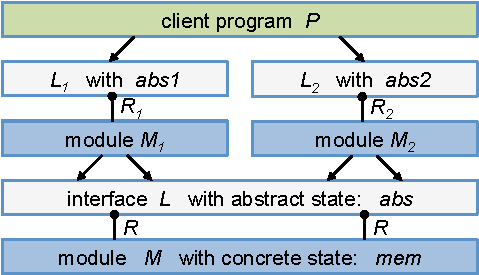
\includegraphics[scale=1]{figs/conflict}
\caption{Client code with conflicting abstract states?}
\label{fig:conflict}
\end{figure}
%%%%%%%%%%%%%%%%%%%%%%%%%%%%%%%%%%%%%%%%%%%%%%%%%%%%%%%%%%%%%%%%

If a module implements an interface with a deep specification, we
would still hide the private memory state from its client, but we also
need to introduce an {\em abstract state} to specify
the full functionality of each primitive in the interface. 

For example, Figure~\ref{fig:queue} shows the implementation of a
concrete thread queue module (in C) and its interface with a deep
specification (in Coq). The local state of the C implementation
consists of 64 thread queues (%
% e.g., a ready queue and many sleep queues, denoted as 
\textsf{tdqp}) and 64 thread control blocks
(\textsf{tcbp}).  Each thread control block consists of the thread state,
and a pair of pointers (\textsf{prev} and \textsf{next}) indicating which
linked-list queue it belongs to. The \textsf{dequeue} function 
takes a pointer to a queue; it returns the head block if the queue
is not empty, or null if the queue is empty.

In the Coq specification (Figure~\ref{fig:queue} right; we omitted some
invariants to make it more readable)\ronghui{Re-draw the figure}, we introduce an abstract state
of type \textsf{abs} where we represent each C array as a Coq finite map
(\textsf{ZMap.t}), and each pointer as an integer index (\textsf{Z}) to the
\textsf{tdq} or \textsf{tcb} array. The \textsf{dequeue} primitive 
$\hat{\sigma}_\textsf{dequeue}$ is
a mathematical function of type $\textsf{abs} \rightarrow \textsf{Z}
\rightarrow \textsf{option (abs}\times \textsf{Z)}$; when the function returns
\textsf{None}, it means that the abstract primitive faults.  This
\textsf{dequeue} specification is intentionally made very similar to the C
function, so we can easily show that the C module indeed {\em
  implements} the specification. 

We define that a module implements a specification if there is a
{\em forward simulation}~\cite{Lynch95} from the module implementation to its
specification. In the context of determinate and receptive 
languages~\cite{sevcik13,Leroy-backend},
if the specification is also deterministic, it is sufficient to find
a forward simulation from the specification to its
implementation (this is often easier to prove in practice). 
In the rest of this thesis, following CompCert, we often call the
forward simulation from the implementation to its specification
as {\em upward (forward) simulation} and the one from the specification
to its implementation as {\em downward (forward) simulation}.


%%%%%%%%%%%%%%%%%%%%%%%%%%%%%%%%%%%%%%%%%%%%%%%%%%%%%%%%%%%%%%%%
\begin{figure}[t]\scriptsize
$$
\begin{array}{l|l}
\hspace*{-2ex} 
\begin{array}[t]{l}
\verb+Definition tcb := td_state.+\\
\verb++\\
\verb+Definition tdq := List Z.+\\
\verb++\\
\verb+Record abs':={tcbp:ZMap.t tcb;+\\
\verb+              tdqp:ZMap.t tdq}+\\
\end{array}
&
\begin{array}[t]{l}
\verb+Function + \hat{\sigma}_\textsf{dequeue}' \verb+ a i :=+\\ 
\verb+match (a.tdqp i) with+\\
\verb+| h :: q' =>+\\
\verb+  Some(set_tdq a i q', h)+\\
\verb+| nil => None+\\
\verb+end ......+\\
\end{array}
\end{array}
$$ 
\caption{A more abstract queue (in Coq)}
\label{fig:queue2}
\end{figure}
%%%%%%%%%%%%%%%%%%%%%%%%%%%%%%%%%%%%%%%%%%%%%%%%%%%%%%%%%%%%%%%%

Figure~\ref{fig:queue2} shows a more abstract specification of the same
queue implementation where the new abstract state \textsf{abs'} omits
the \textsf{prev} and \textsf{next} links in \textsf{tcb} and treats each
queue simply as a Coq list. The \textsf{dequeue} specification 
$\hat{\sigma}_\textsf{dequeue}'$ is now
even simpler, which makes it easier to reason about its client,
but it is now harder to prove that the C module
implements this more abstract specification.  This explains why we
often introduce less abstract specifications (\eg,
the one in Figure~\ref{fig:queue}) as intermediate steps, so a
complex abstraction can be decomposed into several more tractable
abstraction steps.

Deep specification brings out an interesting {\bf new challenge}
shown in Figure~\ref{fig:conflict}: {\em what if a program $P$ attempts to
call primitives defined in two different interfaces $L_1$ and $L_2$,
which may export two conflicting views (i.e., abstract states
\textsf{abs1} and \textsf{abs2}) of the same abstract state \textsf{abs}
(thus also the same concrete memory state \textsf{mem})?}
\ronghui{Concurrency}

Here we assume that modules $M, M_1, M_2$ implement interfaces $L,
L_1, L_2$ via some simulation relations $R, R_1, R_2$ (lines marked
with a dot on one end) respectively. Clearly, calling primitives in
$L_2$ may violate the invariants imposed in $L_1$, and vice versa,
so $L_1$ and $L_2$ are breaking each other's abstraction when we run
$P$. In fact, even without $M_2$ and $L_2$, if we allow $P$ to
directly call primitives in $L$, similar violation of $L_1$ invariants
can also occur.

This means that we must prohibit client programs such as $P$ above,
and each deep specification must state the clear assumptions about its
valid client contexts. Each interface should come with a single
abstract state (\textsf{abs}) used by its primitives; and its client can
only access the same \textsf{abs} throughout its execution. 

This is what {\em abstraction layers} are designed for and why they
are more compositional (with respect to deep specification)
than regular modules! Layers are introduced to limit 
interaction among different modules: only modules with identical
state views (i.e., $R_1, R_2$ and \textsf{abs1},
\textsf{abs2} must be identical) can be composed horizontally.
 
A layer interface seems to be defining a new ``abstract machine''
because it only supports client programs with a particular view of the
memory state. The correctness of a certified layer implementation
allows us to transfer formal reasoning (of client programs) on one
abstract machine (the overlay) to another (the underlay).  

Programming with certified abstraction layers enables a disciplined way of
composing a large number of components in a complex system. Without
using layers, we may have to consider arbitrary module interaction or
dependencies: an invariant held in one function can be easily broken
when it calls a function defined in another module. A layered approach
aims to sort and isolate all components based on a carefully designed
set of abstraction levels so we can reason about one small abstraction
step at a time and eliminate most unwanted interaction and dependencies.



\section{Building Layers for Sequential Kernels}

\begin{figure}[tb] \centering
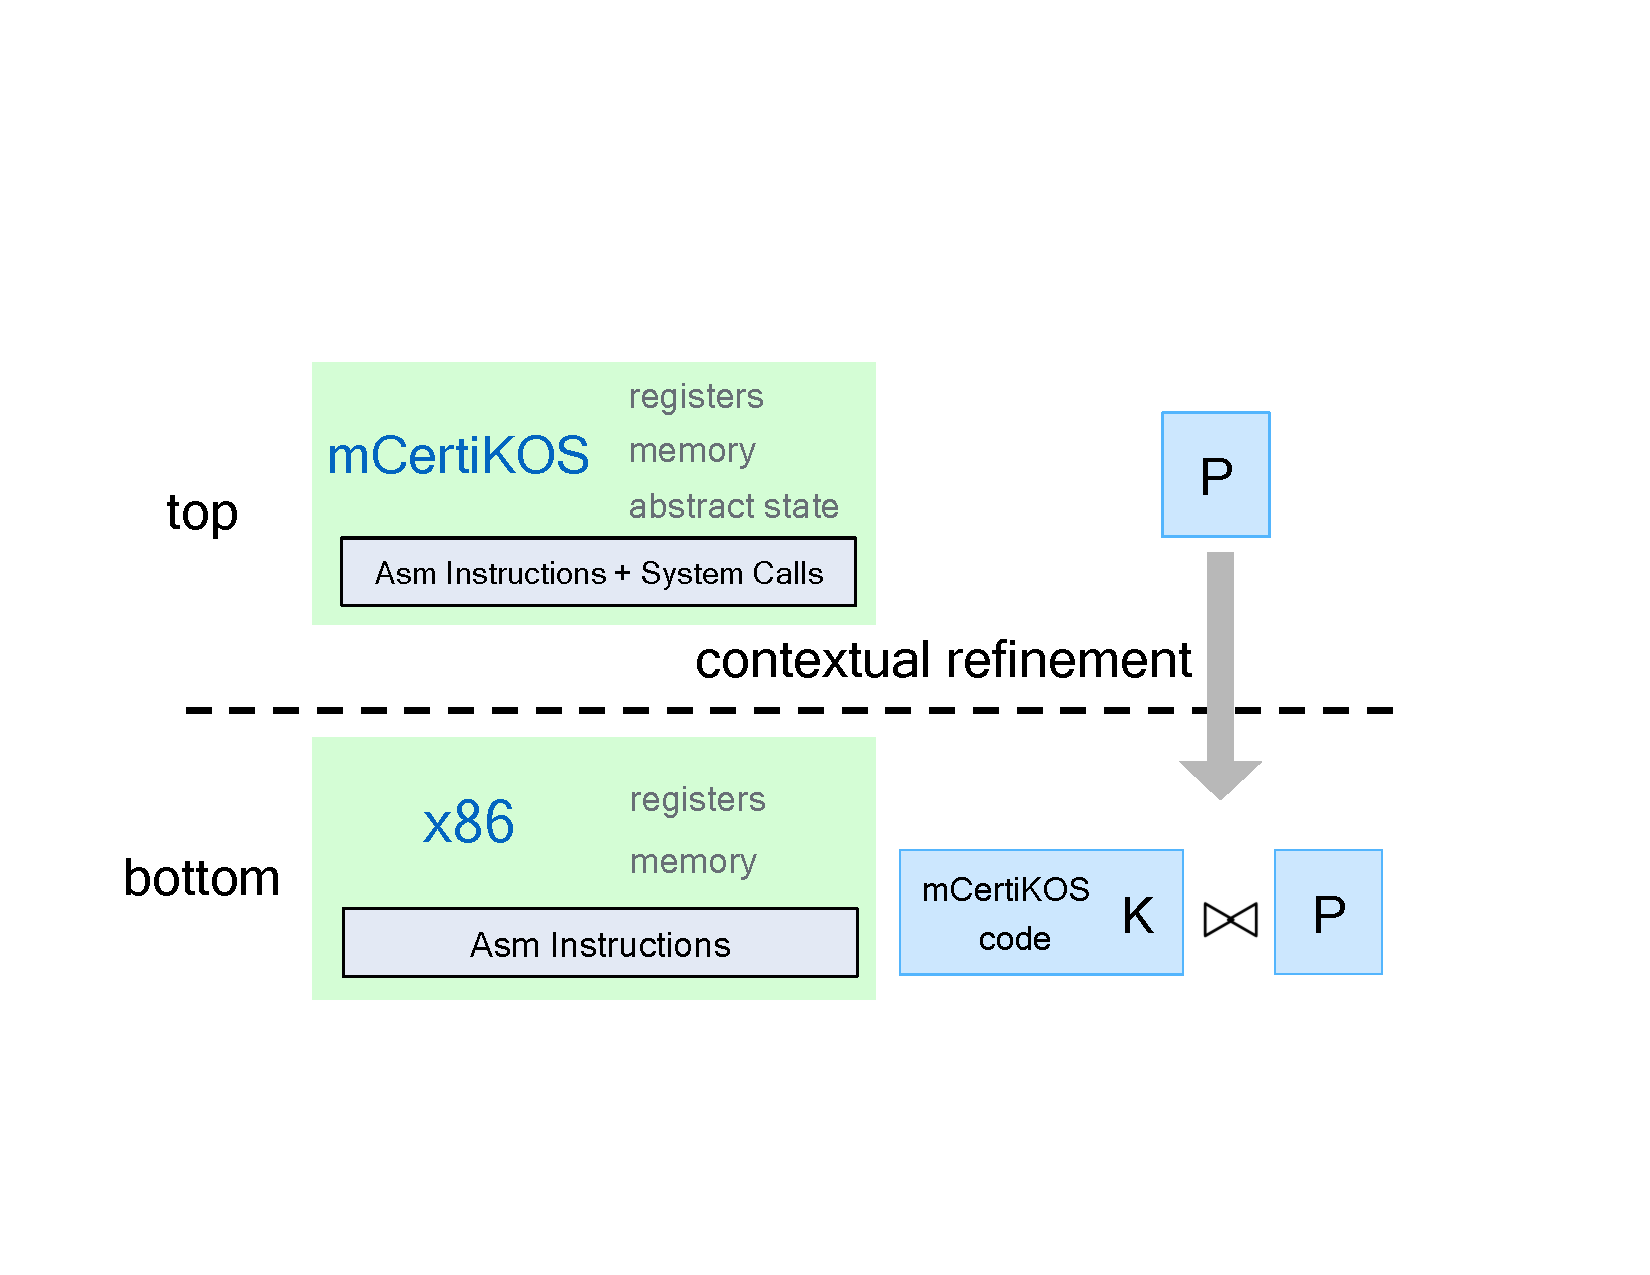
\includegraphics[scale=.5]{figs/mainthm}
\caption{Certified OS kernels: what to prove?}
%\rule[0in]{\columnwidth}{.15mm}
\label{fig:mainthm}
\end{figure}
Under \CTOS, building a new certified kernel (or experimenting with a new
design) is just a matter of composing a collection of certified
layers, developed in a variant of C (called ClightX) or assembly.
\CTOS{} provides  a powerful Coq library
for supporting {\em horizontal} and {\em vertical} composition of
certified layers, as well as a certified compiler (called
CompCertX) that can compile certified ClightX layers into certified
assembly layers. \CTOS\ can thus enjoy the full programming power of
an ANSI C variant and also the assembly language to certify any
efficient routines required by low-level kernel programming.  The
layer mechanism allows us to certify most kernel components at higher
abstraction levels, even though they all eventually get mapped (or
compiled) down to an assembly machine
 that models important hardware details (\eg, virtual memory support).


In Figure~\ref{fig:mainthm}\ronghui{$\oplus$}, we use x86 to denote an assembly machine
and {$\sem{\rm{}x86}{\cdot}$} for its whole-machine semantics.
Suppose we load such a machine with the \mCTOS\ kernel $K$ (in
assembly) and user-level assembly code $P$; then proving any
global property of such a complete system amounts to reasoning about
the semantic object {$\sem{\rm{}x86}{K\join P}$}.

Reasoning at such a low level is difficult, so we formalize a new
\mCTOS\ machine that extends the x86 machine with the deep
specification of $K$. We use $\sem{\rm\mCTOS}{\cdot}$ to denote its
whole-machine semantics.  The contextual refinement property about the
\mCTOS\ kernel can be stated as $\forall
P,\;\sem{\rm{}x86}{K\join{}P}\Refrel{}\sem{\rm\mCTOS}{P}$.
\noindent{}Hence any global property proved about
$\sem{\rm\mCTOS}{P}$ can be transferred to
$\sem{\rm{}x86}{K\join{}P}$.


%Contextual refinement is also a highly general and
%compositional property. Recent work~\cite{filipovic10,liang13} on
%concurrent objects~\cite{herlihy90} has shown that contextual
%refinement is precisely equivalent to the linearazibility and
%various liveness properties~\cite{Herlihy08book}. 

\begin{figure}[tb] \centering
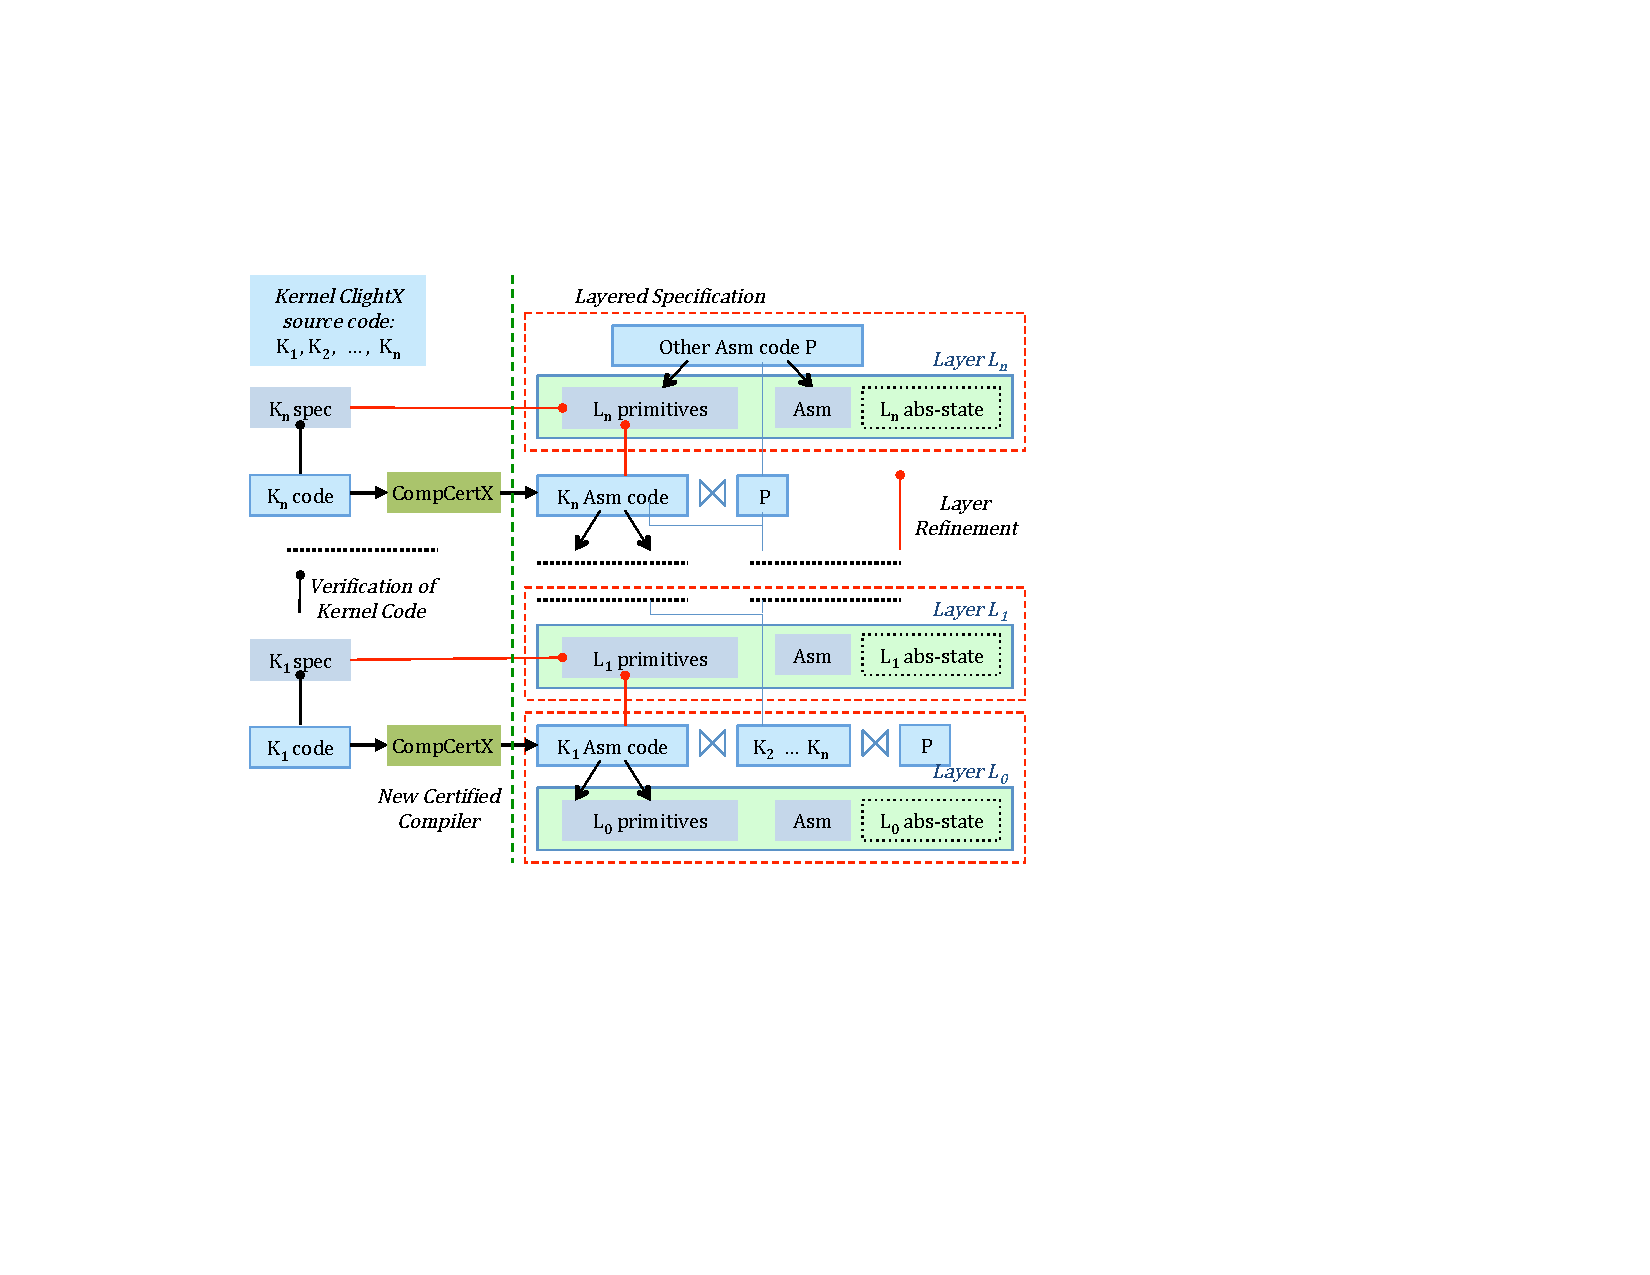
\includegraphics[scale=1]{figs/archA}
\caption{Overview of the \CTOS\ architecture}
%\rule{\columnwidth}{.15mm}
\label{fig:arch}
\end{figure}

In \CTOS, we also use contextual refinement to support fine-grained
layer decomposition and linking.  In Figure~\ref{fig:arch}, to build a
certified kernel $K$, we decompose it into multiple kernel modules
$K_1,...,K_n$, each sitting at its respective underlay ($L_0$, ...,
$L_{n-1}$). Each such module ($K_i$) implements the primitives in its
overlay (\ie, $L_i$) but it can only call the primitives in its
underlay (\ie, $L_{i-1}$).  Using vertical composition~\cite{dscal15}, from
the contextual refinement $\forall
P,\;\sem{i-1}{K_i\join{}P}\Refrel{}\sem{i}{P}$ for each layer (we use
$\sem{j}{\cdot}$ to denote the semantics of the $L_j$ machine), we can
deduce:
$$\forall P, \sem{0}{K\join{}P} =
\sem{0}{K_1\join{}K_2\cdots\join{}K_n\join{}P} \Refrel
\sem{1}{K_2\cdots\join{}K_n\join{}P} \cdots \Refrel
\sem{n-1}{K_n\join{}P} \Refrel \sem{n}{P}$$
If we instantiate $L_0$
and $L_n$ with the x86 and \mCTOS\ layers, we get precisely the
contextual refinement property of the \mCTOS\ kernel. 

We can also
compose intermediate layers in the same way---this makes it much
easier to modify existing (or add new) certified kernel modules.
For example, once the abstract layer interface
for thread queue (\cf{}Figure~\ref{fig:queue2}) is introduced,
there is no need to see (or reason about) 
the concrete queue implementations
and the intermediate interfaces (\cf{}Figure~\ref{fig:queue}). 
Thus, all the code relied on the thread queue module can be verified
at a higher abstraction level using these abstract queue primitives,
which are still {\em realizable} by an efficient assembly implementation
(\ie, Figure~\ref{fig:queue} left).


\ignore{
\begin{figure}[htb]\scriptsize
$$
\begin{array}{l|l}
\begin{array}{l}
\verb+/* memory types */+
\\
\verb+#define MEM_RAM      1+
\\ 
\verb+#define MEM_RESERVED 2+
\\
\verb+#define MEM_ACPI     3+
\\
\verb+#define MEM_NVS      4+ 
\\ 
\verb#struct pmmap {#
\\
\verb#  uintptr_t start;#
\\
\verb#  uintptr_t end;#
\\
\verb#  uint32_t  type;#
\\
\verb#};#                           
\\
\verb#struct pmmap mm[128];#
\end{array}
&
\begin{array}{l}
\verb#Inductive MEMPerm:=#
\\
\verb#| MEM_RESERVED#
\\
\verb#| MEM_USABLE.#
\\
\\
\verb#Inductive pmmap:=#
\\
\verb#| MEMV (start end : Z)#
\\
\verb#       (type : MEMPerm)#
\\
\verb#| MEMUndef.#
\\  
\\
\verb#Definition MM :=#
\\
\verb#       ZMap.t pmmap.#
\end{array}
\\\vspace*{-14pt}
\end{array}
$$ 
\caption{Concrete memory vs. abstract state}
\label{fig:abs-pmmap}
\vspace*{-10pt}
\end{figure}


For example, in $K_1$, we might use an array (in $L_0$ memory) to
implement a physical memory map \verb+mm+ (see Fig.~\ref{fig:abs-pmmap} left,
in C syntax); 
this map describes the physical memory
layout including the size and ``type'' of every memory piece. 
For any code above $L_0$, there is no need to see (or reason
about) such concrete details. Instead, we encapsulate $K_1$
by hiding the array (in $L_0$) and replacing it with a Coq finite map
\verb+MM+ (see Fig.~\ref{fig:abs-pmmap} right) as part of 
the new abstract state in $L_1$. Note, we only need to 
know which memory piece is usable or reserved (\verb+MEMPerm+), 
and we need to add the case \verb+MEMUndef+ to represent the content
of \verb+mm+ before it is initialized. Here \verb+Z+ and \verb+ZMap.t+ 
are Coq's integer and finite map types. The new $L_1$ primitives
can then be specified using the Coq finite map
so $L_1$ code can be verified
at a higher abstraction level, but these primitives
are still {\em realizable} by an efficient assembly implementation
(i.e., $K_1$).}

This last point is important since it means that abstraction
layers in \CTOS\ are introduced strictly to support compositional 
specification and verification. Regardless how many layers we add 
and how we specify the layer primitives, the kernel always has the same 
efficient assembly implementation.

\section{Building Layers for Concurrent Kernels}
\label{sec:overview:concurrent}
To build certified concurrent OS kernels,
we introduce a notion of \emph{certified concurrent abstraction
layer}: a special abstraction layer that 
contains a \emph{shared
global log} to record the shared operations
of the whole system.

\paragraph{Concurrent abstraction layers}
Like a general abstraction layer layer, each concurrent layer can also
contain thread-private abstract states (refined from the concrete
thread-local in-memory data) and related abstract primitives. However,
the data shared by multiple threads are not represented as abstract
states. Instead, each method call to a shared atomic object is
recorded as an observable event and is appended to the end of a shared
global log. For each shared object, we define a {\em replay} function
that can reconstruct the current shared state from the current global
log. Thus, all shared objects are represented as a single sequence of
logged events with appropriate replay functions.

With concurrency, the machine semantics for each layer (e.g.,
$\sem{L}{\cdot}$) is no longer deterministic: for each scheduler
strategy ($\strat{hs}$), it may generate a different global
log. To prove the simulation $\sem{L'}{P\oplus{}M} \leq_R \sem{L}{P}$,
for each scheduler strategy $\strat{hs}$, if running $P\oplus{}M$ on
machine $L'$ with $\strat{hs}$ produces a global log $l$, we must find
another scheduler strategy $\stratp{hs}$ such that running $P$ on
machine $L$ under $\stratp{hs}$ would generate a global log $l'$ that
is related to $l$ via the simulation relation $R$. We will actually
construct a {\em function} that will map $l$ and $\strat{hs}$ into
$l'$ and $\stratp{hs}$. Of course, the simulation relation $R$ over
thread-private states might still be a relation~\cite{dscal15}.

\paragraph{An example of concurrent layers}
The example in Figure~\ref{fig:exp:ticket_lock_example} contains a
client program $P$ which has two threads running on two different
CPUs; each thread makes one call to the atomic primitive $\comm{foo}$
provided by the layer interface $L_3$.

Concurrent object module $M_2$ implements the layer interface $L_3$
but it is built on top of $L_2$.  The $\comm{foo}$ method calls two
atomic primitives $f$ and $g$ in a critical section protected by a
ticket lock~\cite{mcs91}.

%%%%%%%%%%%%%%%%%%%%%%%%%%%%%%
\begin{figure}
\lstinputlisting [language = C, multicols=2] {source_code/ticket_lock_example.c}
%\vspace{-5pt}
\caption{Building certified concurrent layers over a ticket lock}
\label{fig:exp:ticket_lock_example}
\vspace{-10pt}
\end{figure}
%%%%%%%%%%%%%%%%%%%%%%%%%%%%%%

The ticket-lock module $M_1$ is built on top of $L_1$ and it
implements $L_2$. Even though the implementation of a ticket lock
contains two shared integer value fields: $\comm{ticket}$ and
$\comm{now}$ (where $\comm{now} \leq \comm{ticket}$ always holds), the
interface $L_1$ only provides the atomic primitives such as
fetch-and-incrementing the $\comm{ticket}$ value, getting the current
$\comm{now}$ value, holding the lock (if the $\comm{now}$ value is
equal to the $\comm{ticket}$ value), and incrementing the $\comm{now}$
value (to release the lock). The current $\comm{ticket}$ and
$\comm{now}$ values can be reconstructed by replaying the global log
(for the $L_1$ machine).  $L_1$ also provides the atomic $\comm{f}$
and $\comm{g}$ events which are later passed on to $L_2$.

\paragraph{Strategy, environment context, and layer simulation}
Our goal is to show that for each run of $P\oplus{}M_2\oplus{}M_1$
over $L_1$, we can find another run of $P$ over $L_3$ so that the
global logs produced by both runs are related.
To show how we accomplish this, here is
a global log $l_{g1}$ produced from  
a specific run of $P\oplus{}M_2\oplus{}M_1$ over $L_1$.

\vspace*{-1ex}
% \colorbox{Peach}{\textcolor{white}{a}}
\begin{small}
\[
\begin{array}{l}
\ssame \cons (1.\incticket) \cons
\sdiff \cons (2.\incticket) \cons
\ssame \cons (2.\getnow) \cons
\sdiff \cons (1.\getnow) \cons
\ssame \cons (1.\holdlock) 
\\
\cons 
\sdiff \cons (2.\getnow) \cons
\sdiff \cons (1.\comm{f}) \cons
\sdiff \cons (2.\getnow) \cons
\sdiff \cons (1.\comm{g}) \cons
\ssame \cons (1.\incnow) 
\\
\cons \sdiff \cons (2.\getnow) \cons
\ssame \cons (2.\holdlock) \cons
\ssame \cons (2.\comm{f}) \cons
\ssame \cons (2.\comm{g}) \cons
\ssame \cons (2.\incnow) 
\end{array}
\]
\end{small}%

Throughout this paper, we assume that all programs always
start from CPU 1, and before each CPU executes an atomic primitive,
it always yields to the hardware scheduler ($hs$).
We use $\ssame$ to denote a hardware yield to the same CPU,
and $\sdiff$ for a yield to a different CPU; each such symbol
is actually an abbreviation of two consecutive switch events: switch
from CPU $i$ to $hs$ (\ie, $i\switch{}hs$), and then switch from $hs$
to CPU $j$ (\ie, $hs \switch j$).  For example, starting from CPU 1,
$\sdiff$ is an abbreviation of $(1\switch{}hs) \cons (hs\switch 2)$.

We define $\comm{target}(l)$ as the switching destination of the last event in
the log $l$, which can be either 1, 2, or $hs$. The above run,
which produced the global log $l_{g1}$, can be viewed as combining
the following {\em strategies} defined for each CPU and $hs$:

\vspace*{-1ex}
\begin{small}
\[
\strat{j} (l)=
\begin{cases}
  j.e & \text{if } (\comm{target}(l) = j) ~~\wedge \\
      & ~~~~~(l\cons (j.e)) |_{j,hs} \text{ is a prefix of } (l_{g1} |_{j,hs}) \\
\comm{undefined } & \text{otherwise}
\end{cases}
\]
\end{small}%

\noindent{}Here, $l |_{j,hs}$ only keeps those events in $l$ that are
related to participants $j$ and $hs$.  For the hardware scheduler's
strategy $\strat{hs}$, this filtering essentially means that
regardless how the CPUs (or threads) are going to play in the interim,
$hs$'s moves will always follow $l_{g1}$.  Because $\strat{hs}$
defines how switching between different CPUs is done, when we define
each CPU's strategy, we filter out other CPUs' events but still keep
those events related to $hs$.

At each step, depending on the destination ($j$) of the current log
($l$), we can query the corresponding strategy $\strat{j}(l)$ to get the
next move for $j$.  For example, if the destination is $hs$, that is,
the log ends with $(\any\switch hs)$, then it is the
hardware scheduler's turn to generate a switch event $(hs\switch \any)$.

These strategies also form a nice decomposition of the global log
$l_{g1}$. To reason about CPU 1 alone, we only need to construct
its environment context $\oracle_1 := \strat{hs} \bigcup \strat{2}$.

The layer interface $L_2$ introduces the $\acq$ and $\rel$ primitives
which trigger events $\acq$ and $\rel$ respectively. Running
$P\oplus{}M_2$ over $L_2$ could produce the following shared log $l_{g2}$:

\vspace*{-1ex}
\begin{small}
\[
\begin{array}{l}
\ssame \cons (1.\acq) \cons
\ssame \cons (1.\comm{f}) \cons
\ssame \cons (1.\comm{g}) \cons
\ssame \cons (1.\rel) 
\\
\cons \sdiff \cons (2.\acq) \cons
\ssame \cons (2.\comm{f}) \cons
\ssame \cons (2.\comm{g}) \cons
\ssame \cons (2.\rel) 
\end{array}
\]
\vspace{-5pt}
\end{small}%

The layer interface $L_3$ introduces the atomic $\comm{foo}$
primitive. Running $P$ over $L_3$ could produce the following shared log
$l_{g3}$:
\vspace*{-1ex}
\begin{small}
\[
\ssame \cons (1.\comm{foo})
\cons \sdiff \cons (2.\comm{foo})
\]
\vspace{-7pt}
\end{small}%

To build a simulation, we want to define a function mapping one
layer's log and environment context into those of another layer.  For
example, the function $f_l$, mapping a log over $L_1$ into one over
$L_2$, can be defined as follows: (1) it maps the $\holdlock$ and
$\incnow$ events in $L_1$ to $\acq$ and $\rel$ events in $L_2$; (2) it
drops the $\incticket$ and $\getnow$ events; 
and (3) it merges all the adjacent switch symbols (\eg,
$\ssame \cons \sdiff$ is merged into $\sdiff$).
The following shows that $l_{g2} = f_l (l_{g1})$ is true:

\vspace*{-1ex}
\begin{small}
\[
\begin{array}{l}
\hspace*{-1em}\mysout
{\ssame \cons (1.\incticket) \cons
\sdiff \cons (2.\incticket) \cons
\ssame \cons (2.\getnow) \cons
\sdiff \cons (1.\getnow) \cons
}
\ssame \cons (1.\cancel{\holdlock}/\acq) 
\\
\hspace*{-1em}\mysout
{\cons 
\sdiff \cons (2.\getnow) \cons
\sdiff 
} 
\ssame \cons (1.\comm{f}) \cons
\mysout
{\sdiff \cons (2.\getnow) \cons
\sdiff
}
\ssame \cons (1.\comm{g}) \cons
\ssame \cons (1.\cancel{\incnow}/\rel) 
\\
\hspace*{-1em}\cons \sdiff 
\mysout
{\cons (2.\getnow) \cons
\ssame 
}
\cons (2.\cancel{\holdlock}/\acq) \cons
\ssame \cons (2.\comm{f}) \cons
\ssame \cons (2.\comm{g}) \cons
\ssame \cons (2.\cancel{\incnow}/\rel) 
\end{array}
\]
\end{small}

From $f_l$, we can construct a function $f_{\strat{}}$
that maps each strategy $\strat{j}$ for $L_1$ into one for $L_2$:

\vspace*{-1ex}
\begin{small}
\[ 
f_{\strat{}}(\strat{j}) (l'')=
\begin{cases}
j.e' & \text{if } 
\exists l', f_l(l') = l'' \wedge \strat{j}(l') = j.e\\
&\qquad\ \wedge f_l(l'\cons(j.e)) = l'' \cons (j.e') \\
\comm{undefined } & \text{otherwise}
\end{cases}
\]
\end{small}

Here, since many $L_1$ events are dropped in $L_2$,
the $L_2$ strategy $f_{\strat{}}(\strat{j})$ for $j$
has to keep querying $\strat{j}$ until
it also returns an event from $j$ at $L_2$.  For example, let $l'$ be
$\ssame \cons (1.\incticket) \cons \sdiff \cons (2.\incticket) \cons
\ssame \cons (2.\getnow) \cons \sdiff \cons (1.\getnow) \cons \ssame$,
since $\strat{1} (l') = 1.\holdlock$ and $f_l(l') = \ssame$, we have
$f_{\strat{}}(\strat{1}) (\ssame) =1.\holdlock$.

Finally, from $f_{\strat{}}$ we can construct the function
$f_{\oracle}$ which will map each environment context $\oracle$ for
$L_1$ into one for $L_2$.

\paragraph{Layer verification and composition}
Reasoning about a concrete strategy is simple, but when we verify
a concurrent module, we cannot assume such a specific environment context.
Instead, to verify
a layer running on CPU~$i$, we have to show that its implementation
meets its specification for all possible environment contexts
$\oracle_i$ that satisfy its ``rely'' invariants.

For example, to show that $\ltyp{L_1[1]}{R}{M_1}{L_2[1]}$, we must
show that the implementation of $\acq$ meets its specification.
This requires us to prove the starvation-freedom of the ticket
lock algorithm. To do so, we can impose the following rely conditions
over $\oracle_1$:
%%%%%%
\begin{itemize} \itemsep 0pt
\item ($\comm{INV}_{hs}$):  $\strat{hs}$ is \emph{fair}, that is,
  for any CPU $i$, the gap between two $(hs \switch i)$ events
  in the log is less than some constant $m$.
%%%%%%%
\item ($\comm{INV}_{2}$):  $\strat{2}$ will eventually release the
  lock it held, that is, the number of events generated by CPU~2
  between $(2.\holdlock)$ and $(2.\incnow)$   is less
  than some constant $n$ .
\end{itemize}
%%%%
Therefore, when CPU~1 acquires the lock, the loop iteration (\cf
line 17 in Fig~\ref{fig:exp:ticket_lock_example}) is bound by
$n \times m$, because CPU~2 can generate at most $n$ events before
releasing the lock and $\strat{hs}$ is fair to CPU~2.

Interestingly, we do not need
to prove that CPU~1 \emph{guarantees} to release the lock within $n$
steps in machine $L_2[1]$
when we prove $\ltyp{L_1[1]}{R}{M_1}{L_2[1]}$.  We can restore
this guarantee proof when we prove $\ltyp{L_2[1]}{R}{M_2}{L_3[1]}$
since clearly, each call to $\acq$ in $M_2$ is followed by a call to
$\rel$ within three steps.

Two certified layers are allowed to compose only if each one's guarantee
implies the other's rely. We cannot parallel-compose
$\ltyp{L_1[1]}{R}{M_1}{L_2[1]}$ and $\ltyp{L_1[2]}{R}{M_1}{L_2[2]}$;
but we can first get $\ltyp{L_1[1]}{R}{M_1\oplus{}M_2}{L_3[1]}$ and
$\ltyp{L_1[2]}{R}{M_1\oplus{}M_2}{L_3[2]}$, and then compose these to
get $\ltyp{L_1[T]}{R}{M_1\oplus{}M_2}{L_3[T]}$.







\ignore{
\paragraph*{What have we proved?}
Using \CTOS, we have successfully built multiple certified OS
kernels. For each such kernel, we have always constructed its deep
specification and proved its contextual functional correctness
property, so all global properties proved at the specification level can
be transferred down to the lowest assembly machine.

From the functional correctness property, we immediately derive that
all system calls and traps will always run {\em safely} and also
terminate; and there will be no code injection attacks, no buffer
overflows, no null pointer access, no integer overflow, etc. We also
proved that there is no stack overflow or memory exhaustion in the
kernel using recent techniques developed by Carbonneaux~{\em et
  al}~\cite{veristack,ccrb15}.  As we will discuss in
Sec.~\ref{security}, we also proved an isolation property between the
virtual address spaces of user-level processes.  All of these
properties were proved using the abstract specification provided at
the top layer, and then transferred to the lowest assembly machine via
contextual refinement.}
\chapter{Sequential CertiKOS Framework}
\label{chap:seq}
In this Chapter, we will provide the formal details
of our sequential \CTOS{} framework.
Section~\ref{sec:seq:layer} introduces
a layer calculus to compose
sequential layers vertically and
horizontally, starting from \emph{layer semantics unit}
(which is language dependent).
This layer calculus is general enough,
such that it is not bounded to any specific language,
and the components of layer interfaces
and types of primitives are treated as parameters. 
In Section~\ref{sec:seq:sound},
we show the proof structure for the soundness of layer calculus.
Section~\ref{sec:seq:clight}
and Section~\ref{sec:seq:lasm}
show how to construct layer semantics unit
and apply layer calculus
in ClightX (\ie, a C-like language) and LAsm (\ie, an assembly language), respectively.
In Section~\ref{sec:seq:comp},
we introduce CompCertX (\ie, a verified C compiler)
to compile ClightX layers down to assembly-level,
and show how to link the result layers with
LAsm layers.

\section{A Calculus of Sequential Abstraction Layers}
\label{sec:seq:layer}

\paragraph{Motivation}

A user of an abstraction layer $\layer{L_1}{M}{L_2}$ wants to know
that its implementation $M$ (on top of the underlay interface $L_1$)
can be used to run any program $P$ written against the overlay
interface $L_2$.
If we consider $L_1, L_2$ as abstract machines
and $M$ as a program transformation (which transforms
a program $P$ into $M(P)$), 
then for some notion of refinement $\sqsubseteq$,
this property can be stated as
$\forall P \,.\, M(P) @ L_1 \sqsubseteq P @ L_2$,
meaning that the behavior of $M(P)$ executing
on top of the underlay specification $L_1$
refines that of the program $P$
executing on top of the overlay specification $L_2$.

This view of abstraction layers captures a wide variety of situations.
Furthermore, two layers $\layer{L_1}{M}{L_2}$ and
$\layer{L_2}{N}{L_3}$ can be composed as $\layer{L_1}{M \circ
  N}{L_3}$, and the correctness of the layer implementation $M \circ
N$ follows from that of $M$ and $N$.  
%This gives us a way to decompose
%layer implementations into a succession of smaller and
%easier-to-verify components.

However, 
% this paradigm is ill-suited for implementation purposes.
% An unrestricted program transformation is often too
% general to describe what is actually going on: 
the layer interfaces
are often not arbitrary abstract machines, but simply instances of a base
language, specialized to provide layer-specific primitives and
abstract state.  The implementation is not an arbitrary
transformation, but instead consists of some library code to be linked
with the client program.  In order to prove this transformation correct,
we will verify the implementation of each primitive
separately, and then use these proofs in conjunction with a
general template for the instrumented language.

Abstract machines and program transformations are too general to
capture this redundant structure.  The sequential layer calculus
presented in this section provides fine-grained notions of layer
interfaces and implementations.  It allows us to describe what varies
from one layer to the next and to assemble such layers 
%from their components 
in a generic way.

\subsection{Prerequisites}

To keep the formalism general and simple,
we initially take the syntax and behavior of the programs
under consideration to be abstract parameters.
Specifically,
in the remainder of this section we will assume that
the following are given:
\begin{itemize}
\item a set of identifiers $i \in \integer$
    which will be used to name variables, functions, and primitives
    (\eg, \textsf{deQ} and \textsf{tcbp} in Figure~\ref{fig:queue});
\item sets of function definitions $\kappa \in \mathbb{K}$ and
    variable definitions $\nu \in \mathbb{T}$,
    as specified by the language
    (\eg, $\kappa_\textsf{deQ}$ and $\nu_\textsf{tcbp}$ in Figure~\ref{fig:queue});
% XXX: identifiers?
\item a set of behaviors $\sigma \in \Sigma$
    for the individual primitives of layers
    and the individual functions of programs
    (\eg, the step relation $\sigma_\textsf{deQ}$ 
    	derived from the Coq function 
    	$\spec_\textsf{deQ}$ in Figure~\ref{fig:queue}).
\end{itemize}
For example, in the model given in Section~\ref{sec:seq:clight},
we will use step relations as the behaviors.
Function definitions will include the functions' formal parameters and bodies
(but not their names),
whereas definitions of variables
will specify their types and initialization data.
% XXX: but for now completely abstract

We also need to define how the behaviors
refine one another.
This is particularly important because
our layer interfaces bundle primitive specifications,
and because a relation between layer interfaces is defined pointwise
over these primitives. Ultimately, we wish to use these
fine-grained layers and refinements to build complete abstract
machines and whole-machine simulations. 
%FIXME: improve:
%Yet, ultimately we wish to use these
%fine-grained layers and refinements
%to build complete abstract machines and whole-machine simulations.
This can only be done
if the refinements of individual primitives are consistent;
for example, if they are given in terms of the same simulation relation.

Hence, we index behavior refinement by
the elements of a partial monoid $(\mathbb{R}, \circ, \id)$.
We will refer to the elements $R \in \mathbb{R}$ of this monoid
as \emph{simulation relations}.
However, note that at this stage,
the elements of $\mathbb{R}$ are entirely abstract,
and we require only that the composition operator $\circ$
and identity element $\id$ satisfy the monoid laws
$R_1 \circ (R_2 \circ R_3) = (R_1 \circ R_2) \circ R_3$ and
$R \circ \id = \id \circ R = R$.

Finally,
we need to interpret these abstract simulation relations
as refinement relations between behaviors.
That is,
for each $R \in \mathbb{R}$, we require
a relation $\lpath{R}$ on $\Sigma$.
For instance,
if the behaviors $\sigma_1, \sigma_2 \in \Sigma$
are taken to be step relations over some sets of states,
$\sigma_1 \le_R \sigma_2$ may be interpreted
as the following simulation diagram:
\[ 
    \xymatrix{
        s_1 \ar[rr]^{\sigma_1} \ar@{-}[d]_R & & s'_1 \ar@{.}[d]^R \\
        s_2 \ar@{.>}[rr]_{\sigma_2} & & s'_2
    }
\]
That is, whenever two states $s_1, s_2$
are related by $R$ in some sense,
and $\sigma_1$ takes $s_1$ to $s_1'$ in one step, then
there exists $s_2'$ such that 
$\sigma_2$ takes $s_2$ to $s_2'$ in zero or more steps,
and $s_2'$ and $s_1'$ are also related by $R$.
The relations $\le_-$ should respect the monoid structure of $\mathbb{R}$,
so that for any $\sigma \in \Sigma$ we have $\sigma \lpath{\id} \sigma$,
and so that whenever $R, S \in \mathbb{R}$
and $\sigma_1, \sigma_2, \sigma_3 \in \Sigma$
such that $\sigma_1 \lpath{R} \sigma_2$ and $\sigma_2 \lpath{S} \sigma_3$,
it should be the case that $\sigma_1 \lpath{S \circ R} \sigma_3$.
% XXX: Possibly summarize laws in a figure instead?

\subsection{Sequential layer interfaces and modules}
\begin{figure}[t]
    \begin{align*}
        \lfloor L \rfloor \in \mathbb{L} &=
            \mathbb{I} \rightharpoonup (\Sigma + \mathrm{T}) &
        \lfloor M \rfloor \in \mathbb{M} &=
            \mathbb{I} \rightharpoonup (\mathrm{K} + \mathrm{T}) \\
        %
        \lfloor \varnothing \rfloor &=
            \bot &
        \lfloor \varnothing \rfloor &=
            \bot \\
        %
        \lfloor i \mapsto \sigma \rfloor &=
            i \mapsto \iota_1(\sigma) &
        \lfloor i \mapsto \kappa \rfloor &=
            i \mapsto \iota_1(\kappa) \\
        %
        \lfloor i \mapsto \nu \rfloor &=
            i \mapsto \iota_2(\nu) &
        \lfloor i \mapsto \nu \rfloor &=
            i \mapsto \iota_2(\nu) \\
        %
        \lfloor L_1 \oplus L_2 \rfloor &=
            \lfloor L_1 \rfloor \cup \lfloor L_2 \rfloor &
        \lfloor M_1 \oplus M_2 \rfloor &=
            \lfloor M_1 \rfloor \cup \lfloor M_2 \rfloor \\
        \lfloor L_1 \lpath{R} L_2 \rfloor &\!\Leftrightarrow
            \lfloor L_1 \rfloor \lpath{R} \lfloor L_2 \rfloor &
        \lfloor M_1 \subseteq M_2 \rfloor &\!\Leftrightarrow
            \lfloor M_1 \rfloor \sqsubseteq \lfloor M_2 \rfloor
    \end{align*}
    \begin{center}
    Where $\lfloor L_1 \rfloor \lpath{R} \lfloor L_2 \rfloor$ means that for all $i \in \mathbb{I}$:
    \begin{align*}
        \forall \sigma_1 \, . \quad
            \lfloor L_1 \rfloor (i) &= \iota_1(\sigma_1) &\Rightarrow\quad
        \exists \sigma_2 \, . \,
            \lfloor L_2 \rfloor (i) &= \iota_1(\sigma_2) \wedge
            \sigma_1 \lpath{R} \sigma_2 \\
        \forall \nu \, . \quad
             \lfloor L_1 \rfloor (i) &= \iota_2(\nu) &\Rightarrow\quad
             \lfloor L_2 \rfloor (i) &= \iota_2(\nu),
    \end{align*}
    and both orders hold when the right-hand side is undefined.
    \end{center}
    \caption{Interpretation of layers and modules as finite maps}
    \label{fig:fmap-layers}
\hrulefill
    \afterpage{\FloatBarrier}
\end{figure}

The syntax of the calculus is defined as follows:
\[\begin{array}{rl}
    L &::= \varnothing
            \ |\ i \mapsto \sigma
            \ |\ i \mapsto \nu
            \ |\ L_1 \oplus L_2 \\
    M &::= \varnothing
            \ |\ i \mapsto \kappa
            \ |\ i \mapsto \nu
            \ |\ M_1 \oplus M_2
\end{array}\]
\noindent{}The layer interfaces $L$ and modules $M$
are essentially finite maps;
constructions of the form $i \mapsto \_$
are elementary single-binding objects,
and $\oplus$ computes
the union of two layers or modules.
This is illustrated by the proof-of-concept
interpretation given in 
Figure~\ref{fig:fmap-layers}.
For example, the sequential thread queue module, shown in Figure~\ref{fig:queue},
can be defined as 
$M_\textsf{thread\_queue}:=\textsf{tcbp}\mapsto \nu_\textsf{tcbp} 
\oplus \textsf{tdqp}\mapsto \nu_\textsf{tdqp}
\oplus \textsf{deQ}\mapsto \kappa_\textsf{deQ}$,
while the overlay interface can be defined as 
$L_\textsf{thread\_queue}:= \textsf{deQ}\mapsto \sigma_\textsf{deQ}$ .

\begin{figure} [t]
    \noindent
    \fbox{$M_1 \subseteq M_2$}
    \vspace*{-17pt}
    \begin{align*}
        M &\subseteq M &
            \rulename{MLe-Refl} \\
        \varnothing &\subseteq M &
            \rulename{MLe-Empty} \\
        M \oplus \varnothing &\subseteq M &
            \rulename{MLe-Id-Right} \\
        (M_1 \oplus M_2) \oplus M_3 &\subseteq M_1 \oplus (M_2 \oplus M_3) &
            \rulename{MLe-Assoc} \\
        M_2 \oplus M_1 &\subseteq M_1 \oplus M_2 &
            \rulename{MLe-Comm} \\
        M_1 &\subseteq M_1 \oplus M_2 &
            \rulename{MLe-Ub-Left} \\
        M_1 \subseteq M_2 \wedge M_2 \subseteq M_3
            &\Rightarrow M_1 \subseteq M_3 &
            \rulename{MLe-Trans} \\
        M_1 \subseteq M_1' \wedge M_2 \subseteq M_2'
            &\Rightarrow M_1 \oplus M_2 \subseteq M_1' \oplus M_2'
            &\rulename{MLe-Mon}
    \end{align*}

    \vspace{1em}
    \noindent
    \fbox{$L_1 \lpath{R} L_2$}
    \vspace*{-17pt}
    \begin{align*}
        L &\lpath{\id} L &
            \rulename{LLe-Refl} \\
        \varnothing &\lpath{R} L &
            \rulename{LLe-Empty} \\
        L \oplus \varnothing &\lpath{\id} L &
            \rulename{LLe-Id-Right} \\
        (L_1 \oplus L_2) \oplus L_3 &\lpath{\id} L_1 \oplus (L_2 \oplus L_3) &
            \rulename{LLe-Assoc} \\
        L_2 \oplus L_1 &\lpath{\id} L_1 \oplus L_2 &
            \rulename{LLe-Comm} \\
        L_1 &\lpath{\id} L_1 \oplus L_2 &
            \rulename{LLe-Ub-Left} \\
        L \oplus L &\lpath{\id} L &
            \rulename{LLe-Idempotent} \\
        L_1 \lpath{R} L_2 \wedge L_2 \lpath{S} L_3 &\,\Rightarrow\,
            L_1 \lpath{S \circ R} L_3 &
            \rulename{LLe-Trans} \\
        L_1 \lpath{R} L_1' \wedge L_2 \lpath{R} L_2' &\,\Rightarrow\,
            L_1 \oplus L_2 \lpath{R} L_1' \oplus L_2' \hspace{-2em} &
            \rulename{LLe-Mon} \\
        \sigma_1 \lpath{R} \sigma_2 &\,\Rightarrow\,
            i \mapsto \sigma_1 \lpath{R} i \mapsto \sigma_2 &
            \rulename{LLe-Intro-Prim}
    \end{align*}

    \vspace{1em}
    \noindent
    \fbox{$\ltyp{L_1}{R}{M}{L_2}$}
    \vspace*{-17pt}
    \begin{prooftree}
        \AxiomC{}
	\RightLabel{\rulename{Empty}}
 	\UnaryInfC{$\ltyp{L}{\id}{\varnothing}{L}$}
    \end{prooftree}
    \begin{prooftree}
        \AxiomC{}
        \RightLabel{\rulename{Var}}
        \UnaryInfC{$\ltyp{L}{\id}{i \mapsto \nu}{i \mapsto \nu}$}
    \end{prooftree}
    \begin{prooftree}
        \AxiomC{$\ltyp{L_1}{R}{M}{L_2}$}
        \AxiomC{$\ltyp{L_2}{S}{N}{L_3}$}
        \RightLabel{\rulename{Vcomp}}
        \BinaryInfC{$\ltyp{L_1}{R \circ S}{M \oplus N}{L_3}$}
    \end{prooftree}
    \begin{prooftree}
        \AxiomC{$\ltyp{L}{R}{M}{L_1}$}
        \AxiomC{$\ltyp{L}{R}{N}{L_2}$}
        \RightLabel{\rulename{Hcomp}}
        \BinaryInfC{$\ltyp{L}{R}{M \oplus N}{L_1 \oplus L_2}$}
    \end{prooftree}
    \begin{prooftree}
        \AxiomC{$L_1 \lpath{R} L_1'$}
        \AxiomC{$\ltyp{L_1}{S}{M}{L_2}$}
        \AxiomC{$L_2' \lpath{T} L_2$}
        \RightLabel{\rulename{Conseq}}
        \TrinaryInfC{$\ltyp{L_1'}{R \circ S \circ T}{M}{L_2'}$}
    \end{prooftree}
    \caption{The fine-grained layer calculus}
    \label{fig:llang}
\hrulefill
    \afterpage{\FloatBarrier}
\end{figure}

The rules are presented in Figure~\ref{fig:llang}.
The inclusion preorder defined on modules
corresponds to the intuition that when $M \subseteq N$,
any definition present in $M$ must be present in $N$ as well.
The composition operator $\oplus$
behaves like a join operator.
However, while $M \oplus N$ is an upper bound of $M$ and $N$,
we do not require it to be the \emph{least} upper bound.
The order on layer interfaces
extends the underlying simulation preorder $\lpath{R}$ on behaviors.
Compared to $\subseteq$, it should satisfy
the additional property \rulename{LLe-Idempotent}.

The judgment $\ltyp{L_1}{R}{M}{L_2}$ is akin to a typing judgment for
modules. It asserts that, using the simulation relation $R$, the
module $M$---running on top of $L_1$---faithfully implements $L_2$.
Because modules consist of code ultimately intended to be linked
with a client program, the empty module $\varnothing$ acts as a
unit and can implement any layer interface $L$ 
(\rulename{Empty}).  Moreover, appending first $N$ then $M$ to a
client program is akin to appending $M \oplus N$ in one step
(\rulename{Vcomp}).  These rules correspond to the identity and
composition properties already present in the framework of abstract
machines and program transformations.  However, the fine-grained
calculus also provides a way to split refinements (\rulename{Hcomp}):
when two different layer interfaces are implemented \emph{in a
  compatible way} by two different modules on top of a common underlay
interface, then the union of the two modules implements the union of
the two interfaces.

This allows us to break down the problem of verifying a layer
implementation in smaller pieces, but ultimately, we need to handle
individual functions and primitives.  The consequence rule
(\rulename{Conseq}) can be used to tie our notion of behavior
refinement into the calculus.  However, to make the introduction of
certified code possible, we need a semantics of the underlying
language.

\subsection{Language semantics}
\label{ssec:layer-langsem}

\begin{figure}[t]
\begin{align*}%
\llbracket - \rrbracket &\ \,:\ \,\mathbb{M} \rightarrow (\mathbb{L} \rightarrow \mathbb{L}) \\
        i \mapsto \nu &\lpath{\id}
            \llbracket i \mapsto \nu \rrbracket L &
            \rulename{Sem-Var} \\
        \llbracket M \rrbracket (L \oplus \llbracket N \rrbracket L)
            &\lpath{\id}
            \llbracket M \oplus N \rrbracket L &
            \rulename{Sem-Comp} \\
        M_1 \subseteq M_2 \wedge L_1 \lpath{R} L_2 &\,\Rightarrow\,
            \llbracket M_1 \rrbracket L_1 \lpath{R}
            \llbracket M_2 \rrbracket L_2 &
            \rulename{Sem-Mon}%
\end{align*}
\caption{Semantics of modules}
\label{fig:msem}
\hrulefill
    \afterpage{\FloatBarrier}
\end{figure}

Assume that layers and modules are interpreted in the respective sets
$\mathbb{L}$ and $\mathbb{M}$.  The semantics of a module can be
understood as the effect  its code has on the underlay
interface, as specified by a function $\llbracket - \rrbracket :
\mathbb{M} \rightarrow \mathbb{L} \rightarrow \mathbb{L}$.  Given such
a function, we can interpret the typing judgment as:
\[ \ltyp{L_1}{R}{M}{L_2} \quad \Leftrightarrow \quad
   L_2 \lpath{R} L_1 \oplus \llbracket M \rrbracket L_1. \]
\noindent{}Then the properties in Figure~\ref{fig:msem}
are sufficient to ensure the soundness of the typing rules
with respect to this interpretation.

Here, surprisingly, we require that the specification refine the
implementation!  This is because our proof technique involves turning
such a \emph{downward} simulation into the converse \emph{upward}
simulation, as detailed in Section~\ref{sec:seq:lasm}
(Theorem~\ref{thm:sound}) and Section~\ref{sec:clightx-prog}.  Also, we
included $L_1$ on the right-hand side of $\lpath{R}$ to support
pass-through of primitives in the underlay $L_1$ into the overlay
$L_2$.

The property \rulename{Sem-Comp} can be understood intuitively as
follows.  In $\llbracket M \rrbracket (L \oplus \llbracket N
\rrbracket L)$, the code of $M$ is able to use the functions defined
in $N$ in addition to the primitives of the underlay interface $L$,
but conversely the code of $N$ cannot access the functions of $M$.
However, in $\llbracket M \oplus N \rrbracket L$, the functions of $M$
and $N$ can call each other freely, and therefore the result should be
more defined.  The property \rulename{Sem-Mon} states that making the
module and underlay larger should also result in a more defined
semantics.

Once a language semantics is given, we introduce a
language-specific rule to prove the correctness of individual functions: 
    \AxiomC{$\text{VC}(L, \kappa, \sigma)$}
    \RightLabel{\rulename{Fun}}
    \UnaryInfC{$\ltyp{L}{\id}{i \mapsto \kappa}{i \mapsto \sigma}$}
    \[ \DisplayProof \]
%\end{prooftree}
The \emph{semantics layer unit} $\text{VC}(L, \kappa, \sigma)$
is a language-specific predicate, 
which asserts that the function body $\kappa$ faithfully implements the
primitive behavior $\sigma$ on top of $L$.  
This rule can be combined with the rules of the calculus to build up
complete certified layer implementations.

Similarly, given a concrete language semantics, we will want to tie
the calculus back into the framework of abstract machines and program
transformations.  
The \emph{abstract machine}
we use is defined as below:
\begin{definition}[Abstract Machine]
\label{def:mach}
An \emph{abstract machine} is a tuple $\Mach = (\statet, \rightarrow, I, F)$
where $\statet$ is a set of states,
$\rightarrow \, \subseteq \statet \times \statet$ is a transition relation,
$I \subseteq \statet$ is a set of initial states, and
$F \subseteq \statet$ is a set of final states.
\end{definition}

\ignore{
\begin{definition}[Safety]
Given a machine $\Mach$,
we say that $s \in S$ is a \emph{stuck state}
if $s \notin F$ and there is no $s'$ such that $s \rightarrow s'$.
Then, a \emph{safe state} is a state $s$ such that there is no
stuck state $s'$ with $s \rightarrow^* s'$.
%A \emph{safe machine} is a machine which has at least one initial state,
%and for which all initial states are safe.
\end{definition}
}

\noindent{}Thus, for a layer interface $L$, we define a
corresponding abstract machine 
\[P@L:= (\statet(L), 
\stackrel{L}{\rightarrow}, I(P), F)\]
, which means to execute program $P$ written in a
version of the language augmented with the primitives specified in
$L$. 
 The program transformation associated with a module $M$ will
simply concatenate the code of $M$ to the client program.  Then, for a
particular notion of refinement $\sqsubseteq$, we will want to prove
that the typing judgments entail the contextual refinement property:
%\begin{prooftree}
    \AxiomC{$\ltyp{L_1}{R}{M}{L_2}$}
    %\RightLabel{\rulename{xxx}}
    \UnaryInfC{$\forall P \,.\,
        (P \oplus M)@L_1 \sqsubseteq P@L_2$}
    \[ \DisplayProof \]
%\end{prooftree}

\noindent{}Informally, if $M$ faithfully implements $L_2$ on top of
$L_1$, then invocations in $P$ of a primitive $i$ with behavior
$\sigma$ in $L_2$ can be satisfied by calling the corresponding
function $\kappa$ in $M$.

Indeed in Section~\ref{sec:seq:clight} and Section~\ref{sec:seq:lasm}, the primitive
specifications in $\llbracket M \rrbracket L$, based on step
relations, are defined to reflect the possible executions of the
function definitions in $M$.  Therefore, $L_2 \le_R L_1 \oplus
\llbracket M \rrbracket L_1$ implies that, for any primitive
implementation in $M$, the corresponding deep specification in $L_2$
refines the execution of that function definition.  Hence the
execution of program $P$ with underlay $L_2$ refines that of $P \oplus
M$ with underlay $L_1$ (the properties enumerated in
Figure~\ref{fig:msem} hold for a similar reason).  Properties of the
language (\ie, being determinate and receptive) can then be used to
reverse this refinement into the desired $(P \oplus M)@L_1 \sqsubseteq
P@L_2$.


\section{Soundness of Layer Calculus}
\label{sec:seq:sound}
The \emph{soundness} of the layer calculus 
can be proved by case analysis over all the rules.
First,
    under our interpretation of the typing judgment,
    \rulename{Empty} corresponds directly to \rulename{LLe-Ub-Left}.
    In fact, the judgment $\ltyp{L}{\id}{M}{L}$
    holds for any module $M$.

The soundness of \rulename{Conseq} is
    straightforward to establish as well:
    by the monotonicity of  $\oplus$ and $\llbracket - \rrbracket$,
    $L_1 \lpath{R} L_1'$ entails:
    \[ L_1  \oplus \llbracket M \rrbracket L_1 \lpath{R}
       L_1' \oplus \llbracket M \rrbracket L_1' \]
    , which combined with the other premises gives us:
    \[ L_2' \lpath{T} L_2 \lpath{S}
       L_1  \oplus \llbracket M \rrbracket L_1 \lpath{R}
       L_1' \oplus \llbracket M \rrbracket L_1' \]
    Hence, by \rulename{LLe-Trans}:
    \[ L_2' \lpath{R \circ S \circ T} L_1' \oplus \llbracket M \rrbracket L_1' \]

The property \rulename{Sem-Comp} can be used to prove
    the soundness of \rulename{Vcomp}.
    If $L_3 \lpath{S} L_2 \oplus \llbracket N \rrbracket L_2$ and
    $L_2 \lpath{R} L_1 \oplus \llbracket N \rrbracket L_1$,
    then by monotonicity we get:
    \[ L_3 \lpath{R \circ S} L_1 \oplus \llbracket N \rrbracket L_1 \oplus
      \llbracket M \rrbracket (L_1 \oplus \llbracket N \rrbracket L_1) \]
    Applying \rulename{Sem-Comp}
    on the right-hand side of $\oplus$, we get:
    \[ L_3 \lpath{R \circ S} L_1 \oplus \llbracket N \rrbracket L_1
                           \oplus \llbracket M \oplus N \rrbracket L_1 \]
    This can be further rewritten by exploiting the fact that
    $\llbracket N \rrbracket L_1 \lpath{\id}
     \llbracket M \oplus N \rrbracket L_1$
    together with \rulename{LLe-Idempotent},
    which allows us to conclude:
    \[ L_3 \lpath{R \circ S} L_1 \oplus \llbracket M \oplus N \rrbracket L_1 \]

Finally, the soundness of \rulename{Hcomp} can be demonstrated as follows.
    If we know that $L_1 \lpath{R} L \oplus \llbracket M \rrbracket L$
    and that $L_2 \lpath{R} L \oplus \llbracket N \rrbracket L$,
    then by the monotonicity of $\oplus$:
    \[ L_1 \oplus L_2 \lpath{R} (L \oplus \llbracket N \rrbracket L)
                         \oplus (L \oplus \llbracket M \rrbracket L). \]
    Since $M \lpath{\id} M \oplus N$
    and $N \lpath{\id} M \oplus N$,
    this can be further rearranged as:
    \[ L_1 \oplus L_2 \lpath{R} (L \oplus L) \oplus
        (\llbracket M \oplus N \rrbracket L \oplus
         \llbracket M \oplus N \rrbracket L). \]
    We can conclude using \rulename{LLe-Idempotent}:
    \[ L_1 \oplus L_2 \lpath{R} L \oplus \llbracket M \oplus N \rrbracket L. \]
% FIXME: uniform notation?

%\subsection{Deriving abstract machines and simulations}
%
%[Even though we remain totally abstract in this section,
%probably we can already give an idea of what's involved,
%independent of the actual language used.]
\section{Layered programming in ClightX}
\label{sec:seq:clight}

In this section, we provide an instantiation of our framework for a
C-like language. This instantiation serves two purposes: it
illustrates a common use case for our framework, showing its usability
and practicality; and it shows that our framework can add
modularization and proof infrastructure to existing language subsets
at minimal cost.

\paragraph{Our starting point: CompCert Clight}

Clight~\cite{blazy-leroy-clight} is a subset of C and is
formalized in Coq as part of the CompCert project.  Its formal
semantics relies on a memory model~\cite{leroy08} that is not only
realistic enough to specify C pointer operations, but also designed to
simplify reasoning about non-aliasing of different
variables (making sense of the standard notion of C ``object'').
From the programmer's point of view, 
Clight avoids most pitfalls and peculiarities of C such
as nondeterminism in expressions with side effects. 
On the other hand,
Clight allows for pointer arithmetic and is a true subset of C: valid
Clight programs are valid C programs with the same semantics.
Such
simplicity and practicality turn Clight into a solid choice for
certified programming.
Furthermore,
the CompCert verified compiler
provides strong guarantees on code
obtained by compilation of Clight programs.
However, Clight provides little support for abstraction,
and proving properties
about a Clight program requires intricate reasoning about
data structures. This issue is addressed by our layer infrastructure.


In this section, we first describe how to instrument the CompCert
languages with abstract state and primitives. Then, we describe the
syntax and semantics of the ClightX language. Finally, we show
examples of layered programming and verification using the abstract
state and primitives.

\subsection{Abstract state, primitives, and layer interfaces}

We enable abstraction in Clight and other CompCert languages
by instrumenting the memory states used by their semantics
with an \emph{abstract state} component.
This abstract state can be manipulated using \emph{primitives},
which are made available through CompCert's external function mechanism.
We call the resulting language ClightX.

%\vspace*{-3pt}
\paragraph{Abstract state and external functions}
The abstract state is not just a ghost state for reasoning: it
does influence the outcome of executions!  However, we seek to
minimize its impact on the existing proof
infrastructure for program and compiler verification.
We do not modify the semantics of the basic operations of
Clight, or the type of values it uses.  Instead, the abstract state is
accessed exclusively through Clight's external function mechanism.

%\vspace*{-3pt}
\paragraph{Primitives and layer interfaces}
CompCert offers a notion of \emph{external functions}, which are
useful in modeling interaction with the environment, such as
input/output. Indeed, CompCert models compiler correctness through
traces of events which can be generated only by external functions.
CompCert axiomatizes the behaviors of external functions without
specifying them, and only assumes they do not behave in a manner that
violates compiler correctness. We use the external function mechanism
to extend Clight with our primitive operations, and supply their
specifications to make the semantics of external functions more
precise.

%\vspace*{-3pt}
\begin{definition}[Primitive specification] \label{def:c-prim}
Let $\textsf{mem}$ denote the type of memory state, and
let $\textsf{val}$ denote the type of concrete values.
A \emph{primitive specification} $\sigma$ over the abstract state type $A$
is a predicate on $(\textsf{val}^* \times \textsf{mem} \times A) \times
(\textsf{val} \times \textsf{mem} \times
A)$: when $\sigma(\mathit{args}, m, a, \mathit{res}, m', a')$ holds, we say
that the primitive takes arguments $\mathit{args}$, memory state
$m$ and abstract state $a$, and returns a result $\mathit{res}$, a
memory state $m'$ and an abstract state $a'$.
\end{definition}

The type of abstract state and the set of available primitives
will constitute our notion of layer interface.

%\vspace*{-3pt}
\begin{definition}[Layer interface] \label{def:c-layer}
A layer interface $L$ is a tuple $ L = (A, P) $
where $A$ is the type of abstract state, and $P$ is the set of
primitives as a finite map from identifiers to primitive specifications
over the abstract state $A$.
\end{definition}


In fact,
ClightX is parameterized over a layer interface $L$.
To emphasize this,
we will sometimes make this layer interface explicit
and refer to the corresponding language as $\text{ClightX}(L)$.


\subsection{The ClightX parametric language}

\paragraph{Syntax} The syntax of ClightX (parameterized over a layer interface
$L$) 
is identical to that of Clight.
It features global variables (including
function pointers), stack-allocated local variables, and
temporary variables $t$ 
(analogous to C \texttt{register} variables, to
which pointers cannot be taken).
Expressions have
no side effects; in particular, they cannot contain any function call.
They include full-fledged pointer arithmetics (comparison, offset, C-style
``arrays'').
\[
\begin{array}{lcll}
e & ::= & n & \text{Constant machine integer} \\
& | & q & \text{Constant floating-point} \\
& | & x & \text{Global or local variable} \\
& | & t & \text{Temporary variable} \\
& | & \texttt{\&}e \, | \texttt{*}e \, | e_1\ \mathit{op}\ e_2 \, | \dots
\end{array}
\]
\noindent{}Statements include assignment to a memory
location or a temporary, function call and return, and 
structured control (loops, etc.).
\[
\begin{array}{lcll}
S & ::= & e_1 = e_2 & \text{\!\!Assignment to a memory location} \\
  & | & t := e & \text{\!\!Assignment to a temporary variable} \\
  & | & t \leftarrow e(e_1, \dots) & \text{Function call} \\
  & | & \texttt{return}(e) & \text{Function return} \\
  & | & \multicolumn{2}{l}{S_1 ; S_2 \ |\ \texttt{if}(e)\ S_1\ \texttt{else}\ S_2\ |\ \texttt{while}(e)\ S} \\
\end{array}
\]
\noindent{}Function calls may refer to internal functions defined as
part of a module, or to primitives defined in the underlay $L$.
However these two cases are not distinguished syntactically.  In fact,
the layer calculus allows for replacing primitive specifications with
actual code implementation, with no changes to the caller's code.

\begin{definition}[Functions, modules]
A ClightX function is a tuple $\kappa = (\mathit{targs}, \mathit{lvars}, S)$,
where $\mathit{targs}$ is the list of temporaries to receive the
arguments, $\mathit{lvars}$ is the list of local stack-allocated
variables with their sizes, and $S$ is a statement, the function body.
A \emph{module} $M$ is a finite map from identifiers to ClightX functions.
\end{definition}

\paragraph{Semantics}

Compared with Clight, the semantics of $\text{ClightX}(L)$ adds a
notion of abstract state, and permits calls to the primitives of $L$.
We will write $L(i)(\mathit{args}, m, a, \mathit{res}, m', a')$ to
denote the semantics of the primitive associated with identifier $i$
in $L$.


Analogously to Clight, the semantics of ClightX is based on the
CompCert memory model \cite{leroy08} for the concrete memory state:
memory is not just a flat array of bytes, but a finite collection of
\emph{memory blocks}, each of which being an array of bytes.  A
pointer is not a plain integer, but a pair $(b, \mathit{ofs})$ where
$b$ is the identifier of the memory block and $\mathit{ofs}$ is a
machine integer representing the byte offset within this block. The
purpose of this memory block and pointer structure is to guarantee
that pointer arithmetic will be performed only on the $\mathit{ofs}$
part of the pointer, making it impossible to exit a block and reach a
different block. Then, Clight and ClightX associate one block to each
(global or local) variable.
\[
\begin{array}{llll}
v & \in & \textsf{val} & \text{Values} \\
& ::= & n \, | q & \text{Constant machine integer or floating-point} \\
& | & (b, \mathit{ofs}) & \text{Pointers}
\end{array}
\]


We present the semantics of ClightX under the form of a big-step
semantics. We fix an injective mapping $\Gamma$ from global variables
to memory block identifiers.
We write $\llbracket e \rrbracket(l, \tau, m)$ for the
  evaluation of expression $e$ under local variables $l$,
  temporaries $\tau$ and memory state $m$.
We write $\Gamma, L, M, l \vdash S:
(\tau, m, a) \downarrow (\mathit{res}; \tau', m', a')$
for the semantics of statements:
from the local environment $l$, the temporary environment $\tau$, the
memory state $m$, and the abstract state $a$, execution of $S$
terminates and yields result $\mathit{res}$ (or $\cdot$ if no result),
temporary environment $\tau'$, memory state $m'$, and abstract state
$a'$.


As in Clight, we distinguish evaluation of an expression in lvalue
position $\llbracket{} e \rrbracket{}^\triangleleft$ (roughly
speaking, at the left-hand-side of an assignment operation, or as an
operand to ``address-of'' \texttt{\&}), from its evaluation in rvalue
position $\llbracket{} e \rrbracket{}^\triangleright$ (at the
right-hand-side of an assignment operation, or as an operand to
``dereference'' \texttt{*}).

As expressions have no side effects, their (lvalue or rvalue)
semantics takes a memory state $m$ and an abstract state $a$, as well
as the local environment $l$ (mapping from local stack-allocated
variables to memory block identifiers) and the temporary environment
$\tau$ (mapping from temporaries to values), and returns a value.

\begin{small}
\[
\begin{array}{cll}
  \llbracket{} n \rrbracket{}^\triangleright & = n \\
  \llbracket{} q \rrbracket{}^\triangleright & = q \\
  \llbracket{} x \rrbracket{}^\triangleleft & = (l(x), 0) \\
  \llbracket{} x \rrbracket{}^\triangleleft & = (\Gamma(x), 0) & \text{if} ~ x \not\in \mathrm{dom}(l) \\
  \llbracket{} t \rrbracket{}^\triangleright & = \tau(t) \\
  \llbracket{} \texttt{\&}e \rrbracket{}^\triangleright & = \llbracket{} e \rrbracket{}^\triangleleft \\
  \llbracket{} \texttt{*}e \rrbracket{}^\triangleleft & = \llbracket{} e \rrbracket{}^\triangleright \\
  \llbracket{} e \rrbracket{}^\triangleright & = m(\llbracket{} e \rrbracket{}^\triangleleft) & \text{if} ~ \llbracket{} e \rrbracket{}^\triangleleft ~ \text{defined} \\
  \llbracket{} e_1 + e_2 \rrbracket{}^\triangleright & = (b, \mathit{ofs} + n) & \text{if} ~ \llbracket{} e_1 \rrbracket{}^\triangleright = (b, \mathit{ofs}) \\ & & \text{and} ~ \llbracket{} e_2 \rrbracket{}^\triangleright = n \\
  \llbracket{} e_1 - e_2 \rrbracket{}^\triangleright & = \mathit{ofs_1} - \mathit{ofs_2} & \text{if} ~ \llbracket{} e_1 \rrbracket{}^\triangleright = (b, \mathit{ofs}_1) \\ & & \text{and} ~ \llbracket{} e_2 \rrbracket{}^\triangleright = (b, \mathit{ofs}_2)
\end{array}
\]
\end{small}

As we can see, the abstract state plays no role in the evaluation of
expressions.

\begin{small}
\[
\inferrule{
\llbracket{} e_1 \rrbracket^\triangleleft(l, \tau, m) = (b, \mathit{ofs}) \\
\llbracket{} e_2 \rrbracket^\triangleright(l, \tau, m) = v \\
m' = m[ (b, \mathit{ofs}) \leftarrow v ]
}{
  \Gamma, L, M, l \vdash e_1 = e_2 : (\tau, m, a) \downarrow
  (\cdot; \tau, m', a)
}
\]

\[
\inferrule{
\llbracket{} e \rrbracket^\triangleright(l, \tau, m) = v \\
\tau' = \tau[ t \leftarrow v ]
}{
  \Gamma, L, M, l \vdash t := e : (\tau, m, a) \downarrow
  (\cdot; \tau', m, a)
}
\]
\end{small}

We first present structured control.

\begin{small}
\[
\inferrule{
  \Gamma, L, M, l \vdash S_1 : (\tau, m, a) \downarrow
  (\cdot; \tau_1, m_1, a_1) \\
  \Gamma, L, M, l \vdash S_2 : (\tau_1, m_1, a_1) \downarrow
  (\mathit{res}; \tau_2, m_2, a_2)
}{
  \Gamma, L, M, l \vdash S_1; S_2 : (\tau, m, a) \downarrow
  (\mathit{res}; \tau_2, m_2, a_2)
}
\]

\[
\inferrule{
  \Gamma, L, M, l \vdash S_1 : (\tau, m, a) \downarrow
  (\mathit{res}; \tau', m', a') \\
  \mathit{res} \neq \cdot
}{
  \Gamma, L, M, l \vdash S_1; S_2 : (\tau, m, a) \downarrow
  (\mathit{res}; \tau', m', a')
}
\]

\[
\inferrule{
  \llbracket{} e \rrbracket^\triangleright(l, \tau, m) = v \\
  v \neq 0 \\
  \Gamma, L, M, l \vdash S_1 : (\tau, m, a) \downarrow
  (\mathit{res}; \tau', m', a')
}{
  \Gamma, L, M, l \vdash \texttt{if}(e) S_1 \texttt{else} S_2 : (\tau, m, a) \downarrow
  (\mathit{res}; \tau', m', a')
}
\]


\[
\inferrule{
  \llbracket{} e \rrbracket^\triangleright(l, \tau, m) = 0 \\
}{
  \Gamma, L, M, l \vdash \texttt{while}(e) S : (\tau, m, a) \downarrow
  (\cdot; \tau, m, a)
}
\]

\[
\inferrule{
  \llbracket{} e \rrbracket^\triangleright(l, \tau, m) = v \\
  v \neq 0 \\
  \Gamma, L, M, l \vdash S : (\tau, m, a) \downarrow
  (\cdot; \tau_1, m_1, a_1) \\
  \Gamma, L, M, l \vdash \texttt{while}(e) S : (\tau_1, m_1, a_1) \downarrow
  (\mathit{res}; \tau_2, m_2, a_2)
}{
  \Gamma, L, M, l \vdash \texttt{while}(e) S : (\tau, m, a) \downarrow
  (\mathit{res}; \tau_2, m_2, a_2)
}
\]

\[
\inferrule{
  \llbracket{} e \rrbracket^\triangleright(l, \tau, m) = v \\
  v \neq 0 \\
  \Gamma, L, M, l \vdash S : (\tau, m, a) \downarrow
  (\mathit{res}; \tau', m', a') \\
  \mathit{res} \neq \cdot
}{
  \Gamma, L, M, l \vdash \texttt{while}(e) S : (\tau, m, a) \downarrow
  (\mathit{res}; \tau', m', a')
}
\]
\end{small}

Then, function return.
\begin{small}
\vspace*{-1ex}
\[
\inferrule{
  \llbracket{} e \rrbracket^\triangleright(l, \tau, m) = \mathit{res} \\
}{
  \Gamma, L, M, l \vdash \texttt{return}(e) : (\tau, m, a) \downarrow
  (\mathit{res}; \tau, m, a)
}
\]
\vspace*{-.5ex}
\end{small}

We write $\Gamma, L, M \vdash f : (\mathit{args};
m, a) \Downarrow (\mathit{res}; m', a')$ to say that a function $f$
defined either as an internal function in the module $M$, or as a
primitive in the layer interface $L$, called with list of arguments
$\mathit{args}$, from memory state $m$ and abstract state $a$, returns
result $\mathit{res}$, memory $m'$ and abstract state $a'$.

For internal function calls, 
we first initialize the temporary environment
with the arguments, and allocate the local variables of the
callee ($\mathsf{next}(m)$ denotes the next available block
identifier in memory $m$, not yet allocated). Then, we execute the
body. Finally, we deallocate the stack-allocated variables of the
callee.

\begin{small}
\vspace*{-1ex}
\[
\inferrule{
  M(f) = ((t_1, \dots, t_n), ((x_1, \mathit{sz}_1), \dots, (x_k, \mathit{sz}_k)),  S) \\
  m_1 = \mathsf{alloc}(\mathit{sz}_k) \circ \dots \circ \mathsf{alloc}(\mathit{sz}_1)(m) \\
  l = \emptyset[x_1 \leftarrow \mathsf{next}(m)]\dots[x_k \leftarrow \mathsf{next}(m)+k-1] \\
  \tau = \emptyset[t_1 \leftarrow v_1] \dots [ t_n \leftarrow v_n] \\
  \Gamma, L, M, l \vdash S : (\tau, m_1, a) \downarrow (\mathit{res}; \tau', m_2, a') \\
  m' = \mathsf{free}(\mathsf{next}(m), \mathit{sz}_1) \circ \dots \circ \mathsf{free}(\mathsf{next}(m)+k-1, \mathit{sz}_k)(m_2)
}{
  \Gamma, L, M \vdash f : (v_1, \dots, v_n; m, a) \Downarrow (\mathit{res}; m', a')
}
\]
\vspace*{-.5ex}
\end{small}

\noindent{}For primitive calls, we simply query the layer interface $L$:

\begin{small}
\vspace*{-1ex}
\[
\inferrule{
  L(f)(\mathit{args}, m, a, \mathit{res}, m', a')
}{
  \Gamma, L, M \vdash f : (\mathit{args}; m, a) \Downarrow (\mathit{res}; m', a')
}\]
\vspace*{-.5ex}
\end{small}

\noindent{}Using the function judgment, we can state the rule for function call statements as:

\begin{small}
\vspace*{-1ex}
\[
\inferrule{
  \forall i, \llbracket{} e_i \rrbracket^\triangleright(l, \tau, m) = v_i \\
  \llbracket{} e \rrbracket^\triangleleft(l, \tau, m) = (b, 0) \\
  \Gamma(f) = b \\
  \Gamma, L, M \vdash f : (v_1, \dots, v_n; m, a) \Downarrow (\mathit{res}; m', a') \\
  \tau' = \tau[t \leftarrow \mathit{res}]
}{
  \Gamma, L, M, l \vdash t \leftarrow e(e_1, \dots, e_n) : (\tau, m, a) \downarrow
  (\cdot; \tau', m', a')
}
\]
\vspace*{-.5ex}
\end{small}


\begin{definition}[Semantics of a module]
Let $M$ be a ClightX module, and $L$ be a layer interface. Let $\Gamma$ be a mapping from global variables to memory blocks.
The semantics of a module $M$ in ClightX($L$), written $\llbracket{} M \rrbracket{}L$, is the layer interface defined as follows:
\begin{itemize}
\item the type of abstract state is the same as in $L$;
\item the semantics of primitives are defined by the following rule:

\begin{small}
\vspace*{-1ex}
\[
\inferrule{
  f \in \mathrm{dom}(M) \\
  \Gamma, L, M \vdash f : (\mathit{args}; m, a) \Downarrow (\mathit{res}; m', a')
}{
  (\llbracket{}M\rrbracket{}L)(f)(\mathit{args}, m, a, \mathit{res}, m', a')
}
\]
\vspace*{-.5ex}
\end{small}
\end{itemize}
\end{definition}



\subsection{Layered programming and verification}
\label{sec:clightx-prog}

%%%%%%%%%%%%%%%%%%%%%%%%%%%%%%%%%%%%%%%%%%%%
\begin{figure}[t]
    \begin{prooftree}
        \AxiomC{$\begin{array}{c}
%            \ltyp{L_1}{\id}{\varnothing}{L_1} \\
            \forall i \,.\,
            \ltyp{L_1}{\id}{i \mapsto \kappa_i}{i \mapsto \sigma_i'}
            \end{array}$}
%        \RightLabel{\rulename{Hcomp}}
        \UnaryInfC{$\ltyp{L_1}{\id}{M}{L_1'}$}
        \AxiomC{$\forall i \,.\, \sigma_i \lpath{R} \sigma'_i$}
        \UnaryInfC{$\forall i \,.\, i \mapsto \sigma_i \lpath{R} i \mapsto \sigma'_i$}
        \UnaryInfC{$L_2 \lpath{R} L_1'$}
%        \RightLabel{\rulename{Conseq}}
        \BinaryInfC{$\ltyp{L_1}{R}{M}{L_2}$}
    \end{prooftree}
    where $L_1$ is the underlay, the module $M = \bigoplus_i i \mapsto \kappa_i$, the intermediate layer $L_1' = \bigoplus_i i \mapsto \sigma'_i$, and the overlay $L_2 = \bigoplus_i i \mapsto \sigma_i$.
    \caption{Building a certified ClightX layer}
    \label{fig:lprooftree}
\end{figure}
%%%%%%%%%%%%%%%%%%%%%%%%%%%%%%%%%%%%%%%%%%%%
% XXX: update for m_1 m_2 vs m_L m_H

\begin{figure}[tp]
\begin{center}
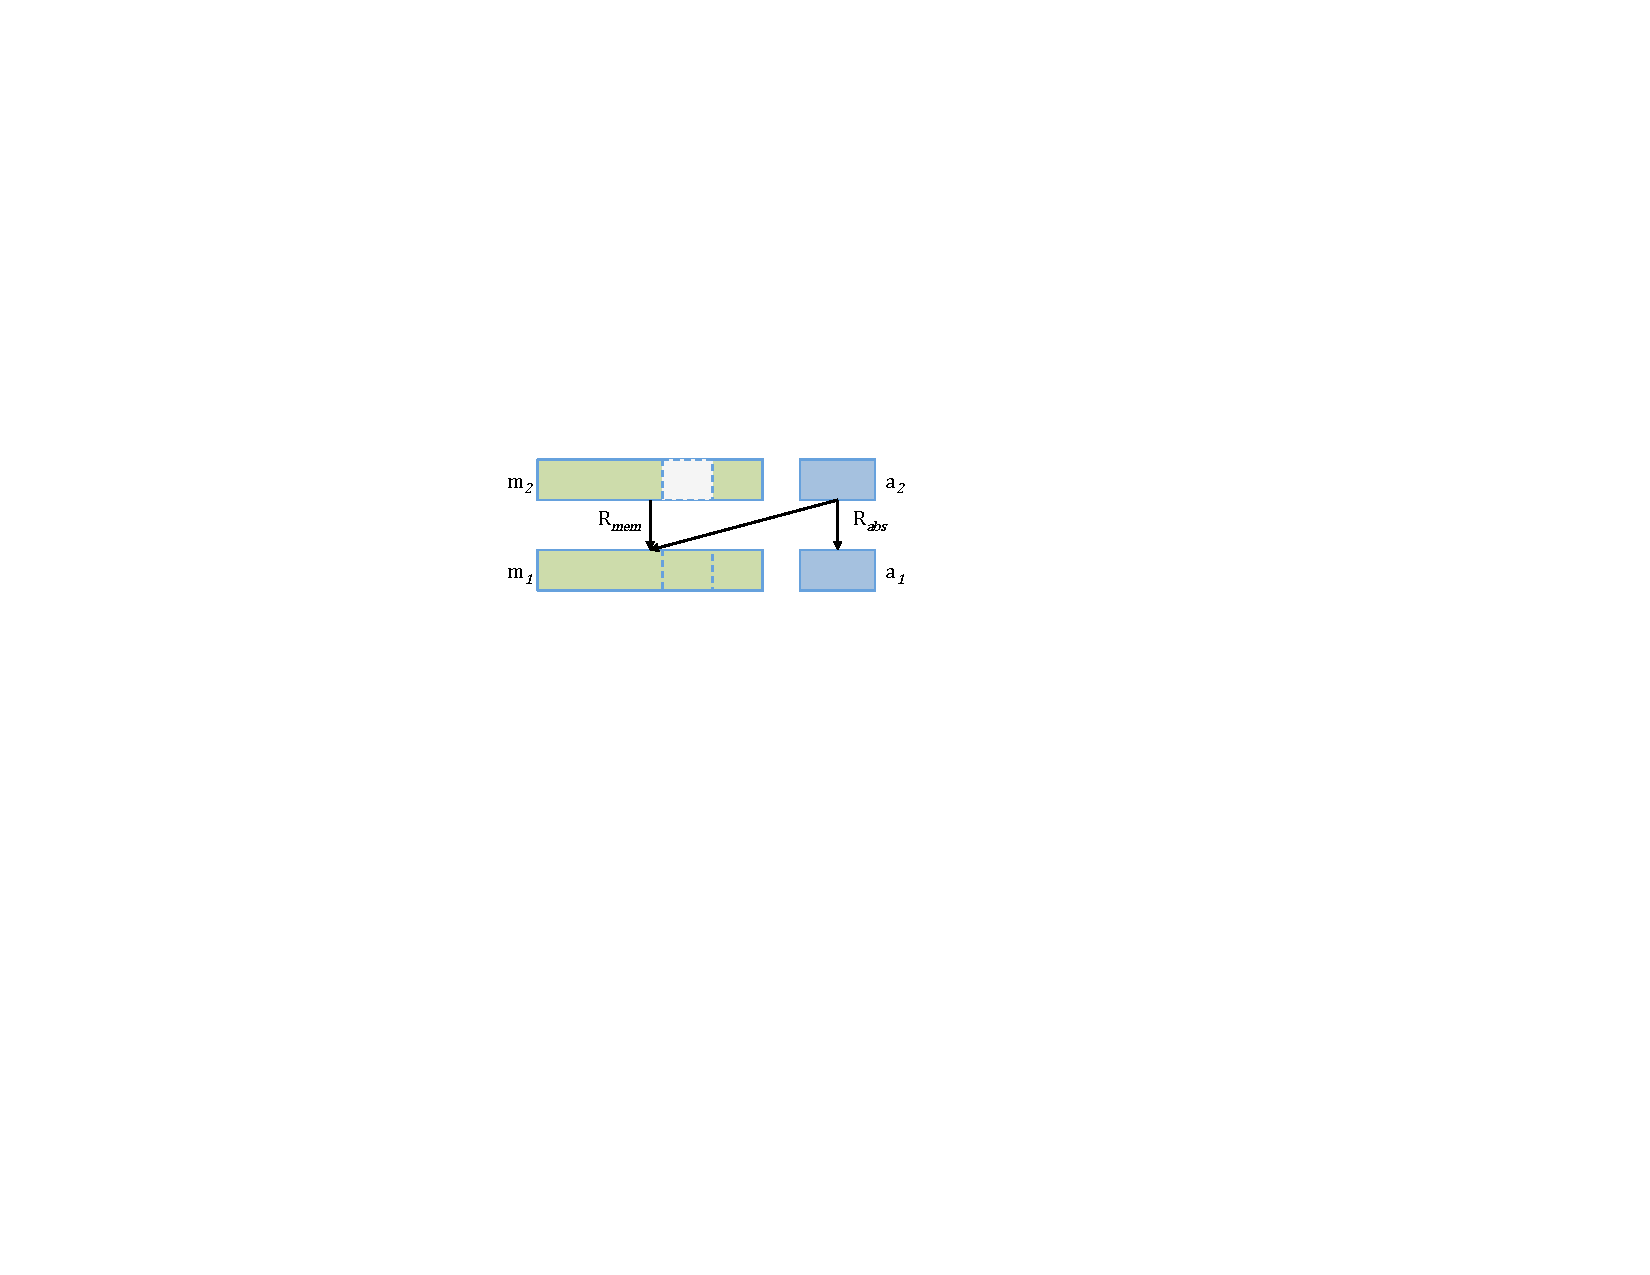
\includegraphics[scale=.7]{figs/layersimulation}
\caption{Layer simulation relation}
\label{fig:layersimulation}
%\vspace*{-7pt}
\end{center}
\afterpage{\FloatBarrier}
\end{figure}

To construct a certified abstraction layer $\layer{L_1}{M}{L_2}$, we
need to find a simulation $R$ such that $\ltyp{L_1}{R}{M}{L_2}$ holds.
Fig.~\ref{fig:lprooftree} gives an overview of this process.  We write
$M = \bigoplus_i i \mapsto \kappa_i$, where $i$ ranges over the
function identifiers defined in module $M$, and $\kappa_i$ is the
corresponding implementation.  Global variables in $M$ should not
be accessible from the layers above: their permissions are removed in
the overlay interface $L_2$.  The interface $L_2$ also includes a
specification $\sigma_i$ for each function $i$ defined in $M$.

We decouple the task of code verification from that of data structure
abstraction. We introduce an intermediate layer interface, $L_1'=\bigoplus_i i \mapsto \sigma'_i$, with its specifications
$\sigma'_i$ expressed in terms of the underlay states.
%%
We first prove that $\ltyp{L_1}{\id}{M}{L_1'}$ holds.  For each
function $i$ in $M$, we show that its implementation $\kappa_i$ is a
downward simulation of its ``underlay'' specification $\sigma'_i$,
that is, $\ltyp{L_1}{\id}{i \mapsto \kappa_i}{i \mapsto
  \sigma'_i}$. We apply the \rulename{Hcomp} rule to compose all the
per-function simulation statements.  Note the simulation
relations here are all \id, meaning there is no abstraction of
data structures in these steps.
%
% This downward simulation can be turned into an upward
% simulation because ClightX is determinate and receptive.  The
% downward simulation proof is sufficient here because the whole
% refinement proof between two layer interfaces is based on downward
% simulation, which will then be turned into an upward simulation at the
% level of whole-machine contextual refinement.
% 
We then prove $L_2 \lpath{R} L_1'$, which means that each specification
$\sigma_i$ in $L_2$ is an abstraction of the intermediate specification
$\sigma'_i$ via a simulation relation $R$.  
From $i \mapsto \sigma_i \lpath{R} i \mapsto \sigma'_i$,  
we apply the monotonicity rule \rulename{LLe-Mon} to 
get $L_2 \lpath{R} L_1'$. Finally, we apply the \rulename{Conseq} rule
to deduce $\ltyp{L_1}{R}{M}{L_2}$. 

%\vspace*{-3pt}
\paragraph{Verifying ClightX functions}
$L_1$ and $L_1'$ share the same views of both concrete and abstract states,
so no simulation relation is involved during this step of verification
(the \rulename{Fun} rule in Sec.~\ref{ssec:layer-langsem}).
Using Coq's tactical language,
we have developed a proof automation engine
that can handle most of the functional correctness proofs of
ClightX programs. It contains two main parts: a ClightX
statement/expression interpreter that generates the verification
conditions by utilizing rules of ClightX big-step semantics,
and an automated theorem prover that discharges
the generated verification conditions on the fly. 
The automated theorem prover is a first order prover,
extended with different theory solvers, such as the theory
of integer arithmetic and the theory of CompCert style partial maps.
The entire automation engine is developed in Coq's Ltac language.


In particular, the arithmetic theory solver is heavily invoked by the
prover. The semantics of Clight requires every value of intermediate
integer expressions to be in the appropriate range of its type. These
expressions may involve regular arithmetic operations such as
addition, subtraction, multiplication and division, but also more
complicated bit-wise operations such as shift, bit-wise and, or, and
complement. The built-in Coq tactic $omega$, which is used to
discharge arithmetic subgoals, is restricted to integer linear
arithmetic formulas, and thus are far from sufficient to deal with
complex formulas in our setting.


%\vspace*{-3pt}
\paragraph{Data abstraction}
Since primitives in $L_1'$ and $L_2$ are atomic, we prove the
single-step downward simulation between $L_1'$ and $L_2$ only at the
specification level.  The simulation proof for the abstraction can be
made language independent.  The simulation relation $R$ captures the
relation between the underlay state (concrete memory and abstract
state) and the overlay state, and can be decomposed as $R_\text{mem}$
and $R_\text{abs}$ (see Fig.~\ref{fig:layersimulation}). The relation
$R_\text{mem}$ ensures that the concrete memory states $m_1$ and $m_2$
contain the same values, while making sure the memory permissions for
the part to be abstracted are erased in the overlay memory $m_2$.  The
component $R_\text{abs}$ relates the overlay abstract state $a_2$ with
the full underlay state $(m_1, a_1)$.

Through this decomposition, we achieve the following two objectives:
the client program can directly manipulate the abstract state without
worrying about its underlying concrete implementation (which is hidden
via $R_\text{mem}$), and the abstract state in the overlay is actually
implementable by the concrete memory and abstract state in the
underlay (via $R_\text{abs}$).

%%%%%%%%%%%%%%%%%%%%%%%%%%%%%%%%%%%%%%%%%%%%
\begin{figure}[t]\scriptsize
$$
\begin{array}{l|l}
\hspace*{-2ex}
\begin{array}[t]{l}
\verb+typedef enum {+\\
\verb+  PG_RESERVED, PG_KERNEL,+\\
\verb+  PG_NORMAL+\\
\verb+} pg_type;+\\
\\
\verb+struct page_info {+\\
\verb+  pg_type	t;+\\
\verb+  uint	u;+\\
\verb+};+\\
\verb+struct page_info AT[1<<20];+
\end{array}
&
\begin{array}[t]{l}
\verb+Notation RESV := 0.+\\
\verb"Notation KERN := (RESV + 1)."\\
\verb"Notation NORM := (KERN + 1)."\\
\\
\verb+Inductive page_info :=+\\
\verb+| ATV (t: Z) (u: Z)+\\ 
\verb+| ATUndef.+\\
\\
\verb+Record abs'' :=+\\
\verb+  {AT: ZMap.t page_info}.+\\
\end{array}
\end{array}
$$ 
\caption{Concrete (C) vs. abstract (Coq) memory allocation table}
\label{fig:alt}
\end{figure}

\begin{figure}[t]\scriptsize
$$
\begin{array}{l|l}
\hspace*{-3ex}
\begin{array}[t]{l}
\verb+// +\kappa_\textsf{at\_get}\\
\verb+uint at_get (uint i){+\\
\verb+  uint allocated;+\\
\verb+  allocated = AT[i].u;+\\
\verb+  if (allocated != 0)+\\
\verb+      allocated = 1;+\\
\verb+  return allocated;+\\
\verb+}+\\
\\
\verb+// +\kappa_\textsf{at\_set}\\
\verb+void at_set (uint i, uint b){+\\
\verb+    AT[i].u = b;+\\
\verb+}+
\end{array}
&
\begin{array}[t]{l}
\verb+Function + \hat{\sigma}_\textsf{at\_get} \verb+ a i :=+\\
\verb+match (a.AT i) with+\\
\verb+| ATV _ 0 => Some 0+\\
\verb+| ATV _ _ => Some 1+\\
\verb+| _ => None+\\
\verb+end.+\\
\\
\verb+Function + \hat{\sigma}_\textsf{at\_set} \verb+ a i b :=+\\
\verb+match (a.AT i) with+\\
\verb+| ATV t _ =>+\\
\verb+Some (set_AT a i (ATV t b))+\\
\verb+| _ => None+\\
\verb+end.+
\end{array}
\end{array}
$$ 
\caption{Concrete vs. abstract getter-setter functions for \textsf{AT}}
\label{fig:alt:gettersetter}
\end{figure}
 
\begin{figure}[t]\scriptsize
$$
\begin{array}{l|l}
\begin{array}[t]{l}
\verb+Inductive +\sigma'_\textsf{at\_set}\verb+ :=+\\
\verb"| "\forall\verb+ m m' a ofs v n,+\\
\verb+   m.store AT ofs v = m'+\\
\verb"  ->"\verb" ofs = n * 8 + 4"\\
\verb"  ->"\verb" 0 <= n < 1048576"\\
\verb"  ->"\verb" "\sigma'_\textsf{at\_set}\verb" (n::v::nil)"\\
\verb"        m a Vundef m' a."
\end{array}
&
\begin{array}[t]{l}
\verb+Inductive +\sigma_\textsf{at\_set}\verb+ :=+\\
\verb"| "\forall\verb+ m a a' n v,+\\
\verb+   +\hat{\sigma}_\textsf{at\_set}\verb+ a n v = Some a'+\\
\verb"  ->"\verb" 0 <= n < 1048576"\\
\verb"  -> "\sigma_\textsf{at\_set} \verb" (n::v::nil)"\\
\verb"       m a Vundef m a'."
\end{array}
\end{array}
$$ 
\caption{High level and low level specification for \textsf{at\_set}}
\label{fig:alt:spec}
\end{figure}

%\vspace*{-3pt}
\paragraph{Common patterns}
We have developed two common design patterns to further ease the task of
verification. The {\it getter-setter} pattern establishes memory
abstraction by introducing new abstract states and erasing
the corresponding memory permissions for the overlay.
The overlay only adds the \textsf{get}
and \textsf{set} primitives which are implemented using simple
memory load/store operations at the underlay.
The {\it abs-fun} pattern implements key functionalities, but does not
introduce new abstract state. Its implementation (on underlay) does
not touch concrete memory state. Instead, it only accesses the states
that have already been abstracted, and it only does
so using the primitives provided by the underlay interface.

Figs.~\ref{fig:alt}-\ref{fig:palloc:spec} show how we use the two
patterns to implement and verify a simplified physical memory
allocator $\textsf{palloc}$, which allocates and returns the
first free entry in the physical memory allocation table.
Fig.~\ref{fig:alt}-\ref{fig:alt:spec} shows how we follow
the {\it getter-setter} pattern
to abstract the allocation table into a new abstract state.
As shown in Fig.~\ref{fig:alt}, we first turn the concrete C
memory allocation table implementation into an abstract Coq data
type. Then we implement the getter and setter functions for the
memory allocation table, both in C and Coq (see Fig.~\ref{fig:alt:gettersetter}). 
The Coq functions $\hat{\sigma}_\textsf{at\_get}$ and $\hat{\sigma}_\textsf{at\_set}$
are just intermediate specifications that are used
later in the overlay specifications.
The actual underlay and overlay specifications of the setter
function $\textsf{at\_set}$ are shown in Fig.~\ref{fig:alt:spec}.

We then prove
$\ltyp{L_1}{\id}{\textsf{at\_set} \mapsto \kappa_\textsf{at\_set}}{\textsf{at\_set} \mapsto \sigma'_\textsf{at\_set}}$,
and also 
$\textsf{at\_set} \mapsto \sigma_\textsf{at\_set}\lpath{R}\textsf{at\_set} \mapsto \sigma'_\textsf{at\_set}$.

\begin{figure}[t]\scriptsize
$$
\begin{array}{l|l}
\hspace*{-3ex}
\begin{array}[t]{l}
\verb+// +\kappa_\textsf{palloc}\\
\verb+uint palloc(uint nps){+\\
\verb+  uint i = 0, u;+\\
\verb+  uint freei = nps;+\\
\verb+  while(freei == nps+\\
\verb+         && i < nps) {+\\
\verb+     u = at_get(i);+\\
\verb+     if (u == 0)+\\
\verb+       freei = i;+\\
\verb"     i ++;"\\
\verb+  }+\\
\verb+  if (freei != nps)+\\
\verb+    at_set(freei, 1);+\\
\verb+  return freei;+\\
\verb+}+\\
\end{array}
&
\begin{array}[t]{l}
\verb+Definition first_free a n:+\\
\verb+  {v| 0<= fst v < n+\\
\verb+   /\+\verb+ a.AT (fst v) = ATV (snd v) 0+\\
\verb+   /\+\verb+ +\forall\ \verb+x, 0 <= x < fst v+\\
\verb+       -> +\sim\verb+a.AT x = ATV _ 0}+\\
\verb"+ {"\forall\ \verb+x, 0 <= x < n+\\
\verb+       -> +\sim\verb+a.AT x = ATV _ 0}.+\\
\\
\verb+Function + \hat{\sigma}_\textsf{palloc} \verb+ a nps :=+\\
\verb+match first_free a nps with+\\
\verb+ | inleft (exist (i, t) _) =>+\\
\verb+   (set_AT a i (ATV t 1), i)+\\
\verb+ | _ => (a, nps)+\\
\verb+end.+\\
\end{array}
\end{array}
$$ 
\caption{Concrete (in C) vs. abstract (in Coq) \textsf{palloc} function}
\label{fig:palloc}
\end{figure}

\begin{figure}[t]\scriptsize
$$
\begin{array}[t]{l}
\verb+Inductive +\sigma'_\textsf{palloc}\verb+ : spec :=+\\
\verb"| "\forall\verb+ m a a' nps n,+\\
\verb+   +\hat{\sigma}_\textsf{palloc}\verb+ a nps = (a', n)+\\
\verb"  -> 0 <= nps < 1048576"\\
\verb"  -> " \sigma'_\textsf{palloc}\verb" (nps::nil) m a n m a'."\\
\\
\verb"Definition "\sigma_\textsf{palloc}\verb" := "\sigma'_\textsf{palloc}.   
\end{array}
$$ 
\caption{High level and low level specification for palloc function}
\label{fig:palloc:spec}
\end{figure}

%%%%%%%%%%%%%%%%%%%%%%%%%%%%%%%%%%%%%%%%%%%%

The code verification (first part) is easy for this pattern
because the memory load and store operations in the underlay
match the source code closely.
The proof can be discharged by our automation tactic.
The main task of this pattern is to prove refinement (second part):
we design a simulation relation $R$
relating the memory storing the global variable at underlay
with its corresponding abstract data at overlay.
The component $R_\text{mem}$ ensures that there is no permission
for allocation table \verb"AT" in overlay memory state $m_2$, 
while the component $R_\text{abs}$ is defined as follows:
\begin{itemize}%[noitemsep,nolistsep]
\item $\forall i \in [0, 2^{20})$, $R_\text{abs}$ enforces the {\em writable}
permission on \verb"AT[i]" at underlay memory state $m_1$, and requires
($a_2$.\verb"AT"  \verb"i") at overlay to be
\verb"(ATV AT[i].t AT[i].u)".

\item Except for \verb"AT", $R_\text{abs}$ requires all other abstract data in
underlay and overlay to be the same.
\end{itemize}
The refinement proof for $L_2 \lpath{R} L_1'$ involves the efforts to
prove that this relation $R$ between underlay memory and overlay
abstract state is preserved by all the atomic primitives in both $L_1'$ and $L_2$.

After we abstract the memory and get/set operations,
%of the allocation table
we implement $\textsf{palloc}$ on top of $L_2$,
following the {\it abs-fun} pattern.
The previous overlay now becomes the new underlay (``$L_1$'').
Fig.~\ref{fig:palloc} shows both the implementation of
$\textsf{palloc}$ in ClightX and the abstract function in Coq.
As before, we separately show that
$\ltyp{L_1}{\id}%
	{\textsf{palloc} \mapsto \kappa_\textsf{palloc}}%
	{\textsf{palloc} \mapsto \sigma'_\textsf{palloc}}$,
and 
$\textsf{palloc} \mapsto \sigma_\textsf{palloc}\lpath{R}
\textsf{palloc} \mapsto \sigma'_\textsf{palloc}$
holds.
For the {\it abs-fun} pattern, the refinement proof is easy.
Since we do not introduce any new abstract states in this pattern,
the implementation only manipulates the abstract states through the
primitive calls of the underlay. Thus, as shown in Fig. \ref{fig:palloc:spec},
the corresponding underlay and overlay specifications are exactly the same,
so the relation $R$ here is the identity (\id) and 
the proof of refinement is trivial.
The main task for the {\it abs-fun}
pattern is to verify the code, which is done using our automation tactic. 


Due to the presence of a loop in the C code (see Fig.~\ref{fig:palloc}), 
the automation tactic is not able to automate the proofs completely.
Since the big-step semantics only specifies the infinite loop,
naive applications of the semantic constructors of loops as
logical rules lead to an infinite sequence of applications.
In our framework, we introduce a separate inference rule as a
lemma for proving both the correctness and the termination of the loops.
The lemma requires the prover to provide both the loop invariants
(for partial correctness) and the loop variant (for termination).
Once the right loop invariants and variant are provided, the proof
can be mostly automated using our proof automation engine.


The above examples show that for the {\it getter-setter} pattern, the
primary task is to prove data abstraction, while for the {\it abs-fun}
pattern, the main task is to do simple program verification.  These
two tasks are well understood and manageable, so the decoupling (via
these two patterns) makes the layer construction much easier. 


It means that although
the proof of $\ltyp{L_1}{R}{M}{L_2}$ is separated into two disjoint
tasks, by following the two patterns, the proof is merely focused
on one of them.



\paragraph{Verification of Functional Correctness}

Verification of ClightX code is done on a per-function basis.
For each function $f$ implemented on top of layer interface $L$, we write a deep specification
$f_S$ of the form $f_S(args,m,a,res, m',a')$, which precisely capture
the change of states by $f$ from $(m, a)$ into $(m', a')$ with
return value $res$ when executed with arguments $args$.
Then we prove a downward simulation relation between $f_S$ and $f$,
which can be turned into the upward simulation, i.e., the proof
that the implementation is the refinement of the specification,
due to the fact that the semantics of the $ClightX(L)$ is deterministic.
However, the downward simulation proof is enough in our case,
in the sense that we do not need to turn downward simulation into upward simulation,
because the whole refinement proof between two layer interfaces is based on downward simulation,
which is in turn turned into an upward simulation at the level of whole-machine contextual
refinement.

For example, show dequeue refinement theorem here...

To prove the above theorem, we have developed a powerful proof automation
engine for the language ClightX, all in Coq's tactical language.
It directly utilizes the constructors of the CompCert ClightX big-step
semantic rules to interpret the statements of the function body, while
using it's back-end theorem proving engines to automatically discharge
the verification conditions generated by applying the semantic constructors.

Talk about the verification condition generation here...

Talk about the tautology solver, advanced arithmetic theory solver, term rewritter and so on...

This is possible thanks to the analogy between the deep specification and the concrete
implementation.



\paragraph{Establishing Invariants}
Global variables usually require stating and proving some invariant properties.
For example, in operating system design, thread queues are normally implemented
as doubly-linked lists. The corresponding invariants might state that,
\begin{invariant}
\begin{enumerate}
\item The queue is well formed, i.e., all forward and back links in the list
point to the appropriate node (except the head and tail).
\item Non-active threads are not in any of the thread queue.
\item All active threads appear in one and exactly one thread queue.
\item Each thread can appear in a queue at most once.
\item Each queue only contains active threads.
\end{enumerate}
\end{invariant}
Invariants are expensive because they need to be proved not only
locally for the functions manipulating the variables, but also for the whole system,
e.g., need to show that no other pointer manipulations in the system
destroy the invariant properties. 
In other words, invariants are the global properties that are expected to hold
in any execution of the program.
Furthermore, sometimes, some functions have
to temporarily break the invariants. For example, the \verb+dequeue+ operator,
which removes a node from the doubly linked list, temporarily breaks the invariants
by allowing the queue to be temporarily ill formed in the middle of execution.
In complex systems like operating system kernel, proofs on invariants are even
trickier, as you not only need to show the invariants hold on the kernel implementation,
but also during the execution of any client/user programs.
For the seL4 project, though they prove the properties of kernel source code alone,
they mention that 80\% of their initial efforts in the
refinement proofs went into establishing invariants, and only 20\% into the
actual functional correctness proof \cite{klein2009sel4}.

In the verification of the \mCTOS{} (see Section \ref{sec:kernel}),
we take a novel approach, which we believe significantly eased the task of invariant
related proofs. 
First, we never enforce any explicit invariants on the raw memory. All the kernel data
structures in the memory are first abstracted into logical states. And all the
invariants are stated in terms of those abstract data. Recall the only way
a ClightX program interacts with abstract data is by calling the primitives.
At each layer interface $L$, we state the invariants $inv(L)$ strictly on the abstract
data of $L$, and show a global property that the invariants hold at any execution
point of any programs running on $L$. This is achieved by showing the initial
abstract data satisfies the invariants, and all the primitives of $L$ preserve
the invariants of $L$. 
Thanks to this global property, during a verification of the functional correctness
of function $f$ implemented on top of layer interface $L$, you get free access to use all the invariants
of $L$ as facts. It also exempt you completely from worrying about invariants
related proofs during the proof of functional correctness of $f$.
During the verification of $f$, there is no need
to prove anything related to invariant preservation, cause it is already proved globally
that whatever the function does, the invariants are preserved.

The function $f$ verified on top of the underlay $L$ may get exposed as an abstract primitive to
the overlay. The overlay may have a completely different set of layer invariants,
and you just need to prove that the abstract specification of the function preservers
the invariants of the overlay, to achieve the global invariants property of the
overlay.
For example, you may implement a setter/getter on top of underlay $L$, which reads and writes to
a piece of memory. We do not enforce any invariants on that piece of memory. At the
overlay, that memory is abstracted into an abstract data type, and we show that
the abstract specifications of setters and getters (which reads and writes to the
abstract states instead), preserve the invariants of that overlay.

This new approach has following advantages:
\begin{itemize}
\item For each layer interface $L$, invariant proofs are done globally once and for all.
This let us focus on the main functional correctness proofs.
\item Invariant preservation proofs are always on abstract specifications, which
are atomic. You no longer need to worry about the actual implementation of the
function temporarily breaks the invariants in the middle of the execution.
\item Postpone the introduction of invariants to the right layer interface.
We introduce the last 4 invariants of the thread queue implementation above
only when we get to the most abstract view shown in the Example ?.
This means, those invariants are no longer proved on complicated initial or
intermediate representations of the thread queues, but only proved with
the most abstract specifications, where a thread queue is interpreted as a
Coq list.
\item Better isolation. The invariants on abstract data that is not modified
by an abstract specification is trivially satisfied.
\item Hiding primitives. The second invariants above can easily be violated
if you simply call a primitive to inactivate or free a thread in a queue
before popping the queue out of the thread. But when we introduce the
invariants we hide the corresponding low level primitives that directly
activates/deactivates threads, enqueue, dequeue, and expose a more higher
level primitive \verb+thread_free+, which both deactivates a thread and
pops the thread out of the queue. Since the primitive execution is atomic,
this does not break any invariants of the layer interface. In a word, when we introduce
new invariants that potentially get broken by previous low level primitives,
we implement and expose only new high level primitives that respects the
invariants. This restricts the context program to only those that respects
our invariants.
\item Hiding the invariants. Once the virtual memory manager is implemented,
there is no need to expose the low level physical memory allocation table
any more to the overlay or the higher layers. When we hide the corresponding abstract
data and primitives, we also remove corresponding invariants on the data
as well. Fewer number of invariants means fewer proof efforts needed.
\end{itemize}




\begin{figure}[t]\scriptsize
$$
\begin{array}{l}
\begin{array}{l}
\verb+struct pmap {+\\
\verb+  alignas(4096) uint pdir[1024];+\\
\verb+  alignas(4096) uint pt[1024][1024];+\\
\verb+};+\\
\verb+alignas(4096) struct pmap pmp[64];+\\
\\
\verb+void set_PTX(uint pid, uint pde, uint pte,+\\
\verb+             uint paddr, uint perm){+\\
\verb"  pmp[pid].pt[pdx][ptx] = paddr + perm;"\\
\verb+}+
\end{array}
\\
\hline
\\
\begin{array}{l}
\verb+Inductive PTPerm: Type := |PTE_P |PTE_W |PTE_U.+\\
\verb+Inductive PTInfo:=+\\
\verb+  |PTValid (v: block)(p: PTPerm) |PTUnPresent |PTUndef.+\\
\verb+Definition pt := ZMap.t PTInfo.+\\
\verb+Inductive pdir := |PDTValid (pte: pt) |PDTUndef.+\\
\verb+Definition pmap := ZMap.t pdir.+\\
\verb+Definition pmp := ZMap.t pmap.+
\end{array}
\end{array}
$$ 
\caption{Concrete (in C) vs. abstract (in Coq) page maps}
\label{fig:pmap}
%\vspace*{-7pt}
\end{figure}



\section{Layered Programming in LAsm}
\label{sec:seq:lasm}

In this section, we describe LAsm, the \emph{Layered
  Assembly language}, and the extended machine model which LAsm is based on.

The reason we are interested in assembly code and behavior is
threefold.  First of all, even though we provide ClightX to write most
code, we are still interested in the actual assembly code running on
the actual machine. In Section \ref{sec:seq:comp}, we will provide a
verified compiler to transport all proofs of code written in ClightX
to assembly.

\begin{figure}[t]\centering
\lstinputlisting [language = C, multicols=2] {source_code/seq-cswitch.c}
\caption{Kernel context switch verified in LAsm}
\label{fig:contextswitch}
\hrulefill
\end{figure}

Secondly, there are parts of software that have to be manually written
in assembly for various reasons. For example, the standard
implementation of kernel context switch, shown in
Figure~\ref{fig:contextswitch}, 
modifies the stack pointer register
\textsf{ESP}, which does not satisfy the C calling convention and has
to be verified in assembly.  A linker will be defined in Section
\ref{sec:seq:comp} to link them with compiled C code.

Last but not least, we are interested not only in the behavior of our
code, but also in the behavior of the \emph{context} that will call
functions defined in our code. To be as general as possible, we allow
the context to include all valid assembly code sequences. To this end,
it is necessary to transport per-function refinement proofs to a
whole-machine \emph{contextual refinement} proof.


  \subsection{LAsm and layer interfaces}

We start from the syntax and formal semantics of the 32-bit x86
assembly subset specified in CompCert.
CompCert x86 assembly is
modeled as a state machine with a register set and a memory state. 
The register set
consists of eight 32-bit general-purpose registers and eight XMM registers
designated as scalar double-precision floating-point operands.
The memory state is same as the one in Clight.
In particular, each function executes with its stack frame modeled in its
own memory block, so that the stack is not a contiguous piece of
memory.
Another anomaly regarding function calls in CompCert x86 assembly is that
the return address is stored in pseudo-register $\mathsf{RA}$ instead of
being pushed onto the stack, so
that the callee must allocate its own stack frame and
store the return address 
using the \textsf{Pallocframe} and
\textsf{Pfreeframe} pseudo-instructions.

\begin{figure}[t]\centering
\[
\begin{array}{llll}
\mathit{ri}  & ::= & \mathsf{ESP} \, | \mathsf{EBP} \, & \text{Stack registers} \\
& | & \mathsf{EAX} \, | \mathsf{EBX} \, | \mathsf{ECX} \, | \mathsf{EDX} & \text{Integer registers} \\
\mathit{rf} & ::= & \mathsf{FP0} \, | \mathsf{XMM0} \, | \mathsf{XMM1} \dots | \mathsf{XMM7} & \text{Floating-point registers} \\
r & \in & \textsf{preg} & \text{Registers} \\
 & ::= & \mathit{ri} \, | \mathit{rf} \\
& | & \mathsf{EIP} \, | \mathsf{RA} & \text{Prog counter, return addr} \\
\end{array}
\]
\[
\begin{array}{llll}
\mathit{ti} & ::= & \mathit{ri} & \text{Direct integer register access} \\
& | & (\mathit{ri})n & \text{Indirect load/store via int register} \\
& | & x+n & \text{Load/store to global variable} \\
\mathit{si} & ::= & \mathit{ti} & \text{Dereference} \\
& | & \$n & \text{Constant integer} \\
& | & \$x+n & \text{Pointer to global variable} \\
\\
\mathit{tf} & ::= & \mathit{rf} \, | (\mathit{ri})n \, | x+n & \text{Floating-point targets} \\
\mathit{sf} & ::= & \mathit{tf} \, | \$q \, & \text{Floating-point sources} \\
\\
\mathit{I} & ::= & \mathtt{movi} ~ \mathit{si}, \mathit{ti} & \text{Integer move/load/store} \\
& | & \mathtt{leai} ~ \mathit{si}, \mathit{ti} & \text{Integer load/store from address} \\
& | & \mathtt{movf} ~ \mathit{sf}, \mathit{tf} & \text{Floating-point move/load/store} \\
& | & \mathtt{addi} ~ \mathit{ri}_d, \mathit{ri}_o & \text{Arithmetic} \\
& | & \mathtt{subi} ~ \mathit{ri}_d, \mathit{ri}_o \, | \dots \\
& | & \mathtt{call} ~ \mathit{ti} \, | \mathtt{ret} & \text{Function call and return} \\
& | & \mathtt{push} ~ \mathit{ri} \, | \mathtt{pop} ~ \mathit{ri} & \text{Regular register push/pop} \\
& | & \mathsf{Pallocframe} ~ n & \text{Allocate stack frame} \\
& | & \mathsf{Pfreeframe} ~ n & \text{Free stack frame}
\end{array}
\]
\caption{The syntax of LAsm}
\label{fig:seq:lasm:syntax}
\hrulefill
\end{figure}

Similarly to ClightX, we extend the machine state with an abstract
state, which will be modified by primitives. This yields LAsm, whose
syntax (\cf Figure~\ref{fig:seq:lasm:syntax}) is the same as that of CompCert x86 assembly, except that the
semantics will be parameterized over the type of abstract states and
the specifications of primitives.  Most notably, primitive calls are
syntactically indistinguishable from normal function calls, yet depend
on the specifications semantically.

Moreover, in our Coq formalization, the semantics of LAsm is also
equipped with \emph{memory accessors} for address translation in order to handle both
kernel memory linear mapping and user space virtual memory.
In the latter case, plain integers can be treated
as pointers to user memory, as opposed to kernel memory modeled as the
CompCert-style concrete memory state. 

\begin{definition}[LAsm Modules]
A LAsm module is a finite map from identifiers to arrays of LAsm
instructions.
\end{definition}

\ignore{We define the semantics of LAsm in small-step form. The machine
state is $(\rho, m, a)$ where $\rho$ contains the values of registers,
$m$ is the concrete memory state and $a$ is the abstract state. Let
$M$ be an LAsm module, which is a finite map from identifiers to arrays of LAsm
instructions, we write $\Gamma, L, M \vdash (\rho, m, a)
\rightarrow (\rho', m', a')$ a transition step in the LAsm machine. The full syntax and formal semantics of LAsm is described in the
  companion technical report.}

\ignore{
\begin{figure}[t]\scriptsize
$$
\begin{array}{l|l}
\begin{array}{l}
\verb+kctxt_switch:+\\
\verb+	leai	0(%eax,%eax,2), %eax+\\
\verb+	leai	KCtxtP(,%eax,8), %eax+\\
\verb+	movi	%esp, 0(%eax)+\\
\verb+	movi	%edi, 4(%eax)+\\
\verb+	movi	%esi, 8(%eax)+\\
\verb+	movi	%ebx, 12(%eax)+\\
\verb+	movi	%ebp, 16(%eax)+\\
\verb+	pop	%ecx+\\
\verb+	movi	%ecx, 20(%eax)+\\
\verb+	leai	0(%edx,%edx,2), %edx+
\end{array}
&
\begin{array}{l}
\\
\verb+	leai	KCtxtP(,%edx,8), %edx+\\
\verb+	movi	0(%edx), %esp+\\
\verb+	movi	4(%edx), %edi+\\
\verb+	movi	8(%edx), %esi+\\
\verb+	movi	12(%edx), %ebx+\\
\verb+	movi	16(%edx), %ebp+\\
\verb+	movi	20(%edx), %ecx+\\
\verb+	push	%ecx+\\
\verb+	xor	%eax, %eax+\\
\verb+	ret+\\
\verb+......+
\end{array}
\end{array}
$$
\caption{Kernel context switch verified in LAsm}
\label{fig:contextswitch}
\end{figure}
}

%\vspace*{-3pt}
\paragraph{Assembly layer interfaces}
The semantics of LAsm is parameterized over a layer interface.
Different from C-style primitives (\cf Definition~\ref{def:c-prim}), which are defined using
argument list and return value, primitives implemented in LAsm
often utilize their full control over the
register set and are not restricted to a particular calling convention (\eg, context switch).
Therefore, it is necessary to extend the structure of layer
interfaces to allow assembly-style primitives modifying the register set.

\begin{definition}[Assembly-style primitive]
An assembly-style primitive specification $P$ over the abstract state type
$\abst$ is a predicate on $((\textsf{preg} \rightarrow \textsf{val}) \times \textsf{mem} \times \abst) \times
((\textsf{preg} \rightarrow \textsf{val}) \times \textsf{mem} \times \abst)$. $P(\rho, m, a,
\rho', m', a')$ says that the primitive $P$ takes
register set $\rho$, memory state $m$ and abstract state $a$ as
arguments, and returns register set $\rho'$, memory state
$m'$ and abstract state $a'$ as result.
\end{definition}

By ``\emph{style},'' we mean the calling convention,
not the language in which they are actually implemented.
C-style primitives may very well be implemented as hand-written
assembly code at underlay.

We can then define assembly layer interfaces by replacing the primitive
specification with our assembly-style one in Definition~\ref{def:c-layer}.
But, to make reasoning simpler, when defining assembly layer interfaces,
we distinguish C-style from assembly-style primitives.
First, C-style primitives
can be refined by other C-style primitives. 
Second and most importantly, it
becomes possible to instantiate the semantics of ClightX with an
\emph{assembly} layer interface by just considering C-style primitives and ignoring
assembly-style primitives (which might not follow the C calling convention).
In this way, ClightX code is only allowed to call C-style
primitives, whereas LAsm can actually call both kinds of primitives.

\begin{definition}[Assembly layer interface] \label{def:asm-layer}
An assembly layer interface $L$ is a tuple
$ L = (\abst, \primt_{\mathrm{ClightX}}, \primt_{\mathrm{LAsm}}, \invt, \mat) $
where:
\begin{itemize}
\item $(\abst, \primt_{\mathrm{ClightX}}, \invt)$ is a C layer interface (\cf
Definition~\ref{def:c-layer})
\item $\primt_{\mathrm{LAsm}}$ is a finite map from identifiers to assembly-style
primitive specifications over the abstract state $\abst$. The domains of
$\primt_{\mathrm{ClightX}}$ and $\primt_{\mathrm{LAsm}}$ shall be disjoint.
\item $\mat$ is the memory accessor used for address translation.
\end{itemize}
\end{definition}


\paragraph{Small-step semantics}

We write $\llbracket \mathit{ti} \rrbracket^\triangleleft(\Gamma, \rho)$
(\emph{resp}. $\llbracket \mathit{tf} \rrbracket^\triangleleft(\Gamma, \rho)$)
to denote the evaluation of integer (\emph{resp}. floating-point) registers
and global variables as targets for \texttt{mov} operations, where
$\Gamma$ is a mapping from global variables to memory block
identifiers, and $\rho$ is a mapping from registers to values.

\[
\begin{array}{lll}
\llbracket (\mathit{ri})n \rrbracket^\triangleleft(\Gamma, \rho) & = (n' + n) & \text{if} ~ \rho(\mathit{ri}) = n' \\
\llbracket (\mathit{ri})n \rrbracket^\triangleleft(\Gamma, \rho) & = (b, \mathit{ofs}+n) & \text{if} ~ \rho(\mathit{ri}) = (b, \mathit{ofs}) \\
\llbracket x + n  \rrbracket^\triangleleft(\Gamma, \rho) & = (b, n) & \text{if} ~ \Gamma(x) = b
\end{array}
\]

To evaluate indirect load through registers and global variables as
source operand for $\mathtt{mov}$ operations, we write $\llbracket s
\rrbracket^\triangleright(\Gamma, \rho, m)$ the evaluation of
\texttt{mov} operands.

\[
\begin{array}{ll}
\llbracket s \rrbracket^\triangleright(\Gamma, \rho, m)  = m(v) &
\text{if }  \llbracket s \rrbracket^\triangleleft(\Gamma, \rho) = v 
\\
\llbracket r \rrbracket^\triangleright(\Gamma, \rho, m)= \rho(r) &
\llbracket \$ n \rrbracket^\triangleright(\Gamma, \rho, m)  = n 
\\
\llbracket \$ q \rrbracket^\triangleright(\Gamma, \rho, m)  = q 
\\
\llbracket \$ x+n \rrbracket^\triangleright(\Gamma, \rho, m)  = (b, n)  &
\text{if }  \Gamma(x)  = b 
\end{array}
\]

For any register set $\rho$, we write 
\[\mathsf{nextEIP}(\rho) =
\rho[\mathsf{EIP} \leftarrow (b, \mathit{ofs}+1)] \text{ if }\rho(\mathsf{EIP})
  = (b, \mathit{ofs})\]%
The register $\mathsf{EIP}$ is assumed to contain a
  pointer $(b, \mathit{ofs})$ where $b$ is the memory block
  corresponding to the current function, and $\mathit{ofs}$ is the
  index of the current instruction within this function; in the exact
  same way as in CompCert x86 assembly, we assume that all
  instructions are of size 1.

Function call and return only modify the value of registers \textsf{EIP} and \textsf{RA}.

Similarly to CompCert x86 assembly, \textsf{Pallocframe} allocates a
new stack frame memory block, stores the return address and a back
link to the parent stack frame, and makes the stack pointer point to
the new stack frame. Conversely, \textsf{Pfreeframe} restores the
previous values of the stack pointer and return address, then frees
the current stack block.

We define the semantics of LAsm in small-step form. The machine
state is $(\rho, m, a)$ where $\rho$ contains the values of registers,
$m$ is the concrete memory state and $a$ is the abstract state.  Let
$M$ be a module, we write $\Gamma, L, M \vdash (\rho, m, a)
\rightarrow (\rho', m', a')$ a transition step in the LAsm machine.

\begin{figure}[t]
\begin{mathpar}
\inferrule{
\llbracket s \rrbracket ^ \triangleright(\Gamma, \rho, m)  = v 
\\
\rho'  = \mathsf{nextEIP}(\rho[r \leftarrow v])
}
{\llbracket \mathtt{mov}~ s, r \rrbracket(\Gamma, L; \rho, m, a)  = (\rho', m, a)}
\and
\inferrule{
\llbracket s \rrbracket ^ \triangleright(\Gamma, \rho, m) = v_s
\\
\llbracket t \rrbracket ^ \triangleleft(\Gamma, \rho) = v_t\\
m' = m[v_t \leftarrow v_s]\\
\rho_2  = \mathsf{nextEIP}(\rho_1)
}
{\llbracket \mathtt{mov}~ s, t \rrbracket(\Gamma, L; \rho, m, a) = (\rho_2, m', a') }
\and
\inferrule{
\rho(r_s)  = n 
\\
\rho(r_t) = (b, \mathit{ofs}) 
\\
\rho' = \mathsf{nextEIP}(\rho[r_t \leftarrow (b, \mathit{ofs}+n)])
}
{\llbracket \mathtt{addi}~ r_s, r_t \rrbracket(\Gamma, L; \rho, m, a) = (\rho', m, a) }
\and
\inferrule{
\rho(r_s) = (b, \mathit{ofs}_s) 
\\
\rho(r_t) = (b, \mathit{ofs}_t) 
\\
\rho' = \mathsf{nextEIP}(\rho[r_t \leftarrow (\mathit{ofs}_t - \mathit{ofs}_s)])
}
{\llbracket \mathtt{subi}~ r_s, r_t \rrbracket(\Gamma, L; \rho, m, a) = (\rho', m, a) }
\and
\inferrule{
\llbracket t \rrbracket^\triangleleft(\Gamma, \rho)  = v
\\
\rho' = \rho[\mathsf{EIP} \leftarrow v][\mathsf{RA} \leftarrow \rho(\mathsf{EIP})] 
}
{\llbracket \mathtt{call} ~ t \rrbracket(\Gamma, L; \rho, m, a) = (\rho', m, a)}
\and
\inferrule{
\rho' = \rho[\mathsf{EIP} \leftarrow \rho(\mathsf{RA})][\mathsf{RA} \leftarrow \bot]
}
{\llbracket \mathtt{ret} \rrbracket(\Gamma, L; \rho, m, a) = (\rho', m, a) }
\and
\inferrule{
m_1  = \mathsf{alloc}(n)(m) 
\\
m_2  = m_1[(\mathsf{next}(m), 0) \leftarrow \rho(\mathsf{RA})]
\\
m' = m_2[(\mathsf{next}(m), 4) \leftarrow \rho(\mathsf{ESP})]
\\
\rho' = \rho[\mathsf{ESP} \leftarrow (\mathsf{next}(m), 0)]
}
{\llbracket \mathsf{Pallocframe} ~ n \rrbracket(\Gamma, L; \rho, m, a) = (\rho', m', a) }
\and
\inferrule{
\rho(\mathsf{ESP})  = (b, 0)
\\
m(b, 0) = \mathit{ra}
\\
m(b, 4) = \mathit{esp}
\\
m' = \mathsf{free}(b, n)(m)
\\
\rho'  = \rho[\mathsf{ESP} \leftarrow \mathit{esp}][\mathsf{RA} \leftarrow \mathit{ra}] 
}
{\llbracket \mathsf{Pfreeframe} ~ n \rrbracket(\Gamma, L; \rho, m, a) = (\rho', m', a)}
\end{mathpar}
\caption{Execution step of LAsm instructions}
\label{fig:seq:lasm:sem}
\hrulefill
\end{figure}


For any instruction $I$, we write $\llbracket I \rrbracket (\Gamma, L;
\rho, m, a) = (\rho', m', a')$ for its execution step.
For the sake of presentation, in Figure~\ref{fig:seq:lasm:sem},
we only show a simplified version of
the execution step of LAsm instructions,
where memory accesses only use the CompCert-style kernel memory (\ie, the address translation is an identity function). 
\ronghui{FIx}

For an internal function, we look into the module for the
instruction to execute.
\[
\inferrule{
  \rho(\mathsf{EIP}) = (b, \mathit{ofs}) \\
  \Gamma(f) = b \\
  M(b)(\mathit{ofs}) = I \\
  \llbracket I \rrbracket (\Gamma, L; \rho, m, a) = \rho', m', a'
}{
  \Gamma, L, M \vdash (\rho, m, a) \rightarrow (\rho', m', a')
}
\]

For external function calls, there are two cases, one for the case of
assembly-style primitives, and the other for the case of the C-style primitives.

For assembly-style primitives, we directly take the step from the
specification of the primitive in $L$.
\[
\inferrule{
  \rho(\mathsf{EIP}) = (b, 0) \\
  \Gamma(f) = b \\
  \Gamma \vdash L.\primt_{\mathrm{LAsm}}(f)(\rho, m, a, \rho', m', a')
}{
  \Gamma, L, M \vdash (\rho, m, a) \rightarrow (\rho', m', a')
}
\]

For C-style primitives, we take the specification of the primitive
from the C-style primitive component of $L$, but we have to wrap it into the
calling convention. We write $\mathsf{arguments}(\mathit{args}, m, v)$
to denote the fact that the arguments are stored in memory $m$, at the
stack pointer $v$; for primitives returning integer or
pointer values, we store the value to the \texttt{EAX} register. We
write $\mathsf{eraseNonCalleeSave}(\rho)$ to set to $\bot$ the
contents of all non-callee-save registers in $\rho$.
\[
\inferrule{
  \rho(\mathsf{EIP}) = (b, 0) \\
  \Gamma(f) = b \\
 \Gamma \vdash L.\primt_{\mathrm{ClightX}}(f)(\mathit{args}, m, a, \mathit{res}, m', a') \\
  \rho(\mathsf{ESP}) \neq \bot \\
  \mathsf{arguments}(\mathit{args}, m, \rho(\mathsf{ESP})) \\
  \rho(\mathsf{RA}) \neq \bot \\
  \rho' = \mathsf{eraseNonCalleeSave}(\rho)[\mathsf{EAX} \leftarrow \mathit{res}][\mathsf{EIP} \leftarrow \rho(\mathsf{RA})][\mathsf{RA} \leftarrow \bot]
}{
  \Gamma, L, M \vdash (\rho, m, a) \rightarrow (\rho', m', a')
}
\]


\paragraph{Whole-machine semantics and contextual refinement}

Based on the relational transition system which we just defined for LAsm,
we can define the whole-machine semantics including not only the code
that we wrote by hand or that we compile, but also the \emph{context}
code that shall call our functions. To this end, it suffices to equip
the semantics with a notion of initial and final state, in a way
similar to the CompCert x86 whole-program assembly semantics.

In CompCert, the initial state consists of an empty register set
with only \textsf{EIP} (instruction pointer register) pointing to the \texttt{main} function of the
module, and the memory state is constructed by allocating a memory
block for each global variable of the program. We follow the same
approach for LAsm, except that we also need an initial abstract
state, provided by the layer interface, so
we need to extend its definition:

\begin{definition}[Whole-machine layer interface] \label{def:whole-machine-layer}
A whole-machine layer interface $L$ is a tuple
$L = (\abst, \primt_{\mathrm{ClightX}}, \primt_{\mathrm{LAsm}}, \invt, \mat, a_0)$
where:
\begin{itemize}
\item $ (\abst, \primt_{\mathrm{ClightX}}, \primt_{\mathrm{LAsm}}, \invt, \mat) $ is an assembly layer interface
\item $a_0 : A$ is the initial abstract state.
\end{itemize}
\end{definition}

\begin{definition}[Whole-machine initial state]
The whole-machine LAsm initial state for layer $L$ and module $M$ is
the LAsm state $(\rho_0, m_0, a_0)$ defined as follows:
\begin{itemize}
\item $\rho_0(r) = \left\{ \begin{array}{ll}
(\Gamma(\mathtt{main}), 0) & \text{if} ~ r = \mathsf{EIP} \\
%\ifTR{0 & \text{if} ~ r = \mathsf{RA} \\}{}
0 & \text{if} ~ r = \mathsf{RA} \\
\bot & \text{otherwise}
\end{array}
\right. $
\item $m_0$ is constructed from the global variables of $\Gamma, L, M$
\item $a_0$ is the whole-machine initial state specified in $L$
\end{itemize}
\end{definition}

\begin{definition}[Whole-machine final state]
A whole-machine LAsm state $(\rho, m, a)$ is final with return code
$n$ if, and only if, $\rho(\mathsf{EAX}) = n$ and $\rho(\mathsf{EIP}) =
0$.
\end{definition}

Notice that $\rho(\mathsf{EIP})$ contains the \emph{integer} 0,
which is also the initial return address and is not a valid pointer.
This ensures that executions do not
go beyond a final state, following the CompCert x86 whole-program
semantics: \texttt{main} has returned to its ``caller'', which does
not exist. Thus, the final state is uniquely determined (there can be
no other possible behavior once such a state is reached), so the
whole-machine semantics is deterministic once the primitives are.

\begin{definition}[Whole-machine behavior]
Let $\Gamma$ be a mapping of global variables to memory blocks. Then, we say that
\begin{itemize}
\item $\mathit{LAsm}(\Gamma, L, M)$ \emph{diverges} if there is an
  infinite execution sequence from the whole-machine initial state for $L$
\item $\mathit{LAsm}(\Gamma, L, M)$ \emph{terminates with return code} $n$ if there is a finite execution sequence from the whole-machine initial state for $L$ to a whole-machine final state with return code $n$
\item $\mathit{LAsm}(\Gamma, L, M)$ \emph{goes wrong} if there is a finite execution sequence from the whole-machine initial state for $L$ to a non-final state that can take no step.
\end{itemize}
$M$ is said to be \emph{unsafe} in layer interface $L$ if $\mathit{LAsm}(\Gamma, L, M)$ goes wrong.
\ignore{
\tahina {TODO: should we also have traces?}
}
\end{definition}

Then, we are interested in \emph{refinement} between whole machines:
\begin{definition}[Whole-machine refinement]
Let $L_{\text{high}}, L_{\text{low}}$ be two whole-machine assembly
layer interfaces, and $M_{\text{high}}, M_{\text{low}}$ be two LAsm
modules. Then, we say that $M_{\text{low}} @ L_{\text{low}}$ refines
$M_{\text{high}} @ L_{\text{high}}$, and write $M_{\text{low}} @
L_{\text{low}} \sqsubseteq M_{\text{high}} @ L_{\text{high}}$ if,
and only if, for any $\Gamma$ such that $
\mathrm{dom}(L_{\text{high}}) \cup \mathrm{dom}(M_{\text{high}}) \cup
\mathrm{dom}(L_{\text{low}}) \cup \mathrm{dom}(M_{\text{low}})
\subseteq \mathrm{dom}(\Gamma)$ and $\mathit{LAsm}(\Gamma, L_{\text{high}},
M_{\text{high}})$ does not go wrong, then
(1) $\mathit{LAsm}(\Gamma, L_{\text{low}}, M_{\text{low}})$ does not go wrong;
(2) if $\mathit{LAsm}(\Gamma, L_{\text{low}}, M_{\text{low}})$
  terminates with return code $n$, then so does $\mathit{LAsm}(\Gamma,
  L_{\text{high}}, M_{\text{high}})$;
(3) if $\mathit{LAsm}(\Gamma, L_{\text{low}}, M_{\text{low}})$
  diverges, then so does $\mathit{LAsm}(\Gamma, L_{\text{high}},
  M_{\text{high}})$.
\end{definition}

In our Coq implementation, we actually formalized the semantics of
LAsm with a richer notion of observable behaviors involving
CompCert-style events such as I/O. Thus, we define the
whole-machine behaviors and refinement using event traces 
{\em a la} CompCert \cite[3.5 sqq.]{Leroy-backend}: if the higher machine does
not go wrong, then every valid behavior of the lower machine is a
valid behavior of the higher.

Finally, we can define \emph{contextual refinement} between layer interfaces through a module $M$:

\begin{definition}[Contextual refinement]
We say a module $M$ implements an overlay $L_{\text{high}}$ on top of an
underlay $L_{\text{low}}$, and write $ L_{\text{low}} \vDash M :
L_{\text{high}} $ if, and only if, for any module (\emph{context}) $M'$ disjoint from $M, L_{\text{low}}, L_{\text{high}}$,
we have $(M \oplus M')@L_{\text{low}} \sqsubseteq M'@L_{\text{high}}$.
\end{definition}

\paragraph{Per-module semantics}
As for ClightX, we can also specify the semantics of an LAsm module as
a layer interface. However, a major difference between ClightX and
LAsm is that it is not possible to uniquely characterize the
``per-function final state'' at which function execution should
stop. Indeed, as in LAsm there is no control stack, when considering
the per-function semantics of a function $f$, it is not possible to
distinguish $f$ exiting and returning control to its caller, from a
callee $g$ returning to $f$. 
For some typical functions in an operating system implementation,
there is either no \verb+ret+ in the code body, or the actual 
\verb+ret+ statement may not return directly to their callers (\eg, context switch).


Thus, even though both the step relation of the LAsm 
semantics and the primitive
specifications (of a layer interface) are deterministic, 
the semantics of a function could still be non-deterministic.

\begin{definition}
Let $L$ be an
assembly layer interface, and $M$ be an LAsm module. The
module semantics $\llbracket M \rrbracket L$ % of $M$ in $L$ 
is then the
assembly layer interface $\llbracket M \rrbracket L = (L.\abst, \emptyset, \primt,\emptyset,\emptyset)$,
where the assembly-style primitive specification $\primt$ is defined for each $f
\in \mathrm{dom}(M)$ using the small-step semantics of LAsm as follows:
\[
\begin{array}{ll}
\multicolumn{2}{l}{\primt(f)(\rho, m, a, \rho', m', a')} \\
\Leftrightarrow & \Gamma(f) = b \land \rho(\mathsf{EIP}) = (b, 0)  \land \Gamma, L, M \vdash (\rho, m, a) \rightarrow^+ (\rho', m', a')
\end{array}
\]
\end{definition}%
\noindent{}Notice that we use ``$\rightarrow^+$"
to state the fact that the assembly function $f$ can return at any time.

\paragraph{Soundness of per-module refinement}

In this thesis, we aim at showing that the layer calculus given in
Section~{\ref{sec:layer}} is a powerful device to prove contextual
refinement: instead of proving the whole-machine contextual refinement directly, 
we only need to prove the \emph{downward simulation} relations about
individual modules, notated as $L_{\text{low}} \vdash_R M : L_{\text{high}}$, 
and apply the soundness theorem to get the contextual refinement properties
at the whole-machine level.

\begin{lemma}[Downward simulation diagram] \label{lem:forward}
Let $(L_{\text{low}}, M, L_{\text{high}})$ be a certified layer,
such that $L_{\text{low}} \vdash_R M : L_{\text{high}}$. Then,
for any module $M'$, we have the following downward simulation diagram:
\[
\xymatrix{
s_{\text{high}} \ar[rr]_{\Gamma, L_{\text{high}}, M'}^1 \ar@{-}[d]^R & & s'_{\text{high}} \ar@{.}[d]^R \\
s_{\text{low}} \ar@{.>}[rr]_{\Gamma, L_{\text{low}}, M \oplus M'}^{+} & & s'_{\text{low}}
}
\]
\end{lemma}

\begin{theorem}[Soundness]\label{thm:sound}
Let $(L_{\text{low}}, M, L_{\text{high}})$ be a certified layer. If the
primitive specifications of $L_{\text{low}}$ are deterministic and if
$L_{\text{low}} \vdash_R M : L_{\text{high}}$, then $L_{\text{low}}
\vDash M : L_{\text{high}}$.
\end{theorem}
\begin{proof}
Since the whole machine {\small $LAsm(\Gamma, L_{\text{low}}, M)$} is
deterministic, we can flip the downward simulation given by Lemma
\ref{lem:forward} to an upward one, hence the whole-machine refinement.
\end{proof}

Since the per-function semantics is non-deterministic due to its final
state not being uniquely defined, we can only flip the downward
simulation to contextual refinement at the whole-machine level.


\subsection{Layered programming and verification in LAsm}
For the functions which do not satisfy the C calling convention, we verify them in 
LAsm. Figure \ref{fig:contextswitch} shows the implementation of the context switch function
\verb"cswitch" in LAsm for switching two kernel thread stacks. This function violates
the C calling convention, which assumes the stack or continuation stays unchanged after
a function call.
Recall that the semantics of LAsm functions is non-deterministic, while the
corresponding  specifications are deterministic.
Hence, it is not possible to prove the contextual refinement relation 
directly at the function level. 
Therefore, we only prove the downward simulation relation for each LAsm function
and flip to the contextual refinement relation proof into an upward simulation
at the whole-machine level. 







\section{Certified compilation and linking}
\label{sec:seq:comp}

We would like to write most parts of our kernel in ClightX rather than
in LAsm for easier verification.  This means that, for
each layer interface $L$, we have to compile our ClightX($L$) source code to the
corresponding LAsm($L$) assembly language in such a way that all
proofs at the ClightX level are preserved at the LAsm
level.

This section describes how we have modified the CompCert compiler to
compile certified C layers into certified assembly layers. It also talks about
how we link compiled certified C layers with other certified assembly layers. 

\subsection{The CompCertX verified compiler}
\label{sec:seq:comp:concrete}
To transport the proofs at ClightX down to LAsm, we adapt the CompCert
verified compiler to parameterize all
its intermediate languages over the layer interface $L$ similarly to
how we defined ClightX($L$), including the assembly language. This gives rise to
$\CompCertX{L}$ (for ``CompCert eXtended'', where external functions
are instantiated with layer interface $L$).

CompCertX goes from ClightX to the similarly parameterized AsmX and
then to LAsm. We retain all features and optimizations of CompCert,
including function inlining, dead code elimination, 
constant
propagation\footnote{With the exception of \texttt{const} global
  variable unfolding},
common subexpression elimination, and tail call
recognition.

% We skip execLoad, execStore for the moment

\paragraph{Kernel mode}

In addition to compiling $\ClightX{L}$ to the assembly
language,  
%(which we obtain by similarly parameterizing the CompCert
%assembly language), 
we have to ``compile'' --- in fact, reinterpret
--- the obtained assembly code to the LAsm($L$) assembly language
instantiated by the layer interface as well. However, remember that, contrary to
ClightX, the semantics of memory accesses in LAsm is entirely
parameterized by the layer interface $L$. Thus, it becomes necessary to prove
that, for every access (\ie, load and store)
to the memory state in ClightX, the
corresponding semantics of $L.\mat.\mathit{load}$ and
$L.\mat.\mathit{store}$ specified by the assembly layer  $L$
will actually operate on the memory state rather than on the abstract
state.

To this end, we require each layer interface to define a predicate
$\textsf{kernel\_mode}$ on the type $L.\abst$ of abstract state specified by
the layer  $L$, with the following properties:

\begin{itemize}
\item for code in kernel mode, load and store memory accesses are
  performed in the memory, and the abstract state is unchanged
  (and hence, stays in kernel mode):
\[
\begin{array}{ll}
 \multicolumn{2}{l}{
L.\textsf{kernel\_mode}(a)} \\
\Rightarrow & L.\mat.load(v; \rho, m, a)  = m(v) \\
& \land  \quad L.\mat.store(v_s, v; \rho, m, a) = (\rho, m[v_s \leftarrow v], a)
\end{array}
\]

\item every C-style primitive preserves kernel mode:
\[
\begin{array}{l}
 L.\primt_{\mathrm{ClightX}}(\mathit{args}, m, a, \mathit{res}, m', a')
\land {L.\textsf{kernel\_mode}(a)} \\
\Rightarrow  {L.\textsf{kernel\_mode}(a')}
\end{array}
\]
\end{itemize}%
These requirements illustrate the fact that address translation is an
identity function during kernel code execution.


\paragraph{Compiler correctness for CompCertX} 

Because CompCert only proves semantics preservation for whole
programs, the major challenge is to adapt the semantics preservation
statements of all compilation passes (from Clight to assembly) 
to per-function semantics.

The operational semantics of all CompCert languages are given through
small-step transition relations equipped with sets of whole-program
initial and final states, so we have to redesign those states to
per-function setting. For the initial state, whereas CompCert
constructs an initial memory and calls \verb+main+ with no arguments,
we take the function pointer to call, the initial memory, and the list
of arguments as parameters. For the final state, we take not
only the return value, but also the memory state when we exit the
function.

Consequently, the compiler correctness proofs have to
change. Currently, CompCert uses a downward simulation diagram
\cite[2.1]{Leroy-backend} for each pass from Clight, then, thanks to
the fact that the CompCert assembly language is deterministic (up to
input values given by the environment), CompCert composes all of them
together before turning them to a single upward simulation which
actually entails that the compiled code refines the source code.

In this work, we follow a similar approach: for each individual pass,
we prove per-function semantics preservation in a downward simulation
flavor.
We do not, however, turn it
into an upward simulation, because the whole
layer refinement proof is based on downward simulation,
which is in turn turned into an upward simulation at
whole-machine contextual refinement thanks to the determinism (up to
the environment) of LAsm$(L)$.


\paragraph{Memory state during compilation}

The main difference between CompCert and CompCertX lies in the memory
given at the beginning of a function call.

In the whole-program setting, the initial state is the same
across all languages, because it is uniquely determined by
the global variables (which are preserved by compilation).
On the other hand, in the middle of the execution
when entering an arbitrary function,
the memory in Clight is different from its assembly counterpart
because CompCert introduces \emph{memory transformations} such as
memory injections or extensions \cite[5.4]{leroy08}
to manage the callees' stack frames.
This is actually advantageous for compilation
of handling arguments and the return address.

For CompCertX, within the module being compiled, the same memory state
mismatch also exists.
At module entry, however, we cannot assume much about the
memory state because it is given as a parameter to
the semantics of each function in the module. In fact, this memory
state is determined by the caller, so it may very well come from
non-ClightX code (e.g., arbitrary assembly user code), thus we have to
take the same memory as initial state across all the languages of
CompCertX. It follows then that the arguments of the function already
have to be present in the memory, following the calling convention
imposed by the assembly language, even though ClightX does not read
the arguments from memory.

Another difference between CompCert and CompCertX is the treatment of
final memory states. In CompCert, only the return value
of a program is observable at the end; the final memory state
is not. By contrast, in CompCertX, the final memory state
is passed back to the caller hence observable. Thus, it is
necessary to account for memory transformations when relating
the final states in the simulation diagrams.

\paragraph{Compilation refinement relation}
Finally, the per-function compiler correctness statement of CompCertX
can be roughly summarized as this commutative diagram and formally defined below.
\[
\xymatrix@R=3pt@C+=3pt{
& v, m', a'
\ar@<-3ex>@{_{(}-->}[dd]^j
\ar@{_{(}-->}[dd]^j
\ar@<3ex>@{==}[dd]
\\
\genfrac{}{}{0pt}{0}{\mathit{args}}{\rho}, m, a
\ar[ur]^{L_\text{C}.\primt(f)}
\ar@{-->}[dr]^{L_\text{Asm}.\primt(f)} \\
\mathit{args} \approx m(\rho(\textsf{ESP}))
& \rho', m'', a'
}
\]

\begin{definition}
Let $L_\text{C}$ be a C layer interface, and $L_{\text{Asm}}$ be an
assembly layer interface. We say that $L_C$ is simulated by
$L_{\text{Asm}}$ by compilation, written $L_{\text{C}}
\leqslant^{\textrm{comp}} L_{\text{Asm}}$, if and only if, for any $\Gamma$, and for any execution $L_C.\primt(f)(\mathit{args}, m, a, v, m', a')$ of a primitive $f$ of $L_C$ for some list $\mathit{args}$ of arguments and some return value $v$, from  memory state $m$ and abstract state $a$ to $m'$ and $a'$, and for any register map $\rho$ such that the following requirements hold:
\begin{enumerate}
\item the memory $m$ contains the arguments $\mathit{args}$ in the stack pointed to by $\rho(\mathsf{ESP})$
\item $\mathsf{EIP}$ points to the function $f$ being called: $\rho(\mathsf{EIP}) = (\Gamma(f), 0)$
%% \item $kernelMode(a)$ holds
\end{enumerate}
Then, there is a primitive execution $L_{\text{Asm}}.\primt(f)(\rho, m, a,
\rho', m'', a')$ and a memory injection $j$ from $m'$ to $m''$
preserving the addresses of $m$ such that the following holds:
\begin{itemize} %\itemsep 0pt
\item the values of callee-save registers in $\rho$ are preserved in $\rho'$;
\item $\rho'(\mathsf{EIP})$ points to return address $\rho(\mathsf{RA})$;
\item the return value contained in $\rho'(\mathsf{EAX})$ (for integers/pointers) or $\rho'(\mathsf{FP0})$ (for floating-points) is related to $v$ by $j$;
\end{itemize}
\end{definition}

\begin{theorem}
\label{theorem:compcorect}
Let $L$ be an assembly layer interface with all C-style primitives
well-behaved. Then, for any $M$:
\[
\llbracket M \rrbracket L \leqslant^{\textrm{comp}} \llbracket \textrm{\emph{CompCertX}}(M) \rrbracket L
\]
\end{theorem}

%{We will write 
%$\llbracket M \rrbracket L \leqslant^{\textrm{comp}} \llbracket \mathrm{CompCertX}(M) \rrbracket L$
%for a relation of this shape.}



It follows that the way abstract state changes must remain intact during
compilation.
In other words, while a pointer to a stack-allocated
variable can be passed to a primitive, it cannot be ``stored'' into
the abstract state, as such pointer changes during compilation.

\paragraph{Well-behaved primitives}

To be able to use CompCertX, ClightX code can only call
\emph{well-behaved} external functions. The operational semantics of
ClightX described in Section~\ref{sec:seq:clight} already
guarantees that ClightX code will not call assembly-style primitives. Thus,
ClightX, similarly to CompCert Clight, does not support primitives
that do not follow a clear function call/return discipline, such as
context switching, or primitives that would switch from kernel mode to
user mode.

However, this restriction is not enough. Just like external functions
in CompCert, C layer primitives have to satisfy conditions for their
specifications to be stable by compilation by CompCertX. In
particular, they have to be stable by memory transformations
introduced by the compiler, such as memory injections or extensions.



\paragraph{Memory model and treatment of abstract state}

It is interesting that the correctness proofs  of CompCertX are agnostic to
the semantics of external functions (besides their compilability
requirements): in fact, they are not even aware of the presence of
abstract state along with physical memory, because abstract state can
be accessed only through primitives, and all calls to primitives are
exactly preserved ``as is'' by each pass. In terms of Coq
implementation, we did not even need to specify anything about the
abstract state at all in compiler correctness proofs. We proceed in four steps:

\begin{enumerate}
\item We first axiomatically specify the memory model through its
  operations (load, store, alloc, free) and requirements on their
  semantics.
\item Then, we parameterize the compiler correctness proofs of
  CompCertX over such memory model by means of type classes.
\item Independently of compiler correctness proofs, we provide a
  way to lift any memory model along a lens and show that, if 
  $\textsf{mem}'
  \stackrel{\pi}{\longrightarrow} \textsf{mem}$ is a lens, then, $\textsf{mem}'$ is a valid
  memory model whenever $\textsf{mem}$ is a valid memory model.
\item Finally, once the compiler correctness is obtained, we
  instantiate it for any abstract state type $\abst$ with the memory model $\textsf{mem} \times \abst$
  where $\textsf{mem}$ is the concrete memory model implementation of CompCert,
  thanks to the fact that $\textsf{mem} \times \abst
  \stackrel{\pi_1}{\longrightarrow} \textsf{mem}$ is a lens.
\end{enumerate}


\paragraph{Stack issues} 
We have to guarantee that the compiled code must not modify the stack
of its caller, including its arguments and its spilling locations. To
this end, we actually restrict the semantics of ClightX by not writing
to memory blocks that may be the stack locations of the caller.  This
restriction is necessary because of one pass in the compiler, namely the
stack layout pass, relies on the fact that the produced code must not
modify the locations corresponding to the function arguments, which
are actually located in the caller's frame. Whereas the compiler
can maintain this guarantee within a module, the arguments of the
function called at module entry are in the initial memory state, so
those locations have to be protected.\footnote{In whole-program
  CompCert, there are no such function arguments in the initial memory
  state, because \texttt{main} takes no arguments.}

We successfully investigated two ways to ensure this guarantee:
\begin{itemize}
\item In an early version, we introduced tags on memory blocks to
  distinguish stack from global variables, then we forbade ClightX
  from writing to memory blocks labeled as stack blocks. The major
  drawback of this method is that it very invasively modifies the
  CompCert memory model.
\item To avoid such deep changes, we instead disable writing on blocks
  that are valid at module entry but do not correspond to global
  variables. A further advantage of this method is that blocks that will be
  created by the module being compiled (\eg, local stack-allocated
  variables) may still be written to.
\end{itemize}


Then, the statement execution rules of ClightX become parameterized
over the per-module initial memory $m_0$ received at module entry. Thus,
the memory assignment rule becomes:
\[
\inferrule{
\llbracket{} e_1 \rrbracket^\triangleleft(\localvariable, \tau, m) = (b, \mathit{ofs}) \\
\llbracket{} e_2 \rrbracket^\triangleright(\localvariable, \tau, m) = v \\
b \not\in \mathrm{dom}(m_0) \backslash \mathrm{dom}(\Gamma) \\
m' = m[ (b, \mathit{ofs}) \leftarrow v ]
}{
  \Gamma, L, M, m_0, \localvariable \vdash e_1 = e_2 : (\tau, m, a) \downarrow
  (\cdot; \tau, m', a)
}
\]

and the semantics of a ClightX module $M$ becomes:
\[
\inferrule{
  f \in \mathrm{dom}(M) \\
  \Gamma, L, M, m \vdash f : (\mathit{args}; m, a) \Downarrow (\mathit{res}; m', a')
}{
  (\llbracket{}M\rrbracket{}L).\primt(f)(\mathit{args}, m, a, \mathit{res}, m', a')
}
\]

Similarly, we have to impose that memory reads in such blocks still be
the same before and after any call to a C-style primitive defined in $L$:
their semantics also becomes parameterized over $m_0$ in a similar way, with an analogous requirement:
\[
\forall b \in \mathrm{dom}(m_0) \backslash \mathrm{dom}(\Gamma), m'(b) = m(b)
\]


\subsection{Linking compiled code with assembly code} \label{sec:linking}

Contrary to traditional separate compilation, we target compiling
ClightX functions that may be called by LAsm assembly code.
Since the caller may be arbitrary LAsm code, not necessarily well-behaved
code written in or compiled from ClightX,
we have to assume that the memory we are given follows LAsm layout.
When reasoning about memory states that involve compiled code,
we then have to accommodate memory injections introduced by the compiler.

During a whole-machine refinement proof, the two memory states of the
overlay and the underlay are related with a simulation relation $R$.
However, consider when the higher (LAsm) code calls an overlay primitive,
that, in the underlay, is compiled from ClightX.
Because during the
per-primitive simulation proofs we ignored the effects of the compiler,
the memory injection introduced by the compiler may become a source of
discrepancy.  That is why we encapsulate, in $R$,
a memory injection between the higher memory state and the
lower memory state. This injection is identity until the lower state
calls a compiled ClightX function. Then, at every such call, the layer
simulation relation $R$ can ``absorb'' compilation refinement on its
right-hand side:

\begin{lemma} \label{lem:sim-absorb-comp}
If $L'$ and $L_\text{C}$ are C overlays and $L_{\text{Asm}}$ is
an assembly underlay, with $L' \leqslant_R L_C$ and $L_\text{C} \leqslant^{\textrm{comp}} L_{\text{Asm}}$, then $L' \leqslant_R L_{\text{Asm}}$.
\end{lemma}
\begin{proof} 
If $R$ encapsulates a memory injection $j_0$, and compilation introduces a
memory injection $j$, then, the simulation relation $R$ will still hold with
the composed memory injection $j \circ j_0$.
\end{proof}

\paragraph{Summary of the refinement proof with compilation and linking}

\begin{figure}[t]
\[
\xymatrix@R=12pt@C=3pt{
%
L_{2, \text{C}} \ar[d]^{\leqslant_R}_{\text{\tiny 2.}} &
\bigoplus^{\text{\tiny 1.}} &
L_{2, \text{Asm}} \ar[d]^{\leqslant_R}_{\text{\tiny 2.}} &
= L_2 \\
%
L'_{1, \text{C}} \ar[d]^{\leqslant_\id}_{\text{\tiny 3.}} & &
L'_{1, \text{Asm}} \ar[dd]^{\leqslant_\id}_{\text{\tiny 3.}} \\
%
\llbracket M_\text{C} \rrbracket L_1
\ar[d]^{\leqslant^{\textrm{comp}}}_{\text{\tiny 4.}} \\
%
\llbracket \textrm{CompCertX}(M_\text{C}) \rrbracket L_1 &
\bigoplus \ar[d]^{\leqslant_\id}_{\text{\tiny 6.}} &
\llbracket M_\text{Asm} \rrbracket L_1 \\
%
& \save[]+<-37.90pt,0pt>*\txt{
$\llbracket M \rrbracket L_1 =
 \llbracket \textrm{CompCertX}(M_\text{C}) \oplus M_\text{Asm} \rrbracket L_1$
}
\ar@{<-} `_r[rr] [uuuurr]_{\leqslant_R}^{\txt{\tiny 5.\\ \tiny 7.}}
\restore
& &
}
\]
\caption{Proof steps of layer refinement $L_1 \vdash_R M : L_2$}
\label{fig:layer-refinement-proof}
\hrulefill
\end{figure}


Finally, the outline of proving layer refinement $L_1 \vdash M : L_2$,
where $M = \textrm{CompCertX}(M_\text{C}) \oplus M_\text{Asm}$ is the union
of a compiled ClightX module and an LAsm module,
is summarized in the following steps, also shown in
Figure~\ref{fig:layer-refinement-proof}:
\begin{enumerate}   
%\begin{compactenum}
\item Split the overlay $L_2$ into two layer interfaces
  $L_{2, \text{C}}$ and $L_{2, \text{Asm}}$ where $L_{2, \text{C}}$ is a C layer interface
  containing primitive specifications to be implemented by
  ClightX code (necessarily C-style) and $L_{2, \text{Asm}}$ is an assembly layer interface
  containing all other primitives (implemented in LAsm), so that $L_2 = L_{2, \text{C}} \oplus
  L_{2, \text{Asm}}$. (In particular, $L_{2, \text{Asm}}$ will contain the
  memory accessors and the whole-machine initial state specification).
\item For each such part of the overlay, design an intermediate layer interface
  $L'_{1, \text{C}}$ and $L'_{1, \text{Asm}}$ with the same abstract state type as
  $L_1$ (\cf Section \ref{sec:clightx-prog}), and
  prove $L_{2, \text{C}} \leqslant_R L'_{1, \text{C}}$ and $L_{2, \text{Asm}} \leqslant_R
  L'_{1, \text{Asm}}$ independently of the implementation. In
  particular, the proof of $L_{2, \text{Asm}} \leqslant_R
  L'_{1, \text{Asm}}$ will also involve the refinement proofs for memory
  accessors and whole-machine initial states.
\item For both intermediate layer interfaces, prove that they are implemented by
  modules $M_\text{C}$ and $M_\text{Asm}$ on top of
  $L_1$ respectively, i.e.  $L'_{1, \text{C}} \leqslant_\id \llbracket M_\text{C} \rrbracket L_1$ and
  $L'_{1,\text{Asm}} \leqslant_\id \llbracket M_{\text{Asm}} \rrbracket L_1$.
\item Then, compile $M_\text{C}$:
$\llbracket M_\text{C}
  \rrbracket L_1 \leqslant^{\textrm{comp}} \llbracket
  \textrm{CompCertX}(M_\text{C}) \rrbracket L_1$~~~via Theorem~\ref{theorem:compcorect}.

\item
Using \rulename{LLe-Trans} and \rulename{LLe-Mon} to combine 2.\ and 3., we have:
$
L_{2, \text{C}} \oplus L_{2, \text{Asm}}
\leqslant_R
  L'_{1, \text{C}} \oplus L'_{1, \text{Asm}}
\leqslant_\id
  \llbracket M_\text{C} \rrbracket L_1 \oplus
  \llbracket M_{\text{Asm}} \rrbracket L_1
$.

On the C side (left of $\oplus$), Lemma~\ref{lem:sim-absorb-comp} shows that
$\leqslant_R$ absorbs $\leqslant^{\textrm{comp}}$.  By 4.:
$
L_{2, \text{C}} \oplus L_{2, \text{Asm}} \leqslant_R
  \llbracket \textrm{CompCertX}(M_\text{C}) \rrbracket L_1 \oplus 
  \llbracket M_{\text{Asm}} \rrbracket L_1
$.

\item From the soundness of 
\rulename{Hcomp}, 
and the fact that  $M = \textrm{CompCertX}(M_\text{C}) \oplus M_\text{Asm}$,
we have:
$\llbracket \textrm{CompCertX}(M_\text{C}) \rrbracket L_1 \oplus
\llbracket M_\text{Asm} \rrbracket L_1 \leqslant_\id \llbracket
M \rrbracket
L_1$.
\item
Finally, by combining 5. and 6., we have 
$L_{2, \text{C}} \oplus L_{2, \text{Asm}}
\leqslant_R  \llbracket M \rrbracket L_1$.  
Since~ $L_2 = L_{2, \text{C}} \oplus L_{2, \text{Asm}}$, 
by using \rulename{LLe-Ub-Left}
and \rulename{LLe-Comm},
we have: 
$L_2 \leqslant_R  \llbracket M \rrbracket L_1
\leqslant_\id \llbracket M \rrbracket L_1 \oplus L_1
\leqslant_\id L_1 \oplus \llbracket M \rrbracket L_1$,
thus we get ~$L_1 \vdash_R M : L_2$.
%%
%\[\begin{array}{r@{\;}c@{\;}l@{}r}
%L_{2, \text{C}} \oplus L_{2, \text{Asm}}
%&\leqslant_R&
%  \llbracket M \rrbracket L_1
%  & \text{\small{}5.\ \& 6.} \\
%&\leqslant_\id& \llbracket M \rrbracket L_1 \oplus L_1
%  & \text{\small\rulename{LLe-Ub-Left}} \\
%&\leqslant_\id& L_1 \oplus \llbracket M \rrbracket L_1
%  & \text{\small\rulename{LLe-Comm}}
%\end{array} \]
%\end{compactenum}
\end{enumerate} 



\subsection{Linking across layers before compiling}

Instead of compiling each module within its own layer interface, our layer
calculus also provides ways to first link code at the C level across
layers before compiling. Let $L_3$ be an overlay, $L_1$ be an
underlay, and $L_2$ be an intermediate layer interface. Let us assume that we
split each layer interface $L_i$ into two layer interfaces $L_i^C \oplus
L_i^{\mathrm{Asm}}$ and that we proved $L_{i}^{\mathit{lang}} \vdash_{R_i}
M_i^{\mathit{lang}}: L_{i+1}^{\mathit{lang}}$ for each $i \in \{1,2
\}$ and $\mathit{lang} \in \{ C, \mathrm{Asm} \}$.

Then, on each side, we can do vertical composition and obtain
$L_1^{\mathit{lang}} \vdash_{R_2 \circ R_1} M_1^{\mathit{lang}} \oplus
M_2^{\mathit{lang}} : L_3$. We can then follow the process described
in Section~\ref{sec:linking} with $H = L_3$, $L = L_1$ and
$M^{\mathit{lang}} = M_1^{\mathit{lang}} \oplus M_2^{\mathit{lang}}$, so that we obtain:
\[
L_1 \vdash_{R_2 \circ R_1} \mathrm{CompCertX}(M_1^C \oplus M_2^C) \oplus M_1^{\mathrm{Asm}} \oplus M_2^{\mathrm{Asm}}: L_3
\]
This shows that compiling before linking is possible as soon as
ClightX supports vertical composition with refinement. The
corresponding Coq proof is underway. Thus, because CompCertX already
supports function inlining (within a single module) just like CompCert
does, if an intermediate layer interface defining ``getter-setters'' is to be
implemented through simple functions performing only a single memory
access, then compilation before linking will allow suppressing the
function call overhead for these simple functions, as they are linked
within a single module before compilation, so that memory accesses
will be inlined in the overlay implementation.

      % Certified compilation and linking (1.5 pages)
\chapter{Case study: certified sequential OS kernels}
\label{chap:kernel}

\section{Overview of certified sequential kernels}
To demonstrate the power of our new languages and tools,
we have applied our new layered approach to specify and
verify four variants of \mCTOS{} kernels in the Coq proof assistant.
This section describes these kernels and the benefits of the approach.

The \mCTOSbase{} base kernel is a simplified uniprocessor version of
the CertiKOS kernel~\cite{gu11} designed for the 32 bit x86
architecture.  It provides a multi-process environment for user-space
applications using separate virtual address space, where the
communications between different applications are established by
message passing.  The \mCTOShyper{} kernel, built on top of the base
kernel, is a realistic hypervisor kernel that can boot recent versions
of unmodified Linux operating systems (Debian 6.0.6 and Ubuntu
12.04.2).  The \mCTOSringz{} kernel extends the hypervisor supporting
``ring 0'' processes, hosting ``certifiably safe'' services and
application programs inside the kernel address space.  Finally, we
strip the last kernel down to the \mCTOSembed{} kernel, removing
virtualization, virtual memory, and user-space interrupt handling.
This results in a minimal operating system suitable for embedded
environments.

The layer structures of these kernels are shown in the top half of
Fig.\ \ref{fig:kernel-layers};
each block in the top half represents a collection
of sub-layers shown in the bottom half (as we zoom in on \mCTOShyper).

\paragraph{\mCTOSbase{}}
The layered approach is the key to our success in fully certifying a kernel.
In Sec.~\ref{sec:clightx-prog}, we have shown how to define getters and
setters for abstract data types like those in Fig.\ \ref{fig:alt},
allowing higher layers to manipulate abstract states.
Furthermore, layering is also crucial to certification of thread queues
as discussed in Sec.~\ref{sec:overview}.
Instead of directly proving that a C linked-list implements a functional list,
we insert an intermediate layer as shown in Fig.~\ref{fig:queue}
to divide the difficult task into two steps.

These may look like mere proof techniques for enabling abstract states
or reducing proof effort, but they echo the following mantra which 
makes our certification more efficient and scalable:
\begin{quote}
\emph{Abstract in minimal steps, specify \emph{full} behavior,
and hide \emph{all} underlying details.}
\end{quote}
This is also how we prove the overall contextual correctness
guarantees for all system calls and interrupt handlers.
Fig.~\ref{fig:pagefault-call-graph} shows the call graph of the page
fault handler, including all functions called both directly and
indirectly.  Circles indicate functions, solid arrows mean primitive
invocations, and faint dashed lines are primitives that are translated
by all the layers they pass through.

Defined in \textsf{TSysCall} layer interface, the page fault handler makes use of
\textsf{proc\_exit} and \textsf{proc\_start}, both defined in \textsf{PProc}d layer interface.
Since the invocations of them are separated by other primitive calls,
one may expect that the invariants need to be re-established or
the effects of the in-between calls re-interpreted.
Fortunately, as our mantra suggests, when the in-between layers translate
the two primitives to \textsf{TTrap} layer interface, the behaviors of them are
\emph{fully} specified in terms of \textsf{TTrap}'s abstract states,
and the invariants of \textsf{PProc} layer interface are considered the underlying
details and have \emph{all} been hidden.
This is especially important for calls like \textsf{proc\_exit} to
\textsf{ikern\_set} which span over 20 layers with the abstract states
so different that direct translation is not feasible.

\begin{figure}[t]
\center
%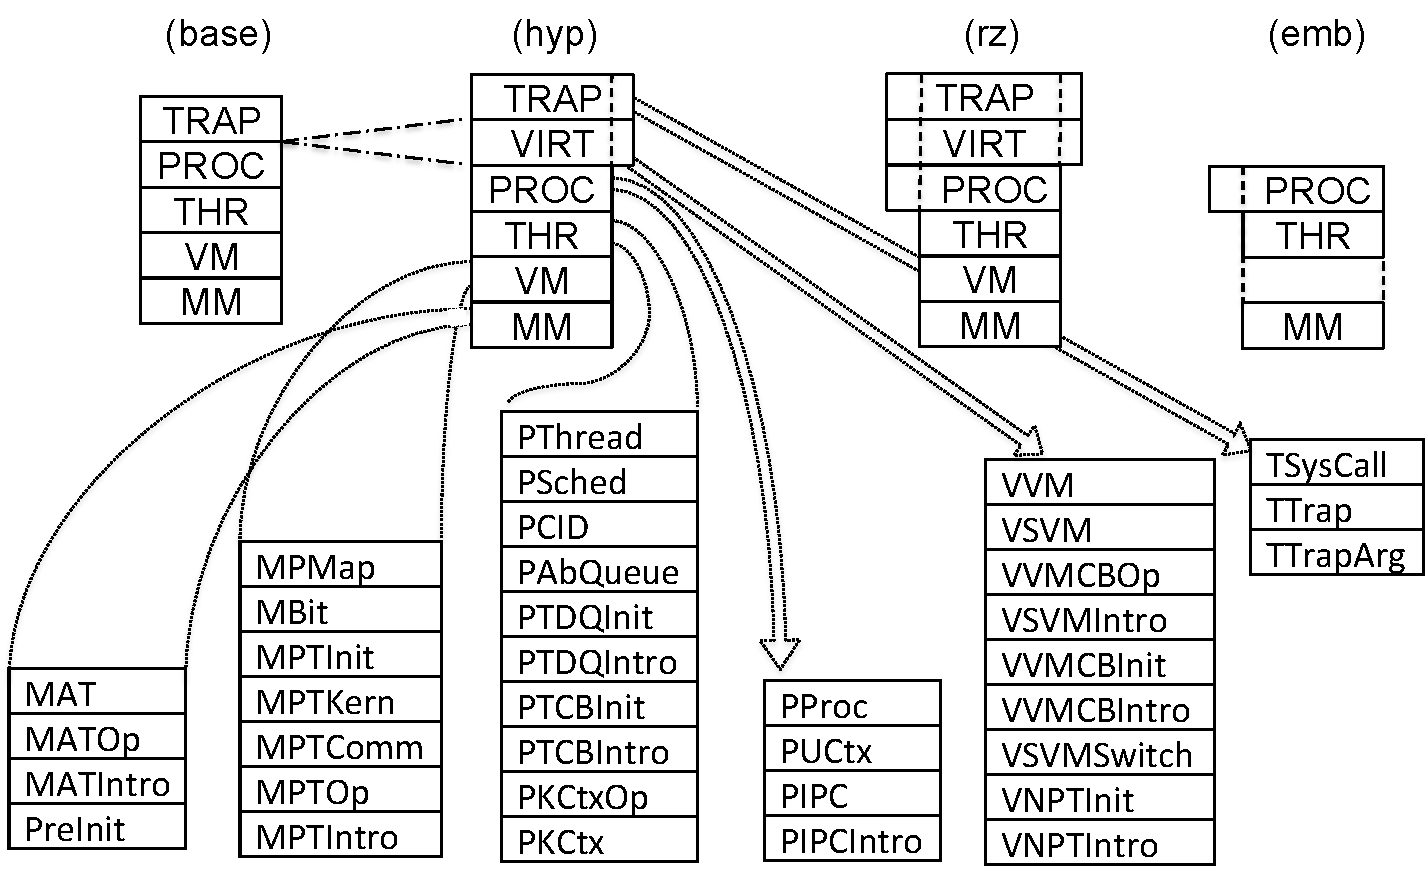
\includegraphics[scale=0.3]{figs/layers}
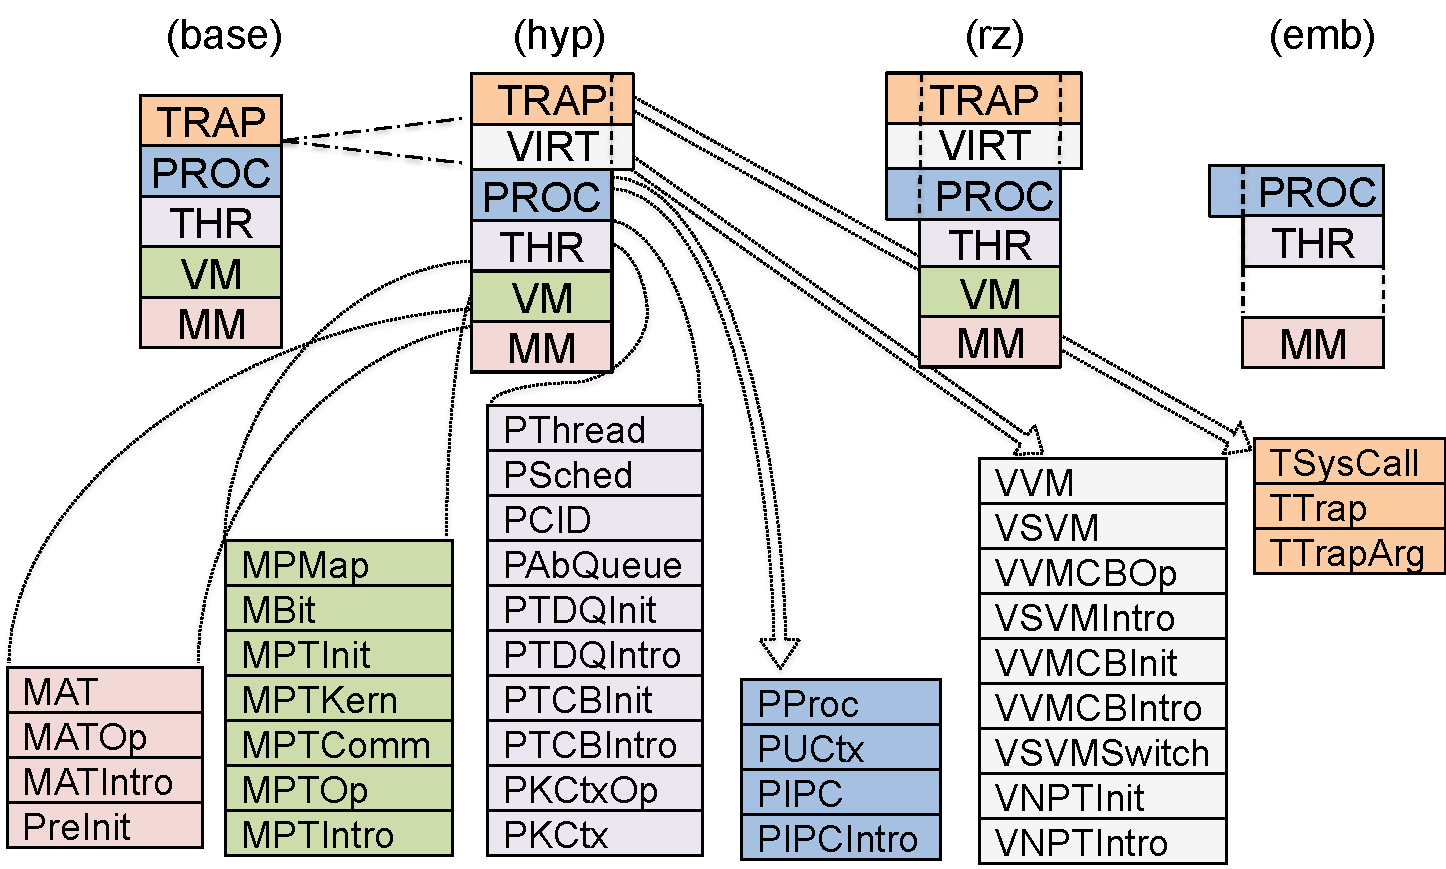
\includegraphics[scale=0.31]{figs/layers2} 
\caption{Various \mCTOS{} layer structures.
Layer short-hands: TRAP: interrupt handling; VIRT: virtualization;
PROC: process management; THR: thread management;
VM: virtual memory; MM: physical memory management.}
\label{fig:kernel-layers}
\end{figure}

Finally, kernel initialization is another difficult task
that has been missing from other kernel verification projects.

Previous efforts on certifying initialization have led to massive duplication
of logical components as shown in \cite{vaynberg12}.

The key observation that frees us from such burden is that the traditional
kernel initialization process is not compatible with
\emph{``specify full behavior and hide all underlying details.''}
For example, \textsf{start\_kernel} in Linux
kernel \footnote{\url{https://github.com/torvalds/linux/blob/master/init/main.c\#L501}}
makes a sequence of calls to module initializations.  \mCTOSbase's
initialization (see its call graph in
Fig.\ \ref{fig:mcertikos-init-call-graph}) is a \emph{chain} of calls
to layer initializations; this pattern complies with the guideline that 
initializing one layer should
hide the detail about initializing the lower layers.
%and makes certification possible without extra constructs.
Without layering, the specifications of \emph{all} functions will be populated
with initialization flags for each module they depend on. This
makes encapsulation harder and could also lead to
a quadratic blowup in size and proving effort.

\begin{figure}
%\vspace*{-2pt}
\center
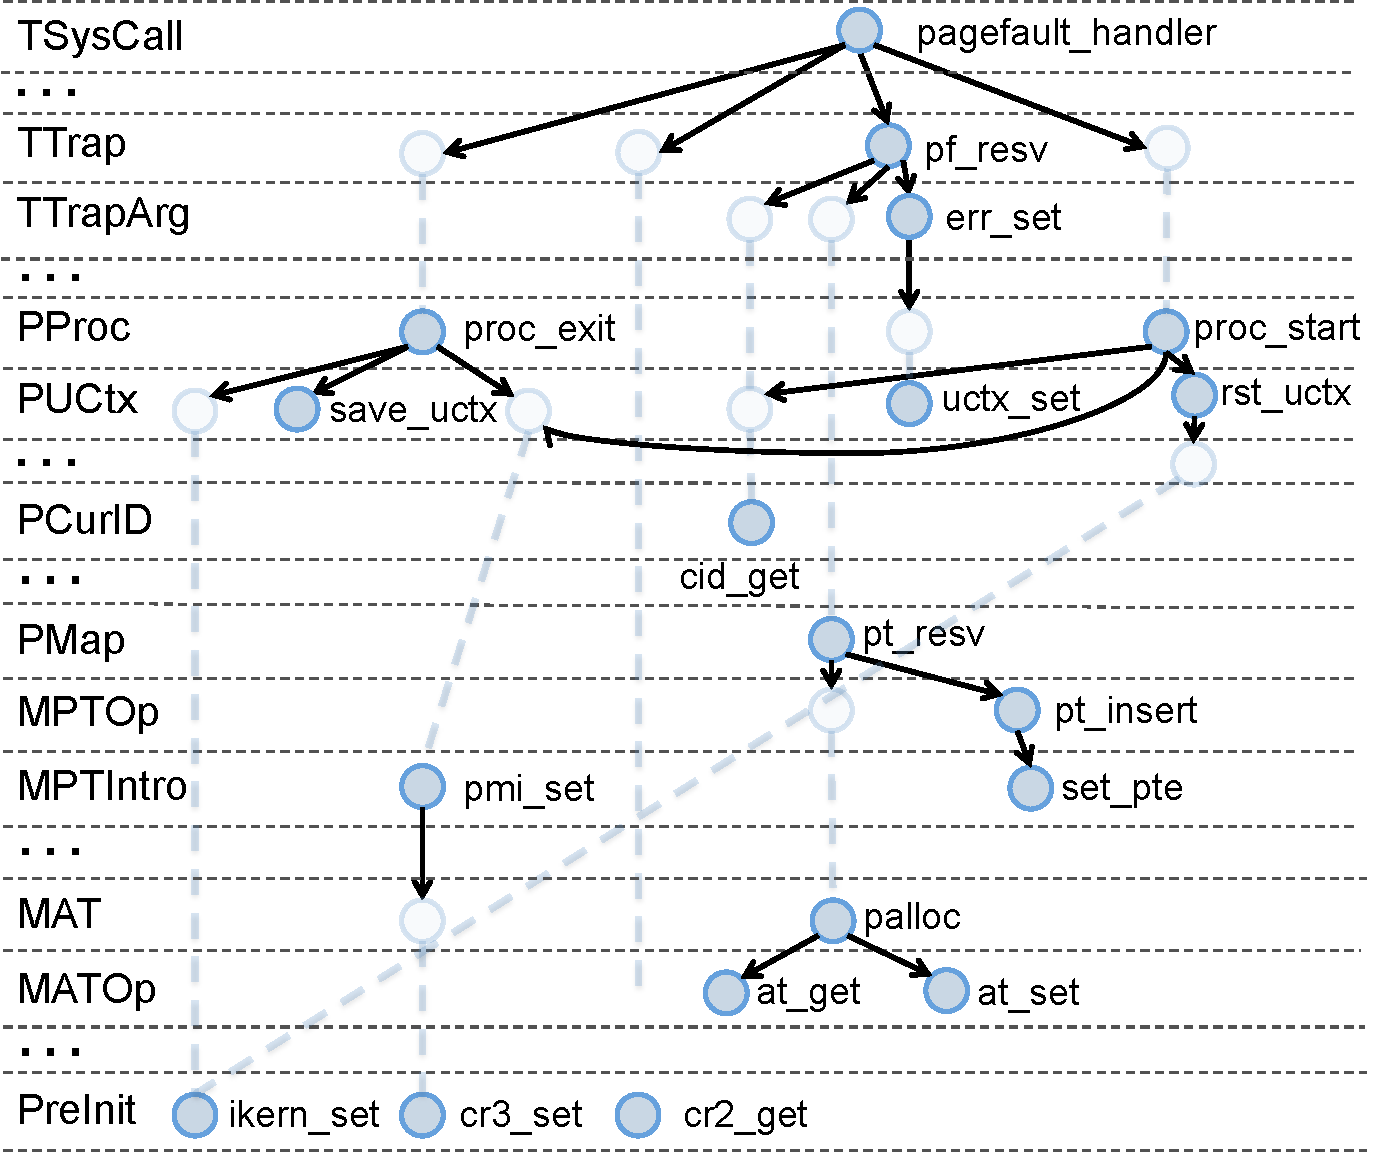
\includegraphics[scale=0.3]{figs/pagefault2}
\caption{Call graph of the page fault handler}
\label{fig:pagefault-call-graph}
\end{figure}

\begin{figure}
\center
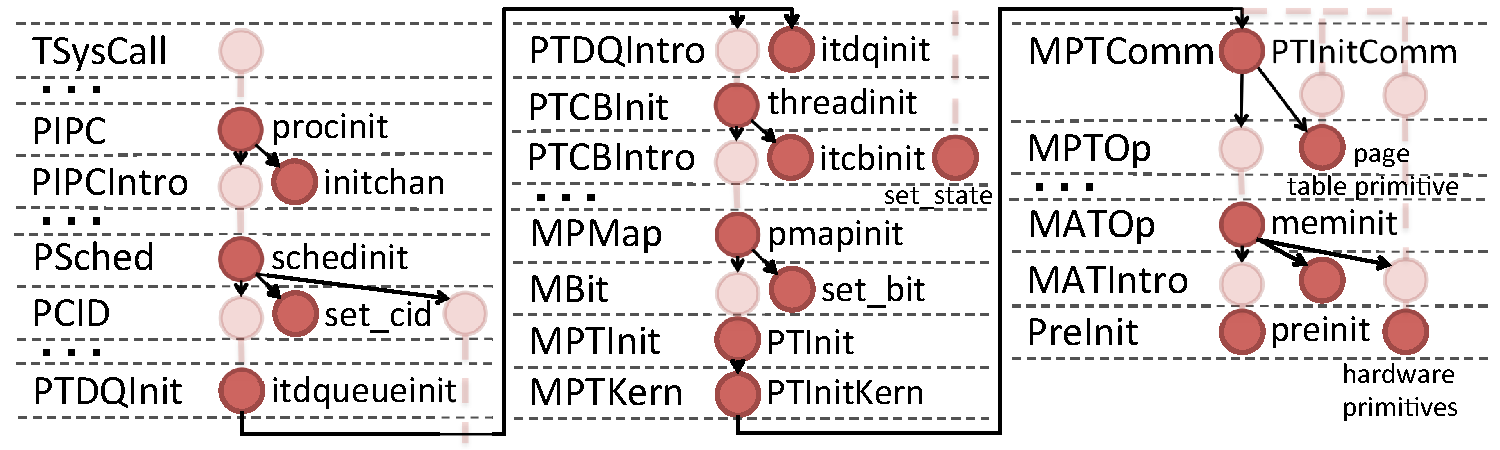
\includegraphics[scale=0.3]{figs/initialization}
\caption{Call graph of \mCTOSbase{} initializer}
\label{fig:mcertikos-init-call-graph}
\end{figure}

%\vspace*{-8pt}
\paragraph{\mCTOShyper{}}
The \mCTOShyper{} kernel provides core primitives to build
full-fledged user-level hypervisors by supporting one of the two
popular hardware virtualization technologies -- AMD SVM.  The primitives
include the operations for manipulating the virtual machine status,
handling VMEXITs, starting or stopping a virtual machine, {\it etc}.
The details of virtualization, e.g., the virtual machine control block
and the nested page table, are hidden from the guest applications.
The hypervisor functionalities are implemented in nine layers and then
inserted in between process management and interrupt handling layers.
The layered approach allows us to do so while (1) only modeling
virtualization-specific structures when needed; (2) retaining
primitives in the layer interface \textsf{PProc} by systematic lifting; and
(3) adding new primitives (including a new initialization function)
guaranteed not to interfere with existing primitives.

%\vspace*{-8pt}
\paragraph{\mCTOSringz{}}
The \mCTOSringz{} kernel explores a different dimension---instead
of adding intermediate layers, we augmented a few existing layers 
(in \mCTOShyper{}) with support of ring 0 processes.
The main modification is at
\textsf{PProc}, where an additional kind of threads is defined.
However, all the layers between \textsf{PProc} and \textsf{TSysCall} also
need to be extended to expose the functionality as system calls.
Thankfully, since all the new primitives are already described in deep
specifications, lifting them to system calls only requires equality
reasoning in Coq.

%\vspace*{-8pt}
\paragraph{\mCTOSembed{}}
The \mCTOSembed{} kernel cuts features down to a bare minimum: it does
not switch to user mode, hence does not require memory protection and
does not provide system call interfaces.  This requires \emph{removing}
features instead of adding them.  Since the layered structure minimizes
entanglements by eliminating unnecessary dependencies and code coupling,
the removal process was relatively easy and straightforward.
Moreover, removing the top 12 layers requires no additional
specifications for those now top-level primitives---deep specifications
are suitable for both internal reasonings and external descriptions.  Thread and process
management layers now sit directly on top of physical memory
management; virtual memory is never enabled.  The
layers remain largely the same barring the removal of primitives
mentioning page tables.

\section{Verifying the \mCTOSbase{} Kernel}
\label{sec:seq:base}

\begin{comment}
\begin{figure*}
\begin{center}
\begin{scriptsize}
\begin{tabular}{ |l|l||l|p{4.5cm}| }
  \hline
  \multicolumn{2}{|c||}{\textbf{Memory Management}} 
  & \multicolumn{2}{|c|}{\textbf{Thread and Process Management}} \\
  \hline
  \hline    
  \multicolumn{2}{|l||}{\textbf{abstract state}} 
  & \multicolumn{2}{|l|}{\textbf{abstract state}}\\
  \hline
  \verb"AT" & physical page allocation table
  & \verb"kctxp" & kernel context (\verb"kctx") pool\\
  \hline 
  \verb"PFInfo" & save the address and \verb"PC" that page fault occurs
  & \verb"Ltdqp" & low abstract thread queue pool\\
  \hline
  \verb"ptp" & page table (\verb"pt") pool 
  
  & \verb"Htdqp"& high abstract thread queue (\verb"Htdq") pool\\ 
  \hline
   \verb"ipt"& whether \verb"pt"'s invariant  should hold or not
  
  & \verb"uctxp" & user context pool\\
  \hline
\verb"PT" & index of the current \verb"pt"
  & \verb"chanp" & channel pool\\
  \hline
  \verb"pbit" & bit map for free \verb"pt" indexes
  & \verb"Htcbp"& high abstract TCB pool \\
  \hline
  \multicolumn{2}{|l||}{\textbf{primitive}} 
  & \multicolumn{2}{|l|}{\textbf{primitive}}\\
  \hline	
  \verb"setcr3" & set the starting address of the \verb"pt"
  & \verb"kctx_new" & allocate the first free \verb"pt" and \verb"kctx"\\
  \hline
  \verb"meminit" & initialize the allocation table
  & \verb"Henqueue" & append a thread to the \verb"Htdq"\\
  \hline
  \verb"palloc" & allocate a page 
  & \verb"thread_kill" & kill and free a thread\\
  \hline
  \verb"pt_insrt" & insert a page map into a given \verb"pt" 
  & \verb"thread_sleep" & sleep, schedule to the 1st ready thread\\
  \hline
  \verb"pt_resv" & allocate a page for a given linear addr 
  & \verb"kctx_switch" & switch \verb"kctx" between threads\\
  \hline 
  \verb"PTInit" & init kernel's \verb"pt" and enable paging 
  & \multirow{2}{*}{\texttt{resv\_chan}} & 
  receive msg from the channel, wake\\
  \cline{1-2}
  \verb"pt_new" & allocate the first free \verb"pt" & & up the first sleeping thread
    \\	  
  \hline
  \hline
  \multicolumn{2}{|c||}{\textbf{Virtualization}}
  &\multicolumn{2}{|c|}{\textbf{Trap Handler}} \\
  \hline
  \hline    
  \multicolumn{2}{|l||}{\textbf{abstract state}} 
  & \multicolumn{2}{|l|}{\textbf{primitive}} \\
  \hline
  \verb"npt" & nested page table for guest
  & \verb"trap_arg" & get arguments of system calls\\
  \hline
  \verb"hctx"& host context
  & \verb"hpagefault" & page fault handler\\ 
  \hline
  \verb"vmcb" & virtual machine (\verb"VM") control control block
  & \verb"sys_yield" & system calls for yielding\\
  \hline
  \verb"xvmst" & registers not saved in \verb"vmcb" 
  & \verb"sys_wait_chan" & system calls to sleep on a channel\\
  \hline
  \multicolumn{2}{|l||}{\textbf{primitive}} 
  & \verb"sys_run_vm" & system calls to run \verb"VM"\\
  \hline	
  \verb"npt_insrt" & insert into the nested page table
  & \verb"sys_proc_create" & system calls to create a process\\
  \hline
  \verb"switch2guest" &  switch to guest mode 
  & \verb"sys_getexitinfo" 
  & get the information about \verb"VM" exit\\
  \hline
  \verb"set_vmcb" & set value in virtual machine control block
  & \verb"sys_injectevent" & inject interrupt and exception to \verb"VM"\\
  \hline 
  \verb"run_vm" & save host context, restore \verb"vmcb", start \verb"VM" 
  & \verb"kernel_init" & initialization function of the kernel\\  
  \hline  

\end{tabular}
\end{scriptsize}
\caption{Key abstract states and primitives for \mCTOSbase{} and \mCTOShyper{}}
\label{table:layers}
\end{center}
\vspace*{-14pt}
\end{figure*}
\end{comment}

The \mCTOSbase{} kernel is divided into six main parts.  From the
bottom layer which corresponds to the physical machine to the top
layer providing system calls, those are the pre-initialization module
(1 layer, Section~\ref{sec:base:preinit},
Figure~\ref{fig:base:pmm:layers}), physical memory management (3 layers,
Section~\ref{sec:base:pmm}, Figure~\ref{fig:base:pmm:layers}), virtual
memory management (7 layers, Section~\ref{sec:base:vmm},
Figure~\ref{fig:base:vmm:layers}), thread management (10 layers,
Section~\ref{sec:base:tm}, Figure~\ref{fig:base:tm:layers}), process
management (4 layers, Section~\ref{sec:base:pm},
Figure~\ref{fig:base:pm:layers}), and the trap handler (3 layers,
Section~\ref{sec:base:trap}, Figure~\ref{fig:base:trap:layers}).  In
this section, we go through each module by describing its
layers from bottom to top.  

\paragraph{How to read figures describing modules}
In each figure describing a module, each rounded corner box is a layer
with the name in bold. Underneath the name is the list of abstract
states separated by commas. Primitives are enclosed in boxes
touching the bottom edge of the layer; green filling indicates
initialization primitives. Boxes filled with purple represent
a collection of primitives.

Lines with a dot on one end mark refinement relations: the box on the
flat end refines the primitive on the dotted end. On the flat end, the
box can be either a primitive, in the case of \emph{pass-through}
primitives which are implemented in layers further down in the stack,
or a function implementation (an actual piece of code) represented by
a small blue box touching the top of the layer in which it is
implemented.  A function may have outgoing arrows point to primitives
it calls as illustrated in Figure\ \ref{fig:refine}c; those without
outgoing arrows correspond to Figure\ \ref{fig:refine}b.
\ronghui{Fix}

\subsection{Pre-initialization}
\label{sec:base:preinit}
The pre-initialization module only contains the bottom-most layer
\code{PreInit}, which is shown at the bottom of Figure~\ref{fig:base:pmm:layers} outside the red dashed box. It is used to model the x86 hardware and axiomatizes the
hardware behaviors that are necessary to obtain end-to-end behaviors
across the kernel and the user space. These behaviors include page
table walk upon memory load when paging is turned on, saving and
restoring part of the trap frame in the case of interrupts, and switching
the stack in the case of ring switch.

The \code{x86} object is the only layer object in the \code{PreInit} layer.
It extends the CompCert assembly semantics
to model the low-level features of the machine.
Its abstract state consists of control registers,
a physical memory map \code{MM},
and a kernel mode flag \code{ikern}.
Its primitives consist of
getter-setter functions for control registers and \code{MM},
and a function models the transition between user and kernel mode.

The state component \code{MM} is the abstraction of the
E820 memory map provided by the bootloader.
The control registers \code{CR0}, \code{CR2}, and \code{CR3},
are used to model the behavior
of the processor's memory management unit (MMU),
which is specified by the \emph{memory accessors}
of \code{PreInit}.
When paging is enabled (as indicated by \code{CR0}),
memory accesses (\ie, load and store) made by both the kernel and the user programs
are translated using the page map pointed to by \code{CR3}
(shown in Figure~\ref{fig:seq:mem1}).
When a page fault occurs,
the corresponding information is stored in \code{CR2}
and the page fault handler is invoked.

\begin{figure*}[t]\centering
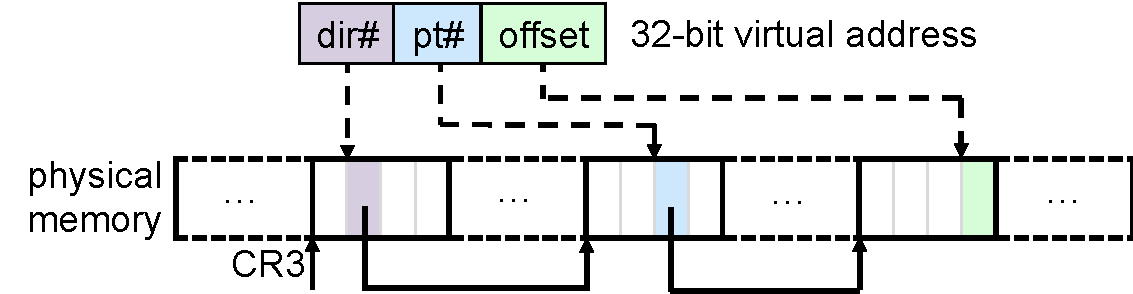
\includegraphics[scale=.55]{figs/mem_model_1} 
\caption{Address translation at \code{PreInit} layer}
\label{fig:seq:mem1}
\hrulefill
\end{figure*}

The logical flag \code{ikern} indicates
whether the processor is currently in kernel or user mode.
The \code{kernel\_mode} predicate of \code{PreInit}
is defined as $``\code{ikern} =\code{true}"$.
Some privileged
memory regions (\eg, allocation table) and 
instructions (\eg, modifying control registers)
are only available in kernel mode.
\ignore{
The switch function models the change of the \code{ikern} flag
and the remaining tasks involved with trap handling,
such as saving and restoring user and kernel contexts,
and dispatch over the trap type,
are verified at the assembly level.
}

The initialization primitive at this bottom-most layer is the bootloader,
which initializes \code{MM} and necessary drivers
(\eg, timer, keyboard, serial, {\it etc.}),
loads the kernel into the memory,
and sets the initialization flag $\code{init}$ to be \code{true}.


\subsection{Physical memory management}
\label{sec:base:pmm} 

{
\begin{figure}\centering
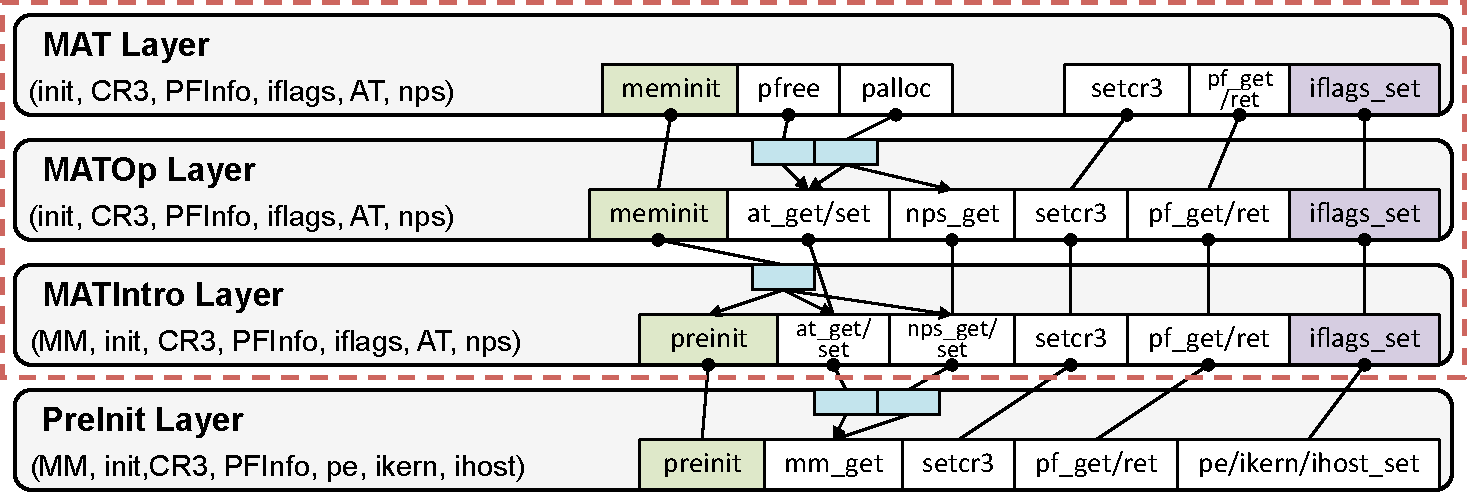
\includegraphics[scale=0.5]{figs/pmm_layer}	
\caption{Layers of physical memory management}
\label{fig:base:pmm:layers}
\hrulefill
\end{figure}
}

Based on the pre-initialization layer and its memory
accessors,
the physical memory management abstracts the physical page allocation table
into \code{page} objects.
To better reason about access control and isolation in the case of
the dynamic resource allocation, each physical page
object maintains a \emph{logical} state containing ownership information,
and the page is only allowed to be accessed by its owners.

The physical memory management of \mCTOSbase{}
consists of  3 layers, which are shown in the red dashed box in
Figure~\ref{fig:base:pmm:layers}.
\ignore{
The module first
defines a getter-setter layer \verb"MATIntro", followed by an
abs-kernel-fun layer \verb"MATOp" where a new initializer is defined,
and then another abs-kernel-fun layer \verb"MAT" which provides the
physical page allocator.
}
The module introduces two new abstract states: \verb"nps", the number
of physical pages, as well as \verb"AT", the page allocation table
indicating whether a memory page is free or not.  The states \verb"AT"
and \verb"nps" are initialized using in \verb"meminit" using the information
in \verb"MM". The module also exports two primitives
\verb"palloc" and \verb"pfree", allocating and freeing memory pages,
respectively.

\paragraph{Enforcing memory quotas}

Another function of the physical memory management is to dynamically
track and bound the memory usage (in terms of number of dynamically-allocated
pages) of processes based on their id.

In \mCTOSbase{}, we consider every unique
integer (up to some predefined maximum, currently $2^{18}$) to represent
a different agent or principal. We refer to this integer as the agent's
id, and we use it for all layer objects owned by that agent. % For example,
% whenever \mCTOSbase{} receives a request to spawn a process, it picks some 
% currently unused id $i$ and creates a new container, page map, and thread 
% control block, all of which are bound to the same id $i$. Thus
% The id serves
% as a simple and global way to relate various kernel objects to a single agent.


The MContainer layer introduces a notion of container, inspired by container 
objects in the HiStar operating system~\cite{zeldovich06}. 
Whenever a new agent (id) is created in \mCTOSbase{}, a container is created for the agent 
that dynamically keeps track of its memory usage. 
An agent's usage may increase for a few reasons, including a direct request for 
dynamically-allocated resources, or a successfully-handled page fault. Each container 
object is initialized with some maximum \emph{quota}; any attempt for an agent to increase 
its usage beyond this quota will be denied by the kernel. Furthermore, the kernel maintains a mapping of ids to containers using
a hierarchical tree structure. Whenever an agent's process makes a request to spawn a
new process, the new container is added as a child to the requesting agent's container,
and the new container's quota is taken from the requester's.

With this notion of container, we are able to prove a theorem about reliability of 
dynamic memory allocation: agents' requests for additional resources will always be 
fulfilled as long as their quota is not exceeded.
Furthermore, from the viewpoint of information-flow security, resource quotas close the 
potential for two different processes to communicate via allocation requests.
Hence quota enforcement provides an additional level of security for \mCTOSbase{}.
%
We plan to extend the concept of containers to other types of
resources in the future. For example, we could maintain a time-slice quota
for each agent.  This would provide a foundation for reasoning about
liveness properties for processes and security breaches via timing
channels.


\ignore{
To verify the implementations of \verb"palloc" and \verb"pfree",
we prove the following invariant at layer \verb"MATOp".
\begin{invariant}
\label{inv:atable}
After the initialization (\verb"init" = \verb"true"),
(1) $2^{18} \le \verb"nps" < 2^{20}$, (2) physical page in low memory part has type \verb"PG_KERNEL", and
(3) physical page in high memory part has type \verb"PG_KERNEL" or \verb"PG_NORMAL".
\end{invariant}

\begin{figure}[ht]\scriptsize
$$
\begin{array}{l|l}
\begin{array}{l}
\verb"typedef enum {"\\
\verb"  PG_RESERVED,"\\
\verb"  PG_KERNEL,"\\
\verb"  PG_NORMAL"\\
\verb"} pg_type;"\\
\\
\verb"struct pginfo {"\\
\verb"  pg_type	t;"\\
\verb"  int	used;"\\
\verb"};"\\
\\
\verb"struct pginfo AT[1<<20];"
\end{array}
&
\begin{array}{l}
\verb+Inductive pg_type :=+\\
\verb+| PG_RESERVED+\\  
\verb+| PG_KERNEL+\\  
\verb+| PG_NORMAL.+\\
\\
\verb+Inductive pginfo :=+\\
\verb+| ATValid (t: pg_type)+\\
\verb+          (used: bool)+\\ 
\verb+| ATUndef.+\\
\\
\verb+Definition AT :=+\\
\verb+      ZMap.t pginfo.+\\
\end{array}
\\\vspace*{-14pt}
\end{array}
$$ 
\caption{Concrete vs. abstract page allocation table}
\label{fig:abs:atable}
\vspace*{-14pt}
\end{figure}

}


\subsection{Virtual memory management}
\label{sec:base:vmm} 

\begin{figure}\centering
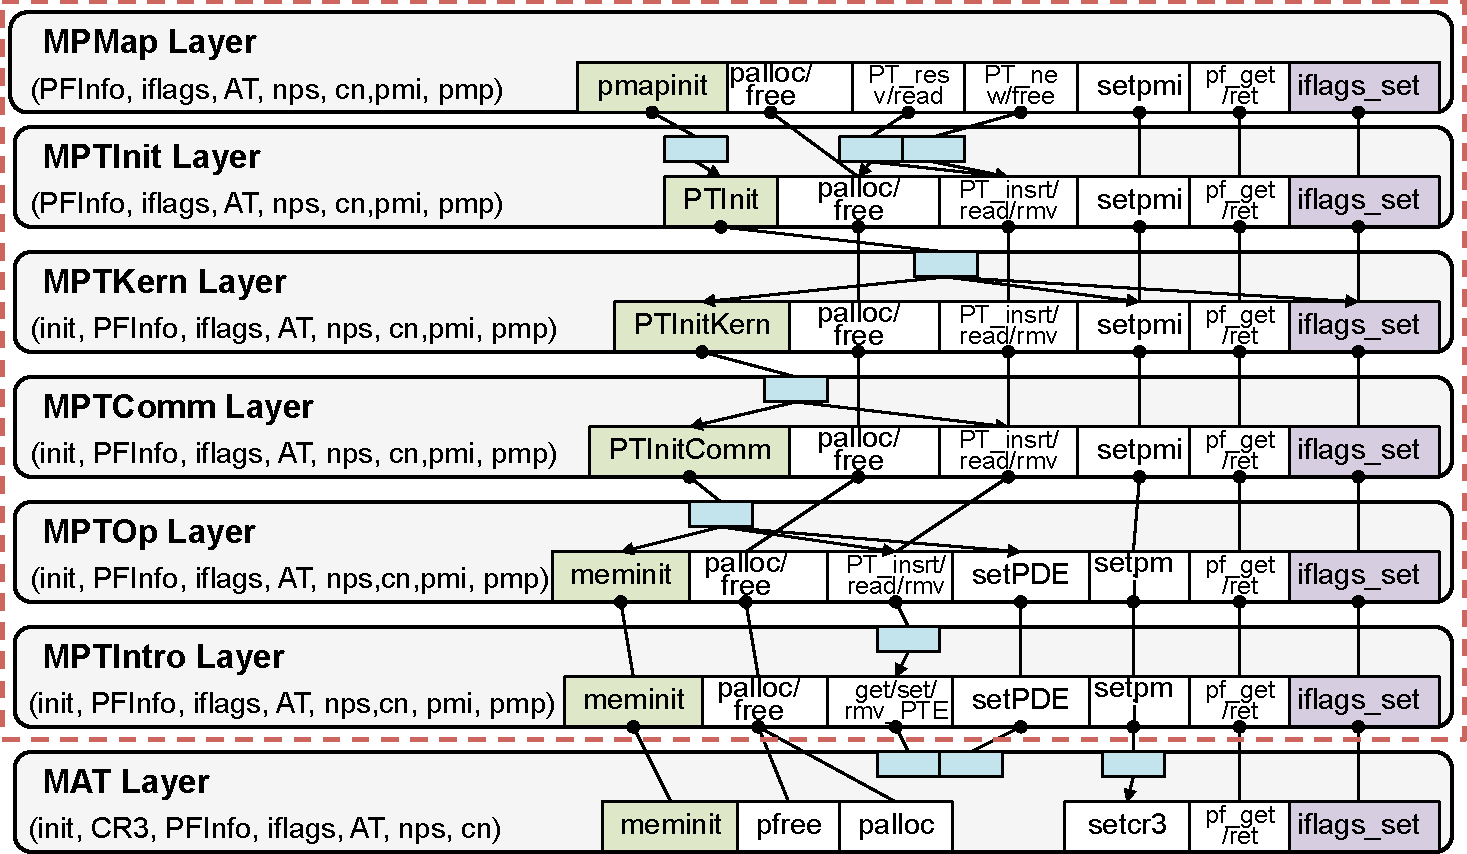
\includegraphics[scale=0.5]{figs/vmm_layer}	
\caption{Layers of virtual memory management}
\label{fig:base:vmm:layers}
\hrulefill
\end{figure}

\ignore{
We still focus on memory in the next module, however, we turn our
attention to user programs' needs.  
}
On top of physical memory management,
the virtual memory management provides consecutive virtual address spaces.
As shown in
Figure~\ref{fig:base:vmm:layers}, the virtual memory management of
\mCTOSbase{} consists of 7 layers: getter-setter layer \verb"MPTIntro"
defines two new abstract states, the page map pool \verb"pmp" (which
consists of 64 page tables) and the page map index \verb"pmi" (which
points the current page table); abs-kernel-fun layer \verb"MPTOp"
introduces primitives on page maps including \verb"pt_insrt" and
\verb"pt_read"; the following three abs-kernel-fun layers
\verb"MPTComm", \verb"MPTKern", and \verb"MPTInit" build up the
initialization function \verb"PTInit"; getter-setter layer \verb"MBit"
creates bitmap for page map availability; and, finally,
abs-kernel-fun layer \verb"MPMap" wraps up page map allocation and
release.

Starting from the \verb"MPTIntro" layer, we 
introduce a new memory accessors.
As shown in Figure~\ref{fig:seq:mem2},
the
address translation at this layer is defined
using \verb"pmp" and \verb"pmi" instead of the physical two-level page
table and the \verb"CR3" register.  The contextual refinement relation
between these two kinds of address translations guarantees that the
value in the \verb"CR3" register is always a valid starting address of
a well-formed page table.

\begin{figure*}[t]\centering
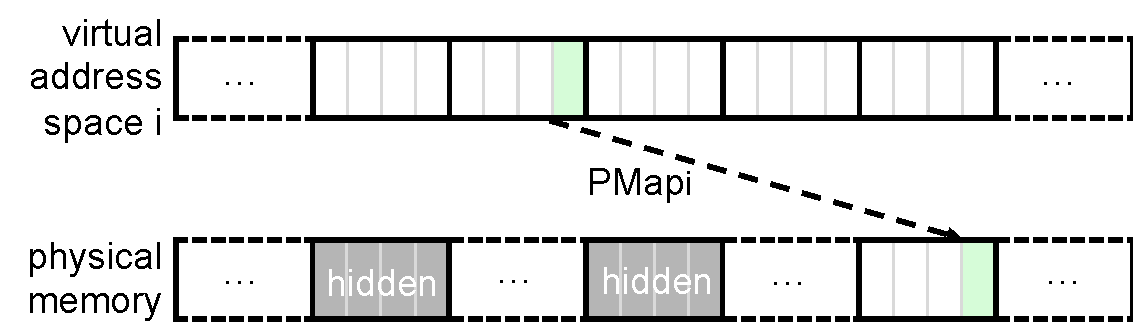
\includegraphics[scale=.55]{figs/mem_model_2} 
\caption{Address translation at \code{MPTInit} layer}
\label{fig:seq:mem2}
\hrulefill
\end{figure*}

We proved not only that the primitives of virtual memory management
manipulate the address space correctly,
but also that the initialization procedure sets up the two-level page maps properly
in terms of hardware address translation.
After paging is enabled, both kernel modules and user processes
run in a virtual address space.
To ensure the correctness of these kernel modules and user processes on top of virtual memory
management, we prove the following invariants :
\begin{invariant}
\label{inv:seq:virtual}
1) paging is enabled only after the initialization of virtual memory management;
2) the memory regions that store kernel-specific data must have the kernel-only 
permission in all page maps;
3) the page map used by the kernel is an identity map
4) the non-shared parts of user processes' memory are isolated.
\end{invariant}

Invariant~\ref{inv:seq:virtual} no longer holds 
if the privileged primitive that sets the \code{CR3}
register is present in the layer, as the unknown context code may write
an invalid address into \code{CR3} using the provided primitive. To solve this issue, 
$\code{MPTIntro}$
layer is introduced with a wrapper function 
$\code{setpmi}$
that takes the process $id$ as argument,
instead of an actual address. Then the function sets \code{CR3} to the
starting address of the predefined corresponding process's page table structure.
The primitive $\code{setcr3}$ that directly sets the \code{CR3} register is hidden from the
new layer, and the invariants are introduced in this layer.
This is one of the rare cases where performance overhead is introduced
(one extra function call due to the wrapper).
It is possible to use CompCertX's function-inlining optimization
to remove this overhead (this is left as future work).
\ronghui{Fix me}

\paragraph{The shared memory management} provides a protocol to share physical
pages among different user processes. 
It provides an infrastructure to map a physical page into multiple
processes' page maps in different address spaces.
Our ownership mechanism ensures that the page can only be freed once 
all processes release ownership.

\ignore{
\begin{figure}[ht]\scriptsize
$$
\begin{array}{l|l}
\begin{array}{l}
\verb"#define PDES    1024"\\	
\verb"#define PTES    1024"\\
\verb"#define PTEP    0x001"\\
\verb"#define PTEW    0x002"\\
\verb"#define PTEU    0x004"\\
\\
\verb"struct pmap {"\\
\verb"  uint32_t pd[PDES];"\\
\verb"  uint32_t pt[PDES][PTES];"\\
\verb"};"\\
\\
\verb"struct pmap pmp[64];"
\end{array}
&
\begin{array}{l}
\verb+Inductive PTPerm :=+\\
\verb+| PTEP | PTEW | PTEU.+\\
\verb+Inductive PTE:=+\\
\verb+| PTEV (v: block)+\\
\verb+       (p: PTPerm)+\\
\verb+| PTEUnPresent+\\
\verb+| PTEUndef.+\\
\verb+Definition PT :=+\\
\verb+      ZMap.t PTE.+\\
\verb+Inductive PDE :=+\\
\verb+| PDEV (pt: PT)+\\
\verb+| PDEUndef.+\\
\verb+Definition pmap :=+\\
\verb+      ZMap.t PDE.+\\
\verb+Definition pmp :=+\\
\verb+      ZMap.t pmap.+
\end{array}
\\\vspace*{-14pt}
\end{array}
$$ 
\caption{Concrete vs. abstract page table}
\label{fig:abs:ptable}
\end{figure}

Since \verb"PTInit"  enables paging after initializing \verb"pmp", the addressing mode changes inside the function execution. Therefore, verification of the initialization function need to enforce that:
\begin{invariant}
\label{inv:pagemap}
When paging is enabled (\verb"pe" = \verb"true"),
(1) the low memory part of all page maps in \verb"pmp" must be identity maps, and
(2) if in the kernel mode (\verb"kern" = \verb"true"), the current page table (\verb"pmp[pmi]") must be an identity map.
\end{invariant}
}


\subsection{Thread management}
\label{sec:base:tm} 

{
\begin{figure}\centering
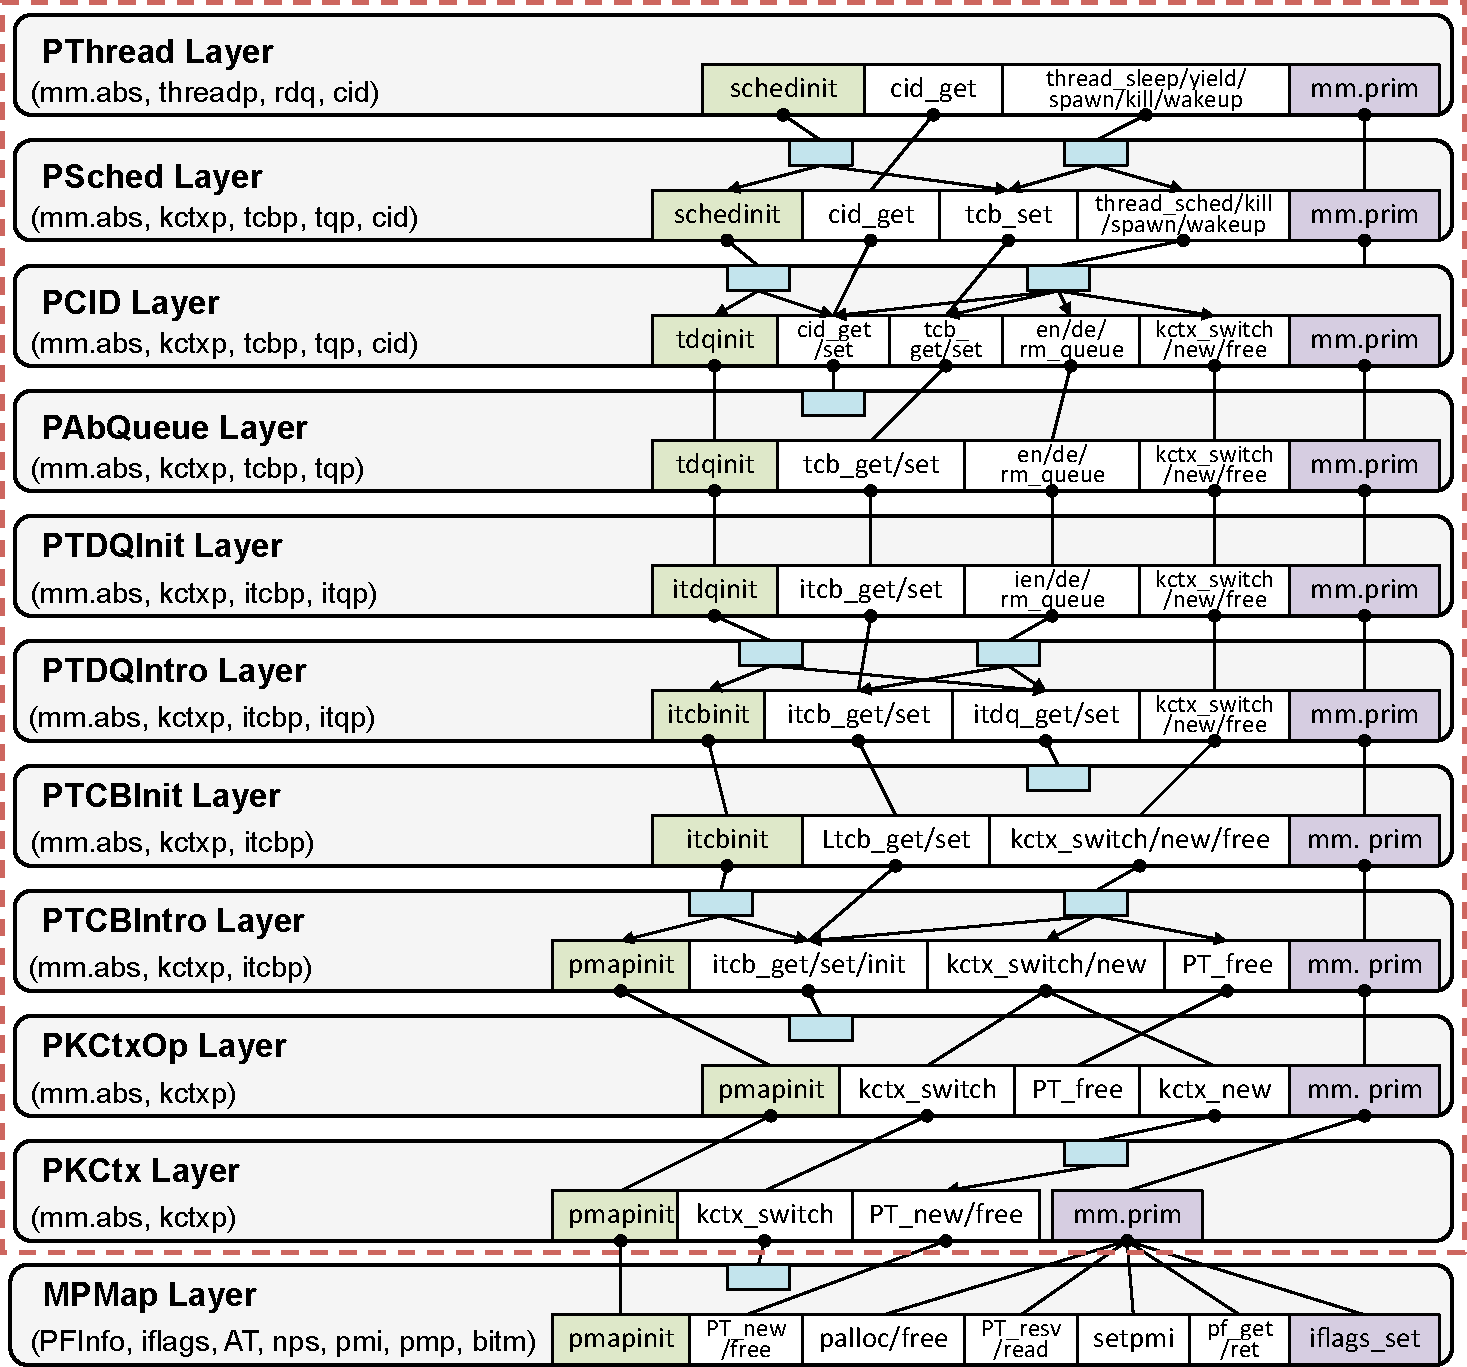
\includegraphics[scale=0.5]{figs/tm_layer}	
\caption{Layers of thread management}
\label{fig:base:tm:layers}
\hrulefill
\end{figure}
}

\ignore{
\begin{figure}[ht]\scriptsize
$$
\begin{array}{l|l}
\begin{array}{l}
\verb+Record thread := {+\\
\verb+  id: Z;+\\ 
\verb+  kernel_context: kctx;+\\
\verb+  TCB: tcb;+\\
\verb+  sleep_queue: tdq+\\
\verb+}+
\end{array}
&
\begin{array}{l}
\verb+Record process := {+\\
\verb+  td: thread;+\\
\verb+  pagemap: pmap;+\\
\verb+  user_context: uctx;+\\
\verb+  channel: chan+\\
\verb+}+
\end{array}
\\\vspace*{-14pt}
\end{array}
$$ 
\caption{Abstract thread and process}
\label{fig:abs:threadproc}
\end{figure}
}


The thread management module consists of 10 layers and is
shown in Figure~\ref{fig:base:tm:layers}.  The layers \verb"PKCtx",
\verb"PTCBIntro", and \verb"PTDQIntro" are getter-setter layers
defining the kernel context pool \verb"kctxp", the intermediate
abstract thread control block (TCB) pool \verb"itcbp", and the
intermediate thread queue pool \verb"itdqp", respectively, while
\verb"PKCtxOp", \verb"PTCBInit", and \verb"PTDQInit" are
abs-kernel-fun layers introducing operations over these abstract
states. The top four layers then finalize the abstraction into the
thread pool \verb"threadp", the ready queue \verb"rdq", and the
current thread id \verb"cid", and provide the standard thread
primitives such as \verb"thread_spawn" and \verb"thread_yield".
\ignore{
{
\setlength{\floatsep}{-10pt}
\setlength{\belowcaptionskip}{-10pt}
\vspace*{-10pt}
\begin{figure}[ht]\tiny
$$
\begin{array}{l|l}
\begin{array}{l}
\verb+struct tcb *+\\
\verb+dequeue(struct tdq * queue){+\\
\verb+  struct tcb * head, next;+\\
\verb+  struct tcb * pid = null;+\\
\verb+  if(queue == null)+\\
\verb+    return pid;+\\
\verb+  else {+\\
\verb+    head = queue -> head;+\\
\verb+    if (head == null)+\\
\verb+      return pid;+\\
\verb+    else {+\\
\verb+      pid = head;+\\
\verb+      next = head -> next;+\\
\verb+      if(next == null) {+\\
\verb+        queue -> head = null;+\\
\verb+        queue -> tail = null;+\\
\verb+      } else {+\\
\verb+        next -> prev = null;+\\
\verb+        queue -> head = next;+\\
\verb+      }+\\
\verb+    }+\\
\verb+  }+\\
\verb+  return pid;+\\
\verb+}+
\end{array}
&
\begin{array}{l}
\verb+Function dequeue (d:abs) (i:Z) :=+\\
\verb+match d.itdqp i with+\\
\verb+|TDQV h t =>+\\
\verb+ if zeq h null then+\\
\verb+  Some (d, null)+\\
\verb+ else+\\
\verb+  match d.itcbp h with+\\
\verb+  |TCBV _ n =>+\\
\verb+   if zeq n null then+\\
\verb+   let tdq':=(TDQV null null) in+\\
\verb+    Some (set_itdq d i tdq', h)+\\
\verb+   else+\\ 
\verb+    match d.itcbp n with+\\
\verb+    |TCBV s' _ n' =>+\\
\verb+    let tdq':=(TDQV n t) in+\\
\verb+    let d':=set_itdq d i tdq' in+\\
\verb+    let tcb':=(TCBV s' null n') in+\\
\verb+      Some (set_itcb d' n tcb', h)+\\
\verb+    |_ => None+\\
\verb+    end+\\
\verb+  |_ => None+\\
\verb+  end+\\
\verb+|_ => None+\\
\verb+end+
\end{array}
\vspace*{-14pt}
\end{array}
$$ 
\caption{Concrete vs. intermediate dequeue primitive}
\label{fig:abs:dequeue}
\end{figure}
}

{
\setlength{\floatsep}{-10pt}
\setlength{\abovecaptionskip}{3pt}
\setlength{\belowcaptionskip}{-10pt}
\begin{figure}[ht]\scriptsize
\begin{verbatim}
    Function dequeue (d:abs) (i:Z) :=
      match d.tdqp i with
        | h :: q => Some (set_tdq d i q, h)
        | nil => None 
      end 
\end{verbatim}
\vspace*{-14pt}
\caption{Abstract dequeue primitive}
\label{fig:abs:Hdequeue}
\end{figure}
}

{
\setlength{\floatsep}{-10pt}
\setlength{\belowcaptionskip}{-5pt}
\begin{figure}[ht]\scriptsize
$$
\begin{array}{l|l}
\begin{array}{l}
\verb+Inductive itcb :=+\\
\verb+| TCBUndef+\\
\verb+| TCBV (tds: td_state)+\\
\verb+       (prev next: Z)+\\
\\
\verb+Definition itcbp:=+\\
\verb+      ZMap.t itcb+
\end{array}
&
\begin{array}{l}
\verb+Inductive itdq :=+\\
\verb+| TDQUndef+\\
\verb+| TDQV (head tail: Z)+\\
\\
\verb+Definition itdqp:=+\\
\verb+      ZMap.t itdq+
\end{array}
\vspace*{-14pt}
\end{array}
$$ 
\caption{Intermediate abstract TCB and thread queue}
\label{fig:abs:ltdq}
\end{figure}
}}

In Figure~\ref{fig:queue}, we
presented the concrete implementations of the thread control blocks
and thread queues (using doubly linked lists) as well as the abstract
view of these data structures using Coq lists.  The abstraction 
makes reasoning easier and is used to describe the behaviors of
functions that operate on these data structures.

As an example, the C implementation of the operation \verb"deQ" is shown
in the left panel of Figure~\ref{fig:queue:a} and the corresponding
abstract specification is shown in Figure~\ref{fig:queue2}.
Unfortunately, the drastic difference between the two renders
the verification extremely complicated.

To the rescue, again, is the layering design.  The fact that the two
layers are too far apart (to be easily verifiable) calls for more
layers in between.  Recall that layered specification and verification
aim at specifying and verifying each implementation at the right
abstraction level.  The Coq list is apparently too high an abstraction
for the doubly linked list and we should find a middle ground between
them.  One major gap between the two is that in a doubly linked list,
a node {\em contains} references to the next and the previous nodes,
while in a Coq list, it is the \verb"cons" cell that holds the link to
the current and the next nodes.

This is why we introduce the intermediate abstract TCB and thread
queue in the bottom 6 layers in this module.  The definitions of the
intermediate data structures 
and the dequeue specifications are shown in
Figure~\ref{fig:queue:b}.
Since we store the previous and next
nodes as numbers in \verb"itcb", we are able to mimic the C code
closely, resulting in a much simpler proof.

Based on these intermediate layers, we then introduce the
\verb"PAbQueue" layer, which contains the TCB and dequeue specifications in
Figure~\ref{fig:queue2}. This layer is then used to define
primitives on threads.  It still takes some effort to prove the
refinement relation but it is more manageable as they are both Coq
functions. 

One interesting aspect of the thread management component is the 
context switch function. 
This assembly function saves the register set
of the current thread and restores the register set from 
the kernel context of another thread.
Since the instruction pointer register (\code{EIP}) and stack pointer register (\code{ESP}) 
are saved and restored in this procedure,
we can show that this function reflects the C-level behavior
and restores the continuation of a thread's execution.
Even though this kernel context switch function is verified at 
assembly level,
we prove that it will not violate the convention of ClightX execution.
This enables us to link it with other code that is verified at C-level
and compiled by CompCertX. 

\ignore{
\begin{invariant}
\label{inv:tdqueue}
(1) Every thread with the state \verb"TD_READY" is in the ready queue;
(2) Every thread with the state \verb"TD_SLEEP" is in one and only one sleeping queue;
(3) All other threads are neither in the ready queue nor in any of the sleeping queues.
\end{invariant}
}

\ignore{
As shown in Fig.~\ref{fig:abs:threadproc} (left), an abstract thread \verb"thread" consists of the thread id, kernel context, TCB and a sleeping queue.
}

\begin{comment}
(In the figure, abstract states and primitives are abbreviated as \verb"mm.abs" and \verb"mm.prim", marked as purple.)
\end{comment}

\subsection{Process management}
\label{sec:base:pm} 


{
\begin{figure}\centering
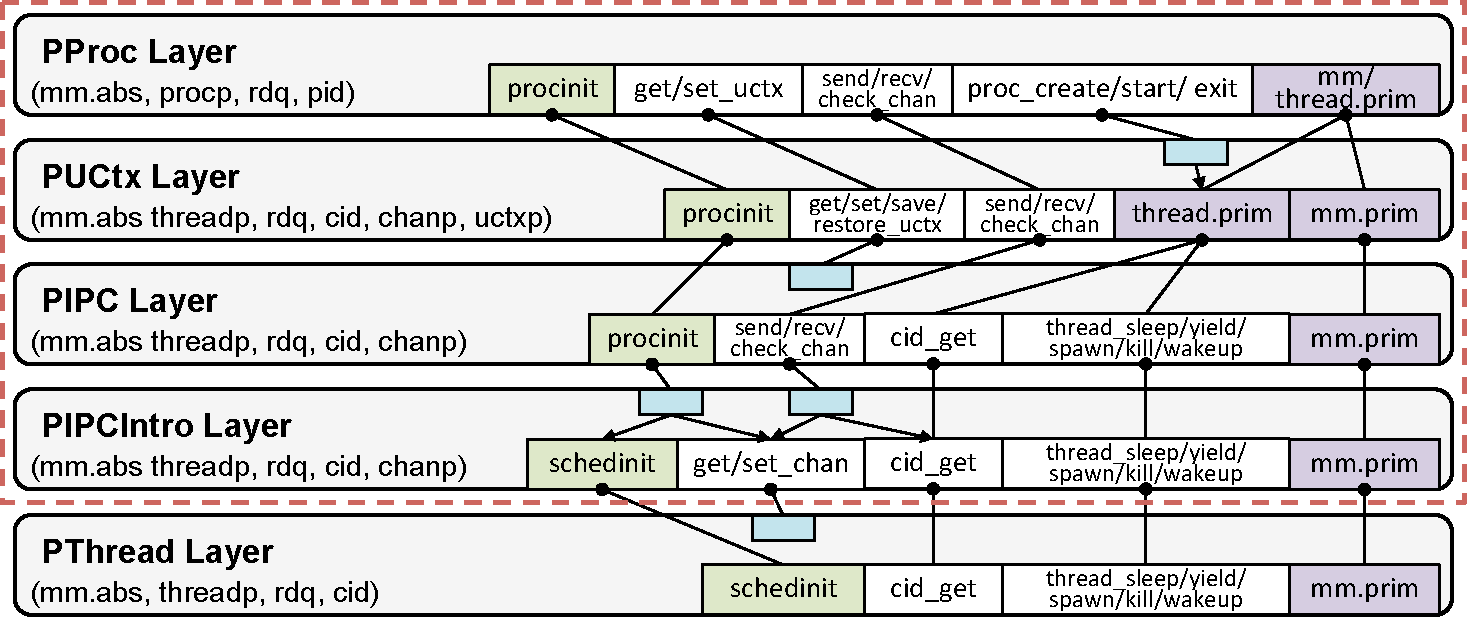
\includegraphics[scale=0.5]{figs/pm_layer}	
\caption{Layers of process management}
\label{fig:base:pm:layers}
\hrulefill
\end{figure}
}
 
Figure~\ref{fig:base:pm:layers} shows the 4 layers of the process
management module.  The layers \verb"PIPCIntro", and
\verb"PIPC" are the getter-setter layer and abs-kernel-fun layer for
inter-process communication (IPC) channel pool \verb"chanp".  The
layer \verb"PUCtx" is the getter-setter layer for user context pool
\verb"uctxp", while the layer \verb"PProc" introduces
the abstract process pool \verb"procp" and primitives to manage
processes.

In the process management component, we have also implemented and verified a single-copy
synchronous inter-process communication (IPC) protocol.
Additionally, we have verified an
asynchronous zero-copy IPC implementation that is built on top of our
shared memory infrastructure.

\ignore{
As shown in Fig.~\ref{fig:abs:threadproc} (right),
an abstract \verb"process" consists of a kernel thread, a page map,
a user context, and an IPC channel.
}

\subsection{Trap handler}
\label{sec:base:trap}

\begin{figure}[t]\centering
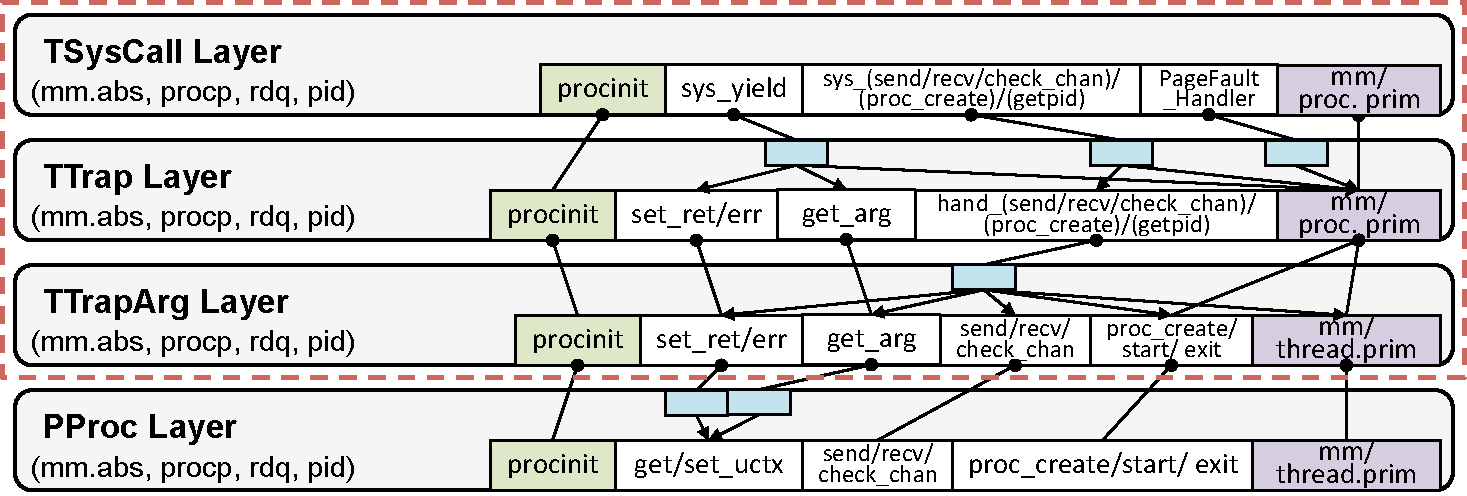
\includegraphics[scale=0.5]{figs/trap_layer_base}	
\caption{Layers of trap handler}
\label{fig:base:trap:layers}
\hrulefill
\end{figure}

{
\begin{figure}\centering
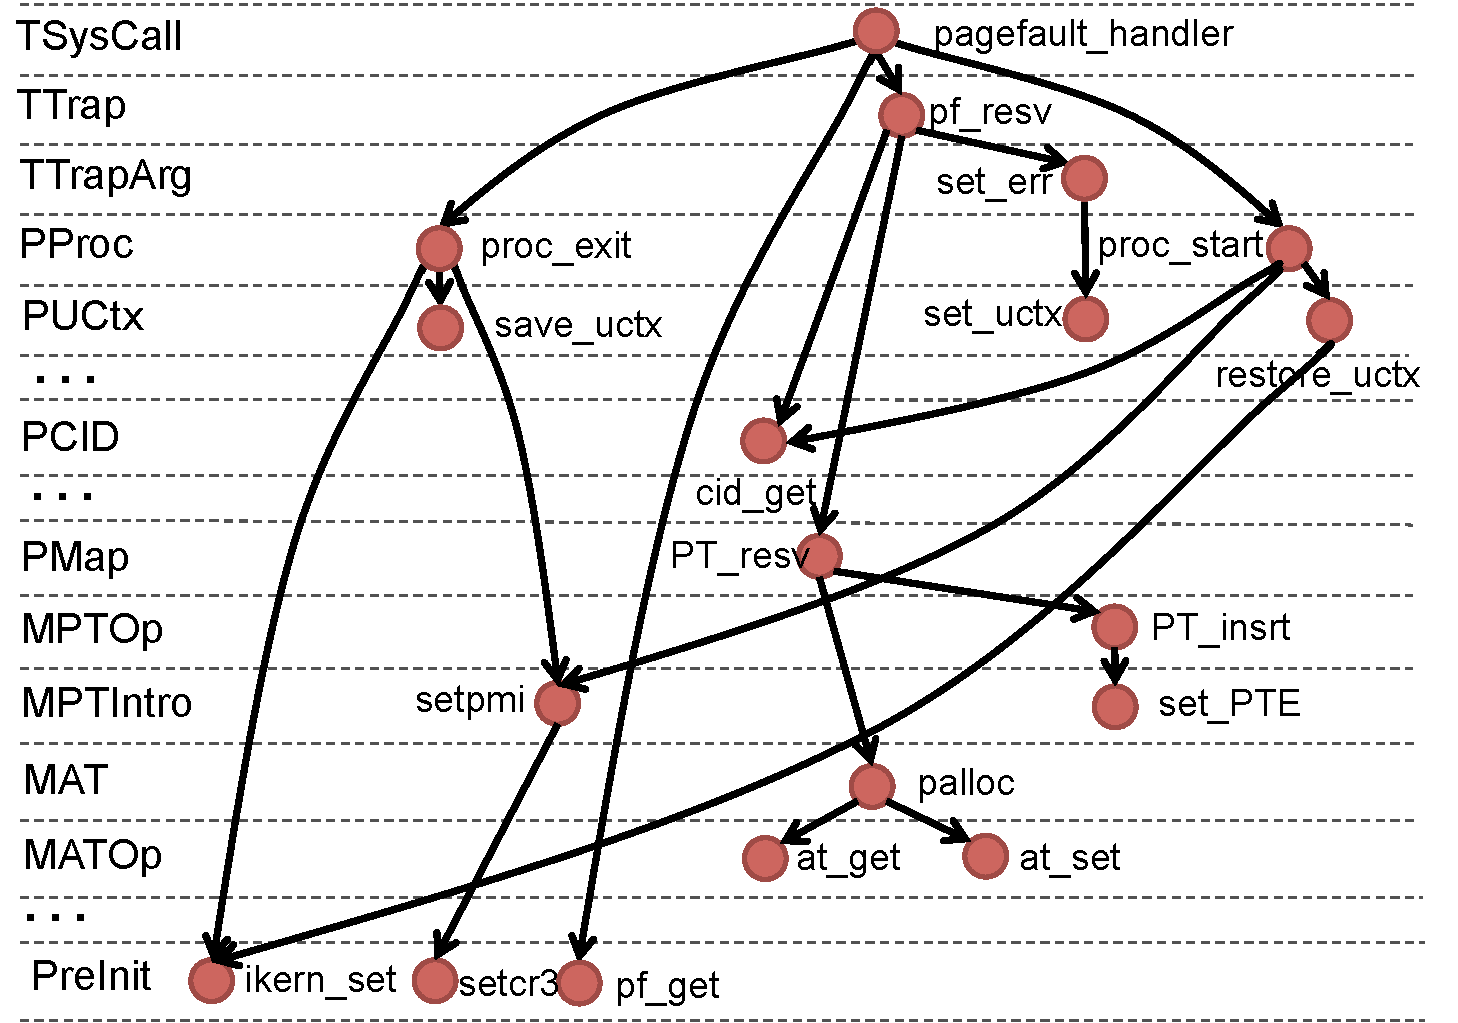
\includegraphics[scale=0.5]{figs/pagefault}	
\caption{Call graph of page fault handler}
\label{fig:base:trap:pagefault}
\hrulefill
\end{figure}
}

The trap module specifies the behaviors of exception handlers and
\mCTOSbase{} system calls.
The trap handler module of \mCTOSbase{} consists of 3 abs-kernel-fun
layers, shown in Fig\ ~\ref{fig:base:trap:layers}.  It specifies the
trap handler module in the standard operating system.  The
\verb"TTrapArg" layer introduces primitives to manage the system call
arguments and return values, while the \verb"TTrap" layer implements
the necessary handlers for system calls and exceptions.  Finally, the
\verb"TSysCall" layer specifies the semantics of system calls from the
user point of view, following the x86 system call convention.

To further simplify the reasoning about user code, we have implemented and
verified the user level system call libraries directly in the user space.
Since our machine semantics models hardware behaviors
like paging and ring switch, the specifications of user system call
libraries closely corresponds to the real execution model in the actual
hardware. With this atomic system call semantics in the user level,
the user code can be proved much more easily.

The behavior that saves and restores the trap frame (user context)
structure is modeled with the primitives \verb"proc_exit" and
\verb"proc_start".  The verified assembly implementation only saves
and restores the second half of the user context as the first half is
saved and restored by the hardware.  

In \mCTOSbase{}, exception handlers are registered in a table of first-class code pointers.
When an exception triggers (via interrupt), the kernel consults this table
and invokes the corresponding exception handler.
For example, a page fault at the user level traps into the kernel.
The page fault handler then reserves a page for PFLA (if necessary)
and returns to the user level.
The verification of the page fault handler depends on layer objects introduced
at different abstraction levels (\cf Figure~\ref{fig:base:trap:pagefault}).
We can see that the
implementation of the page fault handler involves 18 primitives across
12 layers.  On the other hand, the verification of the handler is
fairly simple as it is specified using abstract specifications of the
functions it directly calls on a layer with a very high level of
abstraction (\verb"TTrap").
Therefore, the behavior of the page fault handler is interpreted by
the concrete first-class code pointer until all the dependent layer
objects are introduced.  Then the handler code is verified and
the behavior is interpreted using its abstract atomic specification.


\ignore{
For the exception handler, we
implement the standard page fault handler which dynamically allocates
the user memory in the page table.  Fig.~\ref{fig:base:trap:pagefault}
shows the call graph of our page fault handler. 

Here, red
points are primitives at different layers, edges represent
invocations, and the primitives are called from left to right in the
order of the edges. 
}



\ignore{
\subsectskip
\subsection{User-level program}
\label{sec:base:user}
\asubsectskip

Thanks to the contextual refinement relation that we have built between the system call primitives and the underlying kernel implementations, we can reason about the user-level program with the specification of system calls and linked the proof with the one of \mCTOSbase{}.

For example, suppose we have verified that a user process $U$ linked with the system call specifications satisfy the specification $S$, which is
$$
\sem{\rm\mCTOSbase{}}{U}\Refrel{}\sem{}{S}
$$

By the final theorem of \mCTOSbase{} we have proved, 
$$
\forall P,\;\sem{\rm{}x86}{K\join{}P}\Refrel{}\sem{\rm\mCTOS}{P}
$$
, and instantiate $P$ with $U$, we can get the theorem that
$$
\sem{\rm{}x86}{U\join{}K}\Refrel{}\sem{}{S}
$$
, meaning that the user program $U$ linked with the kernel implementation $K$ and running on a x86 bare machine still satisfy the specification $S$.

%% To be moved to POPL: OSDI do not care about C vs. Asm
%%However, one limitation is that, we could not link a certified compiler using flat memory model with \mCTOSbase{}. It means that we can only verify the user-level program at assembly level instead of at C level.

\ronghui{
\begin{itemize}
\item Maybe we can find some interesting user programs
%% \item We can also put the limitation to the section 7. --> moved to POPL
\item where to put the final theorem
\end{itemize}
}
}
    % Case study: certified OS kernels (1 page)
\chapter{Concurrent CertiKOS Framework}
\label{chap:con}

In this Chapter, we will show how to
extend the sequential \CTOS{} framework
with the global log
to support concurrent program reasoning.
Section~\ref{sec:layer} introduces
the concurrent abstract machine with
global log, which extends the layer calculus
to support concurrent abstraction layers.
In Section~\ref{sec:mach},
we show a chain of concurrent
machine models from
multicore hardware machine
to a CPU-local machine.
Therefore,  most of the concurrent code
can be verified similar to sequential code,
making it possible to reuse lots of tools
developed in the sequential \CTOS{} framework.
\ignore{In Section~\ref{sec:comp},
we show how to equip CompCertX
with algebraic memory model to form a verified \emph{thread-safe} C compiler.}

%\section{Informal Development}
\label{sec:informal}

In this section, we give an overview of a few high-level ideas on how
we build certified concurrent layers. 

Like a sequential layer~\cite{dscal15}, each concurrent layer can also
contain thread-private abstract states (refined from the concrete
thread-local in-memory data) and related abstract primitives. However,
the data shared by multiple threads are not represented as abstract
states. Instead, each method call to a shared atomic object is
recorded as an observable event and is appended to the end of a shared
global log. For each shared object, we define a {\em replay} function
that can reconstruct the current shared state from the current global
log. Thus, all shared objects are represented as a single sequence of
logged events with appropriate replay functions.

With concurrency, the machine semantics for each layer (e.g.,
$\sem{L}{\cdot}$) is no longer deterministic: for each scheduler
strategy ($\strat{hs}$), it may generate a different global
log. To prove the simulation $\sem{L'}{P\oplus{}M} \leq_R \sem{L}{P}$,
for each scheduler strategy $\strat{hs}$, if running $P\oplus{}M$ on
machine $L'$ with $\strat{hs}$ produces a global log $l$, we must find
another scheduler strategy $\stratp{hs}$ such that running $P$ on
machine $L$ under $\stratp{hs}$ would generate a global log $l'$ that
is related to $l$ via the simulation relation $R$. We will actually
construct a {\em function} that will map $l$ and $\strat{hs}$ into
$l'$ and $\stratp{hs}$. Of course, the simulation relation $R$ over
thread-private states might still be a relation~\cite{dscal15}.

\paragraph{An example of concurrent layers}
The example in Figure~\ref{fig:exp:ticket_lock_example} contains a
client program $P$ which has two threads running on two different
CPUs; each thread makes one call to the atomic primitive $\comm{foo}$
provided by the layer interface $L_3$.

Concurrent object module $M_2$ implements the layer interface $L_3$
but it is built on top of $L_2$.  The $\comm{foo}$ method calls two
atomic primitives $f$ and $g$ in a critical section protected by a
ticket lock~\cite{mcs91}.

%%%%%%%%%%%%%%%%%%%%%%%%%%%%%%
\begin{figure}
\lstinputlisting [language = C, multicols=2] {source_code/ticket_lock_example.c}
%\vspace{-5pt}
\caption{Building certified concurrent layers over a ticket lock}
\label{fig:exp:ticket_lock_example}
\vspace{-10pt}
\end{figure}
%%%%%%%%%%%%%%%%%%%%%%%%%%%%%%

The ticket-lock module $M_1$ is built on top of $L_1$ and it
implements $L_2$. Even though the implementation of a ticket lock
contains two shared integer value fields: $\comm{ticket}$ and
$\comm{now}$ (where $\comm{now} \leq \comm{ticket}$ always holds), the
interface $L_1$ only provides the atomic primitives such as
fetch-and-incrementing the $\comm{ticket}$ value, getting the current
$\comm{now}$ value, holding the lock (if the $\comm{now}$ value is
equal to the $\comm{ticket}$ value), and incrementing the $\comm{now}$
value (to release the lock). The current $\comm{ticket}$ and
$\comm{now}$ values can be reconstructed by replaying the global log
(for the $L_1$ machine).  $L_1$ also provides the atomic $\comm{f}$
and $\comm{g}$ events which are later passed on to $L_2$.

\paragraph{Strategy, environment context, and layer simulation}
Our goal is to show that for each run of $P\oplus{}M_2\oplus{}M_1$
over $L_1$, we can find another run of $P$ over $L_3$ so that the
global logs produced by both runs are related.
To show how we accomplish this, here is
a global log $l_{g1}$ produced from  
a specific run of $P\oplus{}M_2\oplus{}M_1$ over $L_1$.

\vspace*{-1ex}
% \colorbox{Peach}{\textcolor{white}{a}}
\begin{small}
\[
\begin{array}{l}
\ssame \cons (1.\incticket) \cons
\sdiff \cons (2.\incticket) \cons
\ssame \cons (2.\getnow) \cons
\sdiff \cons (1.\getnow) \cons
\ssame \cons (1.\holdlock) 
\\
\cons 
\sdiff \cons (2.\getnow) \cons
\sdiff \cons (1.\comm{f}) \cons
\sdiff \cons (2.\getnow) \cons
\sdiff \cons (1.\comm{g}) \cons
\ssame \cons (1.\incnow) 
\\
\cons \sdiff \cons (2.\getnow) \cons
\ssame \cons (2.\holdlock) \cons
\ssame \cons (2.\comm{f}) \cons
\ssame \cons (2.\comm{g}) \cons
\ssame \cons (2.\incnow) 
\end{array}
\]
\end{small}%

Throughout this paper, we assume that all programs always
start from CPU 1, and before each CPU executes an atomic primitive,
it always yields to the hardware scheduler ($hs$).
We use $\ssame$ to denote a hardware yield to the same CPU,
and $\sdiff$ for a yield to a different CPU; each such symbol
is actually an abbreviation of two consecutive switch events: switch
from CPU $i$ to $hs$ (\ie, $i\switch{}hs$), and then switch from $hs$
to CPU $j$ (\ie, $hs \switch j$).  For example, starting from CPU 1,
$\sdiff$ is an abbreviation of $(1\switch{}hs) \cons (hs\switch 2)$.

We define $\comm{target}(l)$ as the switching destination of the last event in
the log $l$, which can be either 1, 2, or $hs$. The above run,
which produced the global log $l_{g1}$, can be viewed as combining
the following {\em strategies} defined for each CPU and $hs$:

\vspace*{-1ex}
\begin{small}
\[
\strat{j} (l)=
\begin{cases}
  j.e & \text{if } (\comm{target}(l) = j) ~~\wedge \\
      & ~~~~~(l\cons (j.e)) |_{j,hs} \text{ is a prefix of } (l_{g1} |_{j,hs}) \\
\comm{undefined } & \text{otherwise}
\end{cases}
\]
\end{small}%

\noindent{}Here, $l |_{j,hs}$ only keeps those events in $l$ that are
related to participants $j$ and $hs$.  For the hardware scheduler's
strategy $\strat{hs}$, this filtering essentially means that
regardless how the CPUs (or threads) are going to play in the interim,
$hs$'s moves will always follow $l_{g1}$.  Because $\strat{hs}$
defines how switching between different CPUs is done, when we define
each CPU's strategy, we filter out other CPUs' events but still keep
those events related to $hs$.

At each step, depending on the destination ($j$) of the current log
($l$), we can query the corresponding strategy $\strat{j}(l)$ to get the
next move for $j$.  For example, if the destination is $hs$, that is,
the log ends with $(\any\switch hs)$, then it is the
hardware scheduler's turn to generate a switch event $(hs\switch \any)$.

These strategies also form a nice decomposition of the global log
$l_{g1}$. To reason about CPU 1 alone, we only need to construct
its environment context $\oracle_1 := \strat{hs} \bigcup \strat{2}$.

The layer interface $L_2$ introduces the $\acq$ and $\rel$ primitives
which trigger events $\acq$ and $\rel$ respectively. Running
$P\oplus{}M_2$ over $L_2$ could produce the following shared log $l_{g2}$:

\vspace*{-1ex}
\begin{small}
\[
\begin{array}{l}
\ssame \cons (1.\acq) \cons
\ssame \cons (1.\comm{f}) \cons
\ssame \cons (1.\comm{g}) \cons
\ssame \cons (1.\rel) 
\\
\cons \sdiff \cons (2.\acq) \cons
\ssame \cons (2.\comm{f}) \cons
\ssame \cons (2.\comm{g}) \cons
\ssame \cons (2.\rel) 
\end{array}
\]
\vspace{-5pt}
\end{small}%

The layer interface $L_3$ introduces the atomic $\comm{foo}$
primitive. Running $P$ over $L_3$ could produce the following shared log
$l_{g3}$:
\vspace*{-1ex}
\begin{small}
\[
\ssame \cons (1.\comm{foo})
\cons \sdiff \cons (2.\comm{foo})
\]
\vspace{-7pt}
\end{small}%

To build a simulation, we want to define a function mapping one
layer's log and environment context into those of another layer.  For
example, the function $f_l$, mapping a log over $L_1$ into one over
$L_2$, can be defined as follows: (1) it maps the $\holdlock$ and
$\incnow$ events in $L_1$ to $\acq$ and $\rel$ events in $L_2$; (2) it
drops the $\incticket$ and $\getnow$ events; 
and (3) it merges all the adjacent switch symbols (\eg,
$\ssame \cons \sdiff$ is merged into $\sdiff$).
The following shows that $l_{g2} = f_l (l_{g1})$ is true:

\vspace*{-1ex}
\begin{small}
\[
\begin{array}{l}
\hspace*{-1em}\mysout
{\ssame \cons (1.\incticket) \cons
\sdiff \cons (2.\incticket) \cons
\ssame \cons (2.\getnow) \cons
\sdiff \cons (1.\getnow) \cons
}
\ssame \cons (1.\cancel{\holdlock}/\acq) 
\\
\hspace*{-1em}\mysout
{\cons 
\sdiff \cons (2.\getnow) \cons
\sdiff 
} 
\ssame \cons (1.\comm{f}) \cons
\mysout
{\sdiff \cons (2.\getnow) \cons
\sdiff
}
\ssame \cons (1.\comm{g}) \cons
\ssame \cons (1.\cancel{\incnow}/\rel) 
\\
\hspace*{-1em}\cons \sdiff 
\mysout
{\cons (2.\getnow) \cons
\ssame 
}
\cons (2.\cancel{\holdlock}/\acq) \cons
\ssame \cons (2.\comm{f}) \cons
\ssame \cons (2.\comm{g}) \cons
\ssame \cons (2.\cancel{\incnow}/\rel) 
\end{array}
\]
\end{small}

From $f_l$, we can construct a function $f_{\strat{}}$
that maps each strategy $\strat{j}$ for $L_1$ into one for $L_2$:

\vspace*{-1ex}
\begin{small}
\[ 
f_{\strat{}}(\strat{j}) (l'')=
\begin{cases}
j.e' & \text{if } 
\exists l', f_l(l') = l'' \wedge \strat{j}(l') = j.e\\
&\qquad\ \wedge f_l(l'\cons(j.e)) = l'' \cons (j.e') \\
\comm{undefined } & \text{otherwise}
\end{cases}
\]
\end{small}

Here, since many $L_1$ events are dropped in $L_2$,
the $L_2$ strategy $f_{\strat{}}(\strat{j})$ for $j$
has to keep querying $\strat{j}$ until
it also returns an event from $j$ at $L_2$.  For example, let $l'$ be
$\ssame \cons (1.\incticket) \cons \sdiff \cons (2.\incticket) \cons
\ssame \cons (2.\getnow) \cons \sdiff \cons (1.\getnow) \cons \ssame$,
since $\strat{1} (l') = 1.\holdlock$ and $f_l(l') = \ssame$, we have
$f_{\strat{}}(\strat{1}) (\ssame) =1.\holdlock$.

Finally, from $f_{\strat{}}$ we can construct the function
$f_{\oracle}$ which will map each environment context $\oracle$ for
$L_1$ into one for $L_2$.

\paragraph{Layer verification and composition}
Reasoning about a concrete strategy is simple, but when we verify
a concurrent module, we cannot assume such a specific environment context.
Instead, to verify
a layer running on CPU~$i$, we have to show that its implementation
meets its specification for all possible environment contexts
$\oracle_i$ that satisfy its ``rely'' invariants.

For example, to show that $\ltyp{L_1[1]}{R}{M_1}{L_2[1]}$, we must
show that the implementation of $\acq$ meets its specification.
This requires us to prove the starvation-freedom of the ticket
lock algorithm. To do so, we can impose the following rely conditions
over $\oracle_1$:
%%%%%%
\begin{itemize} \itemsep 0pt
\item ($\comm{INV}_{hs}$):  $\strat{hs}$ is \emph{fair}, that is,
  for any CPU $i$, the gap between two $(hs \switch i)$ events
  in the log is less than some constant $m$.
%%%%%%%
\item ($\comm{INV}_{2}$):  $\strat{2}$ will eventually release the
  lock it held, that is, the number of events generated by CPU~2
  between $(2.\holdlock)$ and $(2.\incnow)$   is less
  than some constant $n$ .
\end{itemize}
%%%%
Therefore, when CPU~1 acquires the lock, the loop iteration (\cf
line 17 in Fig~\ref{fig:exp:ticket_lock_example}) is bound by
$n \times m$, because CPU~2 can generate at most $n$ events before
releasing the lock and $\strat{hs}$ is fair to CPU~2.

Interestingly, we do not need
to prove that CPU~1 \emph{guarantees} to release the lock within $n$
steps in machine $L_2[1]$
when we prove $\ltyp{L_1[1]}{R}{M_1}{L_2[1]}$.  We can restore
this guarantee proof when we prove $\ltyp{L_2[1]}{R}{M_2}{L_3[1]}$
since clearly, each call to $\acq$ in $M_2$ is followed by a call to
$\rel$ within three steps.

Two certified layers are allowed to compose only if each one's guarantee
implies the other's rely. We cannot parallel-compose
$\ltyp{L_1[1]}{R}{M_1}{L_2[1]}$ and $\ltyp{L_1[2]}{R}{M_1}{L_2[2]}$;
but we can first get $\ltyp{L_1[1]}{R}{M_1\oplus{}M_2}{L_2[1]}$ and
$\ltyp{L_1[2]}{R}{M_1\oplus{}M_2}{L_2[2]}$, and then compose these to
get $\ltyp{L_1[T]}{R}{M_1\oplus{}M_2}{L_2[T]}$.






  % Informal Development (1.5 pages)
\section{Concurrent Abstraction Layers}
\label{sec:layer}

Following \cite{dscal15},
we understand abstraction layers
in terms of languages and program transformations,
and this is the starting point
of our formalization.
We use the following kind of abstract machine.

\begin{definition}[Machine]
A \emph{machine} is a tuple $\Mach = (S, \rightarrow, I, F)$
where $S$ is a set of states,
$\rightarrow \, \subseteq S \times S$ is a transition relation,
$I \subseteq S$ is a set of initial states, and
$F \subseteq S$ is a set of final states.
\end{definition}

\ignore{
\begin{definition}[Safety]
Given a machine $\Mach$,
we say that $s \in S$ is a \emph{stuck state}
if $s \notin F$ and there is no $s'$ such that $s \rightarrow s'$.
Then, a \emph{safe state} is a state $s$ such that there is no
stuck state $s'$ with $s \rightarrow^* s'$.
%A \emph{safe machine} is a machine which has at least one initial state,
%and for which all initial states are safe.
\end{definition}
}

\begin{definition}[Refinement]
We say that {\small$\Mach_1$} refines {\small $\Mach_2$}
and write {\small $\Mach_1 \refines \Mach_2$}
if there is a simulation relation {\small $R \subseteq S_1 \times S_2$}
such that:
\begin{itemize}
\item for any $s_1 \in I_1$,
	%if $I_2$ is non-empty then
	there exists an $s_2 \in I_2$
	such that $s_1 \ R\ s_2$;
\item for any related states $s_1\ R\ s_2$, % with $s_2$ safe,
	if $s_1 \in F_1$ then $s_2 \in F_2$ as well;
\item for any related states $s_1\ R\ s_2$, % with $s_2$ safe,
	if there is a step $s_1 \rightarrow s_1'$ in $\Mach_1$,
	then there is a series of steps $s_2 \rightarrow^+ s_2'$ in $\Mach_2$
	such that $s_1'\ R\ s_2'$.
\end{itemize}
\end{definition}

Based on these definitions,
we can make precise our notion of languages and
certified program transformations.

\begin{definition} \label{def:certified-trans}
A \emph{language} is a set of programs $\mathbb{P}$
together with a semantics operator $\llbracket - \rrbracket$,
which gives a machine $\llbracket P \rrbracket$ for each $P \in \mathbb{P}$.

A \emph{certified transformation} between languages $\mathbb{P}_1$ and $\mathbb{P}_2$
is a function $f : \mathbb{P}_1 \rightarrow \mathbb{P}_2$ such that
$\forall P \in \mathbb{P}_1 \,.\,
\llbracket f(P) \rrbracket \refines \llbracket P \rrbracket$
\end{definition}

\subsection{Certified abstraction layers}
The setting of languages and certified program transformations
offers limited compositionality:
two transformations can be vertically composed,
corresponding to stacking abstraction layers
or sequencing the passes of a certified compiler.
To make modular verification and linking more practical, Gu et
al. \cite{dscal15} introduce the notion of \emph{layer interfaces} $L$
specifying abstract states and associated primitives,
and \emph{certified modules} $L_1 \vdash_R M : L_2$,
where a piece of code $M$
implements an \emph{overlay interface} $L_2$ on top of an
\emph{underlay interface} $L_1$ through a refinement relation $R$.
This setting supports both \emph{horizontal} and \emph{vertical} composition rules,
which can be used to decompose the implementation of a layer:

\vspace{-5pt}
{\small
\begin{mathpar}
\inferrule{
  L \vdash_R M_{1} : L_1 \\ L \vdash_R M_{2} : L_2
}{
  L \vdash_{R} M_1 \oplus M_2 : L_1 \oplus L_2
}
\end{mathpar}
\vspace{-5pt}
\begin{mathpar}
\inferrule{
  L_1 \vdash_R M : L_2 \\ L_2 \vdash_S N : L_3
}{
  L \vdash_{R \circ S} M \oplus N : L_3
}
\end{mathpar}
\vspace{-5pt}
}%

Gu et al. instantiate this basic framework for
$\text{ClightX}(L)$, a modular formal semantics for the CompCert
Clight subset of C parameterized with layer interface $L$, and
$\text{LAsm}(L)$, a modular formal semantics for the CompCert x86
assembly language. For each language, they then define
the module system's judgement as:
\begin{definition} \label{def:popl15-layers}
$L_1 \vdash_R M : L_2$ is defined as a per-function simulation
$L_2 \leqslant_R \llbracket M \rrbracket L_1$. For
  each primitive $f$ defined in $L_2$, either a primitive $f$ in $L_1$
  is defined and simulates $f$ in $L_2$, or there exists a function
  $f$ in $M$, calling primitives in $L_1$, and whose behavior
  simulates that of the primitive $f$ in $L_2$.
\end{definition}
They then prove the horizontal compositionality
property
and prove that their compositional
verification framework is sound with respect to \emph{contextual
  refinement}:

\begin{theorem}[Contextual refinement]
Let $L_1 \vdash M : L_2$ be a certified abstraction layer. Then, the
transformation $P \mapsto (M \oplus P)$ is certified in the sense of
Definition~\ref{def:certified-trans}, i.e. for any program $P$:
\[ \mathcal{L}(M \oplus P, L_1) \refines \mathcal{L}(P, L_2) \]
\end{theorem}
\noindent where, for any program 
{\small $P$, $\mathcal{L}(P, L) = (S,
\stackrel{L}{\rightarrow}, I(P), F)$} is the machine describing the
whole-program (small-step) semantics of the program $P$ when external
function calls are interpreted as primitives in $L$.

\subsection{Partial machines}

Similarly,
we define our own setting of specialized machines
with support for parallel composition.

\begin{definition}[Partial machine]
\label{def:partialm}
A \emph{partial machine} is a tuple $\Mach = (A, R, G, S, \Delta, I, F)$
where:
\begin{itemize}
\item
$A \subseteq T$ is the machine's \emph{active thread set},
\item
$R \subseteq \{ l \in \Ev^* \ |\ \kw{target}(l) \notin A \}$ is a ``rely'' log invariant,
\item
$G \subseteq \{ l \in \Ev^* \ |\ \kw{target}(l) \in A \}$ is a ``guarantee'' log invariant,
\item
$S$ is the set of \emph{local states} of $\Mach$,
\item
$\Delta : S \times G \rightarrow \mathcal{P}(S \times \Ev^*)$
specifies the \emph{local transitions},
\item
$I \subseteq S$ is the set of \emph{initial local states}, and
\item
$F \subseteq S$ is the set of \emph{final local states}.
\end{itemize}
$\Mach$ will execute with a log $l$ that always satisfies the invariant $R \cup G$.
The transition relation $\Delta$ must preserve it event by event:
\begin{small}
\[ \Delta(s, l) \ni (s', \vec{e}) \Rightarrow (\forall \vec{e}_0 \,.\, l \cdot \vec{e}_0 \sqsubset \vec{e} \Rightarrow \vec{e}_0 \in G) \wedge (l \cdot \vec{e} \in R \cup G) \]
\end{small}%
An \emph{environment context} $\Env : R \rightharpoonup \Ev$
of $\Mach$ can provide for any log $l$
which satisfies the ``rely'' invariant
a move which satisfies:
\begin{small}
\[ \Env(l) = e \Rightarrow l \cdot e \in R \cup G \]
\end{small}%
We write $\EC{\Mach}$ for the set of all environment contexts of $\Mach$.
\end{definition}

In order to provide an execution model for partial machines,
we show how a regular machine can be constructed
from a partial machine
by supplementing it with an environment context.

\begin{definition}[Instantiated partial machine]
Given a partial machine $\Mach$ and an environment context $\mathcal{E} \in \EC{\Mach}$,
we define the machine:
\begin{small}
\[ \Mach \langle \Env \rangle =
	(S \times \Ev^*, \rightarrow_\Env, I \times \{\epsilon\}, F \times \Ev^*) \,, \]
\end{small}
where the step relation $\rightarrow_\Env$ is generated by:
\begin{small}
\[
	\AxiomC{$\Delta(s, l) \ni (s', \vec{e})$}
	\UnaryInfC{$(s, l) \rightarrow_\Env (s', l \cdot \vec{e})$}
	\DisplayProof
	\quad
	\AxiomC{$\Env(l) = e$}
	\UnaryInfC{$(s, l) \rightarrow_\Env (s, l \cdot e)$}
	\DisplayProof
\]
\end{small}%
We say that $\Mach$ takes a local step when the first rule is used,
and that $\Mach$ takes an environment step when the second rule is used.
\end{definition}

Because partial machines
running at different levels of abstraction
will be run alongside different kinds of environment contexts,
simulations of partial machines are stated relative to
a function $f$ which maps
environment contexts of one machine into
environment contexts of the other.
We define them as follows.

\begin{definition}[Refinement of partial machines]
Given two partial machines $\Mach_1$, $\Mach_2$ and
a function $f : \EC{\Mach_1} \rightarrow \EC{\Mach_2}$,
we say that $\Mach_1$ refines $\Mach_2$ when:
\begin{small}
\[ \Mach_1 \refines_f \Mach_2
	\ \stackrel{\text{def.}}{\Leftrightarrow}\ 
	\forall \Env \in \EC{\Mach_1} \,.\,
		\Mach_1 \langle \Env \rangle \refines
		\Mach_2 \langle f(\Env) \rangle \]
\end{small}
\end{definition}

%\begin{definition}[Simulation of partial machines]
%We say that $M_1 \le_f M_2$ if there exists a relation
%$R \subseteq (S_1 \times \Ev^*) \times (S_2 \times \Ev^*)$
%between the (local and global) states of $M_1$ and $M_2$,
%as well as a function $f : (\Ev^* \rightarrow \Ev) \rightarrow (\Ev^* \rightarrow \Ev)$
%mapping
%environment contexts intended for $M_1$ into
%environment contexts intended for $M_2$,
%such that:
%\begin{itemize}
%\item for any local initial state $s_1 \in I_1$ there exists a local initial state $s_2 \in I_2$
%	such that $(s_1, \epsilon) R (s_2, \epsilon)$;
%\item for any related pair of states $(s_1, l_1) R (s_2, l_2)$,
%	if $s_1 \in F_1$ then $s_2 \in F_2$;
%\item for any related pair of states $(s_1, l_1) R (s_2, l_2)$,
%	if $M_1$ takes a local step $\Delta_1(s_1, l_1) \ni (s_1', \vec{e}_1)$
%	then there exists a state $(s_2', \vec{e}_2)$
%	such that $(s_1', l_1 \cdot \vec{e}_1) R (s_2', l_2 \cdot \vec{e}_2)$
%	and such that $M_2$ takes a local step $\Delta(s_2, l_2) \ni (s_2', \vec{e}_2)$;
%\item for any related pair of states $(s_1, l_1) R (s_2, l_2)$,
%	if $M_1$ takes an environment step
%	then $M_2$ takes an environment step as well,
%	and the resulting states
%	$(s_1, l_1 \cdot \mathcal{E}(l_1)) R (s_2, l_2 \cdot f(\mathcal{E})(l_2))$
%	are related.
%\end{itemize}
%\end{definition}
%
%\begin{lemma}[Instantiation preserves simulations]
%Basically, $M \le_f M' \Rightarrow M(\mathcal{E}) \le M'(\mathcal{E})$.
%\end{lemma}

Now we present two different ways in which
we can concretize the environment context of a partial machine:
(1) by providing complementary partial machines to replace environment transitions;
or (2) by replacing the environment context with nondeterministic choices.
Let us first consider the composition of partial machines.

\begin{definition}[Linked partial machine]
Given two partial machines $\Mach_1$ and $\Mach_2$ with
$A_1 \cap A_2 = \varnothing$,
whose invariants satisfy:
\begin{small}
\begin{gather*}
\{ l \in R_1 \ |\ \kw{target}(l) \in A_2 \} \subseteq G_2 \quad
\{ l \in R_2 \ |\ \kw{target}(l) \in A_1 \} \subseteq G_1 \\
\{ l \in R_1 \ |\ \kw{target}(l) \notin A_2 \} = \{ l \in R_2 \ |\ \kw{target}(l) \notin A_2 \}\,,
\end{gather*}
\end{small}%
we define the composite partial machine:
\begin{small}
\[ \Mach_1 \Join \Mach_2 =
	(A_1 \cup A_2,
	 R_1 \cap R_2,
	 G_1 \cup G_2,
	 S_1 \times S_2,
	 \Delta,
	 I_1 \times I_2,
	 F_1 \times F_2) \,. \]
\end{small}%
The local transition relation is defined as:
\begin{small}
\begin{align*}
\Delta(s_1, s_2, l) =
	&\ \{ (s_1', s_2, \vec{e}) \ |\ (s_1', \vec{e}) \in \Delta_1(s_1, l) \} \\ \cup
	&\ \{ (s_1, s_2', \vec{e}) \ |\ (s_2', \vec{e}) \in \Delta_2(s_2, l) \} \,,
\end{align*}
\end{small}
\end{definition}

The linking operator replaces some of the environment steps of one machine
with local steps of the other.
It preserves simulations in the following sense:

\begin{lemma}[Monotonicity of $\Join$]
\label{lemma:mono}
Given $\Mach_1 \refines_f \Mach_1'$ and $\Mach_2 \refines_f \Mach_2'$ we have
$\Mach_1 \Join \Mach_2 \refines_f \Mach_1' \Join \Mach_2'$.
%\begin{proof}
%TODO: prove.
%\end{proof}
\end{lemma}

The other way $\Env$ can be concretized
is to let it range over all environment contexts
and to build a nondeterministic machine.
This is useful when the environment
does not contain any concurrent threads,
but only the hardware scheduler.

\begin{definition}[Nondeterminized partial machine]
Given a partial machine $\Mach$,
we define the machine:
\begin{small}
\[ \bigcup \Mach =
	(S \times \Ev^*, \textstyle\bigcup\nolimits_{\mathcal{E} \in \EC{\Mach}} \rightarrow_\mathcal{E},
		I \times \{ \epsilon \}, F \times \Ev^*) \,, \]
\end{small}%
where $\rightarrow_\mathcal{E}$ is defined as before.
\end{definition}

\begin{lemma}[Monotonicity of $\bigcup \Mach$]
\begin{small}
\[ \Mach_1 \refines_f \Mach_2 \Rightarrow \bigcup \Mach_1 \refines \bigcup \Mach_2 \]
\end{small}
%\begin{proof}
%\end{proof}
\end{lemma}

\subsection{Putting it together}

Since linking operates in the setting of partial machines
while the module system operates in its own setting,
we need to connect them
via the common setting of (regular) machines and refinements.

Consider a fixed program $P$
from which we build two partial machines $\Mach_1$ and $\Mach_2$.
$\Mach_2$ corresponds to an execution of the program
on top of a high-level specification of the subsystem
we with to verify,
whereas $\Mach_1$ runs the program $P$ together with the subsystem's implementation $M$
on top of a low-level machine.
Both machines execute a number concurrent threads $t \in T$.

In a first verification step,
we use the setting of partial machines and partial machine refinements to 
decompose $\Mach_1$ and $\Mach_2$ on a per-thread basis
by expressing them as linked machines:
\begin{small}
\[
	\Mach_1 \refines_\id \bigJoin_{t \in T} \Mach_1^t  \hspace{3em}
	\bigJoin_{t \in T} \Mach_2^t \refines_\id \Mach_2
\]
\end{small}%
Thanks to Lemma~\ref{lemma:mono},
it is sufficient to show that for each thread $t$:
\begin{small}
\[
		\Mach_1^t \refines_f \Mach_2^t \,
\]
\end{small}%
We expand the definition of $\refines_f$
to move back to the setting of regular machines,
so that we now need to prove for each thread $t$:
\begin{small}
\[
	\forall \Env \in \EC{\Mach_1^t}\,.\,
		\Mach_1^t \langle \Env \rangle \refines
		\Mach_2^t \langle f(\Env) \rangle
\]
\end{small}%
Then, in order to prove this per-thread property,
we carefully define a pair of layer interface specifications
$L_1(t, \mathcal{E})$ and $L_2(t, \mathcal{E}')$,
parametrized by a thread identifier and an environment context,
so that the following refinements hold for all $t, \mathcal{E}, \mathcal{E}'$:
\begin{small}
\begin{gather*}
	\Mach_1^t \langle \Env \rangle \refines \kw{LAsm}(L_1(t, \Env), P \oplus M) \\
	\kw{LAsm}(L_2(t, \Env'), P) \refines \Mach_2^t \langle \Env' \rangle
\end{gather*}
\end{small}%
If we can show that
$ \ltyp{L_1(t, \mathcal{E})}{R}{M}{L_2(t, f(\mathcal{E}))} $,
then the soundness theorem of the module system
can be used to bridge the remaining gap.


     % Concurrent Abstraction Layers (1.5 pages)
\newcommand{\PBoot}{\mathsf{PBoot}}
\newcommand{\XAsm}{\mathsf{XAsm}}

\section{Concurrent Machine Chain}
\label{sec:mach}

\ignore{
\paragraph{outline} 1) C-level vs assembly-level programming
2) layer refinement for composing multiple events?
3) spinlocks (ticket lock, MCS lock)
4)thread management
5) queuing locks
6) starvation-free condition variable
}

In this section, we introduce a realistic
concurrent multiprocessor machine model $\mach{x86mc}$,
and an assembly machine $\LAsm$ with a single active CPU
and suitable concurrent layer interfaces; then, we prove
refinement between these two machines.

\subsection{Concurrent hardware machine}
Our fine-grained multicore hardware $\mach{x86mc}$
is an \emph{abstract machine} (\cf Definition~\ref{def:mach}),
which allows arbitrary
interleavings at the level of \emph{assembly instructions}.
At each step, the hardware \emph{randomly} chooses one CPU 
and executes the next assembly instruction on that CPU.


\paragraph{The machine state $\mach{x86mc}.S$} is a tuple $(c, f_\regs, m, a, l)$,
which consists of 
the current CPU $id$ $c$,
all CPUs' private states $f_\regs$
(\ie, a partial map from CPU $id$ to private state $\regs$),
a shared memory state $m$,
an abstract state $a$, and a global log $l$.
%The assembly language
%contains an extra register set component $regset$.
The private state $\regs$ consists of a CPU-local memory
(invisible to other CPUs) and a register set.

The global log $l$ 
is a list of events, which records all \emph{shared primitive calls} that affect more than
one CPU in the machine. Events generated by different CPUs are
interleaved in the log, following the actual chronological order of events.

The shared memory state  $m$ 
is \ignore{also  a sequence of
memory blocks, which are }shared among all CPUs.
Each shared memory location is associated
with a ``valid'' bit in the abstract state $a$, which can only be manipulated by 
two shared primitives called $\pull$ and $\push$. The $\pull$ operation
changes the bit from invalid to valid, after which shared memory accesses
can be performed. The $\push$ operation invalidates the bit
and records the shared memory updates to the log.
For example,
suppose
the last event in the log
is $``1.\push(i,x)"$
(\ie, CPU 1 push the value $x$ to the shared location $i$),
the memory accesses from CPU 0 to the shared location $i$
is shown as below:
\[
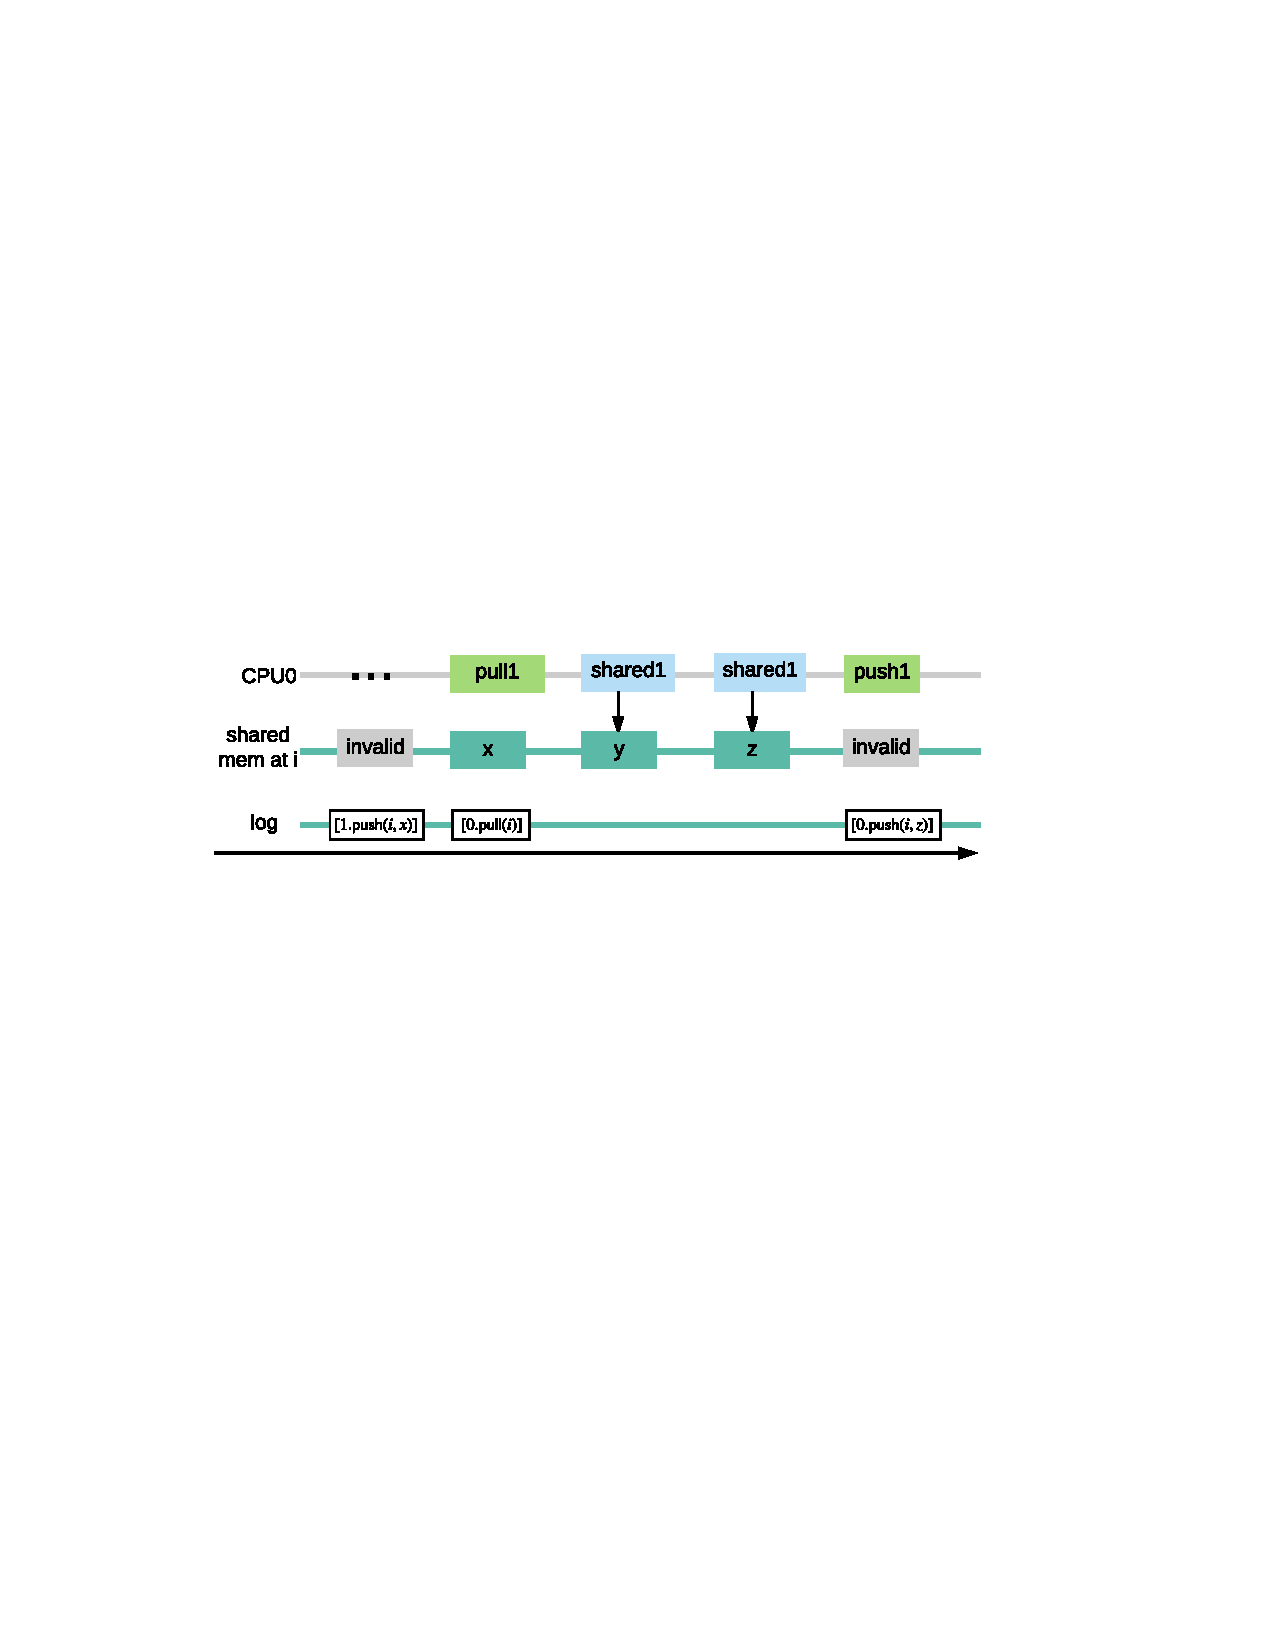
\includegraphics[scale=1]{figs/machine3}
\]
If a program tries to $\pull$ a shared memory location that is already valid,
this indicates a \emph{data race} and the machine gets \emph{stuck}.
One goal of concurrent program verification is to show
that a program is data-race free; in our setting, we accomplish 
this by showing that the program does not get stuck.

With this $\push/\pull$ model, shared memory accesses
can be treated as CPU-private executions,
whose effects to the whole machine
will be reflected by the following $\push$ operation. 

\paragraph{The transition relation $\mach{x86mc}.(\rightarrow)$}
consists of two types of transitions: 
\emph{program transitions} and \emph{hardware scheduling}, which can 
be nondeterministically interleaved.

\emph{Program transitions} can be of three types:
private transitions,
non-atomic shared transitions,
and atomic transitions.
Private transitions consist of
internal statements that only access
CPU-private memory,
and  private primitive calls.
Non-atomic shared transitions
only include 
internal statements that access shared memory.
The first two types are ``local'', 
in that they can only access CPU-private 
state and the portion of shared memory marked as valid.
In both case, the global log $l$ will not be accessed.
Atomic transitions are
shared primitives calls, 
which will access shared object
and provide the only means 
for accessing the global log and for generating events.
Both $\push$ and $\pull$ operations
are special shared primitive calls.
\ignore{
whose semantics is denoted
as the step relation $(args;s, res;s')$.
It says that starting from the state $s$ with the argument
$args$, the execution terminates with the state $s'$ and return
value $res$.}

\emph{A hardware scheduling transition} changes the
current CPU $id$ to some other $id$ 
and  can be arbitrarily interleaved with
program transitions.

This concurrent machine model $\mach{x86mc}$
reflects the nondeterministic concurrency features of 
multi-core hardware. 
One interleaving of an example program running on two CPUs
is:
\[
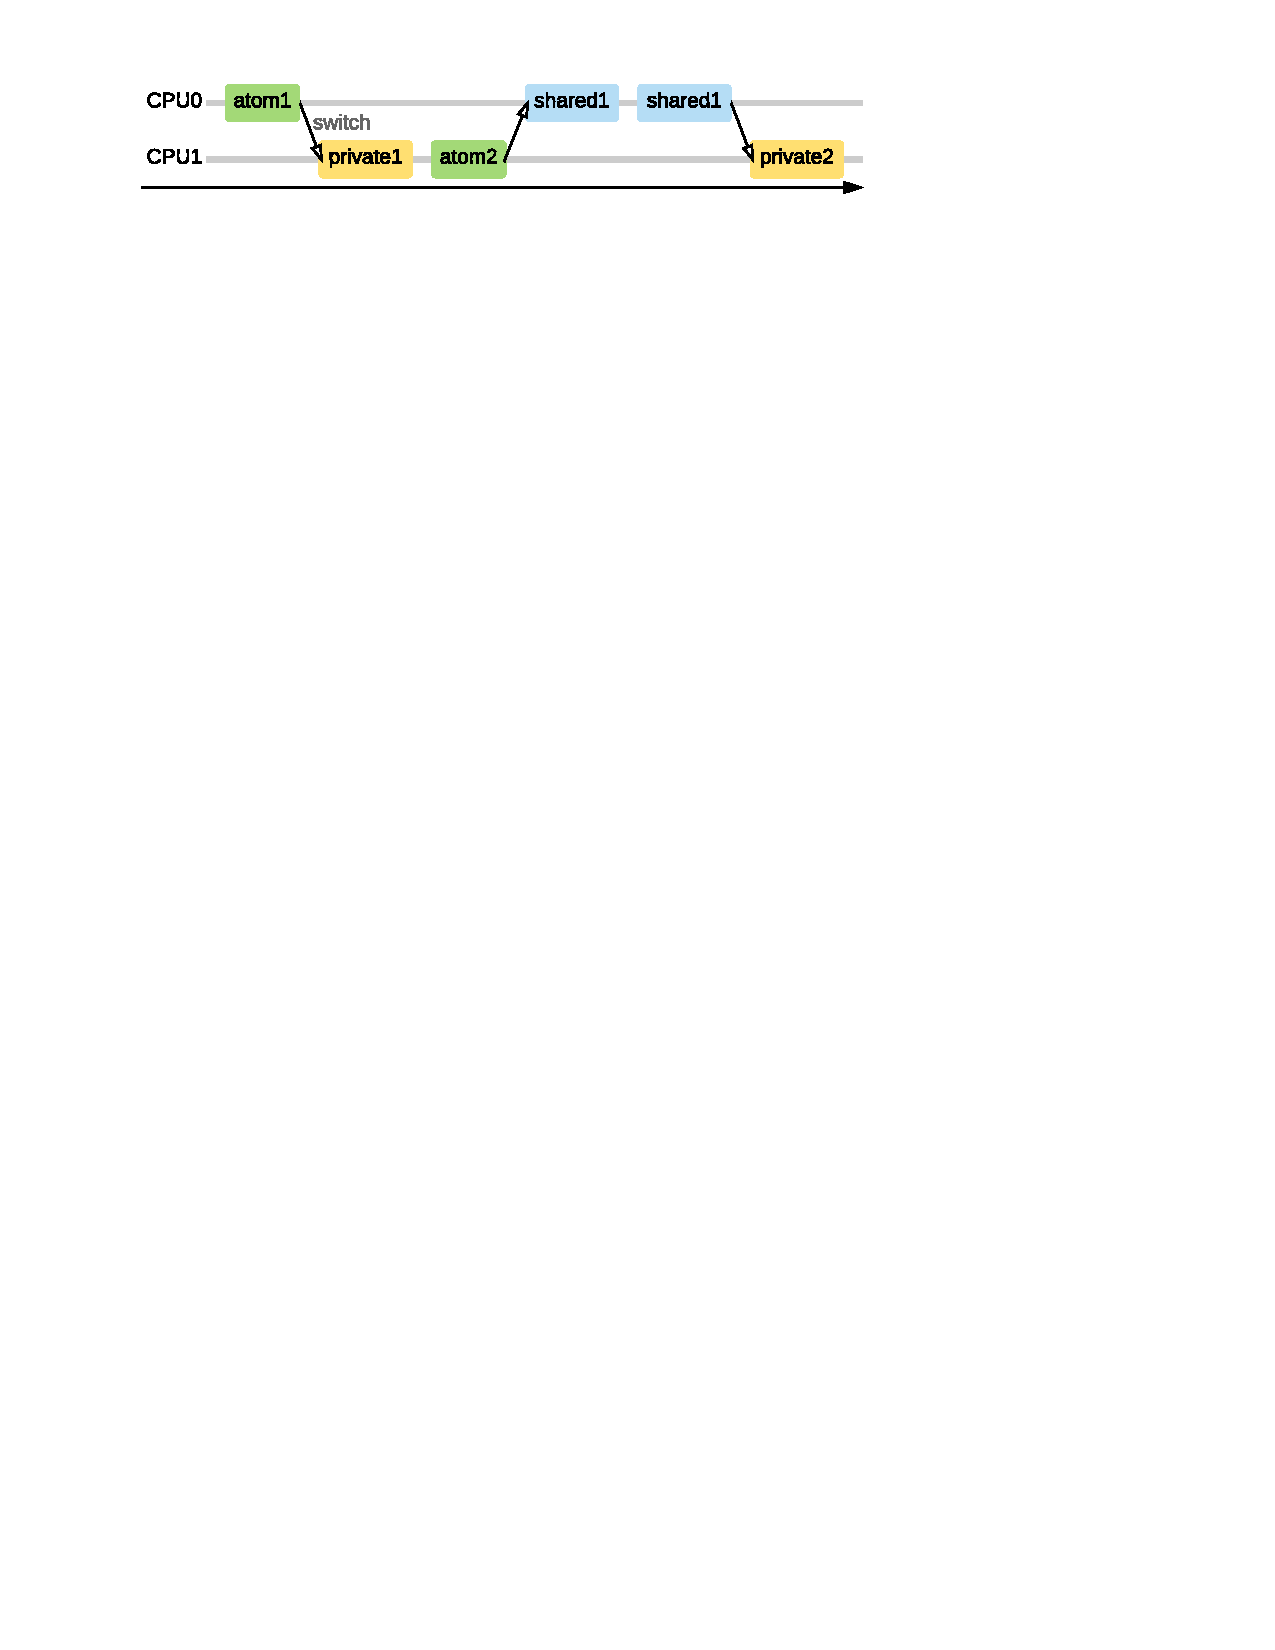
\includegraphics[scale=.93]{figs/machine1}
\]
Since only atomic transitions generate events,
this interleaving produces the logical log $[\event{0.\mathsf{atom}_1,1.\mathsf{atom}_2, 0.\pull_1,0.\push_1}]$.

\paragraph{Sequential consistency}
The \push/\pull{} memory model
assumes that the memory of the multi-core hardware
is \emph{sequentially consistent}~\cite{lamport1979make}.
Previous works~\cite{steinke2004unified,
boudol2009relaxed,owens2009better} have shown that,
for data-race free programs,
multiprocessor executions 
can be modeled as a sequence of 
shared memory access events,
which is sequentially consistent.
Therefore, by showing that the \cCTOS{}
kernel is data-race free,
we have that this sequential consistency assumption
is valid.

\subsection{Partial machine with hardware scheduler}
As a first step toward abstracting away the low-level details of
concurrent CPUs, we introduce a new partial machine ($\pmach{hs}$) configured
with a
\emph{hardware scheduler} ($\hardoracle$) that specifies a 
particular interleaving for an execution. 
This results in a deterministic machine model.
To take a program from $\mach{x86mc}$ and run it on top of $\pmach{hs}$,
we insert a  \emph{logical \intptext}
(denoted as ``$\intp$") before each assembly instruction.
Each switch point \intptext
yields to the hardware scheduler
and generates
a switch event
$c \switch hs$,
which is a \emph{local step} $\mach{hs}.\Delta$.
Then, the machine has to take
an \emph{environment step} to query the hardware scheduler
and get the CPU $id$ $c'$ to execute next.
This \emph{decision} made by $\hardoracle$ is stored in the 
log as a switch event $hs \switch c'$. 
The previous example on $\mach{x86mc}$
can be simulated by the following $\hardoracle$:\vspace{-5pt}
\[
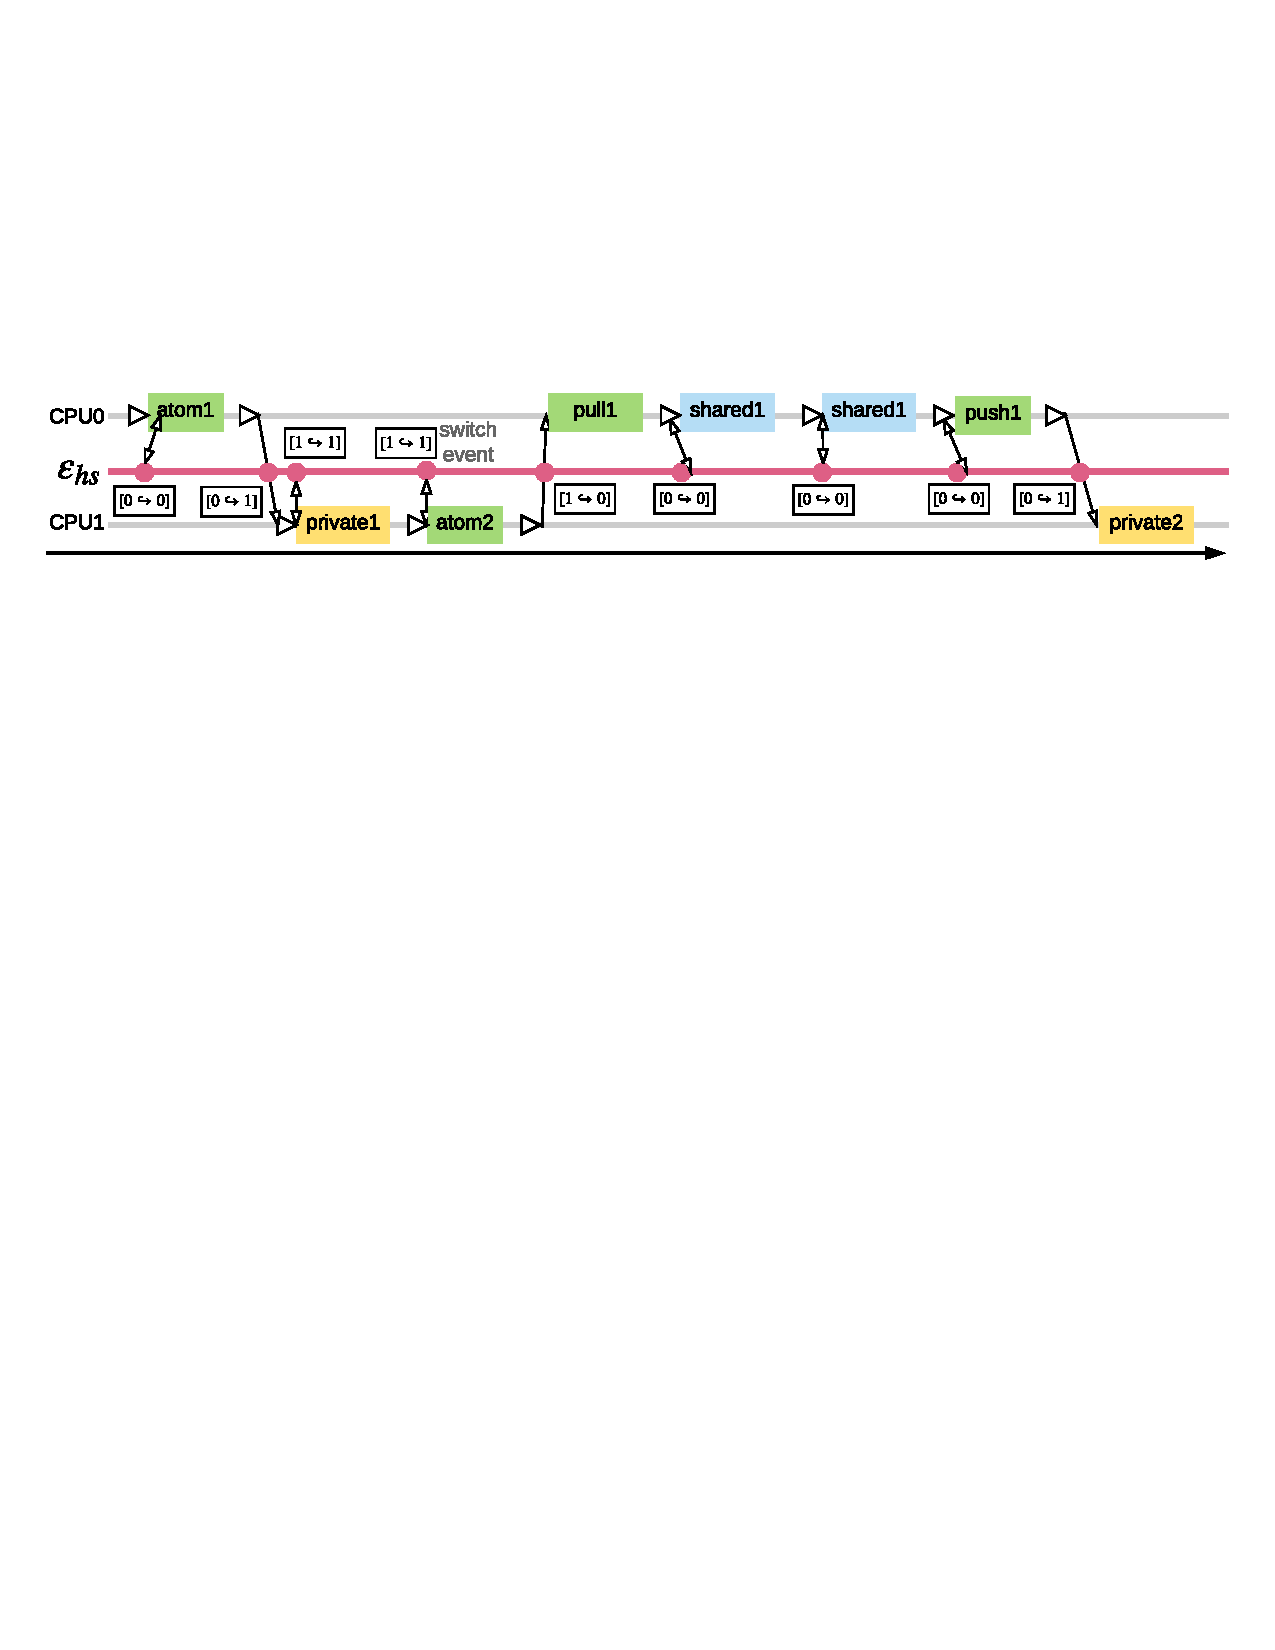
\includegraphics[scale=.75]{figs/machine2}
\]
\noindent
We write $(c \switch c')$
as an abbreviation of $(c \switch hs) \cons (hs \switch c')$.
Thus,
the log recorded by this execution is as follows:
\[
\begin{array}{l}
(0\switch 0) \cons (0.atom_1)
\cons (0\switch 1) \cons (1\switch 1)
\cons  (1\switch 1) \cons (1.atom_2)
\cons (1\switch 0) \cons (0\switch 0)
\cons ( 0\switch 1)
\end{array}
\]
\noindent
Note that this model is a special case of the partial
machine,
where the 
active set is the set of all CPUs,
and the environment is the hardware scheduler.
The \emph{rely} log invariant simply holds
on any log that the \emph{target} is $hs$:
\[\pmach{hs}.R := \{ l \in \Ev^* \ |\ \kw{target}(l) = hs \}\]
The \emph{guarantee} invariant states
two important properties:
\emph{data-race freedom}
and \emph{active consistency}.
The first property says
 that there is no
data race in the system,
\ie, there is no $\pull$ operations over $\code{valid}$
memory location and every $\push$ operation
are done following its $\pull$ operation.
The second property simply
requires that all the events
are generated by the current active CPU or the hardware scheduler.
We write $\code{well\_form}$ a predicate
over logs to state these twp properties.
Thus, the guarantee invariant is shown as below.
\[\pmach{hs}.G := \{ l \in \Ev^* \ |\ \kw{target}(l) \in \code{CPU\_set}
\land \code{well\_form}(l) \}\]
Any \emph{safe} execution of  local steps (\ie, $\pmach{hs}.\Delta$) result a log $l \in \pmach{hs}.R \cup \pmach{hs}.G$.
Thus, since the hardware scheduler only returns switch events,
the result log of any environment step still satisfies
$\pmach{hs}.R \cup \pmach{hs}.G$ regardless
of the next CPU $id$ decided by the hardware scheduler.
To ensure the correctness of this machine,
we prove that $\mach{x86mc}$ \emph{refines} this
partial machine with hardware scheduler.

\begin{lemma}[Correctness of the hardware scheduler mode]
\[\mach{x86mc} \refines \bigcup_{\oracle_{hs}}{
\pmach{hs}\langle \oracle_{hs} \rangle}
\]\proof[Proof Sketch]
For any interleaved execution on $\mach{x86mc}$, we construct
a corresponding hardware scheduler on $\pmach{hs}$.
Thus, the log of $\mach{x86mc}$
is equal to the log of $\pmach{hs}$
by removing all the switch events.
 \label{lemma:pboot}
\end{lemma}


\subsection{Partial machine with environment context}

Although $\pmach{hs}$ is deterministic
with respect to a hardware scheduler,
it still does not have much support for CPU-local reasoning.
To support modular verification, 
we should provide a \emph{partial machine}
 to reason about programs on each CPU locally by specifying
expected behaviors of the context programs on other CPUs. Thus,
we can apply the linking theorems for the partial machine
 and 
 form a global
claim about the whole system. 
To this purpose, we introduce a partial
machine model $\mach{ec}$ that can be used to reason about the
programs running on a subset of CPUs, by
parametrizing the model over the behaviors of an \emph{environment context}
(\ie, the rest of the CPUs).

The active set $A$ of the partial machine  $\pmach{ec}$
is a local subset of CPUs,
and the context contains
both other CPUs and the hardware scheduler.
At each switch point,
the machine takes an environment step
to get the next CPU $id$ to execute.
If it yields a CPU outside the active set,
it will keep taking the environment step
to get the next event generated
by the context, until yielding back to an active CPU.

\paragraph{Environment context}
of $A$ in this machine model 
is denoted as $\ectxt{\pmach{ec}^A}$.
Each environment context $\oracle_{ec}\in\ectxt{\pmach{ec}^A}$
is a \emph{response function},
which takes the current log 
and returns an event from the context CPUs
or the hardware scheduler,
which is guaranteed to satisfy some invariant.
In other words, response function simulates the observable behavior 
of the context CPUs and the potential interleaving, while the invariant states the assumptions being 
made over the context.
The execution of CPU 0 in the previous example can be simulated
with a $\oracle_{ec}$.
\ignore{$\oracle_{\overline{\set{0}}}$
(\ie, $\oracle_{\set{1}}$, since there are only two CPUs).}
\[
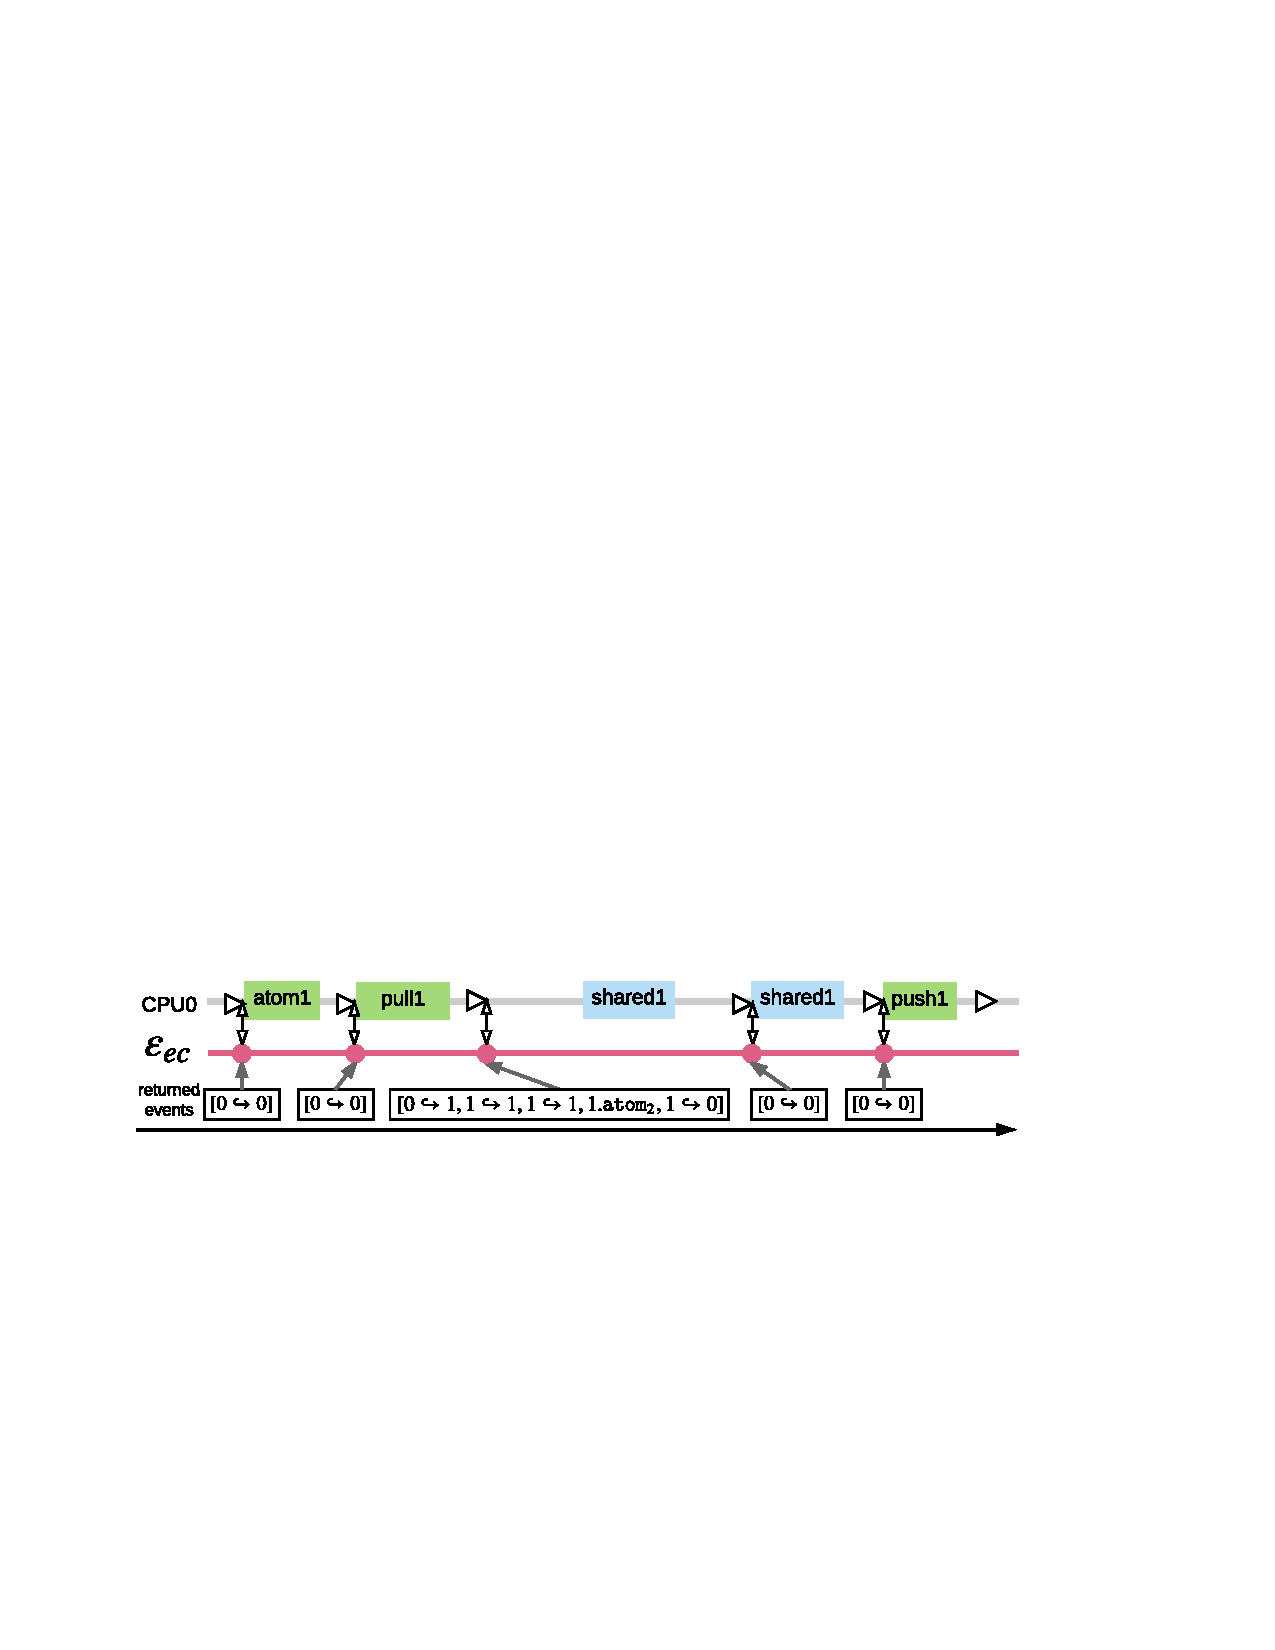
\includegraphics[scale=.9]{figs/machine4}
\]

\ignore{The environment context $\oracle_{\set{1}}$
generates the event list $[\event{0\switch 1},\event{1\switch 1},\event{1\switch 1}, \event{1.atom_2}, \event{1\switch 0}]$
at the third \intptext.}

\paragraph{Composition with environment context}
For the partial machine $\mach{ec}$,
both the rely and guarantee invariants
require the log to be well-formed.
\begin{align*}
\pmach{ec}^A.R := \{ l \in \Ev^* \ |\ \kw{target}(l) \not\in A
\land \code{well\_form}(l) \} \\
\pmach{ec}^A.G := \{ l \in \Ev^* \ |\ \kw{target}(l) \in A
\land \code{well\_form}(l) \}
\end{align*}
Therefore, for disjoint active set $A_1$ and $A_2$,
the linking operator $\Join$ is well-defined 
(\cf Definition~\ref{def:link:partial}),
and form the linked partial machine:
\[\pmach{ec}^{A_1} \Join \pmach{ec}^{A_2}
\quad \text{ if } A_1 \cap A_2 = \emptyset\]

After composing the programs on all CPUs, the context CPU set becomes
empty, and the hardware scheduler is the only context.
Since we can prove that the log generated
by any safe execution on $\mach{hs}$
is well-formed,
the environment context is  is
reduced to the \emph{hardware scheduler}
$\oracle_{hs}$, which only generates the
switch events. In other words, by
showing that this \emph{composed machine} with the entire CPU set
is refined by $\pmach{hs}$, 
all the properties proved can be propagated down to the
multicore hardware model.

\begin{lemma}[Correctness of the environment context model]
\[\pmach{hs} \refines_\id \bigJoin_{c\in\comm{CPU\_set}}
\pmach{ec}^{c}\]
\end{lemma}


\subsection{CPU-local machine}
\label{subsec:spec:seq}
If we focus on a single active CPU $i$,
the partial machine $\pmach{ec}^i$ is like a \emph{local} machine
with an environment context representing all other CPUs
and the hardware scheduler. However,
in this model there is a {\intptext} before each instruction,
so program verification still needs to handle many unnecessary 
interleavings (\eg, the ones between private operations).
In this subsection, we introduce a CPU-local
machine model (denoted as $\pmach{loc}$) for a CPU $i$, in which {\intptext}s
only appear before shared atomic operations.
The {\intptext}s before shared or private operations
are removed via two steps: \emph{shuffling} and \emph{merging}.

\paragraph{Shuffling {\intptext}s}
In $\pmach{loc}$, we introduce a \emph{log cache}~--- for
the {\intptext}s before shared and private operations,
the query results from the environment context
are stored in a temporary log cache.
The cached events are applied to the logical log
just before the next shared atomic operation.
Thus, when we perform shared or private operations,
the observations of the environment context are delayed
until the next atomic operation.
This is valid because a shared operation can only be performed
when the current local copy of shared memory is valid, meaning that 
no other context program can interfere with the operation.

\paragraph{Merging {\intptext}s} Once the {\intptext}s are shuffled properly,
we merge all the adjacent {\intptext}s together.
When we merge {\intptext}s, we also need to merge 
the switch events generated by the environment context.
For example, the change of {\intptext}s for the previous example
on CPU-local machine is as follows: 
\[
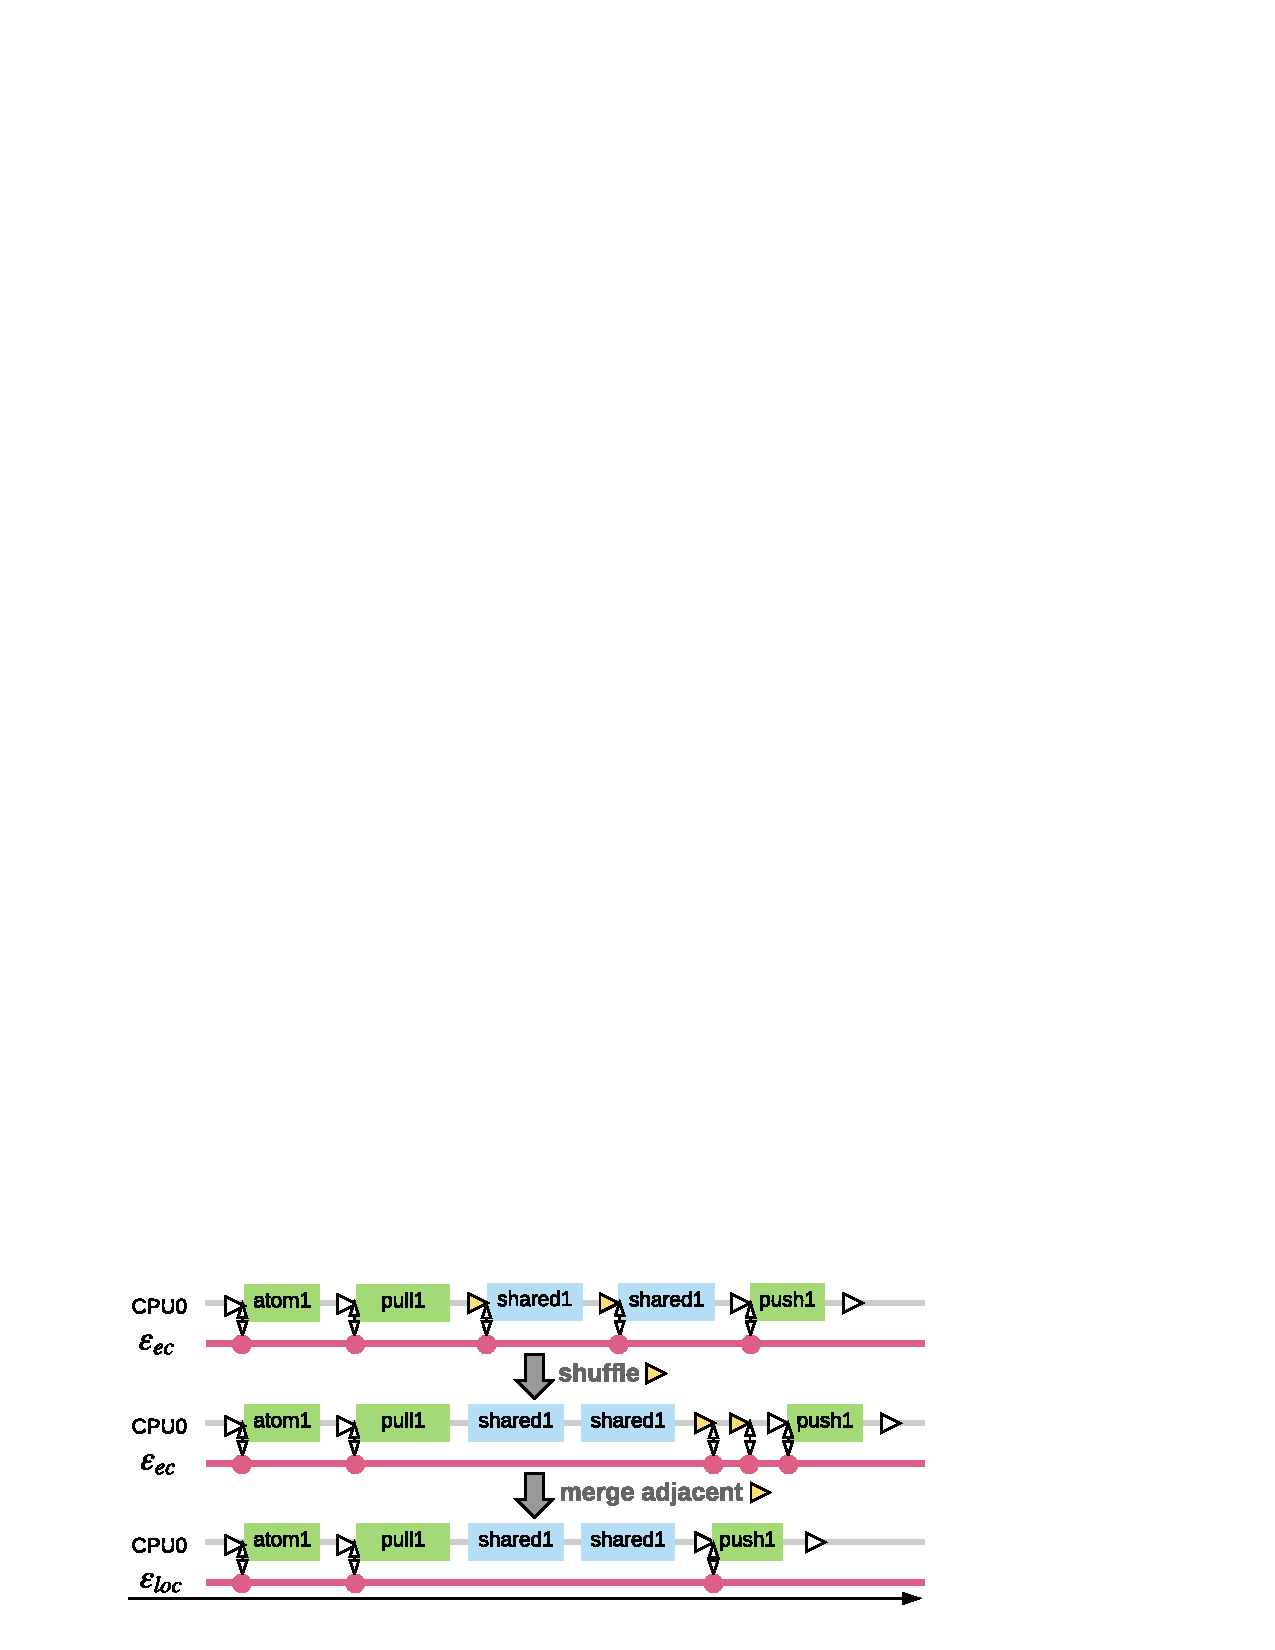
\includegraphics[scale=.9]{figs/machine5}
\]

\begin{lemma}[Correctness of CPU-local machine model]
\[\pmach{ec}^c \refines
\pmach{loc}^{c}\]

\ignore{
\[
\forall \oracle_{\overline{\set{i}}},
\exists \oracle'_{\overline{\set{i}}},
(\mach{pt},\oracle_{\overline{\set{i}}})_{\set{i}}
\machrel 
(\mach{loc},\oracle'_{\overline{\set{i}}})_{\set{i}}
\]
}
\ignore{\[
\begin{array}{l}
\forall P\ \oracle_{\overline{\set{i}}}\ \inv_{\set{i}},
\exists \oracle'_{\overline{\set{i}}},\\
\machbe{P}{\mach{pt}}{\oracle_{\overline{\set{i}}},  \inv_{\set{i}}}
\machrel 
\machbe{P}{\mach{loc}}{\oracle'_{\overline{\set{i}}}, \inv_{\set{i}}}
\end{array}
\]
\proof
Shuffling and merging {\intptext}s  are valid.
\qed}
\end{lemma}




\subsection{LAsm with concurrent layer interface}
\label{sec:con:lasm}

\ignore{
The Lemma~\ref{lemma:pboot} actually ``links'' $\PBoot$ with all
possible semantics for the hardware scheduler $hs$.}

%% Thanks to the Lemma~\ref{lemma:pboot}, the guarantees proved
%% over $\PBoot$ can be propagated down to the $\Mach_\boot$ level.

% TODO: This is wrong.
%% What's more, by the monotonicity lemma~\ref{lemma:mono},
%% we can build certified abstraction layers
%% with a single CPU $c$ on $\LAsm(L(c,\oracle))$, and compose the 
%% abstraction layers with the linking operator $\Join$.
%% In the rest of the paper, we will focus on this single-core
%% machine $\LAsm(L(c,\oracle))$.

\ignore{\paragraph{Single-core assembly machine $\LAsm(L(c,\oracle))$}}
The $\LAsm$ assembly machine model (\cf Section~\ref{sec:seq:lasm}) is
designed to ease sequential compositional reasoning. $\LAsm$ takes as
argument a sequential layer interface $L := (\abst, \primt_{\mathrm{ClightX}}, \primt_{\mathrm{LAsm}}, \invt, \mat)$
(\cf Definition~\ref{def:asm-layer}).
In the concurrent setting, we can reuse $\LAsm$ with an extended
notion of layer interface, \emph{concurrent layer interfaces}.

\begin{definition}[Multiprocessor layer interfaces]
A concurrent layer interface $L :=(\abst, \Ev, \primt_{\mathrm{ClightX}}, \primt_{\mathrm{LAsm}}, \invt, \mat)$ where 
$\Ev$ is the type for all possible events
, and, for any CPU identifier $c$ and environment 
context $\oracle$, $\primt_{\mathrm{ClightX}}(c, \oracle)$ 
and $\primt_{\mathrm{LAsm}}(c, \oracle)$ are the sets of 
available C-style and assembly-style primitives. We then write $L(c, \oracle) = ((\abst, \primt_{\mathrm{ClightX}}(c, \oracle), \primt_{\mathrm{LAsm}}(c, \oracle), \invt, \mat)$ to indicate the 
concurrent layer interface for processor $c$.
\end{definition}%
\noindent
Note $L[c]$ used in Section~\ref{sec:intro:layer}-\ref{sec:overview:concurrent}
can be viewed as a set of $L(c,\oracle)$ over any $\oracle$,
and the event type of $\oracle$ has to be consistent
with $L.\Ev$.

The $\LAsm(L(c, \oracle))$ machine state is thus defined as $\state:=(\regs, m, a, l)$,
where $\regs$ is the register set for CPU $c$,
$m$ is the memory state,
$a$ is the CPU-private abstract state,
and $l$ is the global log.
The big-step semantics of programs running on a single CPU is
almost the same with the one of LAsm,
shown in Section~\ref{sec:seq:lasm}.
Except that the machine state contains the log filed $l$,
which will not be accessed by internal steps
and non-shared primitive calls.
We write $\oracle, c \vdash L.\primt_{\mathrm{ClightX}}(i) (args,m, a, l,res,m',a',l')$ to denote
the specification of the C-style primitive
with identifier $i$,
while we write $\oracle, c \vdash L.\primt_{\mathrm{LAsm}}(j) (\regs,m, a, l,\regs',m',a',l')$ to denote
the specification of the assembly-style primitive with identifier $j$,.

Since there is a switch point $\intp$ 
in front of the shared primitive,
its semantics first query the environment context $\oracle$
with the current global log $l$
and update $l$ with the returned events generated by the environment.
We also \textbf{big-step} this query to simplify the representation,
which combines many actions.
First an switch event is
appended to the log $l$ indictating that we will interact with the
environment. Then the environment context $\oracle$ is queried
multiple times. Each time it returns an event from a CPU other than
$c$ we append that event to the log, and continue querying
$\oracle$. Finally $\oracle$ will yield back to $c$
(guaranteed by the \emph{fairness} of the hardware scheduler), and
the shared primitive call occurs.
The environment query is necessary before each shared primitive call because 
other CPUs must be given a chance to update shared state before the current 
CPU accesses it. 
\ignore{Note, however, that we do not need to worry about querying
the environment at internal statements and private primitives, since
the shared state cannot influence the behavior of these
transitions.} In the following, we will abuse notation and write
$l \cons \oracle(l)$ to mean the entire process of extending $l$ with
multiple events from other CPUs.
\ignore{which means that, starting from the log $l$, $\oracle(l)$ keeps
querying and appending events until the destination
is the current CPU $c$.}

In most cases, the execution of a primitive depends on what events have
been triggered at the switch point. 
For example, the $\pull$ primitive returns the
current state of the shared memory, which depends on what shared
memory updates from other CPUs are recorded in the global log.
To write the primitive specifications, we introduce an idiom of a
\textbf{replay function} $\replay$, which takes a
log as an argument, and interprets it to calculate the ``current
state'' of the system after those events have happened. The
result of the replay function can be an arbitrary type, corresponding
to what kind of information is needed about the shared operations.

For example, the replay function $\replay_{\comm{get\_shared}}$
reconstructs the shared memory state from the given log.
It first retrieves the last shared memory
update to location $b$ from the log $l$. If the last update is
$c.\pull(b)$, it returns $(\any, \comm{invalid})$, where $\any$ denotes
any possible value. The shared memory state returned in this case
does not matter since the $\pull$ operation invalidates the corresponding
memory block. On the other hand, if the last update
is $c.\push(b,\comm{bl})$ for some byte list $\bytelist$,
it returns $(\comm{bl}, \comm{valid})$. 
If there is no $\push$ or $\pull$ event in the log, it returns
$(\any, \comm{valid})$. We write ``$f\set{b:v}$"
to denote an update to the partial function $f$ at field $b$ 
with value $v$.
The rules for $\pull$ and $\push$ are defined as below:
\begin{small}
\begin{mathpar}
\inferrule{
   l_0 = l \cons \oracle(l) \\ 
  (\bytelist,  \comm{valid}) = \replay_{\comm{get\_shared}}(l_0, b) \\
  	m' = m \set{b: \bytelist} \\
  	a' = a \set{\perm{b}: \comm{valid}}  \\	
   l' = l_0 \cons c.\pull(b) \\ 
}{
 \oracle, c \vdash  \spec_{\pull}([b],\regs, m, a, l,\any, \regs,  m', a', l')
} 
\and
\inferrule{
  m(b) = \bytelist \\
  a.\perm{b} =  \comm{valid} \\
  a' = a \set{\perm{b}: \comm{invalid}} \\
  l' = l \cons  \oracle(l) \cons c.\push(b,\bytelist)   
}{
 \oracle, c \vdash  \spec_{\push}([b], \regs, m, a, l,\any, \regs, m, a', l')
}
\end{mathpar}
\vspace{-5pt}
\end{small}%

The $\pull$ operation requires the shared memory to be marked as valid
(after replaying the log). It first queries the environment context to update
the log, and then it updates the shared memory at location $b$ with the byte
list $\bytelist$ reconstructed from the log. This specification
captures the fact that the shared memory contents may be
modified by the environment context before the execution of
primitives. 
The $\push$ operation first gets the updated log from the environment context,
and then appends an event $c.\push(b,\bytelist)$ to the end of the log.
The operation is only defined when the permission bit is valid (\ie, the previous push
has already been pulled), and it invalidates the permission upon $\push$.

Let $L_\boot$ be the multiprocessor layer interface with the same abstract state, shared events, and primitives as in $\pmach{loc}$.
\ignore{
In general, $\LAsm(L(c, \oracle))$ is, however, not a partial machine.  For the
layer $L_0$ corresponding to primitives of $\mach{\boot}$, we have
constructed a partial machine $\XAsm(c)$ for a given core $c$ such
that:

\begin{lemma}
There exists a function $f$ such that, for any environment context $\oracle$: \[ \PBoot(\oracle) \refines \bigJoin_{c} \XAsm(c)(f(c, \oracle)) \]
\end{lemma}

\begin{lemma}
For any core $c$ and for any environment context $\oracle$: \[ \XAsm(c)(\oracle) \refines \LAsm(L_0(c, f(\oracle))) \]
\end{lemma}
\tahina{TODO: define $\XAsm$ and explain the proof}
}
Then,\ignore{For the layer $L_\boot$ corresponding to primitives of $\Mach_\boot$, } we
have proven that $\LAsm(L_\boot(c, \oracle))$ can be represented as a
partial machine, so that we can state and prove the following:
 \begin{lemma}
$ \forall \oracle.\ \pmach{loc}^c\langle \oracle \rangle \refines \LAsm(L_\boot(c, \oracle)) $
 \end{lemma}

\begin{figure}[t]\centering
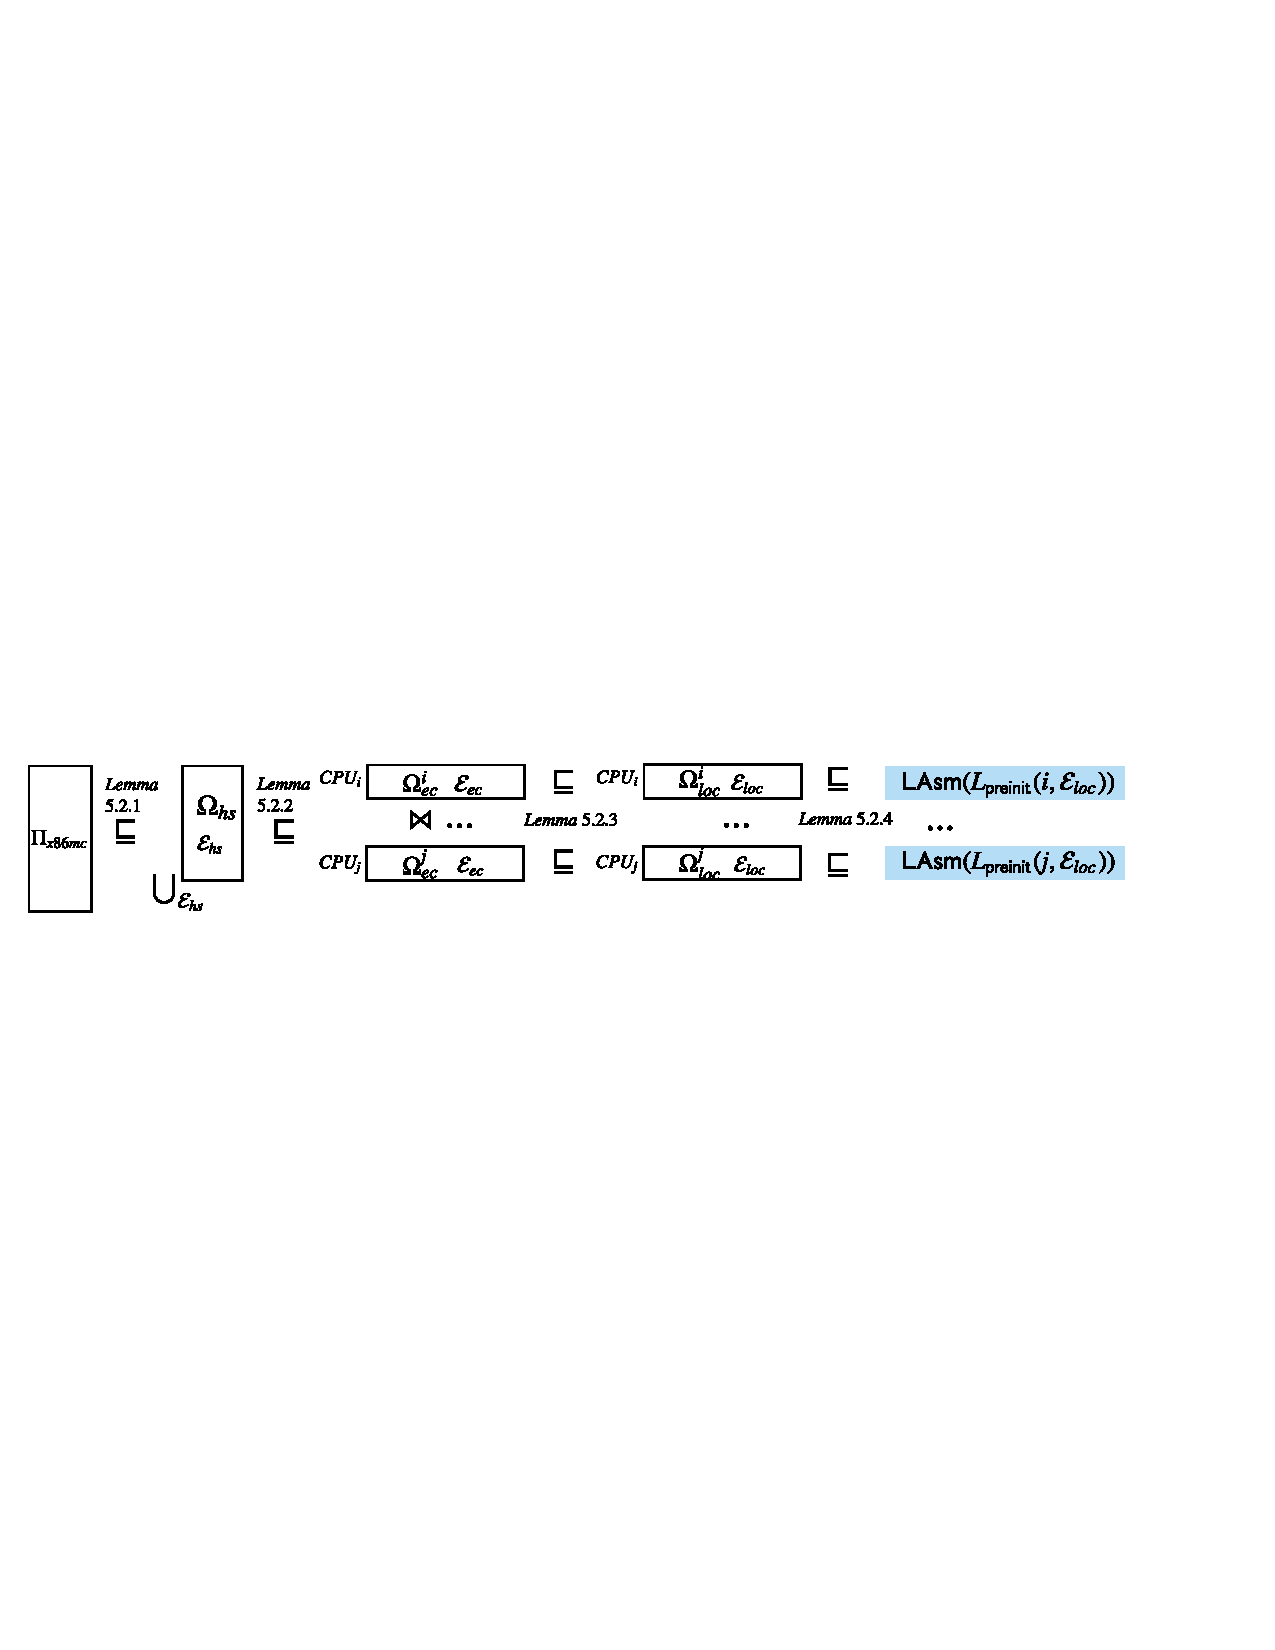
\includegraphics[scale=0.8]{figs/machine_chain}
\caption{The contextual refinement chain from multicore hardware model
$\mach{x86mc}$ to the LAsm machine
with single-core concurrent layer.}
\label{fig:spec:chain}
\hrulefill
\end{figure}

Finally, we obtain the refinement relation from the multicore
hardware model
to the single CPU LAsm machine model by composing
all of the refinement relations together (\cf Figure~\ref{fig:spec:chain}).
We introduce and verify the {\cCTOS} kernel on top of the
single CPU LAsm machine,
where the semantics of internal statements
and private primitives can be viewed as sequential,
and one only needs to consider concurrency
and interleaving at switch points (\ie, just before 
shared primitive calls).
The refinement proof guarantees that the proved properties can be
propagated down to the multicore hardware model $\mach{x86mc}$.


     % Concurrent Abstraction Layers (1.5 pages)
%%\sectskip
\vspace{-5pt}
\section{Layers with Environment Context}
\label{sec:machine}


\begin{figure}
\begin{center}
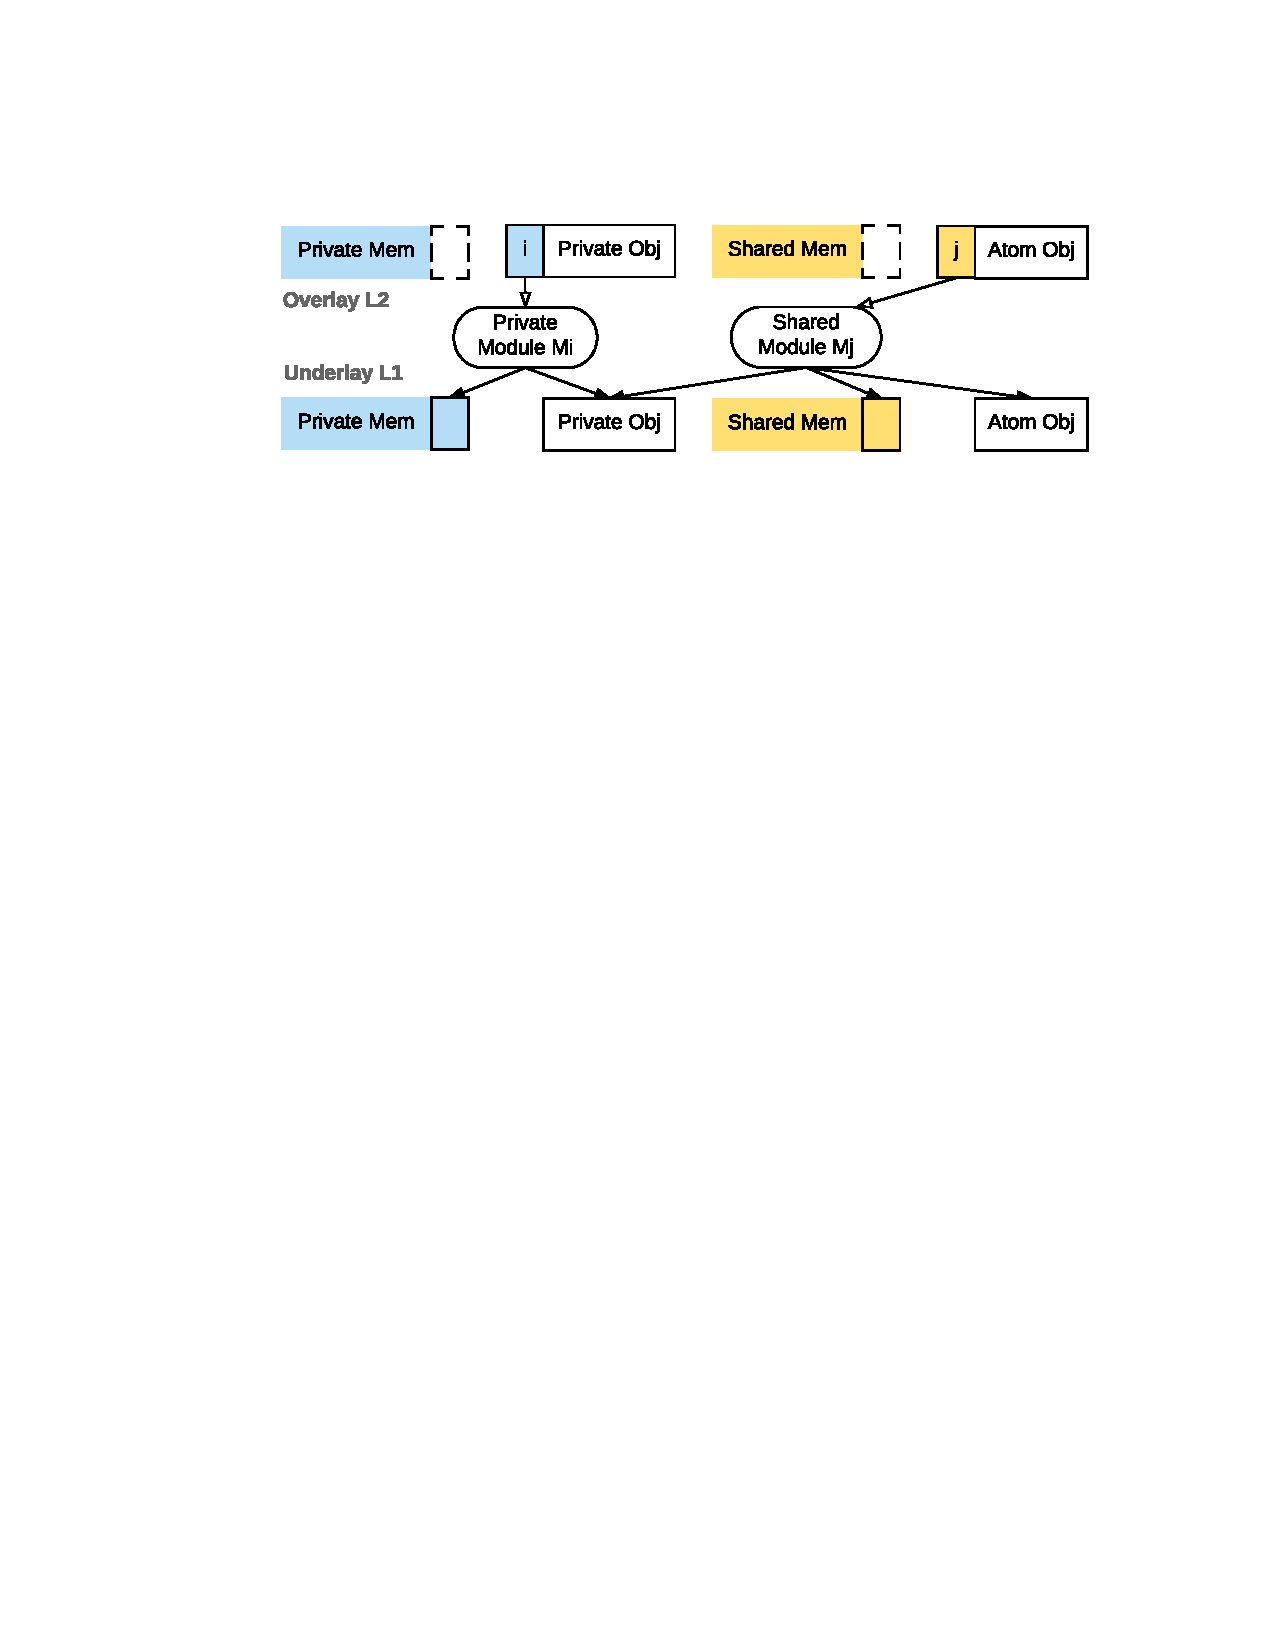
\includegraphics[scale=0.55]{figs/build_object}
\vspace*{-8pt}	
\end{center}
\caption{Defining concurrent abstraction layers.}
\label{fig:spec:object}
\vspace*{-10pt}
\end{figure}


In this section, we explain the general layer design principles and present
how we use environment context to convert a concurrent layer into 
 CPU-local layers.
\ignore{that is suitable for reasoning about concurrent code in a CPU-local way.}

\vspace*{-3pt}
\paragraph{Multicore hardware} allows
all the CPUs to access the same piece of memory
simultaneously.
In {\CTOS}, we \emph{logically} distinguish the \emph{private memory} 
(\ie, private to a CPU or a thread) from the \emph{shared memory} 
(\ie, can be accessed by multiple CPUs or threads). 
The private memory does not
need to be synchronized, whereas non-atomic
shared memory accesses need to be protected by some synchronization mechanisms
(\eg, locks), which are normally implemented using atomic hardware instructions
(\eg, fetch-and-add). With proper protection,
each shared memory operation can be viewed as if it were atomic.

\vspace*{-3pt}
\paragraph{Atomic object}
\ignore{In {\CTOS}, we refine each piece of shared data with well synchronized operations
into an \emph{atomic object}. An atomic object}

is an abstraction of well-synchronized shared memory, combined
with operations that can be performed over that shared memory.
It consists of a set of
primitives, an initial state, and a \emph{logical log} containing the entire
history of the operations that were performed on the object during
an execution. Every primitive invocation
records a \emph{single} corresponding event in the log. 
We require that these events contain enough information to derive the
current state of an atomic object by replaying the entire log starting 
from the object's initial state.
\ignore{ 
Note that every atomic primitive at the overlay always generates
exactly one event (this is how we make sure that it is really atomic),
while the actual implementation may trigger multiple events (by
calling multiple atomic primitives at underlay). The events are are
shuffled and merged during the contextual refinement, which we explain
in more detail in the subsequent subsections.
}

\vspace*{-3pt}
\paragraph{Concurrent layer interface}
$L$ is a collection of both \emph{private objects} and \emph{atomic objects},
along with some invariants imposed on these objects.
The verification of a concurrent kernel 
requires repeatedly 
building certified abstraction layers $(L_1, M, L_2)$.
The overlay interface $L_2$ is a
new and more abstract interface
built upon the underlay interface $L_1$ using module $M$
 (\cf Fig.~\ref{fig:spec:object}).
\emph{Private objects} are built from private modules with 
only private memory accesses
using techniques similar to those presented by Gu {\it et al} \cite{dscal15}. 
\emph{Atomic objects} are built from the 
existing atomic objects, private objects,
and modules with non-atomic shared memory accesses.

\ignore{
The framework requires the defined invariants to hold at any point in
the program execution. Invariant proofs are found to be particularly
challenging even in the sequential setting, where in many cases,
some invariants are temporarily violated and re-established later \cite{klein2009sel4}.
In {\CTOS}, thanks to our layered approach, we can impose different invariants
at different abstraction layers. The primitives at underlay can be hidden if they
are no longer needed at overlay, such that stronger invariants can be introduced
at some overlay with atomic primitives, which could otherwise be violated by the
lower-level primitives at underlays.
}

\ignore{
\paragraph{Verification task}
The major task to verify a concurrent kernel
is to show that kernel modules with shared memory accesses
have atomic interfaces.
In other words, the verification of a concurrent kernel
is a procedure to 
build new atomic objects based on the 
existing atomic objects, private object,
and non-atomic shared data
(\cf Fig.~\ref{fig:spec:object}).}
 
\vspace*{-3pt}
\paragraph{Verification task}
It is difficult to build certified abstraction layers
directly on
a multicore, nondeterministic hardware model. To build an atomic object,
one must reason about all of the unnecessary interleavings (\eg, the interleavings
between private operations), and prove that every access to shared memory is
well synchronized. Furthermore, it is not clear how we can reason about threads
running on each core locally and combine the proofs to obtain a global claim about the whole system.

In the remainder of this section, we first present our x86 multicore machine model
($\mach{x86mc}$), and then show how we gradually refine this low-level model into a
more abstract machine model ($\mach{loc}$) that is suitable
for reasoning about concurrent code in a CPU-local fashion.

\begin{figure*}
\begin{center}
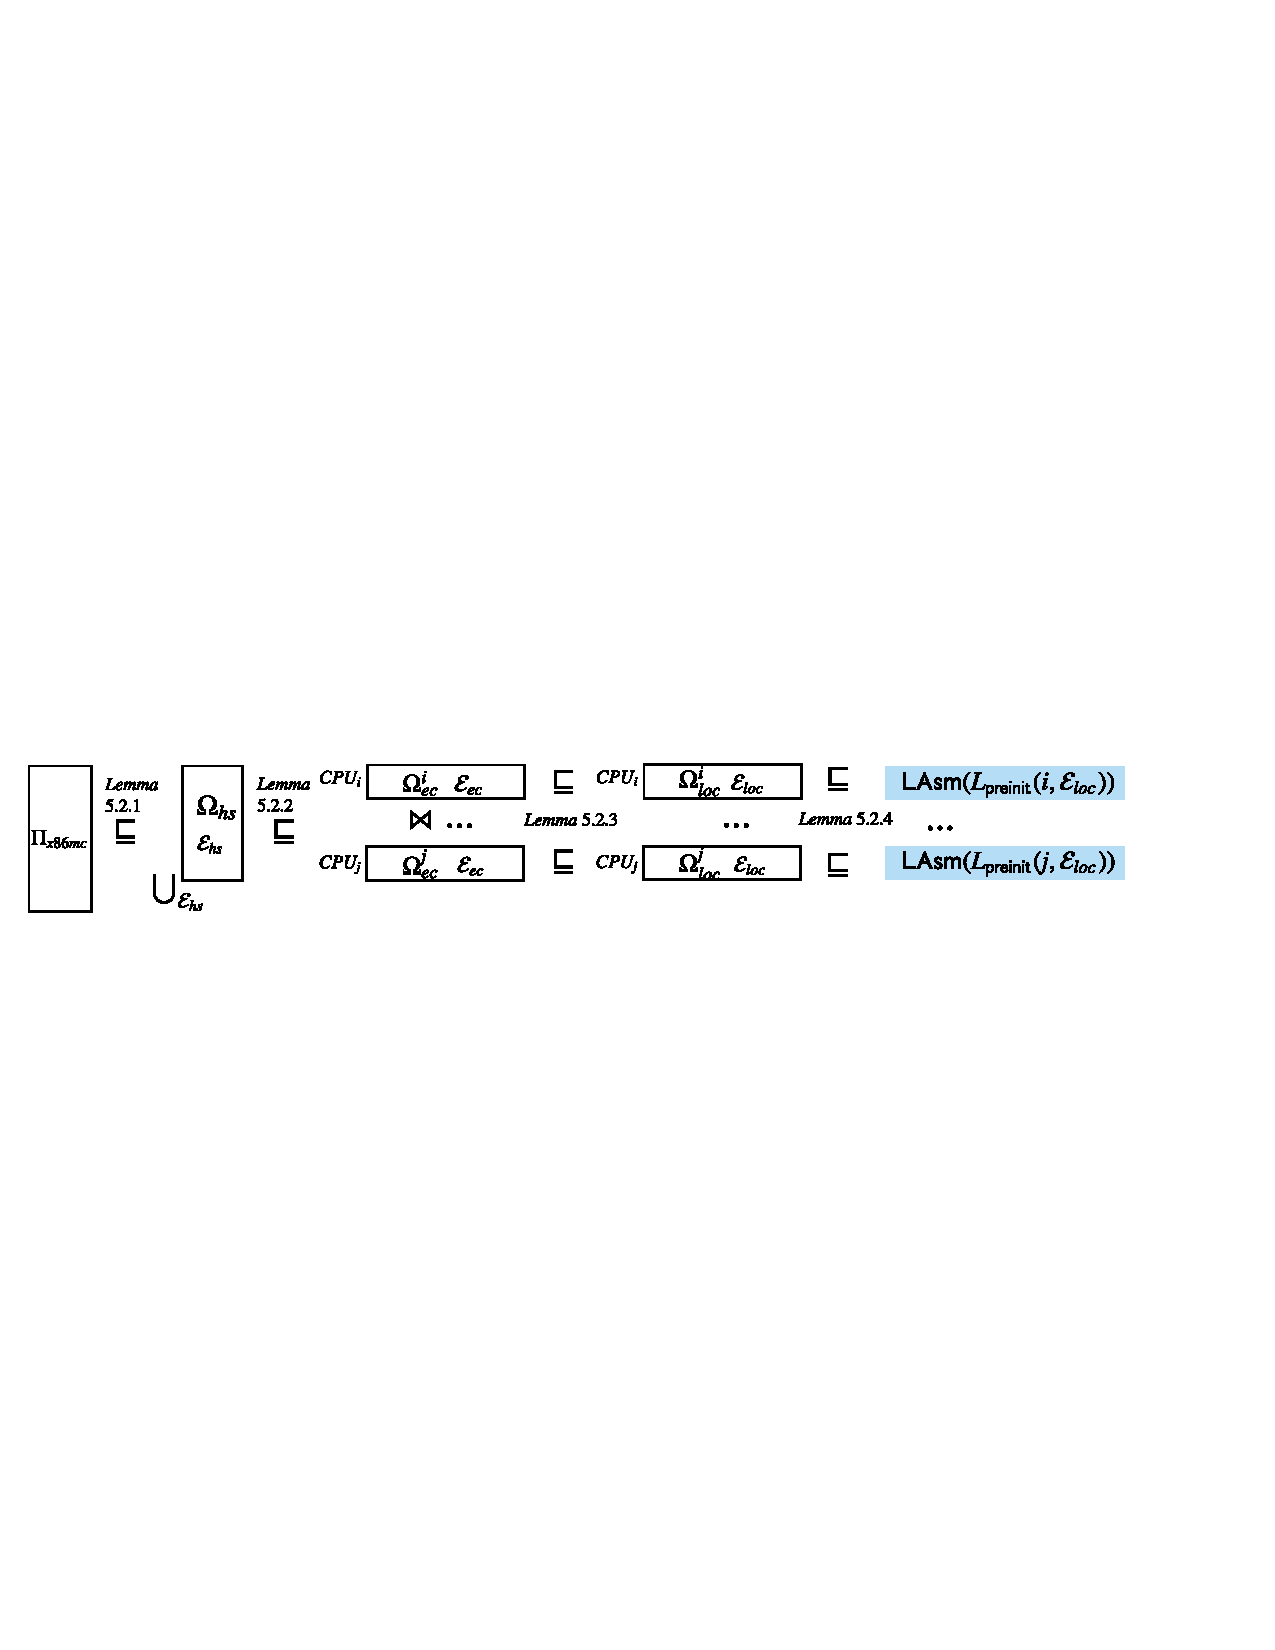
\includegraphics[scale=0.8]{figs/machine_chain}
\vspace*{-8pt}	
\end{center}
\caption{The contextual refinement chain from multicore hardware model
$\mach{x86mc}$ to CPU-local model $\mach{loc}$.}
\label{fig:spec:chain}
\vspace*{-10pt}
\end{figure*}

\vspace*{-2pt}
\subsection{Multicore hardware model}
Our fine-grained multicore hardware model ($\mach{x86mc}$) allows arbitrary
interleavings at the level of \emph{assembly instructions}.
At each step, the hardware \emph{randomly} chooses one CPU 
and executes the next assembly instruction on that CPU.
Each assembly instruction is classified as \emph{atomic}, \emph{shared},
or \emph{private}, based on if it involves an atomic object call,
a  non-atomic shared memory access, or only a private 
object/memory access.
One interleaving of an example program running on two CPUs
is:\vspace{-5pt}
\[
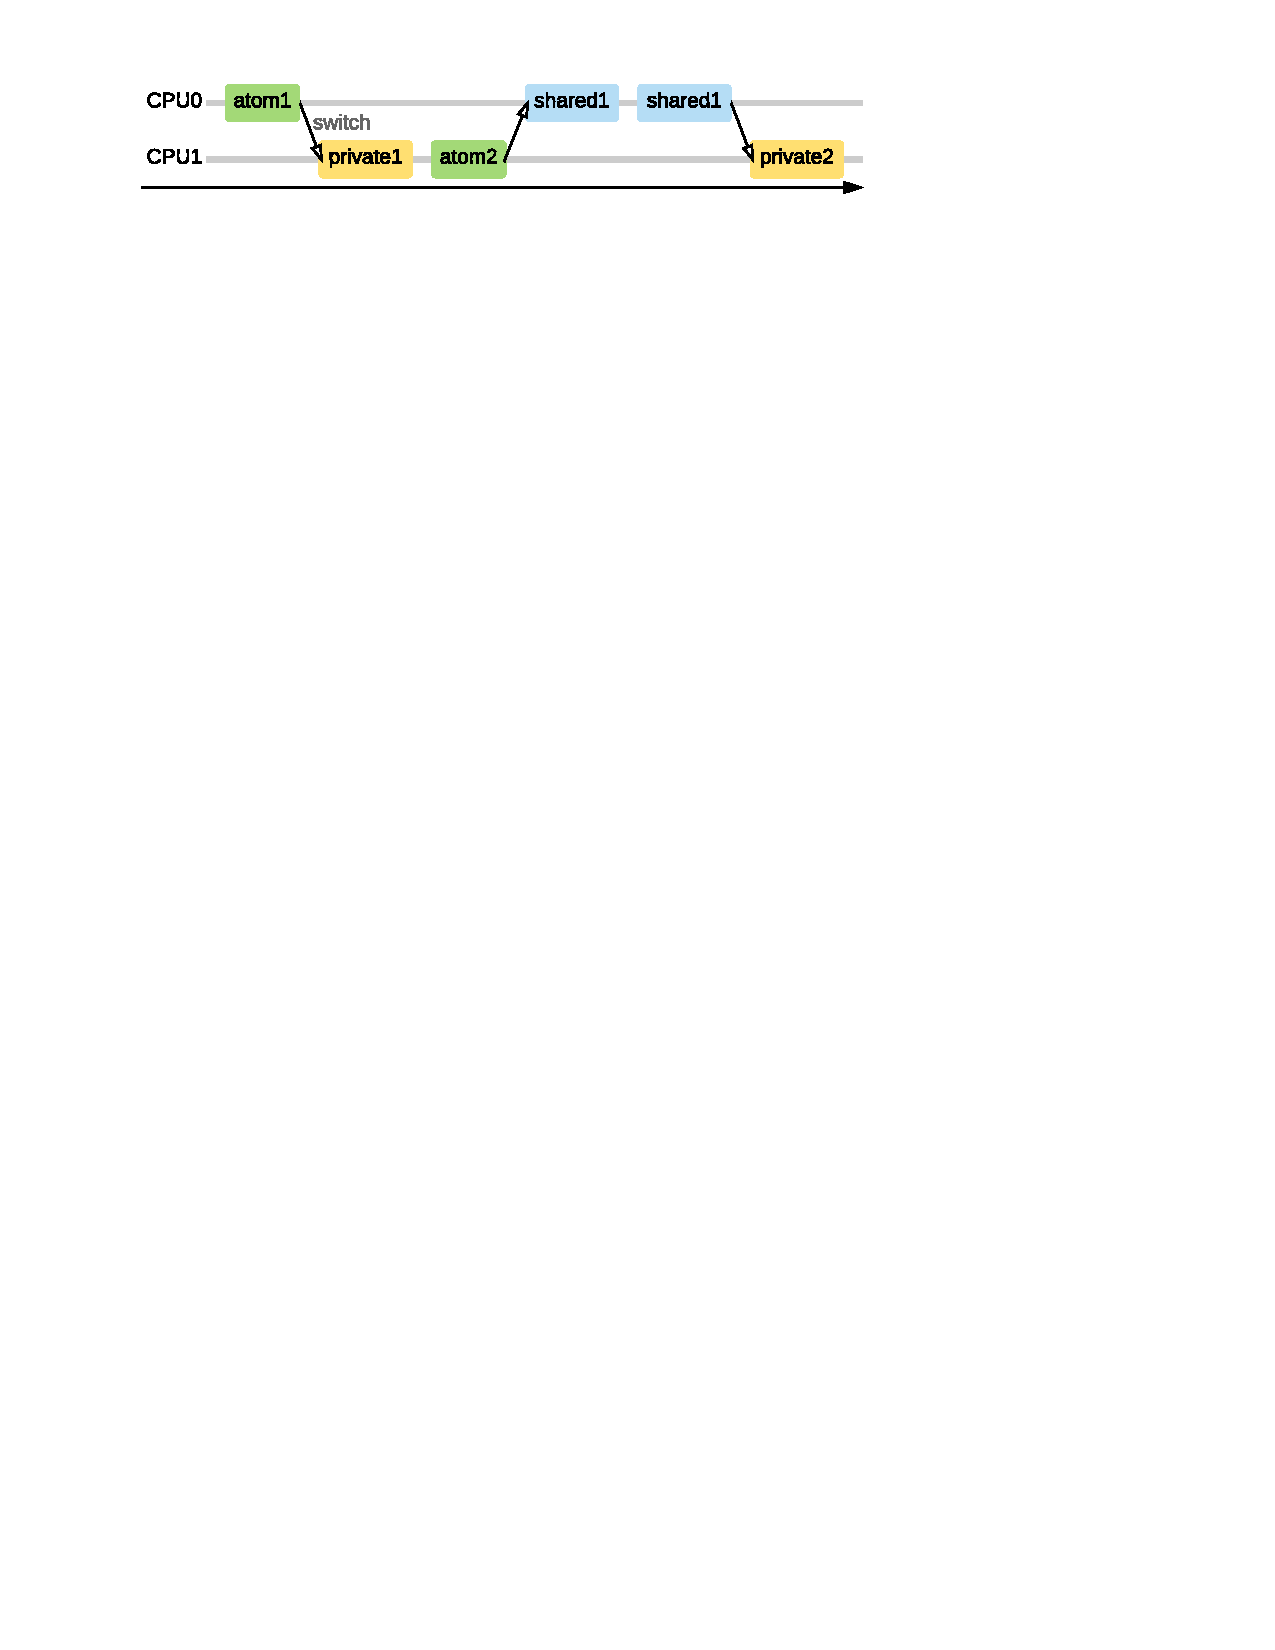
\includegraphics[scale=.65]{figs/machine1}
\vspace{-5pt}
\]
Since only atomic operations generate events,
this interleaving produces the logical log $[\event{0.atom_1,1.atom_2}]$.
\ignore{
Note that, while we mentioned above that each atomic object has its own
logical log, our model will actually maintain only a single log throughout an
execution. To obtain a per-object log, one can simply ignore all events in the
log that do not pertain to the desired atomic object.}

\ignore{
\paragraph{Memory model}
\ignore{
\ronghui{Maybe we do not need to talk about Compcert memory model?}
Because we use CompcertX~\cite{dscal15} along with
its formalization of the semantics of C and assembly,
our notion of memory is based on the CompCert memory model~\cite{leroy08}.
CompCert employs a unified model
to encode different views of memory.
The memory is split into a number of disjoint blocks and
a pointer is represented by a pair $(b, o)$, where
$b$ is a block identifier and
$o$ is an offset within block $b$.
Each offset within a block is associated with a permission
specifying the memory operations that can be performed at that location.
A program which attempts to perform a prohibited operation will \emph{get stuck}.
}

We \emph{logically} divide the machine memory into three parts:
\emph{atomic object}, \emph{shared memory},
and \emph{private memory}.
An \textbf{atomic object}
is accessed only through atomic operations
(\eg, compare-and-swap) provided by the hardware. Since these atomic operations
(denoted as \code{atom\_op})
are expensive, they are only used to implement the synchronization mechanisms
(\eg, locks). In our hardware model, each atomic operation generates 
\emph{exactly one event} that is recorded in a 
list of atomic events called a \emph{logical log}.
As shown in the ticket lock example \ronghui{reference?},
both \emph{ticket} and \emph{now} fields belong to the atomic object
and their operations generate the events $\event{inc\_ticket}$
and $\event{get\_now}$. Each method on the atomic object is considered
as atomic (as specified in the hardware manual) and its interface
is represented as a single
event. The values of an atomic object can be reconstructed from its logical log. 
\newman{I assume the events, log, and replay functions will be defined somewhere
in the Overview section?}

Operations to access shared memory and private memory
are denoted as \code{shared\_op} and \code{private\_op}, respectively.
Distinguishing between these makes it easier to reason about CPU-local 
execution.


\paragraph{Building atomic objects}
Shared memory accesses are not atomic. 
To ensure safety of the kernel,
shared memory has to be protected by synchronization
methods implemented using atomic objects.
The main task when verifying shared modules is to show that
each operation over shared memory can be viewed as if it were
atomic, provided the access is well synchronized by the atomic objects.
Therefore, concurrent kernel verification can be viewed as a procedure
to build concurrent objects with atomic interfaces (\cf Sec.~\ref{subsec:layer_def}).

\paragraph{Interleaving semantics}
}

\vspace*{-2pt}
\subsection{Machine model with hardware scheduler}
As a first step toward abstracting away the low-level details of
concurrent CPUs, we introduce a new machine model ($\mach{hs}$) configured
with a
\emph{hardware scheduler} ($\hardoracle$) that specifies a 
particular interleaving for an execution. 
This results in a deterministic machine model.
To take a program from $\mach{x86mc}$ and run it on top of $\mach{hs}$,
we insert a  \emph{logical \intptext}
(denoted as ``$\intp$") before each assembly instruction.
At each \intptext, the machine first queries the hardware scheduler
and gets the CPU ID to execute next.
All the \emph{switch decisions} made by $\hardoracle$ are stored in the 
log as switch events. 
The previous example on $\mach{x86mc}$
can be simulated by the following $\hardoracle$:\vspace{-5pt}
\[
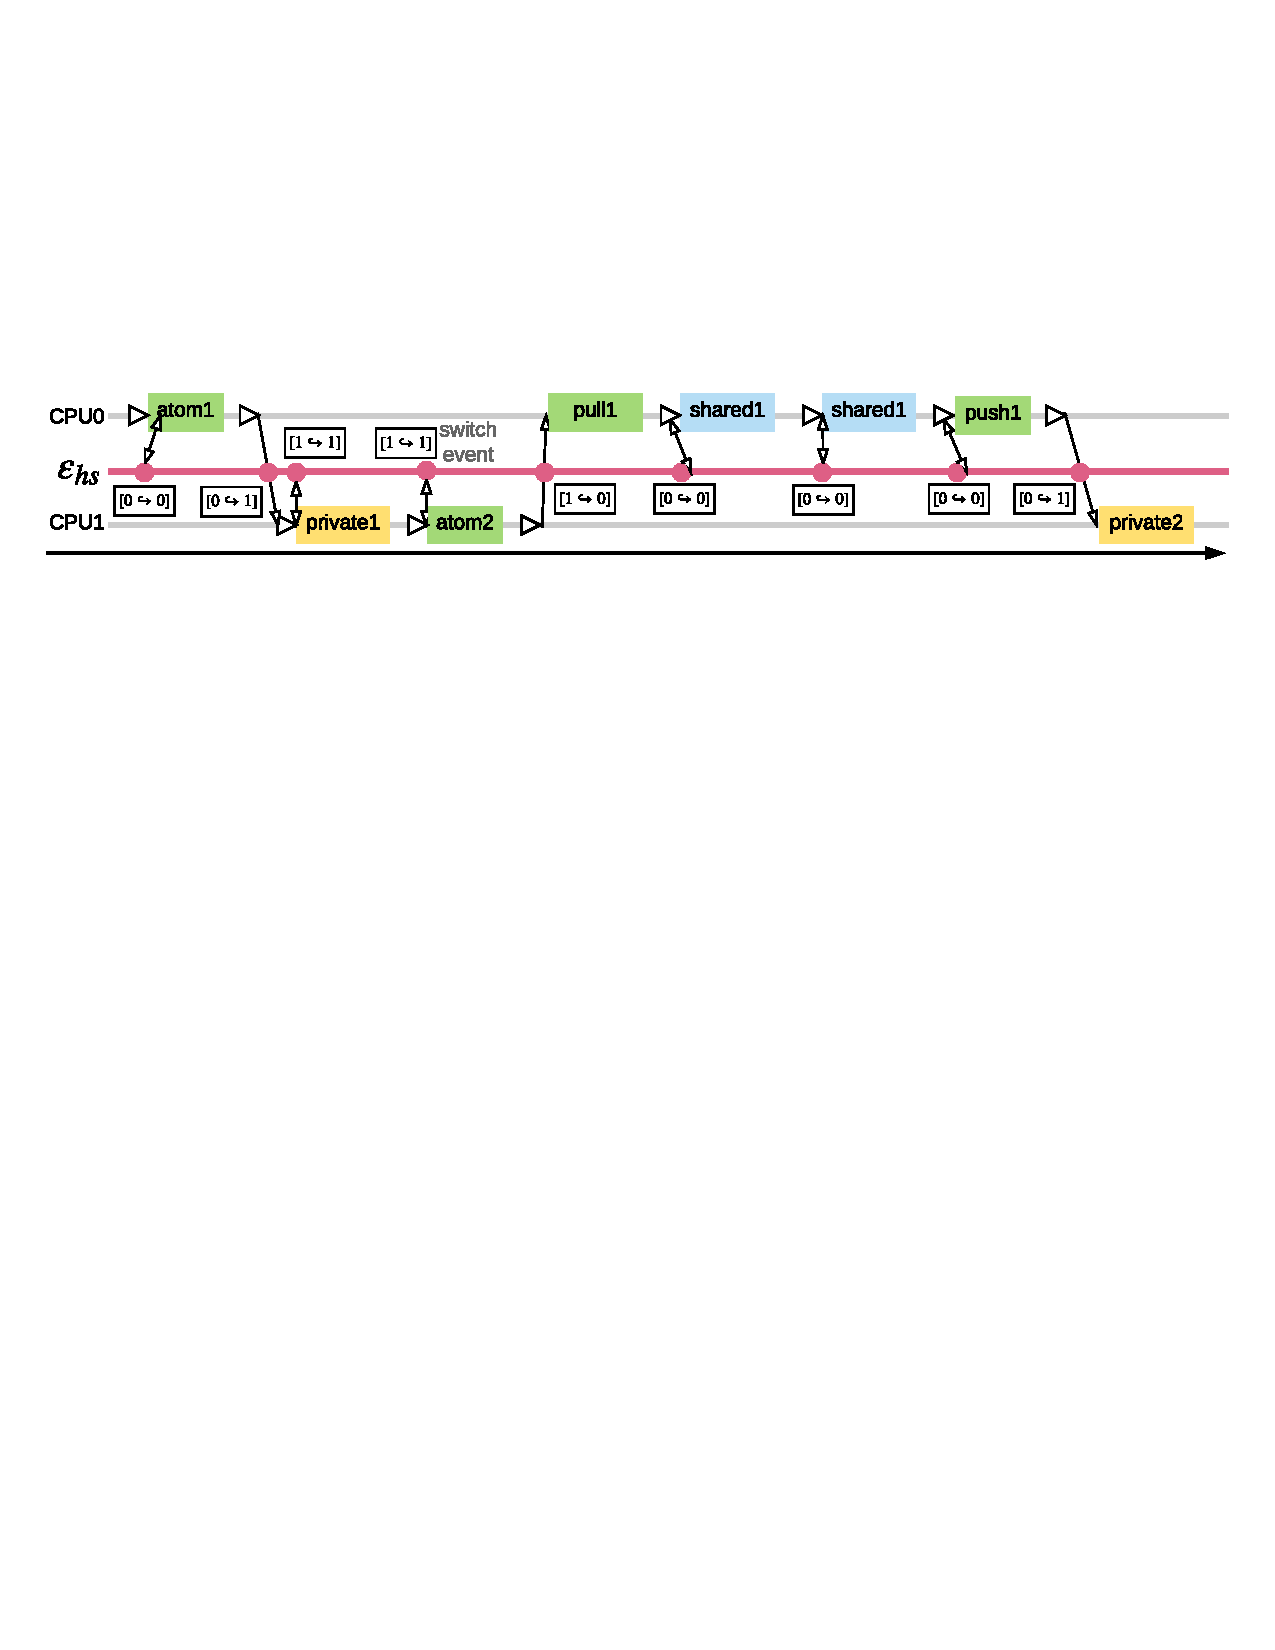
\includegraphics[scale=.52]{figs/machine2}
\vspace{-5pt}
\]

\noindent
The log recorded by this execution is as follows
(a switch from CPU $i$ to $j$ is denoted as $i\switch j$):\vspace{-5pt}
%%%
\[
\begin{footnotesize}
\begin{array}{l}
\!\!\!\!\![\event{0\switch 0, 0.atom_1,  0\switch 1, 1\switch 1,}
\event{1\switch 1, 1.atom_2, 1\switch 0, 0\switch 0,  0\switch 1}]
\end{array}
\end{footnotesize}
\vspace{-5pt}
\]

The behavior of running a program $P$
over this model with a hardware scheduler $\hardoracle$
is denoted as $\mach{hs}(P,\hardoracle)$.
Let $\ectxtc_{hs}$ represents the set of all possible hardware
schedulers. Then we define the whole-machine semantics.
{\small \[
\sem{hs}{P} = \{ ~ \mach{hs}(P,\hardoracle) ~ \mid ~ \hardoracle \in \ectxtc_{hs} ~ \}
\vspace{-15pt}
\]}

\ignore{The machine model with hardware scheduler is denoted as $(\mach{hs}, \hardoracle)$,
to indicate that it is parametrized over all possible $\hardoracle$.}

\noindent
Note that this is a special case of the definition in Sec.~\ref{sec:overview}
for the whole-machine semantics of a concurrent layer machine, where the 
active set is the set of all CPUs.
To ensure correctness of this machine model with respect to the hardware machine model,
we prove that $\mach{x86mc}$ \emph{contextually refines} the new model.
Before we state the property, we first define the notion of
\emph{contextual refinement} formally.

\begin{definition}[Contextual Refinement]
\label{def:mach:refine}
We say layer $L_0$ 
\emph{contextually refines}
layer $L_1$ (written $\forall P, \sem{L_0}{P}\machrel \sem{L_1}{P}$),
iff, for any $P$ that 
does not go wrong 
on $\machx_{L_1}$ under any configuration, (1)~$P$ does not go wrong on $\machx_{L_0}$
under any configuration;
and (2)~any observable behavior of $P$ on $\machx_{L_0}$
under some configuration is also observed on $\machx_{L_1}$
under some (possibly different) configuration.
\end{definition}

\begin{lemma}[Correctness of the hardware scheduler model]\vspace{-3pt}
\label{lemma:hs}
\begin{small}
$$\forall P, \sem{x86mc}{P}\machrel \sem{hs}{P}$$
\end{small}
\vspace{-10px}
\proof[Proof Sketch]
For any interleaved execution on $\machx_{x86mc}$, we construct
a corresponding hardware scheduler on $\mach{hs}$.

\ignore{
Given an observable execution behavior of $P$ running on
$\machx_{x86mc}$, we can construct a particular hardware scheduler
$\hardoracle$ encoding the interleaving that produced the behavior.
The resulting behavior $\mach{hs}(P,\hardoracle)$ is then
an element of $\sem{hs}{P}$ by definition.
}

\ignore{\proof
For any $P$ and any possible interleaving on $\mach{hw}$,
there exists a corresponding hardware scheduler $\hardoracle$,
such that $P$ exhibits an equivalent
behavior when it runs on top of $(\mach{hs}, \hardoracle)$.
\qed}
\end{lemma}

\ignore{
Lemma \ref{lemma:hs} ensures that for
any program running on top of the machine $\mach{hw}$, there exists
a hardware scheduler such that the program exhibits an equivalent
behavior when it runs on top of $\mach{hs}$ with the
hardware scheduler.}

\vspace{-5pt}
\subsection{Machine with local copy of shared memory}
The above machine model does not restrict any access to the shared memory.
We therefore abstract the machine model with hardware scheduler into
a new model that enforces well-synchronized accesses to shared memory.

In addition to the global shared memory concurrently manipulated by all CPUs,
each CPU on this new machine model ($\mach{lcm}$) also maintains
a local copy along with a \emph{valid bit}.
The relation between a CPU's local copy and the global shared memory
is maintained through two new \emph{logical} primitives $\code{pull}$ and $\code{push}$.
The $\code{pull}$ operation updates a CPU's local copy to be equal to the shared memory,
marking the local copy as $\code{valid}$ and the shared memory as $\code{invalid}$.
Conversely, the $\code{push}$ operation updates the shared memory
to be equal to the local copy, marking the shared memory
as $\code{valid}$ and the local copy as $\code{invalid}$.
If a program attempts to pull an $\code{invalid}$ shared memory, push
an $\code{invalid}$ local copy, or access an $\code{invalid}$ local copy,
the program goes wrong.
It makes sure that every shared memory access is always performed on
its $\code{valid}$ local copy, thus systematically enforcing valid accesses to the
shared memory.
Note that all of these constructions are completely \emph{logical}, and do not
correspond to any physical protection mechanisms; thus they do not introduce any
performance overhead.

The shared memory updates of the previous example can be simulated 
on $\mach{lcm}$ as follows:\vspace{-5pt}
\[
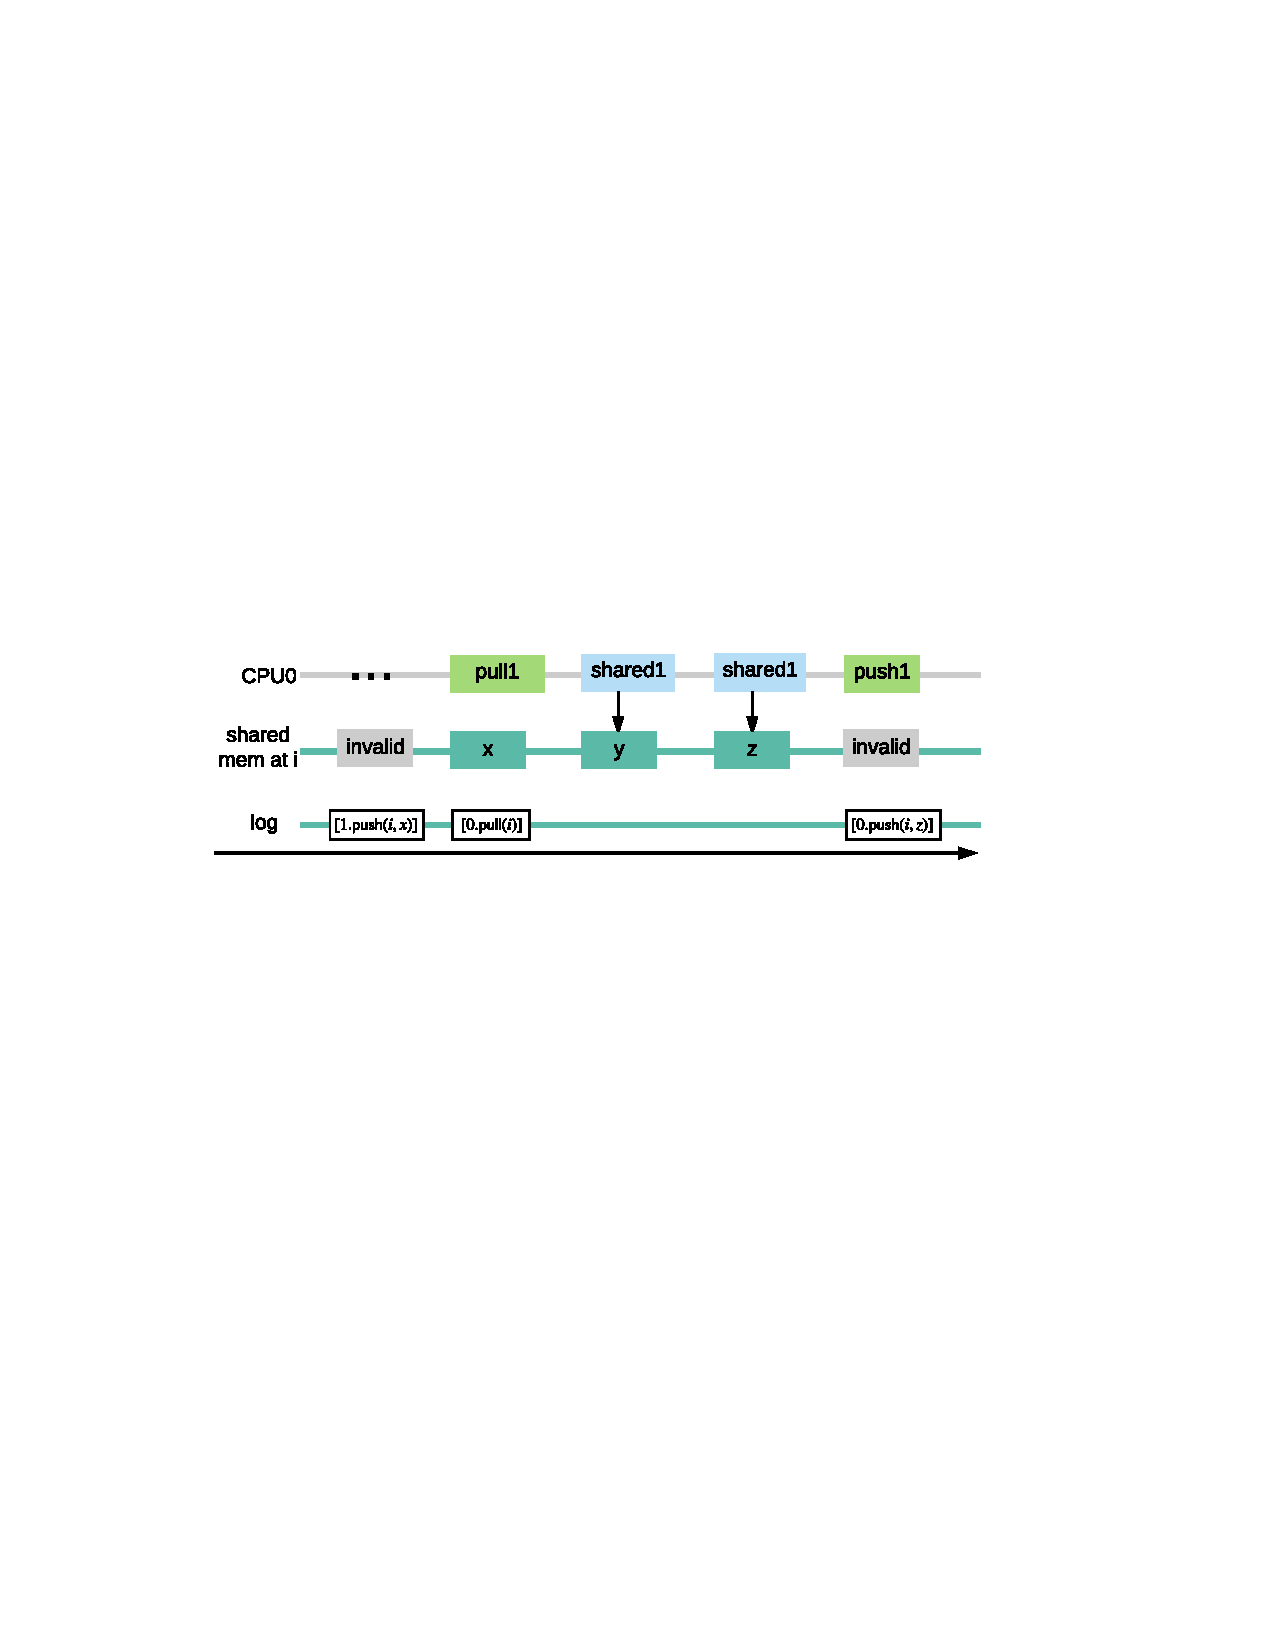
\includegraphics[scale=.6]{figs/machine3}
\vspace{-5pt}
\]

\paragraph{Data-race freedom}
Among the global shared memory and all the local copies, only one can be $\code{valid}$ at any single moment of 
machine execution. 
Therefore, for any program $P$ with a potential \emph{data race}, there exists
a hardware scheduler such that $P$ goes wrong on $\mach{lcm}$.
By showing that a program $P$ is safe (never goes wrong) on $\mach{lcm}$
for \emph{all possible} hardware schedulers, we guarantee that $P$ is data-race free. 

It remains to show that $\mach{lcm}$ is correct with
respect to the previous machine model $\mach{hs}$
with the $\ectxtc_{hs}$.
\begin{lemma}[Correctness of the local copy model]\vspace{-2pt}
{\small \[
\forall P, \sem{hs}{P}\machrel \sem{lcm}{P}\]}
\vspace{-20pt}
%%%
\ignore{
\[\forall \hardoracle, (\mach{hs}, \hardoracle) \machrel 
(\mach{lcm},\hardoracle)\]
}
\ignore{\[\forall P\ \hardoracle, \machbe{P}{\mach{hs}}{\hardoracle}\machrel 
\machbe{P}{\mach{lcm}}{\hardoracle}\]
\proof
For any possible $\hardoracle$, if the program $P$ is safe on $\mach{lcm}$,
then the observable behavior of $P$ on $\mach{lcm}$ is equivalent to
the behavior of $P$ running over $\mach{hs}$.
\qed}
\end{lemma}

\subsection{Partial machine with environment context}

Although $\mach{lcm}$ provides a way to reason about shared memory operations,
it still does not have much support for CPU-local reasoning.
To support modular verification, the machine model should provide
a way to reason about programs on each CPU locally by specifying
expected behaviors of the context programs on other CPUs. The model
should then provide a systematic
way to link the proofs of different local components together to form a global
claim about the whole system. To this purpose, we introduce a partial
machine model $\mach{pt}$ that can be used to reason about the
programs running on a subset of CPUs, by
parametrizing the model over the behaviors of an \emph{environment context}
(\ie, the rest of the CPUs).

We call a given local subset of CPUs the \emph{active CPU set} 
(denoted as $A$).
\ignore{, while all other CPUs are called the 
\emph{context CPU set}.
 of $A$
(denoted as $\overline A$).}
The partial machine model is configured with an active CPU set,
and it queries the environment context whenever it reaches a switch point
that attempts to switch to a CPU outside the active set.

\vspace{-2pt}
\paragraph{Environment context}
of $A$ in this machine model 
is denoted as $\ectxt{pt,A}$.
Each environment context $\oracle_{pt(A)}\in\ectxt{pt,A}$
is a \emph{response function},
which takes the current log 
and returns a list of events from the context programs (\ie, those outside of $A$) 
that is guaranteed to satisfy some invariant.
In other words, response function simulates the observable behavior 
of the context CPUs, and the invariant states the assumptions being 
made over the context.
The hardware scheduler
is also a part of the environment context,
\ie, the events returned by the response function include
switch events. The execution of CPU 0 in the previous example can be simulated
with a $\oracle_{pt(\set{0})}$.
\ignore{$\oracle_{\overline{\set{0}}}$
(\ie, $\oracle_{\set{1}}$, since there are only two CPUs).}\vspace{-2pt}
\[
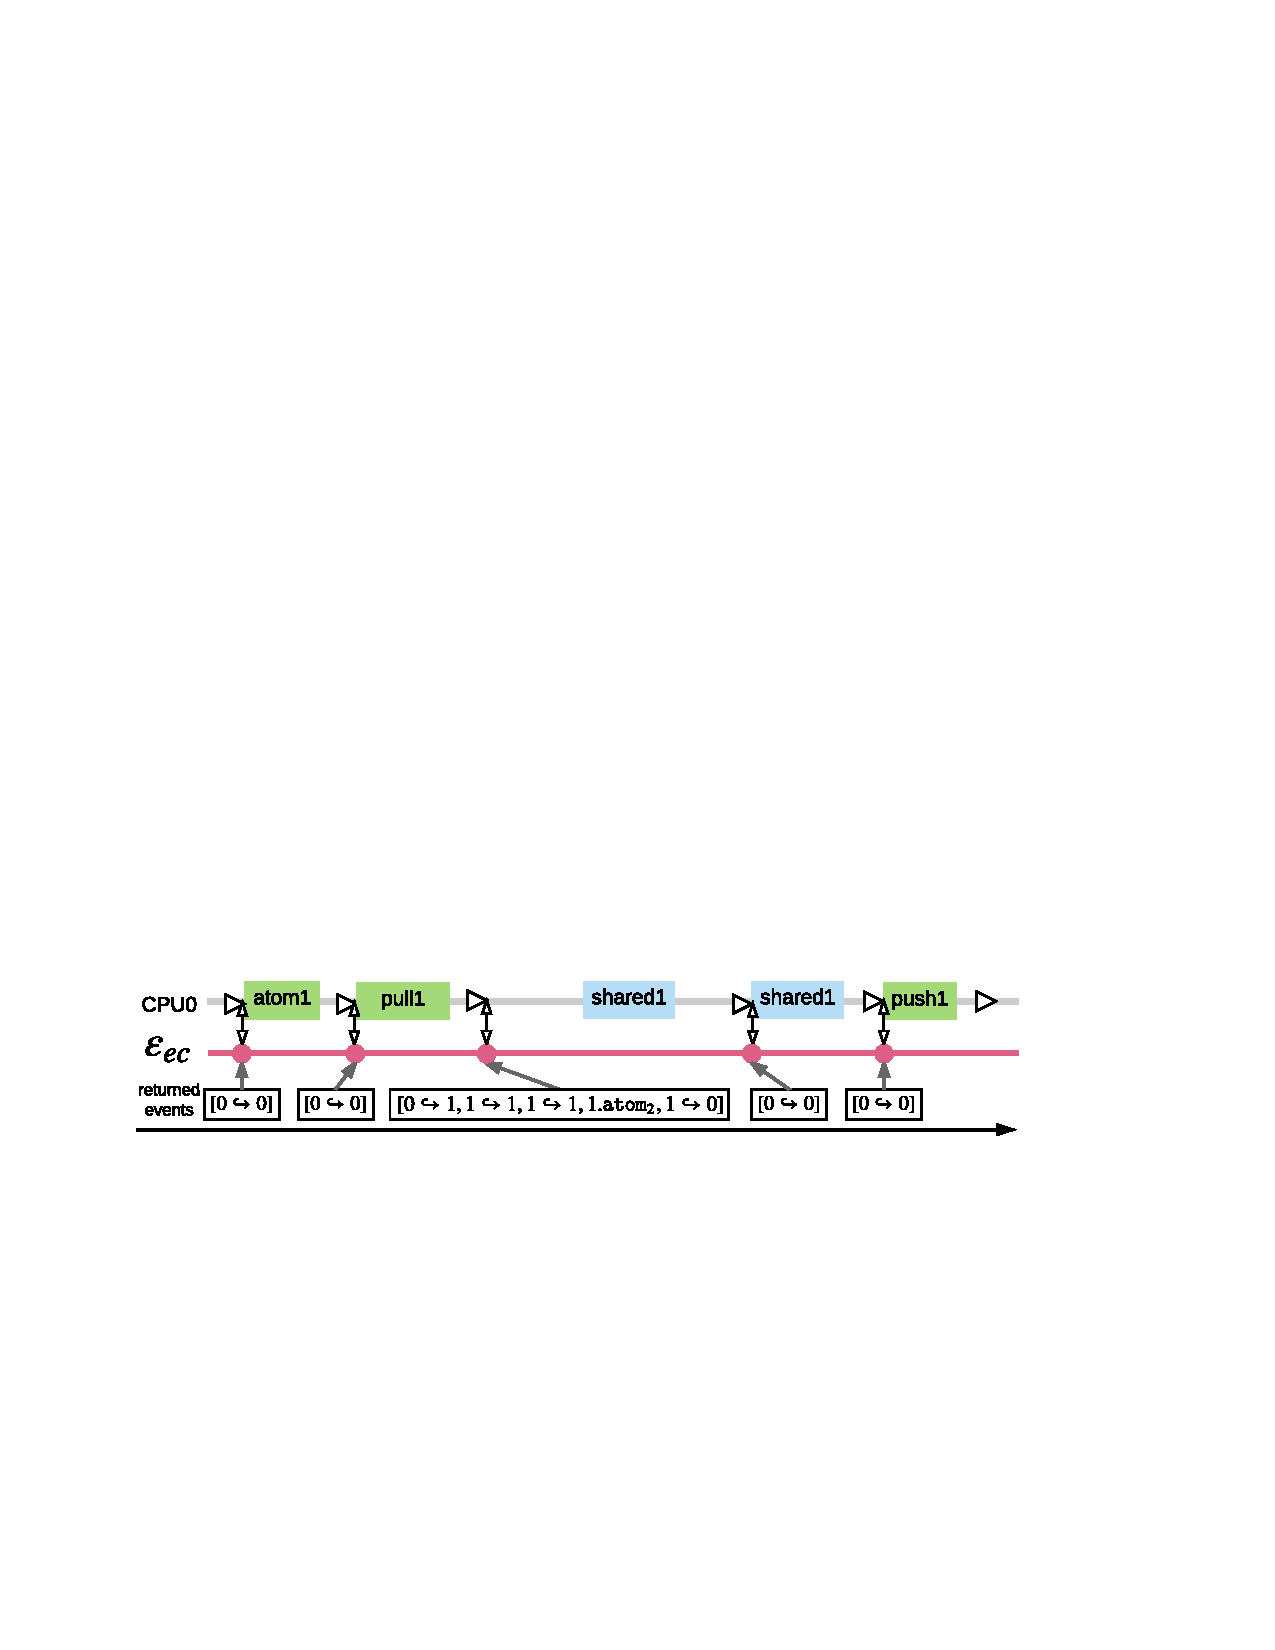
\includegraphics[scale=.53]{figs/machine4}
\vspace{-3pt}
\]

\ignore{The environment context $\oracle_{\set{1}}$
generates the event list $[\event{0\switch 1},\event{1\switch 1},\event{1\switch 1}, \event{1.atom_2}, \event{1\switch 0}]$
at the third \intptext.}

\paragraph{Composition of partial machine models}
Suppose we have verified that two programs, separately running with two 
\emph{disjoint} active CPU sets $A$ and $B$, produce event lists
satisfying invariants $\inv_A$ and $\inv_B$, respectively.
If $\inv_A$ is consistent with the environment context invariant
of $B$,\ignore{(\ie,  $\ectxt{pt,B}$)\ronghui{Do we need this i.e. ?},}
and $\inv_B$ is consistent with the environment context invariant of 
$A$,\ignore{ (\ie, $\ectxt{pt,A}$),}
then we can compose the two separate programs into a single program
with active set $A \cup B$.
This combined program is guaranteed to produce event lists
satisfying the combined invariant $\inv_A \wedge \inv_B$.
Formally, using the whole-machine semantics definition from
Sec.~\ref{sec:overview}, we express this composition as a contextual 
refinement.

\begin{lemma}[Composition of partial machine models]\vspace{-2pt}
\label{lemma:compose}
{\small \[\forall P, \sem{pt(A\cup B)}{P}\machrel \sem{pt(A)}{P} \cap \sem{pt(B)}{P}\quad \text{if } A \cap B = \emptyset\]}
\vspace{-17pt}
\ignore{
\[
\begin{array}{l}
\forall \oracle_{A}\  \oracle_{B}\
\oracle_{\overline{A\cup B}},\\
(\mach{pt},
\oracle_{\overline{A\cup B}})_{A\cup B}
= (\mach{pt},
\oracle_B
\cup \oracle_{\overline{A\cup B}})_A \bigcap
(\mach{pt},
\oracle_A \cup \oracle_{\overline{A\cup B}})_B
\end{array}
\]
}
\ignore{
\proof
If the environment contexts of program $P$ running on $A$ and $B$ are consistent,
then it is equivalent to running $P$ on $A\cup B$ directly. 
\qed}
\end{lemma}

After composing the programs on all CPUs, the context CPU set becomes
empty, and the composed invariant holds on the whole machine.
Since there is no context CPU, the environment context is
reduced to the \emph{hardware scheduler}, which only generates the
switch events. In other words, letting $C$ be the entire set of CPUs
on the machine, we have that $\ectxt{pt,C} = \ectxtc_{hs}$.  By
showing that this \emph{composed machine} with the entire CPU set $C$
is refined by $\mach{lcm}$, the proofs can be propagated down to the
multicore hardware model.

\begin{lemma}[Correctness of the composed total machine]
{\small \[\vspace{-10pt}\forall P, \sem{lcm}{P}\machrel \sem{pt(C)}{P}\vspace{-10pt}\]}
\ignore{
\[
\forall \hardoracle,
(\mach{lcm}, \hardoracle)
\machrel 
(\mach{pt},\hardoracle)\]
}
\ignore{
\[
\forall P\ \hardoracle\ \inv,
\machbe{P}{\mach{lcm}}{\hardoracle}
\machrel 
\machbe{P}{\mach{pt}}{\hardoracle,\inv}\]
\proof
For any given $\hardoracle$, the only difference between two machine models is that
$\mach{partial}$ introduces the invariant $\inv$.
\qed
}
\end{lemma}

\subsection{CPU-local machine model}
\label{subsec:spec:seq}
If we focus on a single active CPU $i$,
the partial machine model is like a \emph{local} machine
with an environment context representing all other CPUs. However,
in this model there is a {\intptext} before each instruction,
so program verification still needs to handle many unnecessary 
interleavings (\eg, the ones between private operations).
In this subsection, we introduce a CPU-local
machine model (denoted as $\mach{loc}$) for a CPU $i$, in which {\intptext}s
only appear before atomic or $\code{push}$/$\code{pull}$ operations.
The {\intptext}s before shared or private operations
are removed via two steps: \emph{shuffling} and \emph{merging}.

\paragraph{Shuffling {\intptext}s}
In $\mach{loc}$, we introduce a \emph{log cache}~--- for
the {\intptext}s before shared and private operations,
the query results from the environment context
are stored in a temporary log cache.
The cached events are applied to the logical log
just before the next atomic or $\code{push}$/$\code{pull}$ operation.
Thus, when we perform shared or private operations,
the observations of the environment context are delayed
until the next atomic or $\code{push}$/$\code{pull}$ operation.
This is possible because a shared operation can only be performed
when the current local copy of shared memory is valid, meaning that 
no other context program can interfere with the operation.

\paragraph{Merging {\intptext}s} Once the {\intptext}s are shuffled properly,
we merge all the adjacent {\intptext}s together.
When we merge {\intptext}s, we also need to merge 
the switch events generated by the environment context.
For example, the change of {\intptext}s for the previous example
on CPU-local machine is as follows: 
\[
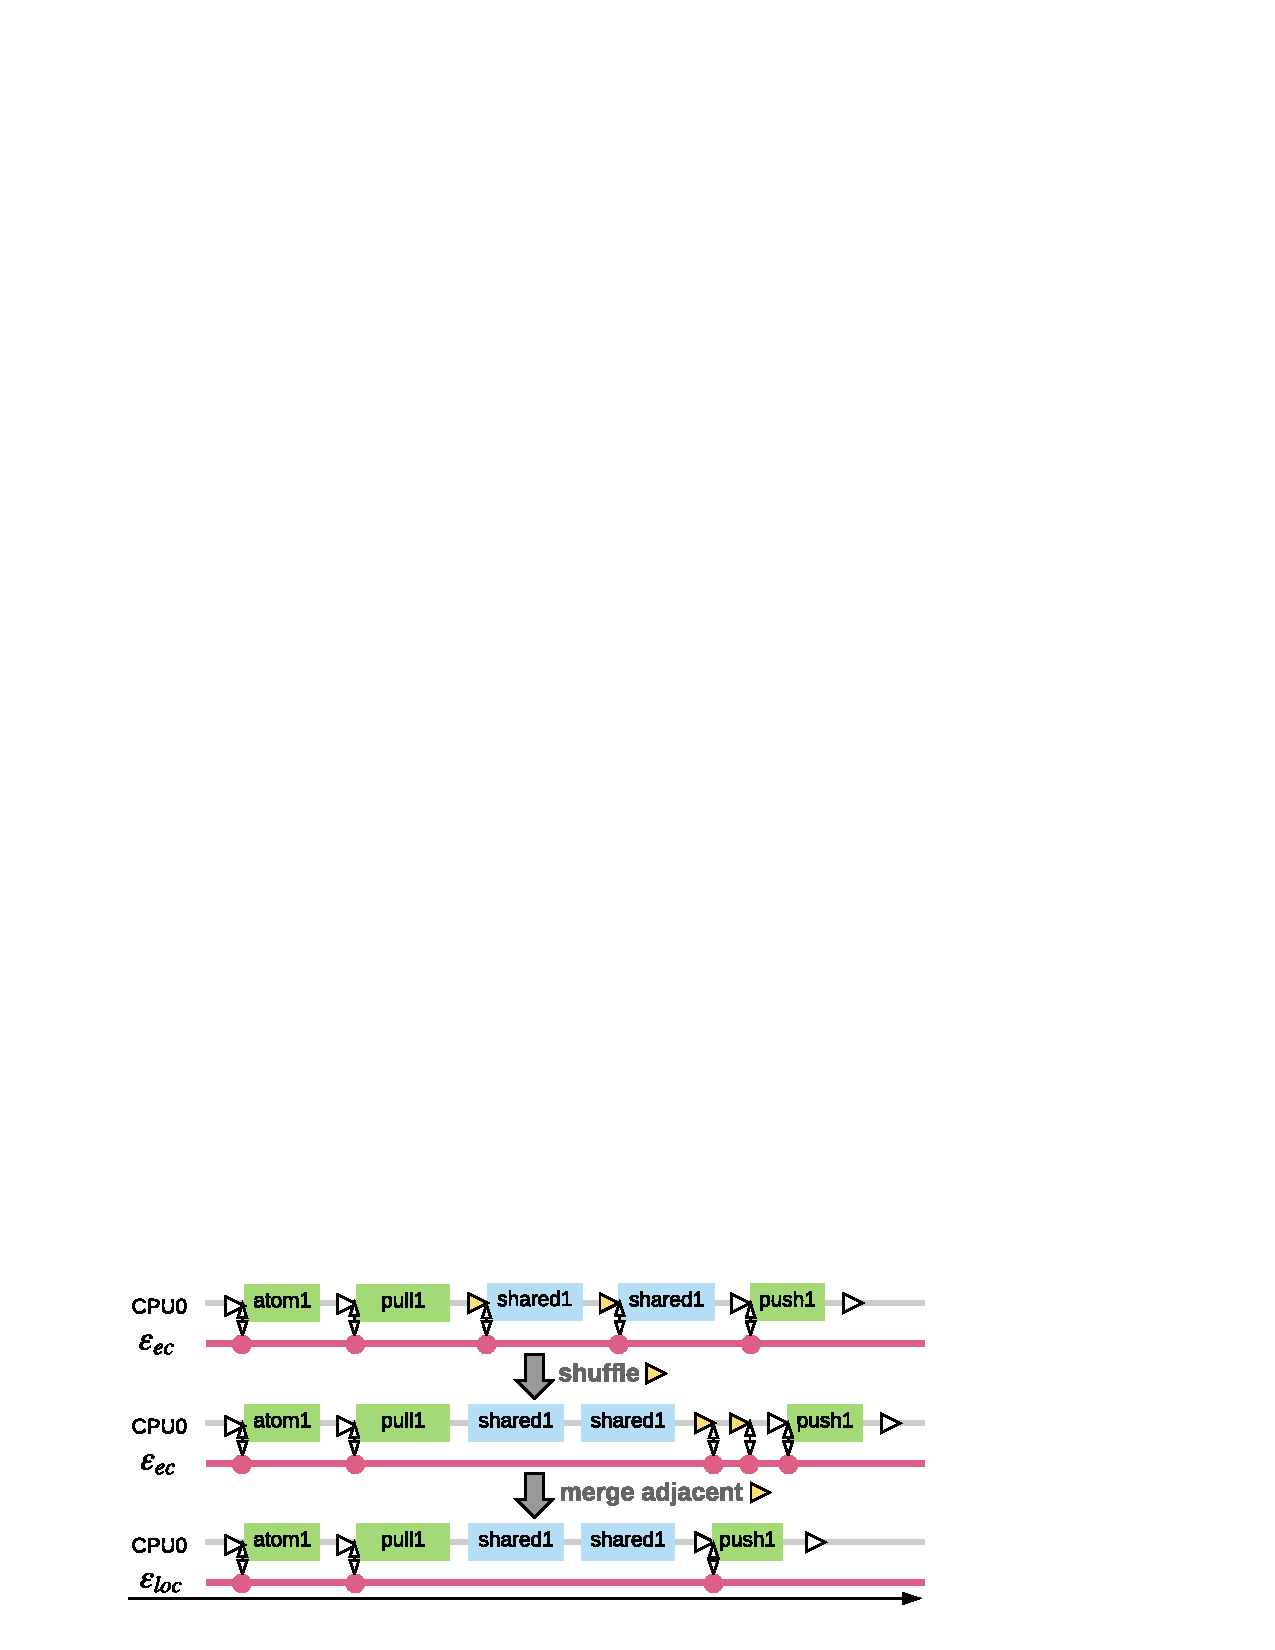
\includegraphics[scale=.57]{figs/machine5}
\]

\begin{lemma}[Correctness of CPU-local machine model]
{\small \[\forall P, \sem{pt(\set{i})}{P}\machrel \sem{loc(\set{i})}{P}\]}
\vspace{-23pt}

\ignore{
\[
\forall \oracle_{\overline{\set{i}}},
\exists \oracle'_{\overline{\set{i}}},
(\mach{pt},\oracle_{\overline{\set{i}}})_{\set{i}}
\machrel 
(\mach{loc},\oracle'_{\overline{\set{i}}})_{\set{i}}
\]
}
\ignore{\[
\begin{array}{l}
\forall P\ \oracle_{\overline{\set{i}}}\ \inv_{\set{i}},
\exists \oracle'_{\overline{\set{i}}},\\
\machbe{P}{\mach{pt}}{\oracle_{\overline{\set{i}}},  \inv_{\set{i}}}
\machrel 
\machbe{P}{\mach{loc}}{\oracle'_{\overline{\set{i}}}, \inv_{\set{i}}}
\end{array}
\]
\proof
Shuffling and merging {\intptext}s  are valid.
\qed}
\end{lemma}

Finally, we obtain the refinement relation from the multicore
hardware model
to the CPU-local machine model by composing
all of the refinement relations together (\cf Fig.~\ref{fig:spec:chain}).
We introduce and verify the {\mCTOS} kernel on top of the CPU-local machine
model $\mach{loc}$. The refinement proof guarantees that the proved properties can be
propagated down to the multicore hardware model $\mach{x86mc}$.





\ignore{
\newman{Copied from the overview section. I will merge them into this
section somehow.}
\subsection{Defining abstraction layers}

We define a concurrent
layer interface $L$ using three components: a collection of
\emph{private objects}, a collection of \emph{atomic objects}, and the
invariants which the atomic and private objects must satisfy at any
point of the execution.  These three components define a {\em logical}
view of a subset of the kernel code and extend an x86-like assembly
machine ($\machx$) with an abstract specification of that code. 

A {\em private object} is the abstraction of private date owned by a
particular thread (or process or CPU). It consists of an
\emph{abstract state} (serving as the abstraction of the underlying
private memory), and a collection of primitives (serving as the
specifications of the methods manipulating that piece of the private
memory). Fig.~\ref{fig:spec:object} shows how to build private
objects.

An {\em atomic object} is the abstraction of shared memory. All of
its methods/primitives are atomic.

As shown in Sec.XXX, the sequential machine model contains a
\emph{small} set of atomic objects, which generates a single event and
the object itself is constructable by replaying the logical log.

Figure~\ref{fig:spec:object} shows how to build atomic objects based
on the atomic objects, private objects, and the shared memory at
underlay.  Since the shared memory accesses are modeled using
\emph{local copy}, the \code{push/pull} operations have to be
synchronized using underlay's atomic objects.  The verification of
functions accessing shared data inside the kernel is a procedure to
show that all shared memory accesses are well-synchronized and its
invocation can be viewed as atomic.

For example, the physical page allocator scans the \emph{shared}
allocation table and returns the first free page.  Its accesses to the
shared table are protected by \emph{atomic lock objects}, such that
its \code{push/pull} operations are safe to execute.  By showing that
the allocator implementation satisfy the specification, which
generates a single \code{palloc} event, an atomic allocator object is
introduced and can be used to reason about other kernel modules at
higher layers (\cf Sec.\ref{sec:base:memm}).

We will use $\mach{L}$ to denote the resulting abstract machine for
each layer interface $L$





\paragraph{Layer invariant}
Each abstraction layer specifies a predicate
on the private objects' abstract states
and the logical log,
which is the invariant $\inv_{\set{i}}$ hold for the execution on CPU $i$
(\cf Sec.XXX).
We have to show that this invariant $\inv_{\set{i}}$ is preserved
by all primitives of private objects and atomic objects.
The proofs for atomic  objects also rely on the
invariant of the context CPUs (\ie, $\inv_{\bar{\set{i}}}$).

In previous verification efforts, even for private objects,
proving invariants has typically been challenging~\cite{klein2009sel4},
especially that the invariants might be temporarily violated within the function body.
For example, adding a new node to a doubly-linked list
temporarily violates invariants that the list is well formed.

However, in our layered approach,
we do not have to set up the all the invariants at a single step.
Take the thread queue (implemented as doubly-linked list) in C2 kernel as an example.
When verifying the concrete implementation, we do not pose the well-formedness invariant
over the queue at that layer.
We only prove the invariant after the queue and its operations be introduced as a private object and the primitives.
In this way,
since the abstract primitives are atomic,
there is no longer a point in the execution
at which the invariants have to be temporarily violated.




\subsection{Contextual Refinement}
The contextual refinement relation between
the two layers (one with concrete implementation and the other
with the private and atomic object) ensures that any kernel/user context code 
(\ie, threads on other CPUs and other modules on the same CPU)
linking with the more abstract layer retains an
equivalent behavior when linking with the corresponding
concrete implementation running on the layer.

\paragraph{Contextual refinement for private objects}
As shown in Fig.~\ref{fig:spec:object},
to establish the contextual refinement relation
between concrete memory and the private object,
we use memory permissions~\cite{leroy08} at the higher layer
to prevent the context code
from accessing the private memory.
Note that these permissions do \emph{not}
correspond to a physical protection mechanism,
but instead are entirely logical:
they ensure that the higher-level abstract machine
gets stuck whenever it executes
code that directly accesses this private memory without going through the provided
primitives. By proving that our kernel is safe (it will not go wrong),
we guarantee that this situation will not happen.

\paragraph{Contextual refinement for atomic objects}
To establish the contextual refinement relation
for atomic objects, the main proof body is about the invariants proof.
We have to show that for any environment context $\oracle_{\bar{\set{i}}}$
that satisfy the context invariant $\inv_{\bar{\set{i}}}$.
Thus, the environment context linked with CPU $i$'s atomic object
is equivalent to the one linked with the concrete implementation,
where interleaving might happen within the function body.

\paragraph{Layer refinement}


The first layer \emph{PreInit} (\ie, $L_0$)
is based on the \emph{sequential machine model} $\mach{s}$.
As shown in Fig.\ref{fig:spec:refine_layer},
kernel modules
are verified as a stack of layers
building 
on top of the $\mach{s}$.
Although the layers are built
on behave of a particular $\text{CPU}_i$,
layers at other CPUs are symmetric.
After the scheduler module is verified,
we move one step forward
and decompose the execution on $\text{CPU}_i$
into a collection of \emph{per-thread execution}.
By introducing the \emph{software scheduler}
$\oracle_{ss}$ (\ie, reflecting the scheduling algorithm),
multi-threads execution on the same CPU 
can be composed similarly to the multi-core composition
(\cf Sec.~\ref{sec:base:procm}).
Thus, user programs can be verified
locally using the atomic specifications of kernel's
system calls,
and be composed using our framework.

}


     % Concurrent Abstraction Layers (1.5 pages)


\chapter{Case Study: Certified Concurrent OS Kernel}
\label{chap:conkernel}

\begin{figure*}
%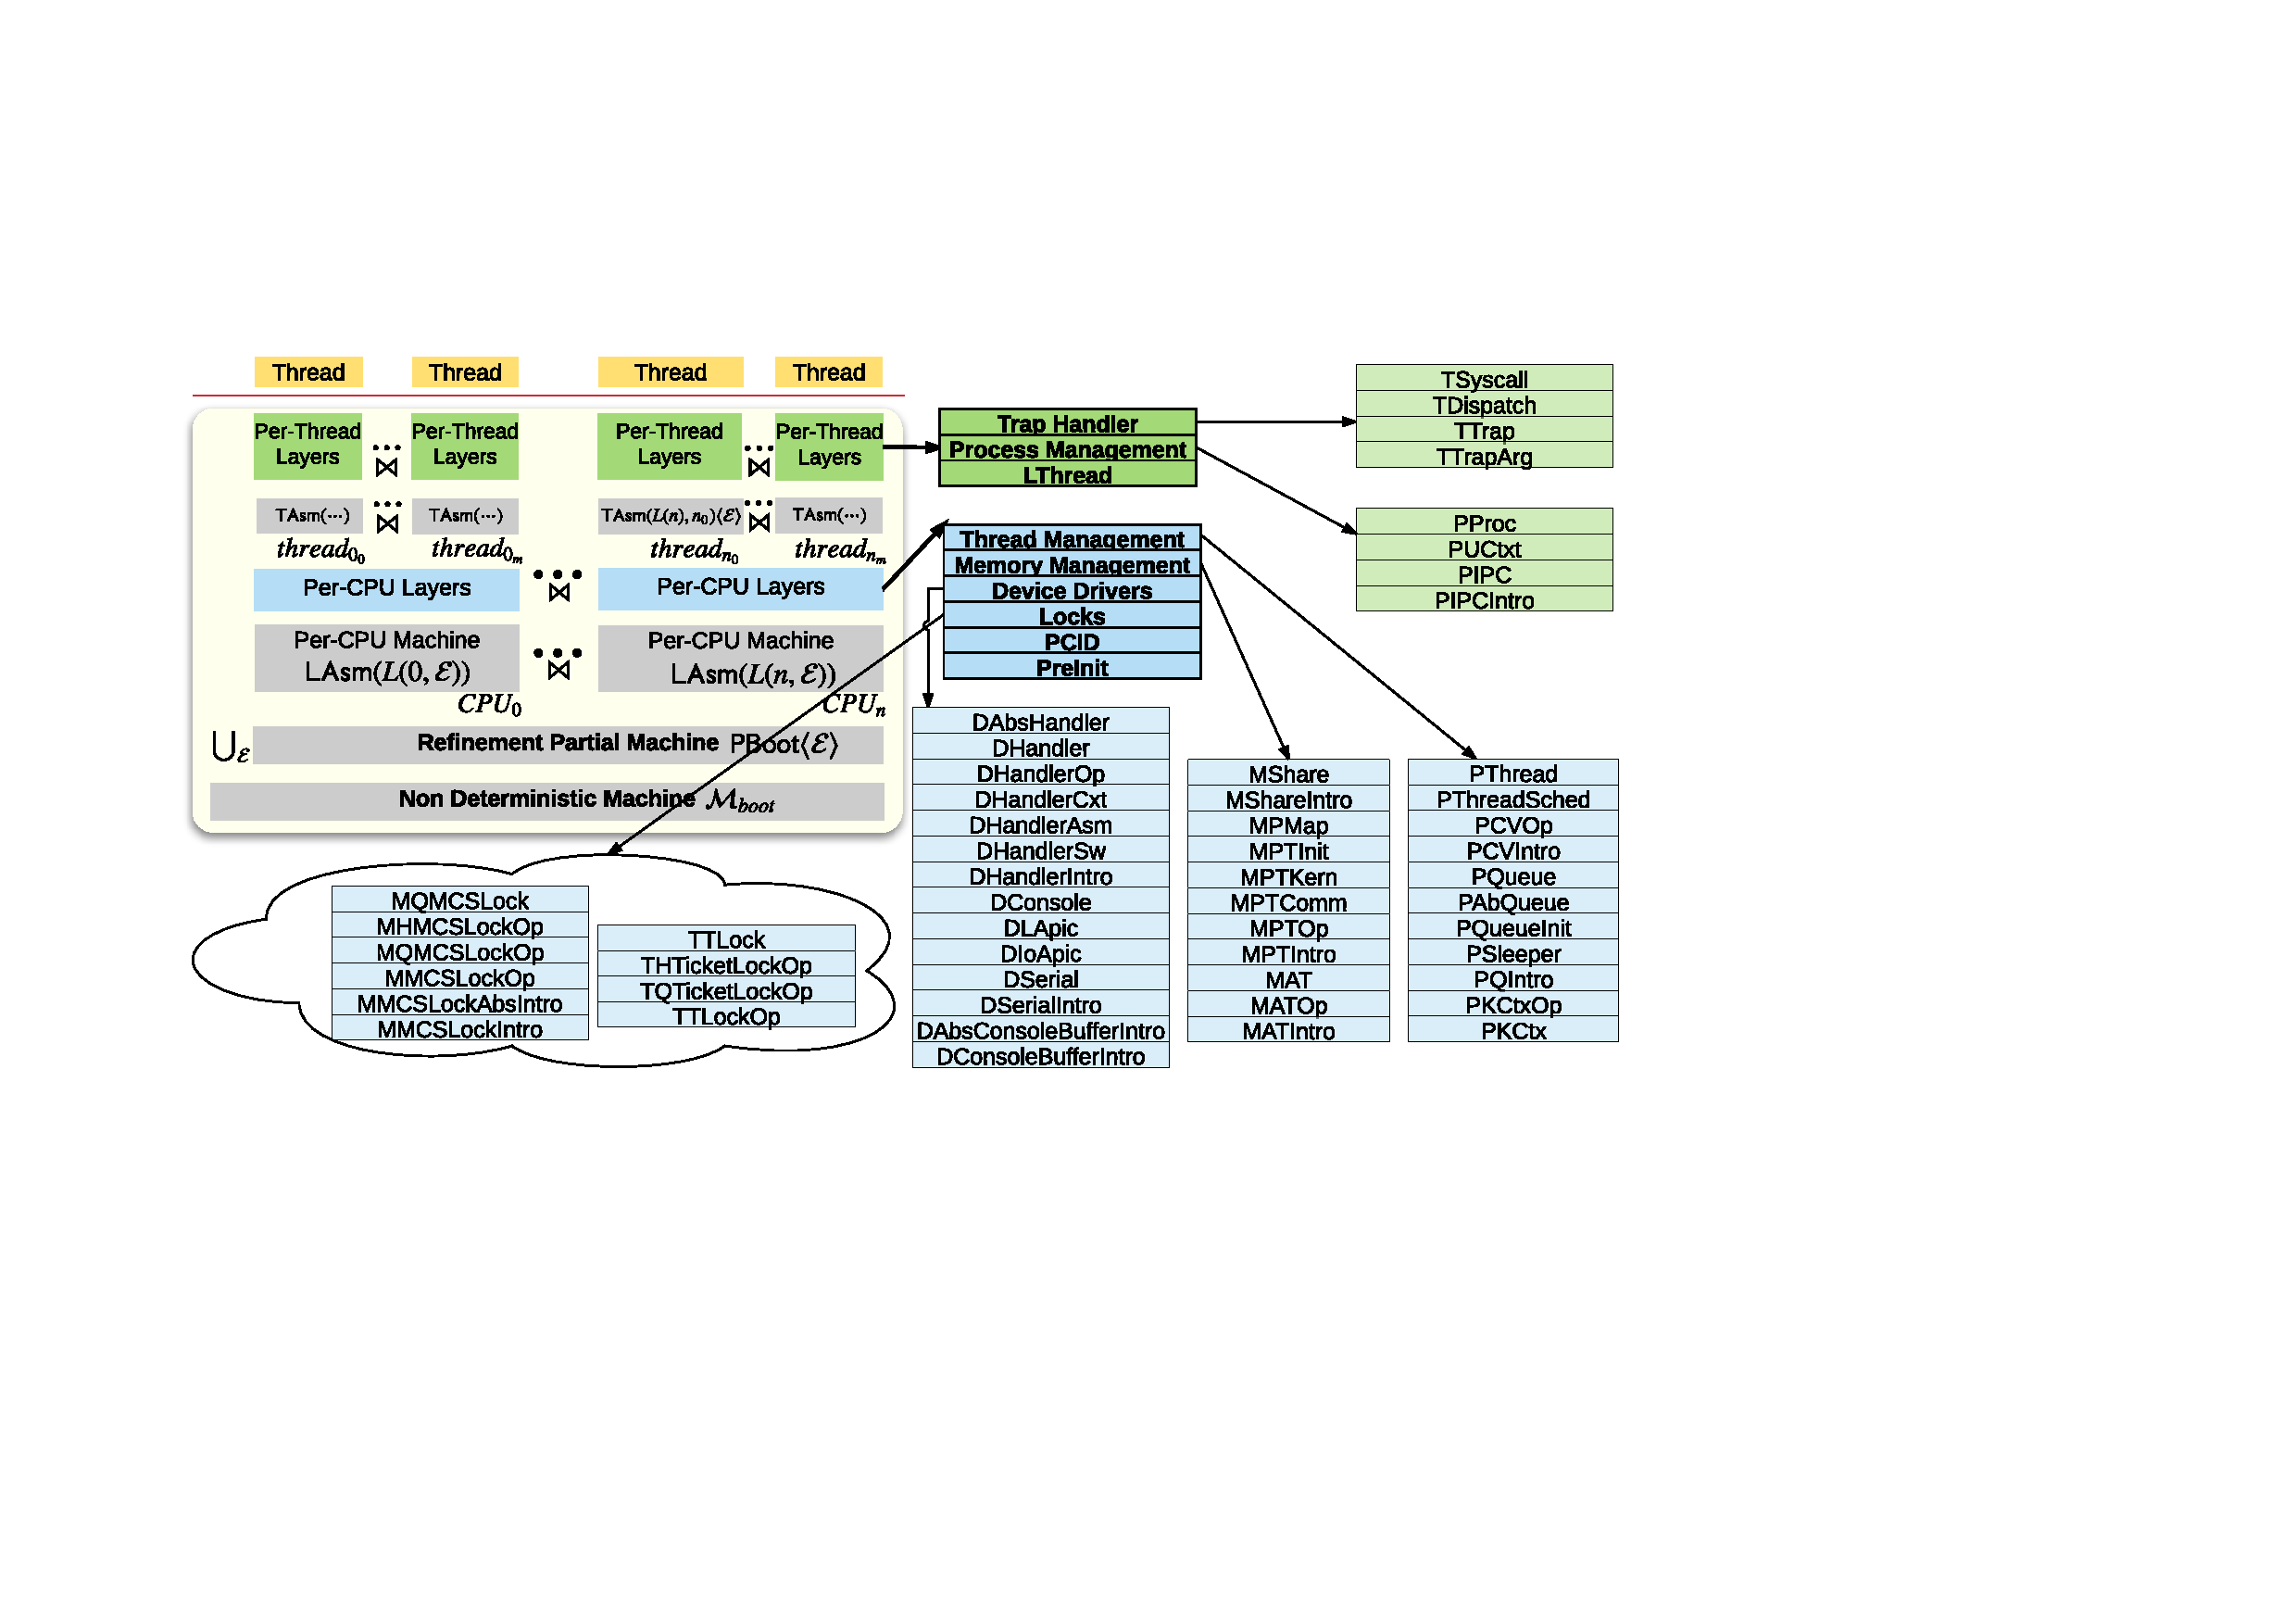
\includegraphics[scale=0.1]{figs/layer_diagram.png}
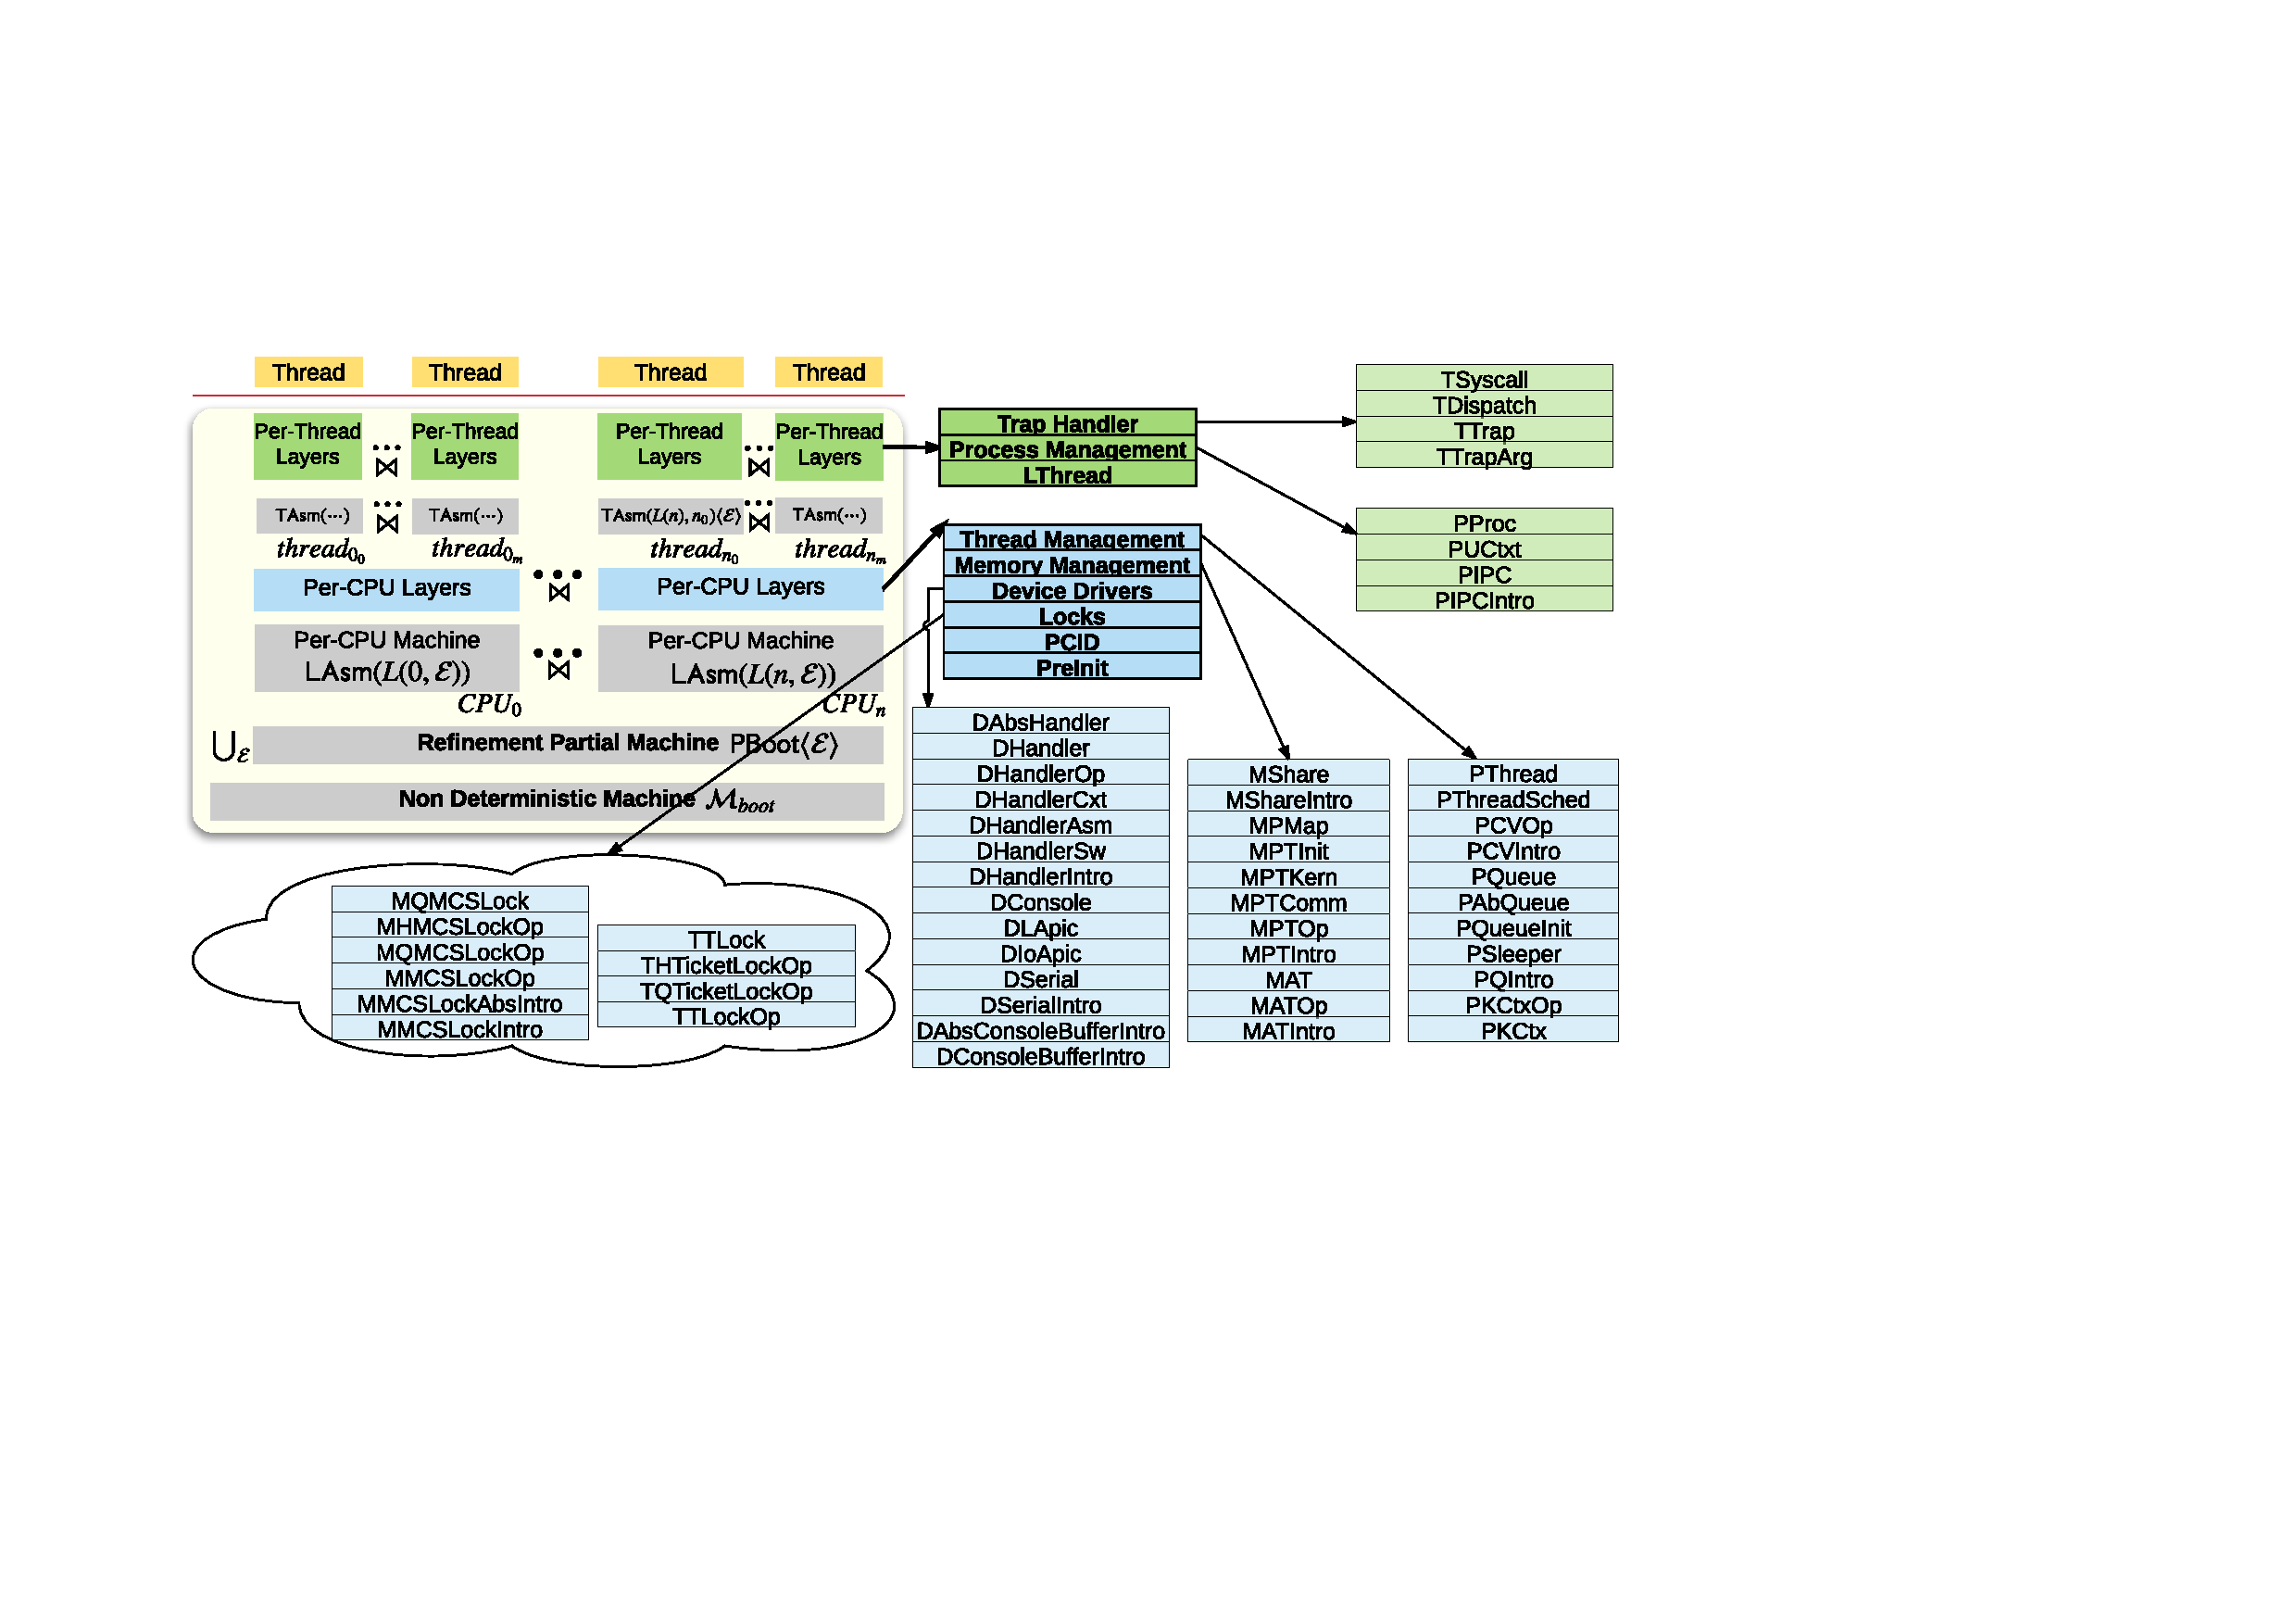
\includegraphics[width=1.0\textwidth]{figs/layer_diagram.pdf}
\vspace{-20pt}
\caption{Layer hierarchy of \cCTOS{} kernel}
\label{fig:layer_diagram}
\vspace{-10pt}
\end{figure*}

We demonstrate our new technology
by extending the \mCTOS{} single-core verified kernel \cite{dscal15} into a
concurrent kernel \cCTOS{} running on multi-core hardware.
In addition to all the concurrent objects described in Sec. \ref{sec:prog},
the kernel also implements an MCS lock \cite{mcs91}, paging-based dynamically
allocated virtual memory,
a synchronous inter-process communication (IPC) protocol implemented using the
queuing lock, and a shared-memory IPC protocol with a shared page.
Using the techniques and strategies presented in the paper, we have
successfully specified and verified the \cCTOS{} kernel in the Coq proof assistant.

Fig.~\ref{fig:layer_diagram} shows the layer hierarchy of  \cCTOS{}.
The gray boxes denote machine models, on top of which the
per-CPU (blue) and per-thread (yellow) layers are built. Orange boxes
are user threads.

The bottom-left portion of the figure illustrates the contextual refinement
among machine models, where we gradually turn the nondeterministic
multicore machine model with arbitrary interleavings
among different processors into a CPU-local machine model that is parameterized
over the behaviors of other processors,
where the switch points only appear at shared operations. This new machine
model allows us to reason about programs running on different processors locally,
and later compose them formally to reason about the whole program.

On top of this abstract machine model, the code of the concurrent kernel is specified and 
verified through 59 abstraction (logical) layers. For each CPU,
we introduce the atomic (ticket and MCS) spinlock objects following
the techniques presented in Sec.~\ref{sec:prog}.
On top of that, the device drivers running inside kernel are verified.
Then there are multiple layers used to introduce memory management units,
the thread context, atomic queue object, and scheduler methods (\cf Sec.~\ref{sec:prog}).
The \texttt{PThread} layer is the topmost layer built for a particular processor.
There, the scheduler primitives like \texttt{yield} and \texttt{sleep}
are specified in a small-step manner, similar to how they are implemented
in C and assembly. Their specifications do not follow the C calling conventions
and thus cannot be called by C code. Above \texttt{PThread}, we then build up the 
per-thread layers that support thread-local reasoning for each CPU.
We first introduce the layer \texttt{PHThread} which defines big-step semantics for
the scheduler primitives that can be invoked from the C level (\cf Sec.~\ref{sec:prog}).
Finally, above the \texttt{PHThread} layer, we verify the
IPC and trap handler modules.

The verified kernel source code (both C and assembly) is extracted using 
Coq's extraction mechanism. The C source code is then compiled by the
extracted verified compiler and merged with the extracted assembly source to
produce the final assembly source code for our verified concurrent kernel. 

\paragraph{Verification Effort and Lessons Learned}
Our team completed verification of the \cCTOS{} kernel in about 2 person years.
The layered approach is key to the scalability and feasibility of such a
large-scale verification effort.
One benefit of our approach is that
concrete and highly optimized (and thus complex) implementations can be abstracted
into much simpler logical specifications that are easier to reason about,
\eg, abstracting a queue implemented as a doubly-linked list into a simple logical list,
abstracting two-level page tables into a logical map from virtual addresses
to physical addresses with permissions, {\it etc}.
Besides this straightforward benefit, the layered approach shines in many other
aspects of complex system verification.

Layering allows us to perform incremental refinement of machine
  models. Real world CPUs are far from ideal for reasoning
purposes, so we abstract the realistic
machine model into a simpler one.
As indicated in Fig.~\ref{fig:layer_diagram}, the per-CPU layers are built on top
of an abstract machine model that supports CPU-local reasoning. Through
multiple contextual refinements, we have proved that the underlying
nondeterministic hardware machine model refines the abstract model. Furthermore, 
because each layer in our framework
is an abstract machine, we can do this not just at
the bottom, but at any point within the verification stack. For example, 
during the \cCTOS{} verification, we first abstract the two-level page table structure
in memory into a logical map from virtual addresses to physical addresses
with permissions. After doing this, we \emph{then} abstract the low level machine 
model that implements page-based virtual memory as described in the hardware 
manual into a simpler model using our abstract logical map.

Layering eases code verification in the concurrent setting.
It allows us to separate code verification from logical reasoning.
Concurrent program verification can be treated as a process of building
verified atomic objects. Each method of an atomic object is implemented using
locks and other atomic objects introduced at lower layers.
When we verify the function body of such a method, we first simply treat it as 
if it were sequential; this results in a non-atomic specification that allows
multiple events to occur. Then, through a separate contextual refinement
that does not involve any code verification, we abstract the environment
context to obtain a new, atomic specification generating only a single event.
In this way, we manage to cleanly separate concurrency reasoning 
(e.g., interleaved executions) from code verification.

\ignore{
{\it Layering facilitates the invariant preservation proof.}
Invariant preservation proofs represent one of the most expensive
components of large-scale verification projects \cite{klein2009sel4}.
They are expensive because they need to be proved not only locally, but
also for the global execution of the whole program. Additionally, many low 
level data manipulation functions temporarily break invariants and reestablish them
later. In our layered approach, every global in-memory data
structure refines one or more isolated abstract logical states in
higher layers. This results in automatic isolation guarantees, despite the
fact that underlying implementations at lower layers still manipulate pointers to
the data structure. Furthermore, each abstraction layer may have a different set
of invariants in our framework, so invariants are introduced incrementally.
For example, consider a queue implemented as a doubly-linked list in
memory. If we directly impose the invariant that the queue is always
well-formed, then we need to prove that no other pointer manipulation in the kernel 
breaks this invariant, while also dealing with the situation where low level 
code temporarily breaks but then reestablishes the invariant. 
Instead, we first abstract
the concrete implementation of the queue into a simple logical list, hiding
concrete pointer manipulation beneath abstract read/write primitives.
Then at higher layers, we gradually introduce and verify the
abstract \texttt{enqueue} and \texttt{dequeue} operations that utilize these
read/write primitives. The well-formedness invariant is only introduced at this 
layer where the \texttt{enqueue} and \texttt{dequeue} operations are atomic and 
all the lower level primitives are already hidden. 
}


\ignore{
\newman{Don't read further. Below are just some random sentences got cut from the OSDI version.}

Furthermore, note that we did not reach the current working solution
in one shot. We first spent about 3 person months developing an
unsuccessful version of the framework for composing multi-threaded
execution on a single CPU.  In that version, thread-local execution
was modeled using a \emph{time stamp} index into a global system
log. We eventually realized that the exact time stamps were too
cumbersome and revealed too much information about the underlying
implementation (\eg, the number of software yields within a function
body), so we spent another month developing a new system that uses
local logs (lists of events) instead.\ignore{ of time stamps, and the
  ability to shuffle and merge the events in the local logs to hide
  unnecessary nondeterminism or implementation details.}  Our initial
multicore machine model also did not work out very well when we
developed the multicore linking framework; we spent 3 person weeks to
improve the initial design through multiple iterations.  The main
challenge was finding the right invariants for the environment
context, such that we could successfully establish starvation-freedom.

\paragraph{Abstraction Layers}
\newman{I am gonna write some summary about the layered approach after I read
the overview section to see how much of the concepts are already covered.}
\begin{itemize}
\item Abstraction of data representation: doubly-linked list --> logical list
\item Stronger invariants
\item Abstraction of primitive specification: hiding log implementation by linking and merging events
\item Refinement of machine models: from a realistic machine model to an ideal machine model that is suitable for our reasoning purpose, e.g., change in machine/memory/interrupt model
\end{itemize}

The verification effort roughly falls into three categories: layer
design with specification and invariants, refinement proofs between
the layers, and verification of C and assembly code with respect to
the specifications. The time needed for each of the categories depends
largely on the layer.  For instance, at the boundary of physical and
virtual memory management (\texttt{MPTIntro}), almost all effort
is in the refinement proof, due to the proof for the refinement between
two completely different memory models. More effort went into the
refinement proof when we introduced the Intel \emph{virtual machine
memory model}, where we proved the refinement between the concrete
four level extended page table structure in memory and the abstract
mapping from the guest addresses to the host addresses.
In contrast, for the layer \texttt{MATOp},
which initializes physical memory allocation,
most of the time was spent on verifying
the non-trivial nested loops present in the C code,
while the refinement proofs were derived automatically. 

The proofs were facilitated by automation tools for C
code, layer design patterns, and tactics libraries developed in
recent years \cite{dscal15}. These tools have greatly
reduced the amount of work needed to verify extensions of the kernel.


Verification not only
should not hinder application of similar performance optimizations,
but instead provide a safety net for more aggressive optimizations, if
it is required for application scenarios of the kernel we have in
mind.
}
    % Case Study: Concurrent CertiKOS (1.5 pages)
\chapter{Limitations and Future Work}
\label{chap-limits}
%\sectskip
%\asectskip

%\zhong{
%Here we address all potential loose-ends.
%\begin{itemize}
%\item any lessons learned?
%\item concurrency and contextual refinement
%\item liveness properties 
%\item compcert memory references vs. capabilities (security properties)
%\item resource usages (stack usages)
%\item interrupts and interrupt handler
%\end{itemize}
%}


\paragraph{Trusted computing base (TCB)}
Currently, there is still some gap between the machine model we rely on and he real x86 hardware.
In the sequential setting,
the bottommost layer of our
verified kernel, {$L_\code{PreInit}$}, does not model
some  hardware features (\eg, TLB) and virtualization
instructions (\eg, \code{vmrun}, \code{vmload}, \code{vmsave}). 
These hardware features can be gradually introduced into our framework in the future. Thanks to the horizontal composition,
these features and newly introduced primitives can be lifted to the related layers with minimal changes to the rest.

In the concurrent settting,
our assembly machine $\mach{x86mc}$ assumes strong sequential consistency for all
atomic instructions. Nevertheless, our proof remains valid for the x86
TSO model. All our concurrent layers guarantee that non-atomic memory
accesses are properly synchronized.  The TSO order guarantees that all
atomic synchronization operations are properly ordered (and there is
no need to insert any explicit fences).  \citet{vontessin13} shows how
to turn proofs over sequential-consistent machines into those over
the TSO machines.

Outside our verified kernels
(\cCTOS{} consists of about 6000 lines of C and assembly), there
are 300 lines of C and 170 lines of x86 assembly code that are not
verified yet: the ELF loader used by user
process creation
and the preinit procedure, which initializes the drivers, \eg,
disk, console, {\etc}
Although these primitives touches lots of low-level details,
they can be decomposed into multiple phases and verified by building 
a stack of layers below $L_\code{PreInit}$.
The verification of these modules 
is left for future work. 

\ignore{Device drivers are not verified
because our current machine semantics lacks device models for
expressing the corresponding semantics.}

Finally, the CompCert assembler for converting assembly into machine
code is also not verified. We also assume the correctness of the Coq
proof checker and its code extraction mechanism.

%The following is no longer accurate: now these switches are fully
%verified.
%% \item some assembly code generated for the switches between ring0
%% and ring3, and between the host and the guest. Our machine
%% semantics % ($\LSem{L}$) models these switches as pseudo
%% primitives. They can be verified if we model more detailed hardware
%% behaviors and instructions in our machine model.
%% C functions, such as memcpy, are not supported by the current 
%% CompCert memory model and thus can not be verified in $\ClightX{L}$.
%% On the other hand, they can be implemented in assembly and verified 
%% at the assembly level, which we leave for future work.
% Do we really have any code in the kernel (I mean, apart from the
% bootloader and preinit) having the following features?
%% \item Some C features are not supported by the current CompCert, e.g.
%% functions with varying number of arguments, and the GCC-style inline
%% assembly. They could be verified in assembly, which we leave for future work.

\paragraph{Expressivity of context code} 
Our assembly machine only covers a small part of the full x86
instruction set and hardware features, so our contextual correctness results only apply to
programs in this subset. Additional instructions 
can be easily added if they have simple or no interaction with our
kernel.  \citet[Section 6]{costanzo16} shows how the fidelity of the
CompCert-style x86 machine model would impact the formal correctness
or security claims, and how such gap can be closed.


\ignore{
\paragraph{Concurrency}
Our current certified kernels assume a runtime environment consisting
of a single processor, but extending it to support multicore
concurrency is already under way. Our choice of using contextual refinement 
to connect layers is motivated partly by its
deep connection with the work on concurrent
objects~\cite{herlihy90,herlihy08book}.

In \CTOS, all primitives introduced at each abstraction layer are
assigned ``atomic'' specifications. Such ``atomicity'' is easy to
establish in the sequential setting when interrupts are turned off.
In the concurrent setting (and even with preemption and all the
interleavings), we would still want the underlying kernel
implementation module to behave like its sequential counterpart 
in all contexts. This is the essence of {\em linearizability}~\cite{herlihy90}.

Recent work on concurrency verification~\cite{liang13,filipovic10} has
shown that contextual refinement is precisely equivalent to
linearizability. In fact, by
varying the observable context and the assumption about the scheduler,
Liang~{\em{}et al}~\cite{liang13} have shown that termination-sensitive
contextual refinement (which we use in \CTOS) is precisely equivalent
to linearizability plus a specific liveness property (i.e., 
wait-freedom, lock-freedom, obstruction-freedom, starvation-freedom
or deadlock-freedom).

These results suggest that by using contextual
refinement, \CTOS\ can isolate and encapsulate fine-grained concurrent
interleavings inside the implementation of each kernel object within a
single layer. Non-blocking fine-grained concurrent data structures can have
very sophisticated local invariants, but they are not exported to
other parts of the kernel. This makes the \CTOS\ architecture much
more appealing and extensible.}

\paragraph{Preemptive interrupt} Like most existing verified kernel efforts,
we do not allow preemptive interrupts inside the kernel. The
challenges in handling preemption are similar to those
for concurrency. 
We plan to model different devices
as virtual CPUs
and utilize the hardware scheduler
to capture the
preemptive interrupts between devices and the kernel.

\paragraph{Storage system}
All our kernels currently lack a certified storage system.
%and a certified network stack.
%The Linux community~\cite{lkmap} sorted these
%into different stacks of abstraction layers (based on their underlying
%hardware devices).\vilhelm{it's not clear to me what point this sentence makes.}
We plan to incorporate recent advances in building
certified file systems~\cite{fscq15,cogent16} into \mCTOS{} and \cCTOS\ in the near future.

\paragraph{Linking across layers before compiling}
In our current framework, all the modules are compiled
 within their own layer interfaces and linked together at the assembly level. Thus, we cannot inline functions across layers and ``getter-setter"
 layers introduce performance overhead.
 
Actually, our layer
calculus does provide ways to first link code at the C level across
layers before compiling. Let $L_3$ be an overlay, $L_1$ be an
underlay, and $L_2$ be an intermediate layer interface. Let us assume that we
split each layer interface $L_i$ into two layer interfaces $L_i^C \oplus
L_i^{\mathrm{Asm}}$ and that we proved $L_{i}^{\mathit{lang}} \vdash_{R_i}
M_i^{\mathit{lang}}: L_{i+1}^{\mathit{lang}}$ for each $i \in \{1,2
\}$ and $\mathit{lang} \in \{ C, \mathrm{Asm} \}$.

Then, on each side, we can do vertical composition and obtain
$L_1^{\mathit{lang}} \vdash_{R_2 \circ R_1} M_1^{\mathit{lang}} \oplus
M_2^{\mathit{lang}} : L_3$. We can then follow the process described
in Section~\ref{sec:linking} with $H = L_3$, $L = L_1$ and
$M^{\mathit{lang}} = M_1^{\mathit{lang}} \oplus M_2^{\mathit{lang}}$, so that we obtain:
\[
L_1 \vdash_{R_2 \circ R_1} \mathrm{CompCertX}(M_1^C \oplus M_2^C) \oplus M_1^{\mathrm{Asm}} \oplus M_2^{\mathrm{Asm}}: L_3
\]
This shows that compiling before linking is possible as soon as
ClightX supports vertical composition with refinement. 
Recall that the soundness proof for the vertical composition rule in Section~\ref{sec:seq:sound}
requires the monotonicity of $\oplus$ and the language semantics $\llbracket - \rrbracket$.
For ClightX,
the
corresponding Coq proof for monotonicity is underway. 
Once it is proved, because CompCertX already
supports function inlining (within a single module) just like CompCert
does, if an intermediate layer interface defining ``getter-setters'' is to be
implemented through simple functions performing only a single memory
access, then compilation before linking will allow suppressing the
function call overhead for these simple functions. 
As they are linked
within a single module before compilation, so that memory accesses
will be inlined in the overlay implementation.



% This part is mostly covered in Section 5 now, we shouldn't need it anymore
\begin{comment}
\paragraph{Security and information flow}
We also plan to utilize the extensible, layered framework of
\CTOS{} to guarantee that information flow or security properties are never
broken by a valid layer implementation. For example, consider proving
a variant of the end-to-end confidentiality property known in the
literature as \emph{noninterference}. Informally, the property says
that the observable behavior of a program is independent of the
initial values of some particular high-security data (i.e., there is
no flow of information from the high-security data to the observable
events produced by the program). We define the specification of a
program as the (partial) mapping from initial state to final state,
and call a specification ``noninterfering'' if it satisfies the
property just described. Our goal is then to prove that, at any layer
$L_i$, if all the primitives implemented in layer $L_{i-1}$ have
noninterfering specifications, then a program written in layer
$L_i$ using those primitives will also be noninterfering. We
have found that such a goal is achievable via instrumentation of the
CompCert-style memory model with security labels, and
intelligently placed label checks within the operational
semantics. Note that these security labels are abstract state---they
do not actually exist in the concrete machine, and thus they do not
add any execution overhead.

We also intend to leverage our \CTOS\ architecture to generalize the
integrity and noninterference properties of seL4~\cite{murray13,sewell11}
beyond the purely access-control-based policy that parameterizes the 
properties. Rather than explicitly storing pieces of an access control 
policy in capabilities and passing them between kernel objects, we wish 
to reason about label-based policies via a purely static instrumented 
machine. Another way to view this goal is with respect to the HiStar 
operating system~\cite{zeldovich06}. In HiStar, all kernel objects have
an attached security label. Label checks are performed during kernel 
execution to prevent undesirable information flows, though no formal 
guarantees regarding information flow are stated or proved. Our goal 
can be viewed, then, as taking HiStar's security labels, migrating them 
from the actual machine into the realm of static verification, and 
proving extensible, end-to-end information-flow guarantees. Through this 
process, we also anticipate that security policies (given through 
specifications) will become clearer and more declarative.
\end{comment}

\ignore{
\paragraph{Evaluation and limitations} 
The planning and development of \mCTOSbase{} took 9.5 person months plus
2 person months on linking and code extraction.
With the infrastructure in place, \mCTOShyper{} only took 1.5 person months
to finish, and \mCTOSringz{} and \mCTOSembed{} take half a person month each.
The kernels are written, layer by layer, in LAsm and ClightX abstract syntaxes
along with driver functions specifying how to compose (link) them.
All of those are in Coq for the proofs to refer to.
We utilize Coq's code extraction to get an OCaml program which contains
CompCertX, the abstract syntax trees of the kernels, and the driver functions,
which invoke CompCertX on pieces of ClightX code and
generate the full assembly file.
The output of the OCaml program is then fed to an assembler to produce
the kernel executable.

With the device drivers (running as user processes) and a cooperative 
scheduler, most of the benchmarks in
lmbench\footnote{\url{http://lmbench.sourceforge.net/}}
are under 2x slowdown running in \mCTOShyper{},
well within expected overhead.
Ring 0 processes, not used in the above experiment, can 
easily lower the number
as we measured one to two orders of magnitude reduction in the number of cycles
needed to serve system calls and context switches.

Because the proof was originally developed directly in terms of
abstract machines and program transformations,
the current code base does not yet reflect the calculus presented in
Sec. \ref{sec:layer} in its entirety.
%The most significant discrepency is that the simulation relations blueprints
%used by our legacy code do not actually compose.%
%\footnote{
%  This is not a fundamental limitation of our approach,
%  but merely a technical difficulty due to the way
%  the compiler's memory injections are integrated to
%  the definition of these relations
%  in our pre-existing code base.
%  % XXX: Please refer to the technical report for more 
%  % complete explanation.
%}
% Expand in technical report:
%  The simulation relations need to factor in the peculiar form of the
%  compiler's correctness theorem
%  (XXX: refer somehow to Sec. \ref{sec:comp.tex}),
%  and consequently are parametrized over Compcert memory injections.
%  In order to define the composition $(R_1 \circ R_2)(j)$ from
%  $R_1(j_1)$ and $R_2(j_2)$,
%  we would need to find a way to split $j$ into $j_1$ and $j_2$
%  XXX: explain more
Notably,
vertical composition is done at the level of
the whole-machine contextual refinements
obtained by applying the soundness theorem
to each individual abstraction layer.
%[XXX: Talk about simulation paths, refactoring to address this issue?]

Outside our verified kernels
(\mCTOShyper{} consists of about 3000 lines of C and assembly), there
are 300 lines of C and 170 lines of x86 assembly code that are not
verified yet: the preinit procedure, the ELF loader used by user
process creation, and functions such as \textsf{memcpy} which currently
cannot be verified because of a limitation arising from the CompCert
memory model. Device drivers are not verified because LAsm
lacks device models for expressing the correctness
statement.  Finally, the CompCert assembler for converting LAsm into
machine code remains unverified. 
%We also assume the correctness of the
%Coq proof checker and its code extraction mechanism.

LAsm does not cover the full x86 instruction sets and many other
hardware features.  This means that our correctness results only apply
to programs in this subset. However, additional instructions and
features can be easily added if they have simple or no interaction
with our kernel.}



\section{Implementation and Deployment}
\label{sec:eval:impl}
%\section{Implementation}
%\label{sec:imp}

\paragraph{Coq implementation}

After we finished the verification of different OS kernels presented
here, we have employed an exhaustive clean-up process to improve our
layered specification and verification framework.  Our initial Coq
implementation required verifying the contextual version of the
{\em implements} relation at each layer.  While such layer refinement
proofs followed some fixed patterns, the proof process heavily relied
on copying and pasting the existing templates and filling in the
missing proof holes.  The copy and paste approach also brought some
code and proof duplication.  In the new implementation, we instead
verify the per-primitive {\em implements} relation and then rely on the
soundness theorem of the layer calculus to turn this relation into the
contextual version. The contextual correctness property is derived
from the monotonicity of the client context in the carrier language.

We have also implemented more automation tactic libraries to further
ease the task of the verification. We are able to automate the majority of
tasks in the code verification and refinement proofs by extensively
applying these tactics. For the code verification, these tactics are
used for automatic definition unfolding, rewriting of terms, proving
that primitive calls never fault, verification condition generation,
and other first-order theorem proving to discharge the verification
conditions.  For the refinement relation, we developed a decision
procedure that automatically applies the layer calculus rules to split
the layer refinement into per-function forward simulations.  As for
the per-function forward simulation, getter-setter functions and
pass-through primitives are proved completely by tactic automations.
In the future, we are also interested in implementing horizontal
composition with framing to substitute the pass-through primitives.
We also built some extra libraries to prove x86 addressing modes and
the specification properties required by the layer calculus and
CompCertX.  Furthermore, we have extended the arithmetic
tactic \texttt{omega} with integer division and modulus.  Coq's
Ltac language is untyped, thus fixing a formal layer calculus helped a
lot in stabilizing these tactic libraries.

In our first approach, we tried to bundle the abstract data together
with the invariants on them using dependent types. This made the
automation of proofs more difficult as every time a new instance is
constructed, the framework requires us to explicitly construct a proof
that the new data satisfies the invariants. In our new approach, we
handle the invariants separately, and thus the invariants no longer
appear in the semantics of the primitives nor in the verification of
the programs. Then, we prove the layer interface invariant
preservation once and for all by showing that the initial abstract
data satisfies the invariants and all the semantics of the primitives
preserve the invariants. This proof makes sure that the layer
interface invariants are preserved during any execution, for all
programs (including the context) running on top of the layer
interface.


\paragraph{Proof effort}
With the help of the layer calculus and automation libraries
introduced in the new implementation, we successfully reduced the work
of adding one new layer from 4,000 lines of Coq code to 500 lines on
average.  The rough compilation time for a layer was reduced from a
few minutes to less than a minute.

The verification effort roughly falls into three categories: layer
design with specification and invariants, refinement proofs between
the layers, and verification of C and assembly code with respect to
the specifications. The time needed for each of the categories depends
largely on the layer.  For instance, at the boundary of physical and
virtual memory management ({$L_\code{MPTIntro}$}), almost all effort
is in the refinement proof, due to the proof for the refinement between
two completely different memory models. More effort went into the
refinement proof when we introduced the Intel \emph{virtual machine
memory model}, where we proved the refinement between the concrete
four level extended page table structure in memory and the abstract
mapping from the guest addresses to the host addresses.
In contrast, for the layer {\code{MATOp}},
which initializes physical memory allocation,
most of the time was spent on verifying
the non-trivial nested loops present in the C code,
while the refinement proofs were derived automatically. 

The proofs were facilitated by automation tools for C
code, layer design patterns, and tactics libraries developed in
recent years \cite{dscal15}. These tools have greatly
reduced the amount of work needed to verify extensions of the kernel.
\ignore{
\jeremie{I do not understand what the following sentence mean
(developing the module vs. ``plugging'' it),
I'm also not sure how it fits with the previous one,
I suggest we just drop it (or move it to Sec.5) and end the paragraph here.}
For example, developing the Intel virtualization module as a certified
kernel plug-in cost over 2 pm. However, plugging this module into
\mCTOSbase{} was done within a person week. \ignore{It took another 2 pm to
link all the proofs together and extract a runnable \mCTOShyper{}
assembly code using the Coq's extraction mechanism.} Modifying and
removing the existing modules does not take much effort either, as
demonstrated by the realization of \mCTOSringz{} and \mCTOSembed{},
which cost 0.5 pm each.
}



\paragraph*{Deployment}
An extended version of \mCTOShyper{} was deployed in context of a large
DARPA-funded research project. It runs on a military land vehicle
using the same hardware configuration we used in the experiments. On
top of the extended version run 6 Ubuntu Linux systems as guests. Each virtual
machine runs several RADL (The Robot Architecture Definition Language)
nodes that have fixed hardware capabilities such as access to GPS,
radar, \etc\\

\ignore{
This section describes our Coq implementation and provides some
actual evaluation of our various efforts. The main point of this
section to show that everything we have talked about so far are
actually real.

List of potential topics/discussions.
\begin{itemize}
\item Challenges met in the Coq implementation.
\item Particular interesting issues or challenges we met during the proof.
\item Any interesting topics we want to talk about in the proof.
\item How the new language constructs eased the task of verification/automation.
\item How we handle invariants. And how separating the invariants from the data helped the automation.
\item Bugs found?
\item Any implementation specific topics?
\item We we designed the layers.
\item Kernel specific challenges and/or interesting topics.
\item Modularity and scalability of our layered approach. How easy it was to extend the kernel with various new constructs?
\item Decide what to submit and acknowledge the work in progress and possible improvements.
\item \emph{anybody want to add more potential items here?}
\end{itemize}
}

\ignore{
\paragraph{Limitations and perspective}
We also try to enumerate all the important limitations of our current
effort. We want to address all possible questions typical readers of
our paper might have and explain why these issues can and will be
addressed in the future. 
}


\ignore{
\begin{figure}\small
\begin{center}
\begin{tabular}{|c|c|}
%\hline
%\multicolumn{2}{|l|}{Development of ClightX and CompCertX} & 10 pm \\
\hline
Physical memory module (3 layers) &  2 pm \\
\hline
Virtual memory module (7 layers) & 2.5 pm \\
\hline
Thread management (10 layers) & 3.5 pm \\
\hline
Process management (4 layers) & 1 pm \\
\hline
Trap handler module (3 layers) & 0.5 pm \\
\hline
\hline
Virtualization (9 layers) for \mCTOShyper{} & 1.5 pm \\
\hline
Changes for \mCTOSringz{}  & 0.5 pm \\
\hline
Changes for \mCTOSembed{}  & 0.5 pm\\
\hline
Linking and code extraction & 2 pm \\
\hline
\end{tabular}
\end{center}
\caption{Effort on verification}
\label{fig:effort}
\end{figure}
}

\ignore{
As shown in Fig.~\ref{fig:effort}, we completed the entire
verification effort of \mCTOS{} in less than 12 person months (pm).  At the
beginning, it took more than 2pm to design and verify the three layers
of physical memory management.  After the proof libraries (e.g. VCGen,
layer design pattern, tactics libraries \textit{etc}.) have been
developed, the average time of designing and verifying one layer was
dramatically reduced. On the verification side, one line of C code can
be proved within 30 lines of Coq code, while one line of assembly
requires only 20 lines of proof.
}



\chapter{Evaluation and Lessons Learned}
\label{chap-eval}
To evaluate
our CertiKOS framework
and a series of verified kernels,
we have analyzed the performance  the  \cCTOS{} concurrent kernel
with a thorough experimental benchmark evaluation.
Furthermore, an extended version of \cCTOS{}
was deployed in a practical system that is used in the context of a
large DARPA-funded research project. 
Section~\ref{sec:eval:perform} shows our experiments with benchmarks, which
confirm the observations made during deployment: the performance
overhead of \cCTOS{} is moderate. 
In Section~\ref{sec:eval:impl},
we presents the implementation and deployment of
our verified kernels.
All in all, we are convinced that it is
practical to use our verification framework to produce competitive
real-world kernels with acceptable effort.


\section{Performance Evaluation} 
\label{sec:eval:perform}
Although the performance is not the main
emphasis of this thesis, we have run a number of micro and macro
benchmarks to measure the speedup and overhead of {\cCTOS} and to
compare {\cCTOS} to existing systems such as KVM and seL4. All
experiments have been performed on an Intel Core i7-2600S (2.8GHz,
4~cores) with 8~MB L3 cache, 16~GB memory, and a 120~GB
Intel 520 SSD. Since the power control code has not been verified, we
disabled the turbo boost and power management features of the hardware
during experiments.


\paragraph{Concurrency overhead} The run-time overhead introduced by concurrency
in {\cCTOS} mainly comes from \emph{the latency of spinlocks} and
\emph{the contention of the shared data}.

The {\cCTOS} kernel provides two kinds of spinlocks: ticket lock and
MCS lock. They have the same interface and thus are
interchangeable. In order to measure their performance, we put an
empty critical section (payload) under the protection of a single
lock. The latency is measured by taking a sample of 10,000 consecutive
lock acquires and releases (transactions) on each round.

\begin{figure}\centering
	\hspace{-.2cm}
	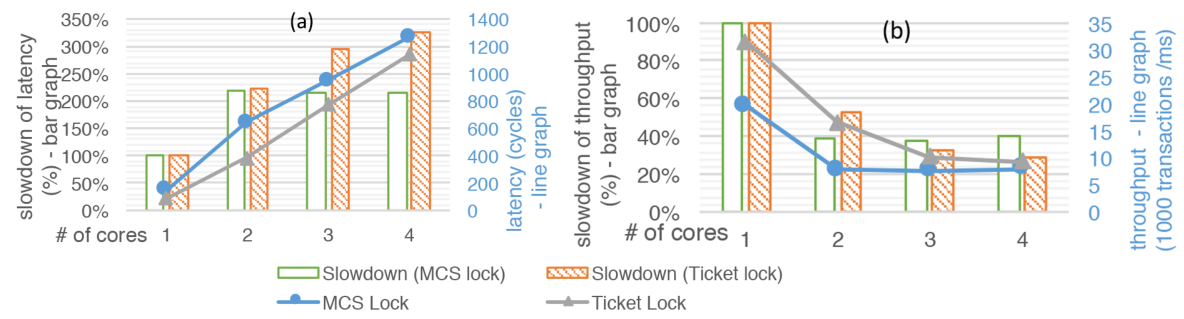
\includegraphics[width=10cm]{figs/locks.pdf}
	\hspace{-.2cm}
	\caption{The comparison between actual efficiency of ticket lock and MCS lock implementations in \cCTOS{}.}
	\label{fig:locks}
\vspace*{-10pt}        
\end{figure}

Figure~\ref{fig:locks} shows the results of our latency
measurement. In the single core case, ticket locks impose 34 cycles of
overhead, while MCS locks impose 74 cycles (line chart).
%%%%%%%%%%%%%%%%%%%%
\ignore{\hao{These numbers are larger
than normal spinning locks implementation. It is caused by the overhead of
additional primitive calls when we split the lock operation into multiple
layers.} \newman{Let's leave the numbers and comments for this for now.
Let's see if Hao can get the new performance data out before we submit
the report tonight. If not, we will revert the numbers back to the
old ones and add appropriate comments.}}
%%%%%%%%%%%%%%%%%%%%
As the number of cores grows, the latency increases rapidly. However,
note that all transactions are protected by the same lock. Thus, it is
expected that the slowdown should be proportional to the number of
cores. In order to show the actual efficiency of the lock
implementations, we normalize the latency against the baseline (single
core) multiplied by the number of cores ($\frac{n*t_1}{t_n}$). As can
be seen from the bar chart, efficiency remains about the same for MCS
lock, but decreases for ticket lock.

Now that we have compared MCS lock with ticket lock, we present the
remaining evaluations in this section using only the ticket lock
implementation of \cCTOS{}.

To reduce contention, all shared objects in {\cCTOS} are carefully
designed and pre-allocated with a fine-grained lock.
\ignore{
For example,
the {\cCTOS} process scheduler on each CPU does not need to access any
shared data if no relevant process is sleeping.
}
We design a benchmark
with server/client pairs to evaluate the speedup of the system as more
cores are introduced.  
We run a pair of server/client processes on each
core, and we measure the total throughput (i.e., the number of
transactions that servers make in each millisecond) across all
available cores.
%%%%%%%%%%%%%%%%
%In this benchmark, we run three pairs of server/client processes
%on all available cores, and we measure the total
%throughput (i.e., the number of transactions that servers make in each
%millisecond) across all the cores.
%%%%%%%%%%%%%%%%
A server's transaction consists of first performing an IPC receive
from a channel $i$, then executing a payload (certain number of
`\texttt{nop}' instructions), and finally sending a message to channel
$i + 1$. Correspondingly, a client executes a constant payload of 500
cycles, sends an IPC message to channel $i$, and then receives its
server's message through channel $i + 1$.  When the client has to wait
for a reply from the server, the control is switched to a special
system process which then immediately yields back to the server
process.

\begin{figure}\centering
	\hspace{-.2cm}
	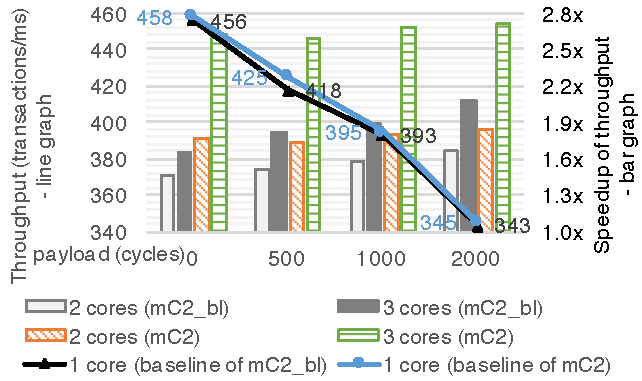
\includegraphics[width=10cm]{figs/speedup_big_lock2.pdf}
	\hspace{-.2cm}
	\caption{Speedup of throughput of \cCTOS{} vs. {\cCTOS-bl} in a client/server benchmark under various server payloads (0-2,000).}
	\label{fig:speedup_big_lock}
\end{figure}

Figure~\ref{fig:speedup_big_lock} shows this server/client benchmark,
comparing {\cCTOS} against a big-kernel-lock version of {\cCTOS}
({\cCTOS-bl}). We insert a pair of lock acquire and release at the
top-most layer by hand, and replace all fine-grained locks with an
empty function. This does not introduce bias because the speedup is
normalized against its own baseline (single core throughput) for each
kernel version separately. From the figure, we can see that the
speedup rate for big-kernel-lock is about 1.45x $\sim$ 1.66x with 2
cores and 1.64x $\sim$ 2.07x with 3 cores. On the other hand, the
fine-grained locks of {\cCTOS} yield better speedup as the number of
cores increases (roughly 1.77x $\sim$ 1.84x and 2.62x $\sim$ 2.71x
with 2 and 3 cores, respectively). Note that the server/client pairs
are distributed into different CPUs, and there is no cross core
communication; therefore, one might expect perfect scaling as the
number of cores increases.  However, we do not quite achieve perfect
scaling because each core must execute some system processes which run
at constant rates and consume some CPU resources, and we did not align
our kernel data structures against cache-line size.

\ignore{
\begin{figure}\centering
	\hspace{-.2cm}
	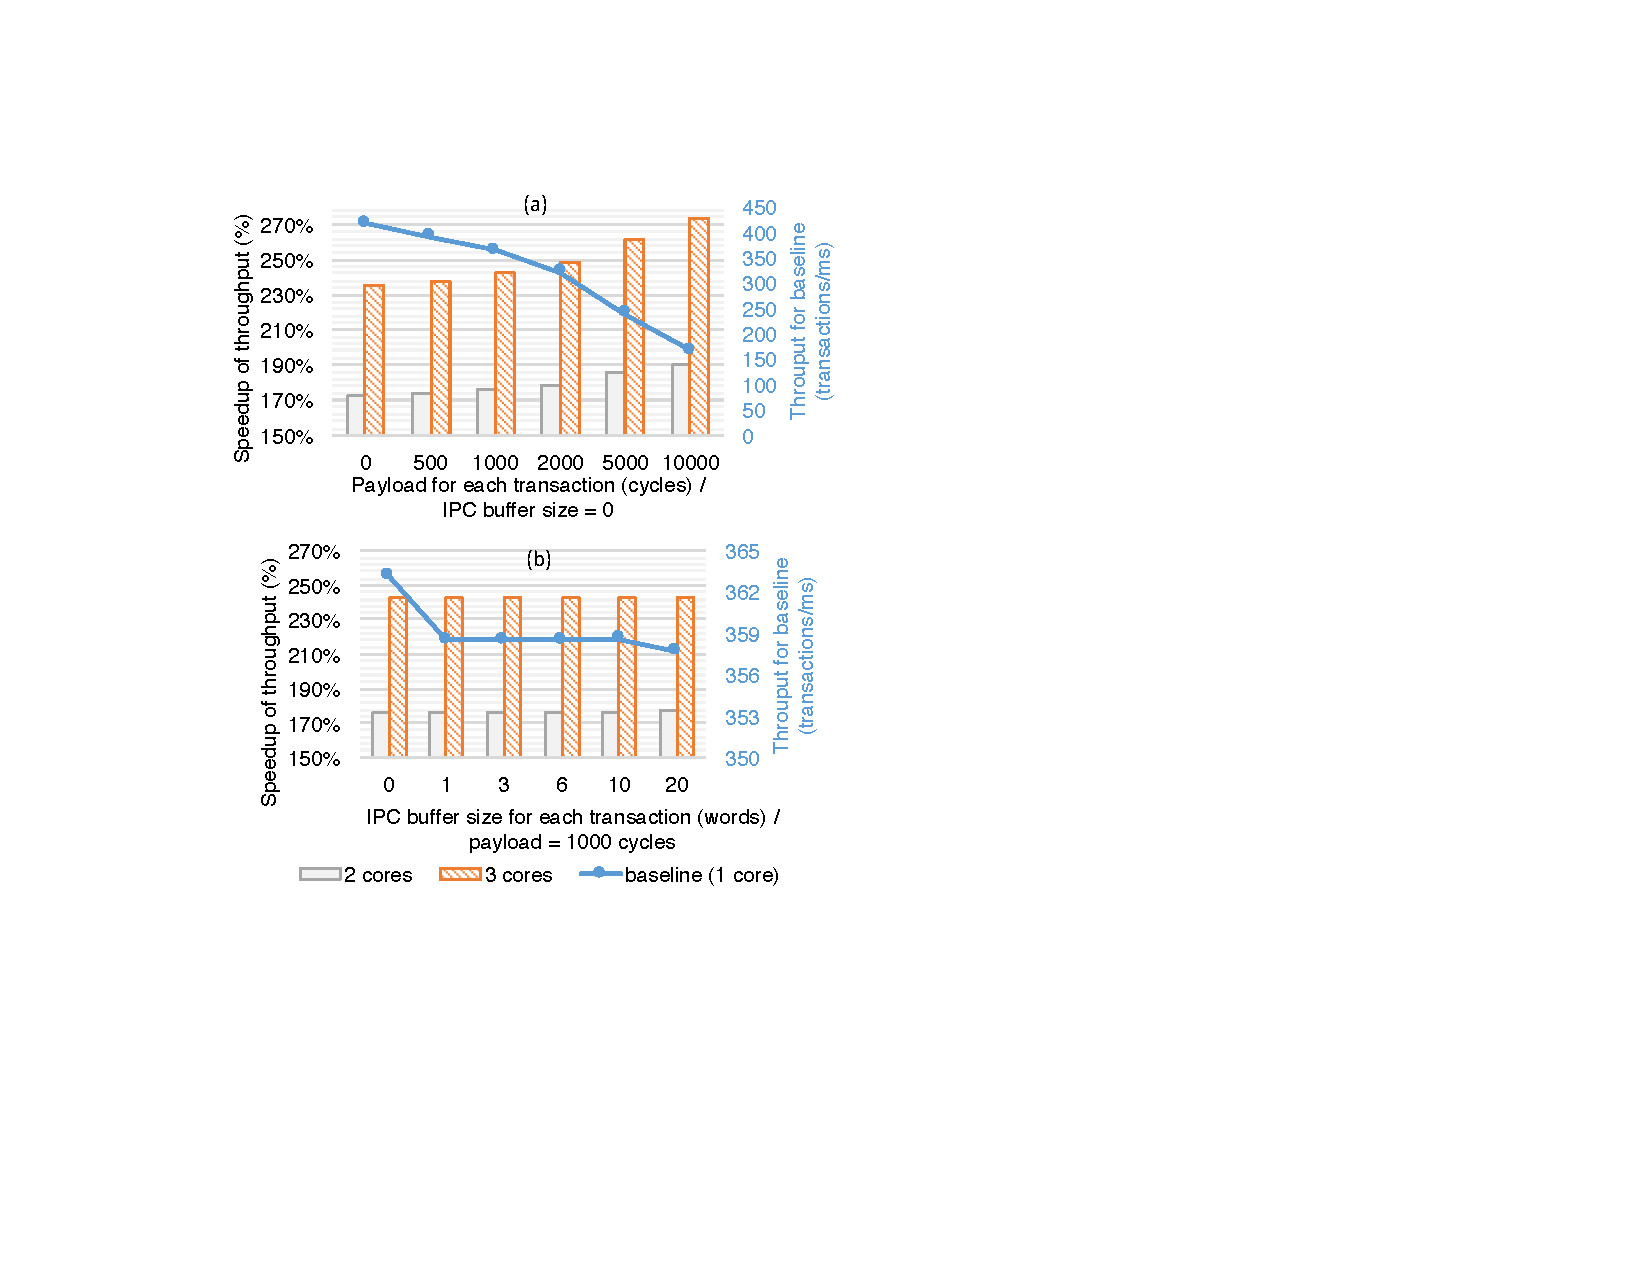
\includegraphics[width=6cm]{figs/speedup_pb.pdf}
	\hspace{-.2cm}
	\caption{Speedup of the throughput of \cCTOS{} in 2 and 3 cores against various server payloads (0 - 10,000) and IPC message sizes (0 - 20).}
	\label{fig:speedup_pb}
\end{figure}

Figure~\ref{fig:speedup_pb} shows the speedup of {\cCTOS} against various
server payloads and IPC message sizes. Figure~\ref{fig:speedup_pb} (a) shows that
the throughput decreases along with the increase of the server
workload (from I/O intensive task with payload being 0 to computation intensive task with
payload being 10,000) in the line chart. However, the speedup (bar chart) is increasing,
ranging from 1.7x to 1.9x for 2 cores, and 2.3x to 2.7x for 3 cores. The reason
is that the execution of the payload does not require the access to any shared
data, thus the contention becomes less intense. In
Figure~\ref{fig:speedup_pb} (b), the throughput decreases slightly when the
IPC message size increases, but the speedup is not affected.
}


\paragraph{IPC Performance} We measure the latency of IPC send/recv in {\cCTOS}
against various message sizes, and compare the result with seL4's IPC
implementation.

A comparison of the performance of seL4 and \cCTOS{} is not
straightforward since the verified \cCTOS{} kernel runs on a multicore
x86 platform, while the verified seL4 kernel runs on ARMv6 and ARMv7
hardware and only supports single-core. Thus, we use an unverified,
single-core version of seL4 for comparison. Moreover, the synchronized
IPC API in seL4 (\texttt{Call/ReplyWait}) has a different semantics
from \cCTOS{}'s send/recv: it uses a round-trip message passing
protocol (with a one-off reply channel created on the fly) while
trapping into the kernel twice, and it does not use any standard sleep
or wakeup procedures. To have a meaningful comparison with respect
to the efficiency of implementing system calls, we compare
$(send + recv) \times 2$
of \cCTOS{} with
${(Call + ReplyWait) + Null \times 2}$ of seL4,
where $Null$ is the latency of a null system call in seL4.

We measure seL4's performance using seL4's IPC benchmark
sel4bench-manifest~\cite{sel4bench} with processes in different
address spaces and with identical scheduler priorities, both in
\emph{slowpath} and \emph{fastpath} configurations. We consulted the
seL4 team~\cite{heiser16} and used 158 cycles as the cost of each null
system call ($Null$) in seL4. To measure \cCTOS{}'s performance, we
simply replace seL4's \emph{Call} and \emph{ReplyWait} system calls
with {\cCTOS}'s synchronous \emph{send} and \emph{receive} calls. We
found that, when the buffer size is zero, \cCTOS{} takes about 3800
cycles to perform a round trip IPC, while seL4's fastpath IPC takes
roughly 1200 cycles, and seL4's slowpath IPC takes 1800 cycles. When
the message size is larger than 2 words, the fastpath IPC of seL4
falls back to the slowpath; in the 10-words IPC case, \cCTOS{}'s round
trip IPC takes 3820 cycles, while seL4 takes 1830 cycles.
%%%%%%%%
\ignore{Considering \cCTOS{} requires two more system calls than
  seL4,\cCTOS{}'s IPC is slightly slower than seL4's.}
%%%%%%%%
Note that seL4 follows the microkernel design philosophy, and thus its
IPC performance is critical. IPC implementations in seL4 are highly
optimized and heavily tailored to specific hardware platforms.
%%%%%%%%
\ignore{The IPC performance of \cCTOS{} is still practical. Verification not
	only should not hinder application of similar performance optimizations, but
	instead provide a safety net for more aggressive optimizations, if it is
	required for application scenarios of the kernel we have in mind.}

\ignore{
	On {\cCTOS}, the performance of inter-core IPC is worse than that of
	intra-core IPC.  The reason is that, after the receiver thread is
	woken up, it is first pushed onto the \emph{pending queue} of the
	corresponding CPU, which gets pushed back to the scheduler's ready
	queue at the subsequent scheduling point. Furthermore, as shown in the
	figure, the performance of the send call is not affected by the buffer
	size. That is because the send system call simply saves the virtual
	address and size of the user buffer into the channel.  The actual
	copying of data is all done by the receive call.  Before copying the
	data, the receive call needs to switch the page map to an identity
	map, copy the data, and switch the page map back before it goes back
	to user. Note that switching page map causes TLB flushes, which
	imposes extra performance overhead to the receive call in addition to
	the overhead of copying the data.

\begin{figure}\centering
	\hspace{-.2cm}
	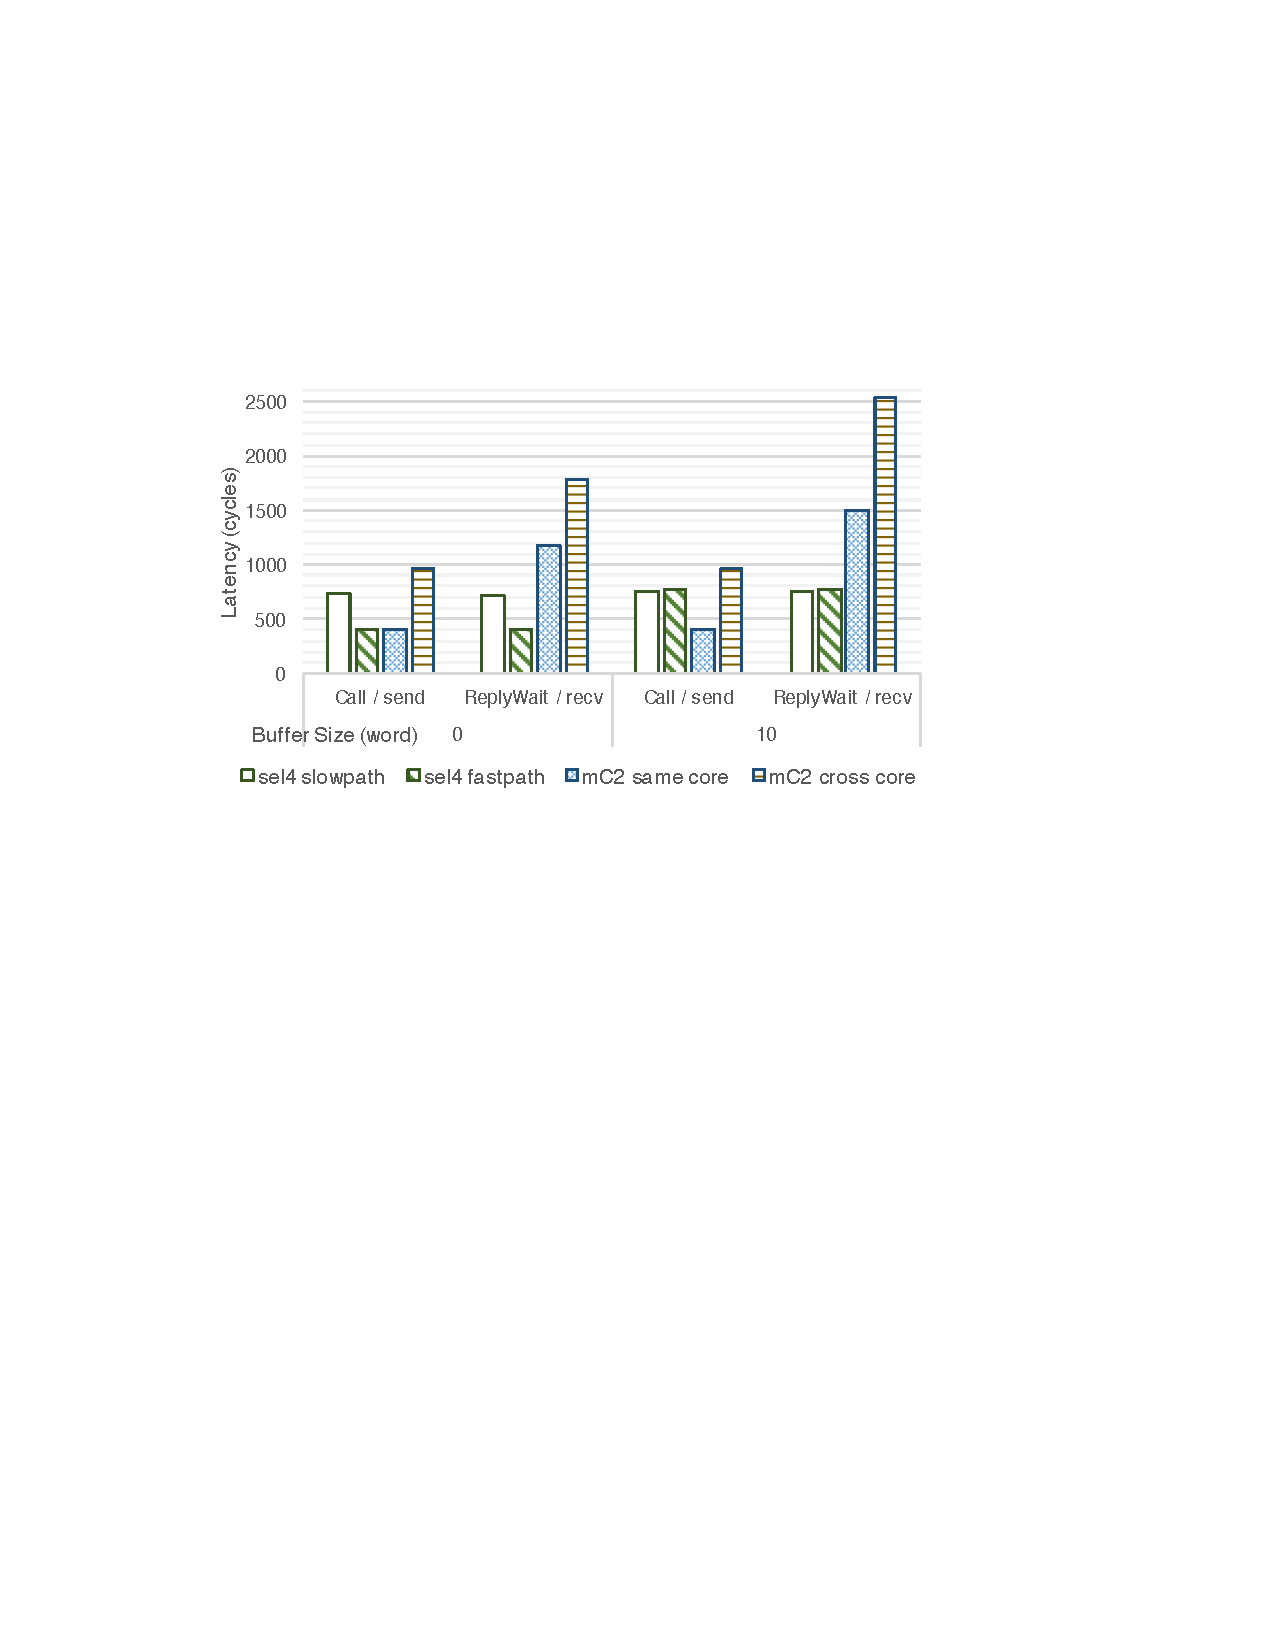
\includegraphics[width=8cm]{figs/ipc.pdf}
	\hspace{-.2cm}
	\caption{IPC performance between \cCTOS{} and  seL4 x86.}
	\label{fig:eval_ipc}
\end{figure}

}


\paragraph{Hypervisor Performance} 
\begin{figure}\centering
		\hspace{-.2cm}
		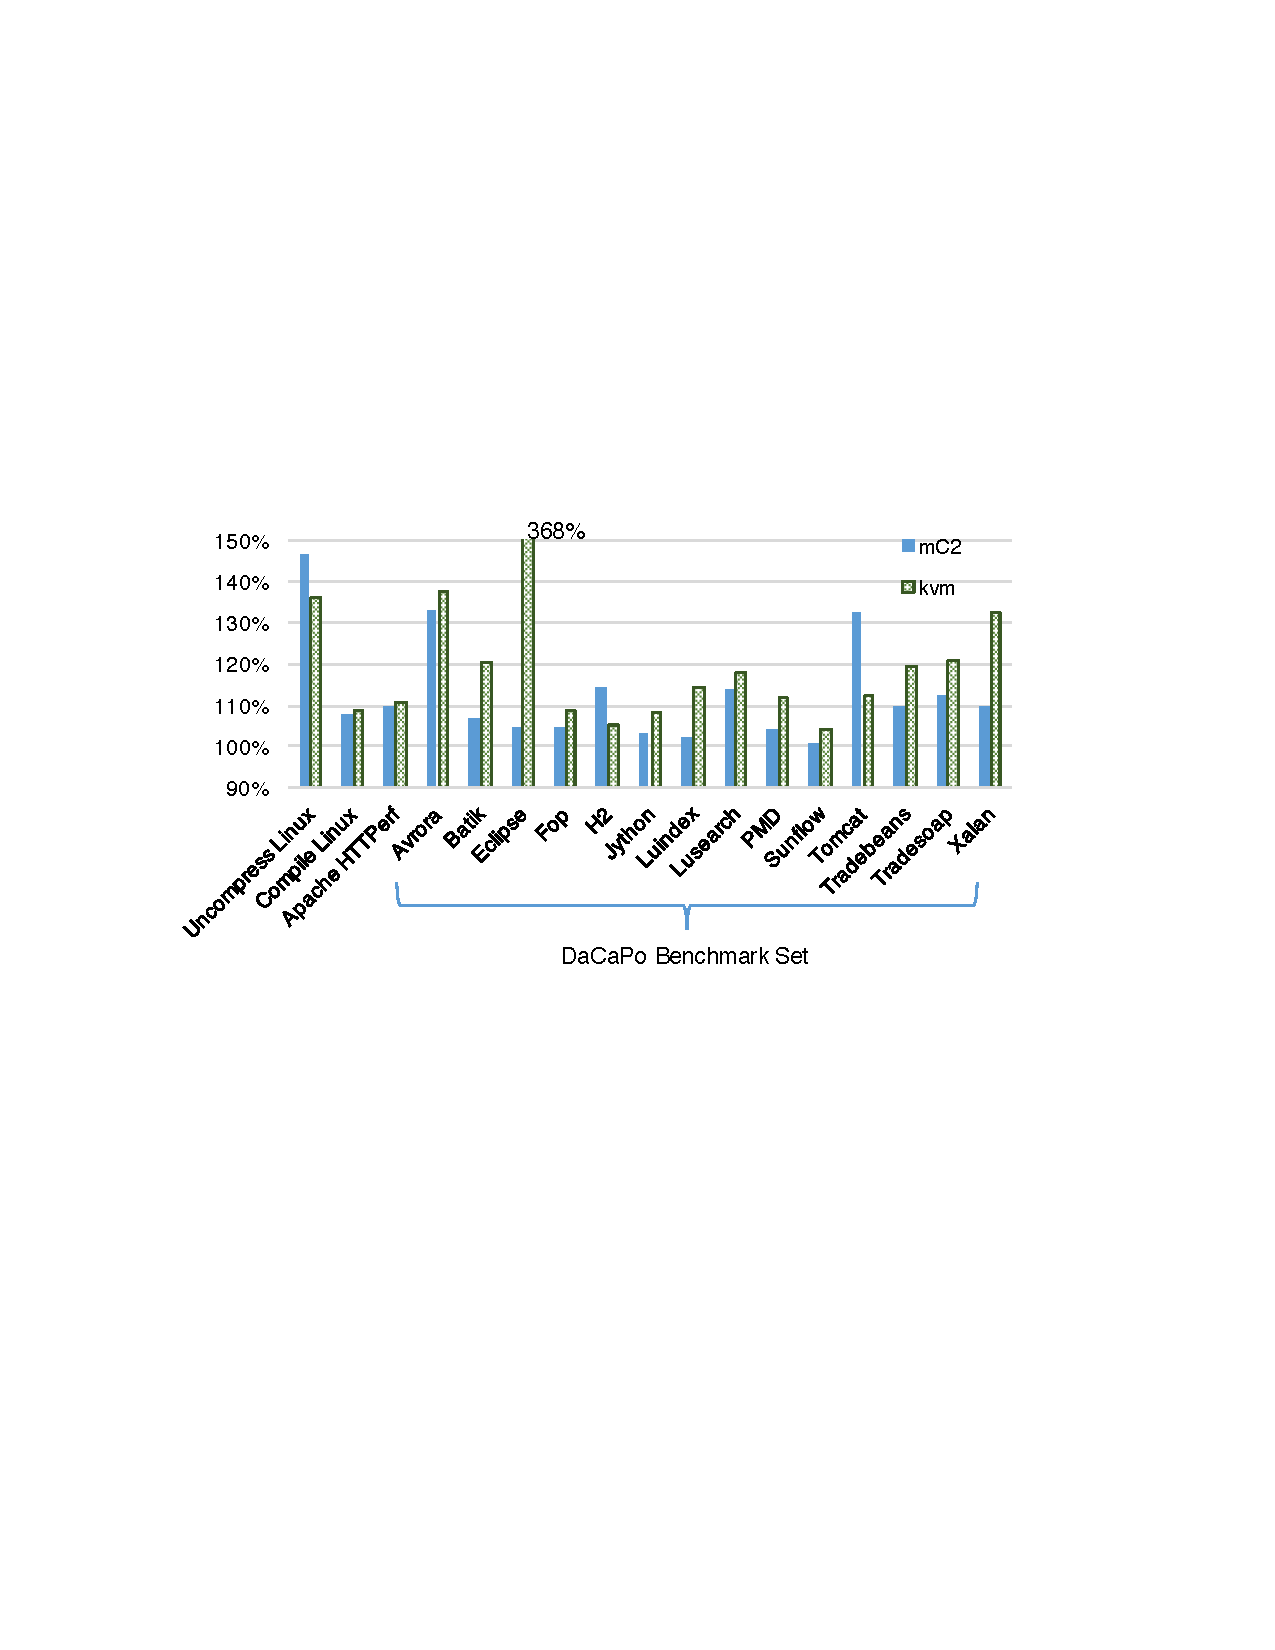
\includegraphics[width=13cm]{figs/hyp_macro.pdf}
		\hspace{-.2cm}
		\caption{Normalized performance for
                         macro benchmarks running over Linux on KVM
                         vs. Linux on \cCTOS; the baseline is
                         Linux on bare metal;
                         a smaller ratio is better.}
		\label{fig:eval_macro}
\end{figure}

To evaluate \cCTOS{} as a hypervisor, we measured the performance of some macro
benchmarks on Ubuntu 12.04.2 LTS running as a guest.  We ran the benchmarks on
Linux as guest in both KVM and \cCTOS{}, as well as on the bare metal. The guest
Ubuntu is installed on an internal SSD drive. KVM and \cCTOS{} are installed
on a USB stick. We use the standard 4KB pages in every setting~--- huge pages are not used.


 \ignore{Although there is an unverified branch of seL4 that supports
   VT-x, the verified version does not have virtualization support and
   cannot boot Linux. As a result, we do not compare hypervisor
   performance but instead focus on a comparison of the IPC
   performance of {\cCTOS} and an \emph{unverified} x86 version of
   seL4.}

Figure~\ref{fig:eval_macro} contains a compilation of standard macro
benchmarks: unpacking of the Linux 4.0-rc4 kernel, compilation of the
Linux 4.0-rc4 kernel, Apache HTTPerf~\cite{mosberger1998} (running on
loopback), and DaCaPo Benchmark 9.12~\cite{dacapo2006}.
%%%%%%%%%
\ignore{
To begin with a sanity check, McVoy's LMbench (version 3-alpha1) is used to
measure the micro-level metrics of operating system and hardware, which includes
the bandwidths and latency of several file system, local communication systems,
virtual memory, context switch and, basic arithmetic operations. The results
show that 34 out of 60 benchmarks of \cCTOS{} are very close to the bare
metal (within the range of 5\%), and the others are listed in the Table \hao{we need a talbe?}. These
results shows that there is no significant overhead of \cCTOS{}.
	}
%%%%%%%%%
% In Figure~\ref{fig:eval_macro}, w
%%%%%%%%%
We normalize the running times of the benchmarks using the bare metal
performance as a baseline (100\%). The overhead of \cCTOS{} is
moderate and comparable to KVM. In some cases, \cCTOS{} performs
better than KVM; we suspect this is because KVM has a Linux host and
thus has a larger cache footprint.  For benchmarks with a large number
of file operations, such as Uncompress Linux source and Tomcat,
\cCTOS{} performs worse. This is because \cCTOS{} expose the raw disk
interface to the guest via VirtIO~\cite{russell08} (instead of doing
the pass-through), and its disk driver does not provide good buffering
support.








\section{Implementation and Deployment}
\label{sec:eval:impl}
%\section{Implementation}
%\label{sec:imp}

\paragraph{Coq implementation}

After we finished the verification of different OS kernels presented
here, we have employed an exhaustive clean-up process to improve our
layered specification and verification framework.  Our initial Coq
implementation required verifying the contextual version of the
{\em implements} relation at each layer.  While such layer refinement
proofs followed some fixed patterns, the proof process heavily relied
on copying and pasting the existing templates and filling in the
missing proof holes.  The copy and paste approach also brought some
code and proof duplication.  In the new implementation, we instead
verify the per-primitive {\em implements} relation and then rely on the
soundness theorem of the layer calculus to turn this relation into the
contextual version. The contextual correctness property is derived
from the monotonicity of the client context in the carrier language.

We have also implemented more automation tactic libraries to further
ease the task of the verification. We are able to automate the majority of
tasks in the code verification and refinement proofs by extensively
applying these tactics. For the code verification, these tactics are
used for automatic definition unfolding, rewriting of terms, proving
that primitive calls never fault, verification condition generation,
and other first-order theorem proving to discharge the verification
conditions.  For the refinement relation, we developed a decision
procedure that automatically applies the layer calculus rules to split
the layer refinement into per-function forward simulations.  As for
the per-function forward simulation, getter-setter functions and
pass-through primitives are proved completely by tactic automations.
In the future, we are also interested in implementing horizontal
composition with framing to substitute the pass-through primitives.
We also built some extra libraries to prove x86 addressing modes and
the specification properties required by the layer calculus and
CompCertX.  Furthermore, we have extended the arithmetic
tactic \texttt{omega} with integer division and modulus.  Coq's
Ltac language is untyped, thus fixing a formal layer calculus helped a
lot in stabilizing these tactic libraries.

In our first approach, we tried to bundle the abstract data together
with the invariants on them using dependent types. This made the
automation of proofs more difficult as every time a new instance is
constructed, the framework requires us to explicitly construct a proof
that the new data satisfies the invariants. In our new approach, we
handle the invariants separately, and thus the invariants no longer
appear in the semantics of the primitives nor in the verification of
the programs. Then, we prove the layer interface invariant
preservation once and for all by showing that the initial abstract
data satisfies the invariants and all the semantics of the primitives
preserve the invariants. This proof makes sure that the layer
interface invariants are preserved during any execution, for all
programs (including the context) running on top of the layer
interface.


\paragraph{Proof effort}
With the help of the layer calculus and automation libraries
introduced in the new implementation, we successfully reduced the work
of adding one new layer from 4,000 lines of Coq code to 500 lines on
average.  The rough compilation time for a layer was reduced from a
few minutes to less than a minute.

The verification effort roughly falls into three categories: layer
design with specification and invariants, refinement proofs between
the layers, and verification of C and assembly code with respect to
the specifications. The time needed for each of the categories depends
largely on the layer.  For instance, at the boundary of physical and
virtual memory management ({$L_\code{MPTIntro}$}), almost all effort
is in the refinement proof, due to the proof for the refinement between
two completely different memory models. More effort went into the
refinement proof when we introduced the Intel \emph{virtual machine
memory model}, where we proved the refinement between the concrete
four level extended page table structure in memory and the abstract
mapping from the guest addresses to the host addresses.
In contrast, for the layer {\code{MATOp}},
which initializes physical memory allocation,
most of the time was spent on verifying
the non-trivial nested loops present in the C code,
while the refinement proofs were derived automatically. 

The proofs were facilitated by automation tools for C
code, layer design patterns, and tactics libraries developed in
recent years \cite{dscal15}. These tools have greatly
reduced the amount of work needed to verify extensions of the kernel.
\ignore{
\jeremie{I do not understand what the following sentence mean
(developing the module vs. ``plugging'' it),
I'm also not sure how it fits with the previous one,
I suggest we just drop it (or move it to Sec.5) and end the paragraph here.}
For example, developing the Intel virtualization module as a certified
kernel plug-in cost over 2 pm. However, plugging this module into
\mCTOSbase{} was done within a person week. \ignore{It took another 2 pm to
link all the proofs together and extract a runnable \mCTOShyper{}
assembly code using the Coq's extraction mechanism.} Modifying and
removing the existing modules does not take much effort either, as
demonstrated by the realization of \mCTOSringz{} and \mCTOSembed{},
which cost 0.5 pm each.
}



\paragraph*{Deployment}
An extended version of \mCTOShyper{} was deployed in context of a large
DARPA-funded research project. It runs on a military land vehicle
using the same hardware configuration we used in the experiments. On
top of the extended version run 6 Ubuntu Linux systems as guests. Each virtual
machine runs several RADL (The Robot Architecture Definition Language)
nodes that have fixed hardware capabilities such as access to GPS,
radar, \etc\\

\ignore{
This section describes our Coq implementation and provides some
actual evaluation of our various efforts. The main point of this
section to show that everything we have talked about so far are
actually real.

List of potential topics/discussions.
\begin{itemize}
\item Challenges met in the Coq implementation.
\item Particular interesting issues or challenges we met during the proof.
\item Any interesting topics we want to talk about in the proof.
\item How the new language constructs eased the task of verification/automation.
\item How we handle invariants. And how separating the invariants from the data helped the automation.
\item Bugs found?
\item Any implementation specific topics?
\item We we designed the layers.
\item Kernel specific challenges and/or interesting topics.
\item Modularity and scalability of our layered approach. How easy it was to extend the kernel with various new constructs?
\item Decide what to submit and acknowledge the work in progress and possible improvements.
\item \emph{anybody want to add more potential items here?}
\end{itemize}
}

\ignore{
\paragraph{Limitations and perspective}
We also try to enumerate all the important limitations of our current
effort. We want to address all possible questions typical readers of
our paper might have and explain why these issues can and will be
addressed in the future. 
}


\ignore{
\begin{figure}\small
\begin{center}
\begin{tabular}{|c|c|}
%\hline
%\multicolumn{2}{|l|}{Development of ClightX and CompCertX} & 10 pm \\
\hline
Physical memory module (3 layers) &  2 pm \\
\hline
Virtual memory module (7 layers) & 2.5 pm \\
\hline
Thread management (10 layers) & 3.5 pm \\
\hline
Process management (4 layers) & 1 pm \\
\hline
Trap handler module (3 layers) & 0.5 pm \\
\hline
\hline
Virtualization (9 layers) for \mCTOShyper{} & 1.5 pm \\
\hline
Changes for \mCTOSringz{}  & 0.5 pm \\
\hline
Changes for \mCTOSembed{}  & 0.5 pm\\
\hline
Linking and code extraction & 2 pm \\
\hline
\end{tabular}
\end{center}
\caption{Effort on verification}
\label{fig:effort}
\end{figure}
}

\ignore{
As shown in Fig.~\ref{fig:effort}, we completed the entire
verification effort of \mCTOS{} in less than 12 person months (pm).  At the
beginning, it took more than 2pm to design and verify the three layers
of physical memory management.  After the proof libraries (e.g. VCGen,
layer design pattern, tactics libraries \textit{etc}.) have been
developed, the average time of designing and verifying one layer was
dramatically reduced. On the verification side, one line of C code can
be proved within 30 lines of Coq code, while one line of assembly
requires only 20 lines of proof.
}



\paragraph{Execution Model and Completeness}
The majority of the {\cCTOS} and \cCTOS{} kernels are implemented and verified 
at the C level and then compiled by a modified version of the CompCert verified
compiler~\cite{dscal15}.  The entire kernel (both C and assembly)
source code, together with the source code for the verified compiler,
are extracted into an OCaml program through Coq's extraction
mechanism. When this OCaml program is executed, the extracted C source code 
is compiled into assembly; the resulting assembly code is then merged 
with the existing assembly kernel source code to produce a single piece 
of assembly code corresponding to our verified kernel.  Thus, our deliverable 
consists of a piece of assembly code for the entire verified kernel, a 
high-level deep specification of various kernel behaviors, and a 
machine-checkable proof object stating that the assembly code running on 
the actual hardware satisfies the high-level specification.

The verified assembly code is then linked with the rest of the kernel code
(the bootloader and remaining unverified drivers) to produce the
actual binary image of the OS. The resulting kernels are practical.

\begin{figure}[t]
\lstinputlisting [language = C, multicols=2] {source_code/fifoq3.c}
\caption{Pseudocode of the remove method for FIFOBBQ}
\label{fig:exp:fifo}
\end{figure}

\paragraph{Bugs found}
Formal verification is a great way to
locate hard-to-find concurrency-related bugs.
For example,  implementing starvation-free condition variables
is not trivial and even the popular, most up-to-date OS
textbook~\cite[Figure~5.14]{ospp11} has gotten it
wrong~\cite{anderson16}.

A \emph{condition variable} (CV) is a synchronization object that
enables a thread to wait for a change to be made to a
shared state (protected by a lock).  Standard Mesa-style
CVs~\cite{lampson80} do not guarantee starvation-freedom: a thread
waiting on a CV may not be signaled within a bounded number of
execution steps. 
Initially, we implemented a version of CV
using condition queues as shown by \citet[Figure~5.14]{ospp11}. However, during the verification,
we have found a bug in the FIFOBBQ implementation shown in that
textbook: in some cases, their system can get stuck by allowing all
the signaling and waiting threads to be asleep simultaneously, or the
system can arrive at a dead end where the threads on the remove queue
(rmvQ) can no longer be woken up.  We fixed this issue by postponing
the removal of the CV of a waiting thread from the queue, until the
waiting thread finishes its work (\cf Figure~\ref{fig:exp:fifo}); the
remover is now responsible for removing itself from the rmvQ (line~24)
and waking up the next element in the rmvQ (line~27). Here, \code{peekQ}
reads the head item of a queue; and \code{my\_cv} returns the CV
assigned to the current running thread. 

Other than the FIFOBBQ bug,
we have also found a subtle bug in  
our initial ticket-lock implementation:   
the spinning loop body (line 10 in Figure~\ref{fig:exp:ticket_lock})
was implemented as
``\lstinline$while($$\intp$\lstinline$L[i].now<t){}$". 
This still passed all our tests, but  
during the verification,
we found that it did not satisfy the atomic specification
since the ticket field might overflow. For example, 
if \lstinline$L[i].ticket$ is $(2^{32}-1)$, \code{acq\_lock} will
cause an overflow (line 9 in  Figure~\ref{fig:exp:ticket_lock}) and
the returned ticket
\lstinline$t$ equals $0$. In this case, 
\lstinline$L[i].now$ is not less than \lstinline$t$ 
and \code{acq\_lock} returns immediately, which violates 
the order implied by the ticket. We fixed this bug by 
changing the loop body to 
``\lstinline$while($$\intp$\lstinline$L[i].now!=t){}$";
we completed the proof by showing that the maximum 
number of concurrent threads is far below $2^{32}$.





\ignore{it
runs on stock x86 hardware and can successfully boot a guest version
of Linux.}

\ignore{\section{Proof effort}
We take the mCertiKOS kernel presented by Gu {\it et al}
\cite{dscal15}, and extend the kernel with various features such as
dynamic memory management, container support for controlling resource
consumption, Intel hardware virtualization support, shared memory IPC,
single-copy synchronous IPC, ticket and MCS lock implementation, new
schedulers, condition variables, FIFO blocking bounded queues, {\it
  etc}. Note that all of these new features are implemented in the
context of a concurrent machine, whereas the mCertiKOS presented by Gu
{\it et al} \cite{dscal15} only runs on a single-core machine. 

\ignore{ We
have also merged the work by Chen {\it et al} \cite{chen16} on the
interruptible kernel with device drivers using our multicore model.
}

Overall, we have contributed 3,500 additional lines of C and assembly
source code to the mCertiKOS code base. Regarding specification, there
are 943 lines of code used to specify the lowest layer axiomatizing
the hardware machine model, and 450 lines of code for the
specification of the abstract system call interfaces. These are in our
TCB and need to be trusted. We keep these specifications small to
limit the room for errors and ease the review process.  Outside the
TCB, there are 5249 lines of additional specifications for the various
kernel functions, and about 40K lines of code used to define auxiliary
definitions, lemmas, theorems, and invariants. Additionally, there are
50K lines of Coq proof scripts for proving the newly-added kernel
features. At least one third of these auxiliary definitions and proof
scripts are redundant and semi-automatically generated,\ignore{ (or
  copied and pasted),} which makes our proof a little verbose.  For
example, many invariant proofs get duplicated across the layers
whenever there is a minor change to the entire set of invariants.  We
are currently working on a new layer calculus to minimize redundant
definitions and proofs.

On the verification framework side, we developed a general linking
theorem for composing multiple threads running on the same CPU, as
well as a combining programs running on
different CPUs (10K lines).
Our team completed the verification of the new concurrent framework
and the additional features in about 2 person years. 
\ignore{It took 6 person
months to extend mCertiKOS with dynamic memory management, container
support, shared memory and synchronous IPC, and Intel
virtualization. The majority of the time (1.5 person years) was spent
on developing the framework to reason about the concurrent {\cCTOS}
kernel.} If we assume we work 250
days a year, we have written roughly 400 lines of code per
day\ignore{(50 lines per hour)}.  Thanks to the extensive layering,
the proofs for each small component are relatively easy; often it
takes less than two hours to write 400 lines of Coq code.  One of the
most challenging tasks is to come up with the correct specification
and invariants. In our experience, people make many mistakes when
initially writing down the specification; during the code verification
and refinement proof, we frequently find flaws in the specification or
notice that our invariants are too weak.  Furthermore, verification of
some components can be inherently complex, \eg, the kernel
initialization and locks.  It took us 3 days to certify the
ticket-lock acquire function (less than 10 lines of C code), and
multiple person weeks to prove that the ticket-lock is
starvation free.


Furthermore, note that we did not reach the current working solution
in one shot. We first spent about 3 person months developing an
unsuccessful version of the framework for composing multi-threaded
execution on a single CPU.  In that version, thread-local execution
was modeled using a \emph{time stamp} index into a global system
log. We eventually realized that the exact time stamps were too
cumbersome and revealed too much information about the underlying
implementation (\eg, the number of software yields within a function
body), so we spent another month developing a new system that uses
local logs (lists of events) instead.\ignore{ of time stamps, and the
  ability to shuffle and merge the events in the local logs to hide
  unnecessary nondeterminism or implementation details.}  Our initial
multicore machine model also did not work out very well when we
developed the multicore linking framework; we spent 3 person weeks to
improve the initial design through multiple iterations.  The main
challenge was finding the right invariants for the environment
context, such that we could successfully establish starvation-freedom.
}

\ignore{
\paragraph{Abstraction Layers}
\newman{I am gonna write some summary about the layered approach after I read
the overview section to see how much of the concepts are already covered.}
\ronghui{Maybe it is not helpful to include this part in the submission}
\begin{itemize}
\item Abstraction of data representation: doubly linked list --> logical list
\item Stronger invariants
\item Abstraction of primitive specification: hiding log implementation by linking and merging events
\item Refinement of machine models: from a realistic machine model to an ideal machine model that is suitable for our reasoning purpose, e.g., change in machine/memory/interrupt model
\end{itemize}
}

\ignore{
The verification effort roughly falls into three categories: layer
design with specification and invariants, refinement proofs between
the layers, and verification of C and assembly code with respect to
the specifications. The time needed for each of the categories depends
largely on the layer.  For instance, at the boundary of physical and
virtual memory management ({\code{MPTIntro}}), almost all effort
is in the refinement proof, due to the proof for the refinement between
two completely different memory models. More effort went into the
refinement proof when we introduced the Intel \emph{virtual machine
memory model}, where we proved the refinement between the concrete
four level extended page table structure in memory and the abstract
mapping from the guest addresses to the host addresses.
In contrast, for the layer {\code{MATOp}},
which initializes physical memory allocation,
most of the time was spent on verifying
the non-trivial nested loops present in the C code,
while the refinement proofs were derived automatically. 

The proofs were facilitated by automation tools for C
code, layer design patterns, and tactics libraries developed in
recent years \cite{dscal15}. These tools have greatly
reduced the amount of work needed to verify extensions of the kernel.
}


\ignore{\section{Extension and adaptation}
We augmented \cCTOSbase{} to support the hardware-assisted
virtualization technology Intel VT-x, and built a certified hypervisor
\cCTOShyper{}.  We have also built certified kernels with ring-0
process supports.  More details will be provided in the full paper.


First, we augmented \cCTOSbase{} to support the hardware-assisted
virtualization technology Intel VT-x, and built a
certified hypervisor \cCTOShyper{}. Second, we extended \cCTOSbase{}
into \cCTOSringz{} by adding support for
running certifiably-safe programs inside an ``in-kernel
process'' that runs in the privileged ring 0 mode.
We have also built \cCTOSembed{} kernel that is suitable for embedded systems,
by removing the virtual machine management and the virtual
memory management.
Removing plug-ins or layers are achieved simply by 
altering the contextual refinement proof 
at the boundary so that we can glue them back together.
}



%Bugs were found in the original design of $mCertiKOS$ during
%the C verification, which were not revealed during the original testing
%phase. They are mostly related to the overflow or the carelessness
%in implementation (e.g., writing \verb+x & y == 1+ instead of \verb+(x & y) == 1+).
% (Maybe talk about the necessity to have a separate initialization
%layer above intro layers before we introduce the layer implementing
%the actual operations???)
%Despite the frequent changes to the design, we found that the cost of change
%in our layered approach is quite small. (To compare with seL4, maybe mention
%adding new kernel modules, especially adding new kernel data structures to our
%layered design does not require significant changes to the original implementation
%of layers and the proofs.)


   % (a) Did the kernel actually run? If yes, what is the performance like?
   %     If the performance is not great, can we build a new version of
   %     our mCertiKOS kernel so that dramatically improves the performance?
   %     (note this optimized version of mCertiKOS does not have to be
   %      certified; we can explain what needs to be done in order to get
   %      this version certified and leave the actual verification to future
   %      work).

   % (b) Explain how it can manage to boot Linux; what are the key components
   %     and features in our current version of mCertiKOS that made this
   %     possible.

   % (c) Bootloader not verified, but see work by Cai et al;
   %     Stack-usage not verified, but see work by Carbonneaux et al;
   %     Interrupt handlers are ongoing work, see work by Feng et al and
   %     Guo et al. Device derivers not verified.



\ignore{
%\sectskip
\subsection{Extension and Adaptation}
\label{ssec:adapt}
%\asectskip

One primary advantage of our extensible architecture is that it makes
certified kernel extension and reasoning much easier and more principled. 
In this section, we first describe three alternative \cCTOSbase{} kernels
that we created through relatively minor changes to the base kernel. We
then present a specific example of global reasoning over the \cCTOSbase{} 
kernel~--- a simple notion of address space isolation that will serve as 
a starting point for a full-fledged security proof in the future.

We augmented \cCTOSbase{} to support the two hardware-assisted
virtualization technologies Intel VT-x and AMD SVM, and built a
certified hypervisor \cCTOShyper{}.

Fig. \ref{fig:base:vm:layers} shows the 7 layers of the virtual
machine management of \cCTOShyper{} on the Intel platform.
\code{VMInfo} is the layer object
that axiomatizes some of the hardware specific features needed
for the virtualization support. 
Since it is orthogonal to memory and process management,
the \code{VMInfo} object can be horizontally composed with the layers 
below \code{PProc} in \cCTOSbase{}.
On top of this extended \code{PProc} layer,
the virtual machine management extends the \emph{abstract memory model}
with the notions of Extended Page Table (EPT), the virtual machine
control structure (VMCS), and the virtual machine extension meta data (VMX),
which are abstracted into corresponding layer objects.
These objects are again orthogonal to the trap module above and can be
horizontally composed to export related system calls
with minimal cost.
 
\begin{figure}
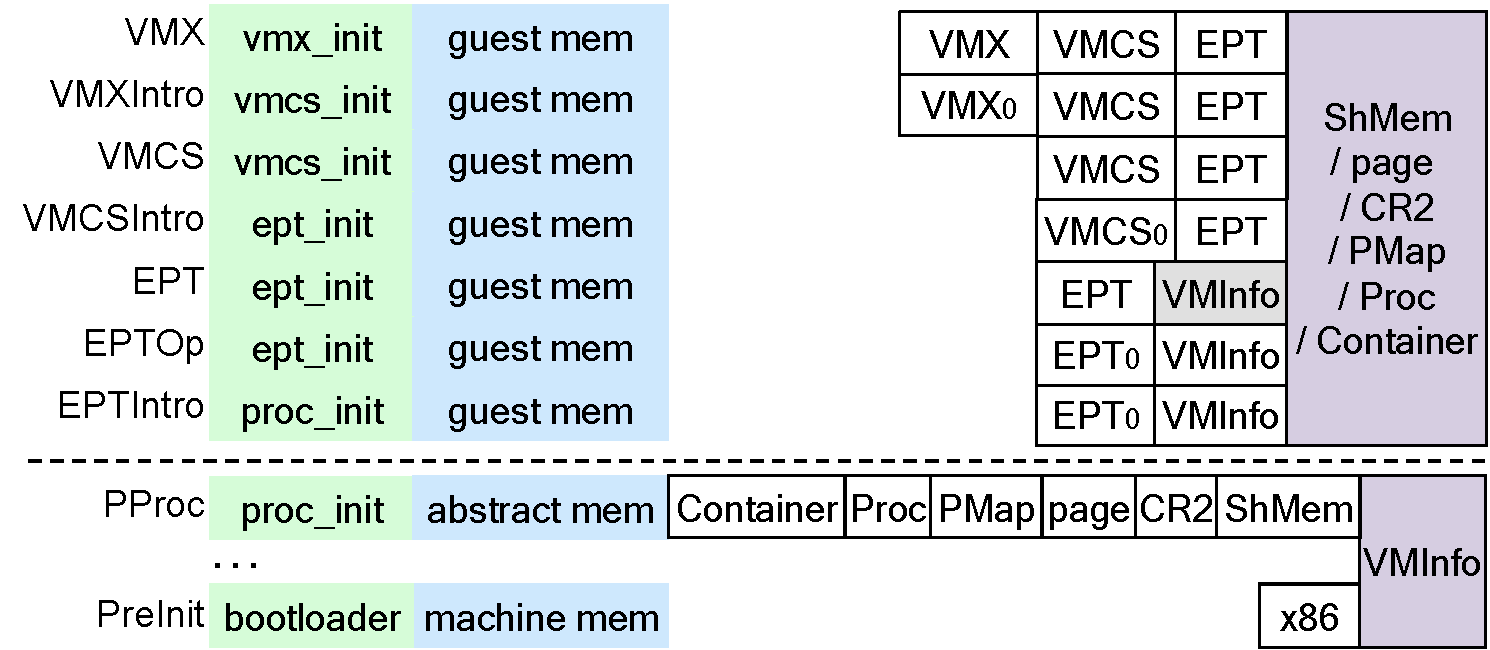
\includegraphics[scale=0.33]{figs/intel_layer}	
%\vspace*{-14pt}
\caption{Layers of virtual machine management}
\label{fig:base:vm:layers}
%\vspace*{-14pt}
\end{figure}

Thanks to the contextual refinement relation we have proved for
\cCTOSbase{}, one can certify user programs using our formal
specifications of system calls. This gives end-to-end proofs on
the behaviors of user programs when they run on \cCTOSbase{}.  
Furthermore, once certified, these processes can safely run in
the privileged ring 0 mode.  We extended \cCTOSbase{} into
\cCTOSringz{} by adding support for spawning ``in-kernel
processes'' that run in the privileged ring 0 mode. 
Ring 0 processes get much
better system call performance by directly calling kernel
functions and avoiding ring switch and interrupt processing. 

The \cCTOSembed{} kernel is intended for embedded settings. To develop
this kernel we started with \cCTOSringz{} and removed the virtual
machine management, the virtual memory management, and some of the
process management layers that are related to user contexts and user
process management.  Thus \cCTOSembed{} only supports ring 0 processes
which run directly inside the physical kernel address space instead of
the user-level paged virtual address space.

Removing plug-ins or layers does not take much effort.
We only need to alter the contextual refinement proof 
at the boundary so we can glue them back together.

\paragraph{Isolation in \cCTOSbase{}}
\label{security}
We have begun exploring the verification of a global security property
on top of \cCTOSbase{}. As a starting point, we proved a basic notion
of isolation between user-level processes running in different virtual
address spaces. This isolation property is composed of two theorems:
one regarding integrity (write protection), and another regarding
confidentiality (read protection, or noninterference).  The statements
of these two theorems are as follows: suppose the top layer abstract
machine takes one step, changing the machine state from $S$ to $S'$,
and let $p$ be the id of the currently-running process (which can be
found in $S$).
\begin{description}
  \item[Integrity:]
If the value at some non-kernel memory location $l$ differs between
$S$ and $S'$, then $l$ belongs to a page that is mapped in the 
virtual address space of $p$.
\item[Confidentiality:]
\label{confidential}
If the step taken
is not a primitive call to an IPC syscall (send, recv, etc.), then the values
of memory in any address space other than $p$'s cannot have an effect on the
result of the step. In other words, if we altered $S$ 
by changing data in a different process's address space, the step would still 
have the same effect on $p$'s address space.
\end{description}

In the future, we plan to provide a more detailed security policy by
describing what can happen to confidentiality when IPC is used.  This
description will be expressed in terms of propagation of security
labels on the IPC data. Note, however, that our framework allows for
security labels to be specified at a purely logical level~--- there is
no need for concrete representation and manipulation of labels at run
time.

Noninterference properties are generally not preserved across
refinement due to nondeterminism. It may therefore seem that the
aforementioned \emph{confidentiality} holds only at the topmost layer,
but not at lower layers. It turns out, however, that our notion of
deep specification is strong enough to preserve
noninterference. Essentially, to give a deep specification to a
nondeterministic semantics, we must first externalize the source of
nondeterminism (e.g., into an oracle). The noninterference property
then becomes parameterized over this source of nondeterminism, which
allows the parameterized property to be preserved across
refinement. This relationship between deep specification,
noninterference, and refinement will be explored comprehensively in
future work.
}



\chapter{Related Work}
\label{chap-rel}

\paragraph{Hoare-style program verification} Hoare logic~\cite{hoare69}
and its modern variants~\cite{reynolds02,boogie05,nanevski06} were
introduced to prove strong (partial or total) correctness properties
of programs annotated with pre- and postconditions. A
total-correctness Hoare triple $[P]C[Q]$ often means a refinement
between the implementation $C$ and the specification $[P,Q]$: given
any state $S$, if the precondition $P(S)$ holds, then the command $C$
can run safely and terminate with a state that satisfies $Q$. Though
not often done, it is also possible to introduce auxiliary/ghost
states to serve as ``abstract states'' and prove that a program
implements a specification via a simulation.
  
Our layer language can be viewed as a novel way of imposing a module
system over Hoare-style program verification. We insist on using
interfaces with deep specifications and we address the ``conflicting
abstract states'' problem mentioned in
Section~\ref{sec:seq:overview}. Traditional program verification does not
always use deep specification (for pre- and post-conditions) so the
module interfaces (\eg, $[P,Q]$) may allow some safe but unwanted
behaviors. Such gap is fine if the goal is to just prove safety (as in
static type-checking), but if we want to prove the strong contextual
correctness property across module boundaries, it is important that
each interface accurately describes the functionality and scope of the
underlying implementation.

In addition to the obvious benefits on compositionality, our layered
approach also enables a new powerful way of combining programming- and
specification languages in a single setting. Each layer interface
enables a new programming language at a specific abstraction level,
which is then used to implement layers at even higher
levels. As we move up the layer hierarchy, our programming language
gets closer and closer to the specification language---it can call
primitives at higher abstraction levels but it still supports
general-purpose programming (\eg, in ClightX).

Interestingly, we did not need to introduce any program logic to
verify our OS kernel code. Instead, we verify it directly using the
ClightX (or LAsm) language semantics (which is already conveniently
parameterized over a layer interface).  In fact, unlike Hoare logic
which shows that a program (\eg, $C$) refines a specification (\eg,
$[P,Q]$), we instead show there is a downward simulation from the
specification to the program. As in CompCert, we found this easier to
prove and we can do this because both our specification and language
semantics are deterministic relative to external events.

\paragraph{Stepwise program refinement}
Dijkstra~\cite{Dijkstra72} proposed to ``realize'' a complex program
by decomposing it into a hierarchy of linearly ordered ``abstract
machines.''  Based on this idea, the PSOS team at SRI~\cite{psos80}
developed the Hierarchical Development Methodology (HDM) and applied
HDM to design and specify an OS using 20 hierarchically organized
modules. HDM was difficult to be rigorously applied in practice,
probably because of the lack of powerful specification and proof
tools. In this paper, we advance the HDM paradigm by using a new formal
layer language to connect multiple layers and by implementing all
certified layers and proofs in a modern proof assistant. We also
pursued decomposition more aggressively since it made our
verification task much easier.

Morgan's refinement calculus~\cite{morgan94} is a formalized approach
to Dijkstra's stepwise refinement. Using this calculus, a high-level
specification can be refined through a series of
correctness-preserving transformations and eventually turned into an
efficient executable. Our work imposes a new layer language to enhance
compositional reasoning. We use ClightX (or
LAsm) and the Coq logic as our ``refinement'' language,
and use a certified layer (with deep specification)
to represent each such correctness-preserving transformation.
All our ClightX and LAsm instances have executable semantics and can be
compiled and linked using our new CompCertX compiler.

\paragraph{Separate compilation for CompCert} Compositional 
compiler correctness is an extremely challenging
problem~\cite{BentonH09,hur12}, especially when it involves an open
compiler with multiple languages~\cite{perconti14}.  In the context of
CompCert, a recent proposal~\cite{beringer14}
aims to tackle the full Clight language but it has not been
fully implemented in the CompCert compiler.  While our CompCertX
compiler proves a stronger correctness theorem for each ClightX layer,
the ClightX language is subtly different from the original
full-featured Clight language. Within each ClightX layer, all locally
allocated memory blocks (\eg, stack frames) cannot be updated by
functions defined in another layer. This means that ClightX does not
support the same general ``stack-allocated data structures'' as in
Clight. This is fine for our OS kernels since they do not allocate any
data structures on stack, but it means that CompCertX can not be
regarded as a full featured separate compiler for CompCert.


As for the concurrency, \citet{stewart15} developed a new compositional extension of the
original CompCert compiler~\cite{compcert} with the goal of providing
thread-safe compilation of concurrent Clight programs.  Their
interaction semantics also treats all calls to synchronization
primitives as external calls. Their compiler does not support a layered
ClightX language as our CompCertX does, so it is unclear how it can
be used to build concurrent layers involving a stack of atomic objects.

%
% Previous work on object invariants have also considered how to specify
% invariants for layered objects. They rely on some auxiliary flags to
% specify when an invariant should hold and when it could fail. 
% 
% Some programming languages (e.g., Spec\#, JML, Eiffel) support rich
% language constructs for specifying contracts, pre- and post conditions
% and object invariants. 
%
% Another class of specification languages are verification intermediate
% languages like Boogie. They make the prescription of verification
% conditions natural and convenient. It contains both mathematical
% and imperative component, but the imperative component is only used
% for verification and it cannot be compiled to generate executable code. 
%
% Dafny is a programming language with classes and datatypes and
% specification constructs for describing intended behaviors. It is
% intended for proving functional correctness.
% 
% Hoare type theory describes a rich dependently typed language whose
% rich types can be used to describe Hoare assertions, but their
% implements relation is still a typechecking relation, not a 
% simulation relation. They do not describe 
%
% Formal specification languages such as TLA, Z, Alloy, and AADL, can
% build sophisticated models and reason about deep properties but they
% are not concerned with connecting to the actual running code.  
%
% Data abstraction is abstraction over shallow specification. The
% representation independence states that the behavior of client
% programs should only depend on the functionality of an abstract
% datatype, not the actual representation type.
%
\paragraph{OS kernel verification} There has been a large body
of recent work on OS kernel verification including
seL4~\cite{klein2009sel4,klein14}, Verve~\cite{hawblitzel10},
and Ironclad~\cite{ironclad14}. None of these works have addressed the
issues on concurrency with fine-grained locking. Very recently,
\citet{xu16} developed a new verification framework based on RGSim
and Feng~{et~al.}'s program logic~\cite{feng08:aim} for reasoning
about interrupts; they have successfully verified many key modules
(in C) in the $\mu$C/OS-II kernel, though so far, they have not proved
any progress properties.

\ignore{
\paragraph{OS kernel verification} The seL4
team~\cite{klein2009sel4} were the first to build a proof of
functional correctness for a realistic microkernel.  The seL4 work is
impressive in that all the proofs were done inside a modern mechanized
proof assistant. They have shown that the behaviors of 7500 lines of
their C code always follow an abstract specification of their
kernel. To make verification easier, they introduced an intermediate
executable specification to hide C specifics. Both their abstract and
executable specifications are ``monolithic'' as they are not divided
into layers to support abstraction among different kernel modules.
These kernel interdependencies led to more complex invariants which
may explain why their effort took 11 person years.

The initial seL4 effort was done completely at the C level so it does
not support many assembly level features such as address translation.
This also made verification of assembly code and kernel initialization
difficult (1200 lines of C and 500 lines of assembly are still
unverified). It is also unclear how to use their verified kernel
to reason about user-level programs since they would be running in a
different address space. Our certified kernels, on the other hand,
directly model assembly-level machines that support all kernel/user
and host/guest programs. Memory access to a user-level address space
must go through a page table, and memory access in a guest virtual
machine must go through a nested page table. We thus had no problem
verifying our kernel initialization or assembly code.


Recently, Sewell {\em et al.}~\cite{sewell13} used translation
validation to build a refinement proof between the
semantics of the seL4 binary (compiled by GCC) and the C source
code. This is an intriguing way of establishing the correctness of a
specific compilation run, as it did not rely on any certified
compiler, but it seems to be more suitable for a fixed code base. 
This might be suitable for seL4 since it is a minimal microkernel
not subject to much modification or extension.

This last point illustrates a key high-level difference between our
two projects. Our compositional approach is developed not just for
building a ``one-off'' lump of a verified microkernel, but instead, it
aims to support advanced development of all kinds of verified kernels.
In particular, we want to apply our layered framework to significantly
enhance the modularity and extensibility of OS kernels.  In place of
the rigid safety conditions used in traditional extension mechanisms
(e.g., that kernel extensions must be
type-safe~\cite{bershad95,hunt07}), our approach will assure both the
safety and semantic {\em correctness} of extensions with respect to
appropriate specifications.
}

\paragraph{Modular verification of low-level code} 
Vaynberg and Shao~\cite{vaynberg12} also used a layered approach to
verify a small virtual memory manager. Their layers are not linearly
ordered; instead, their seven abstract machines form a DAG with
potential upcalls (\ie, calls from a lower layer to upper ones). As a
result, their initialization function (an upcall) was much harder to
verify. Their refinement proofs between layers are insensitive to
termination, from which they can only prove partial correctness but
not the strong contextual correctness property which we prove in our
current work.

Feng {\em et al.}~\cite{feng08:vstte} developed OCAP, an open
framework for linking components verified in different
domain-specific program logics. They verified a
thread library with hardware interrupts and
preemption~\cite{feng08:aim} using a variant of concurrent
separation logic~\cite{ohearn:concur04}. They decomposed the thread
implementation into a sequential layer (with interrupts disabled)
and a concurrent layer (with interrupts enabled).
Chlipala~\cite{BedrockPLDI11} developed Bedrock, an automated
Coq library to support verified low-level programming. All these
systems
are purely sequential, 
and lack the support for concurrency.

\ignore{\paragraph{Certified abstraction layers} \citet{dscal15}
presented the first formal account of certified abstraction layers and
showed how to apply layer-based techniques to build certified system
software. The layer-based approach differs from Hoare-style program
verification~\cite{hoare69,reynolds02,boogie05,nanevski06} in several
significant ways. First, it uses the termination-sensitive forward
simulation techniques~\cite{Lynch95,compcert} and proves a stronger
contextual correctness property rather than simple partial or total
correctness properties (as done for Hoare logics). Second, the overlay
interface of a certified layer object completely removes the internal
concrete memory block (for the object) and replaces it with an
abstract state suitable for reasoning; this abstract state differs
from auxiliary or ghost states (in Hoare logics) because it is
actually used to define the semantics of the overlay abstract machine.
Third, as we move up the abstraction hierarchy by composing more
layers, each layer interface provides a new programming language that gets
closer to the specification language---it can call primitives at
higher abstraction levels while still supporting general-purpose
programming (e.g., in ClightX or LAsm).

Our new formal framework for certified concurrent layers follows the
same layer-based methodologies. Each time we introduce a new concrete
concurrent object implementation, we replace it with an abstract
atomic object in its overlay interface. All shared abstract states are
represented as a single global log, so the semantics of each atomic
method call would need to {\em replay} the entire global log to find
out the return value.  This seemingly ``inefficient'' way of treating
shared atomic objects is actually great for compositional
specification. Indeed, it allows us to apply game-semantic ideas and
define a general semantics that supports parallel layer composition.}

\paragraph{Abstraction for concurrent objects}
\citet{herlihy90} introduced {\em linearizability} as a key technique
for building abstraction over concurrent objects. Developing
concurrent software using a stack of shared atomic objects has since
become the best practices in the system
community~\cite{Herlihy08book,ospp11}. Linearizability is quite
difficult to reason about, and it is not until 20 years later that
\citet{filipovic10} showed that linearizability is actually equivalent
to a termination-insensitive version of the contextual refinement
property. \citet{Gotsman12concur} showed that such equivalence also
holds for concurrent languages with ownership
transfers~\cite{ohearn:concur04}.  \citet{liang13,lili16} showed that
linearizability plus various progress properties~\cite{Herlihy08book}
for concurrent objects are equivalent to various termination-sensitive
versions of the contextual refinement property. These results
convinced us that we should follow \citet{dscal15} and prove
termination-sensitive (contextual) simulation when building certified
concurrent layers as well.

\paragraph{RGSim} Building contextual refinement proofs
for concurrent programs (and program transformations) is challenging.
Liang~{et~al.}~\cite{RGSim,Liang14lics,lili16} developed the
Rely-Guarantee-based Simulation (RGSim) that can support both parallel
composition and also prove contextual refinement of concurrent
objects. Our contextual simulation proofs between two concurrent
layers can be viewed as an instance of RGSim if we extend RGSim with
auxiliary states such as environment contexts and shared logs. This
extension, of course, is the main innovation of our new compositional
layered model. Also, all existing RGSim systems are limited to reasoning
about atomic objects at one layer; their client program context cannot
be the method body of another concurrent object, so they cannot
support the same general vertical layer composition as our work does.

%%%% The following paragraph might be optional %%%%
\citet{lili16} also developed a program logic called LiLi that can
directly prove both the linearizability and starvation-freedom (or
deadlock-freedom) properties. Their ``rely'' conditions are specified
over shared states only, so they cannot express temporal properties. To
prove progress, they have to introduce a separate temporal ``rely''
condition called {\em definite actions}.  This made it difficult to
provide a standalone (total) specification for each lock acquire
method.  Indeed, all examples in their paper are code fragments that
must acquire a lock, then perform critical-section tasks, and then release the
lock. In contrast, our environment context can specify the full
strategies (\ie, both the past and the future behaviors) of all
environment threads and the scheduler, so we can readily impose
temporal invariants over the environment. Within each thread-modular
layer $L[t]$, we can show that each lock acquire primitive (\eg, for
ticket locks) always returns as long as its environment is cooperative
(\eg, always releases its acquired lock), even if $t$ itself may not
be cooperative.
In other words, the termination of $t$'s lock acquire
operation does not depend on whether $t$ itself will release the lock
after first acquiring it.


\paragraph{Treatment of parallel composition}
Most concurrent languages (including those used by RGSim) use a
parallel composition command $(C_1 \| C_2)$ to create and terminate
new threads.  In contrast, we provide thread spawn and join
primitives, and assign every new thread a unique $id$ (\eg, $t$, which
must be a member of the full thread-$id$  domain set $D$). Parallel layer
composition in our work is always done over the whole program $P$ over
all members of $D$. This allows us to reason about the current
thread's behaviors over the environment's full strategies (\ie, both
its past and future behaviors). Even if a thread $t$ is never
created, the semantics for running $P$ over $L[t]$ is still well
defined since it will simply always query its environment context to
construct a global log.

\paragraph{Program logics for shared-memory concurrency}
A large body of new program
logics~\cite{ohearn:concur04,brookes:concur04,SAGL,vafeiadis:marriage,LRG,verifast,gotsman13,Turon13popl,Turon13icfp,nanevski13,nanevski14,sergey15,sergey15pldi,pinto14,iris15,pinto16}
have been developed to support modular verification of shared-memory
concurrent programs. Most of these follow Hoare-style logics so they
do not prove the same strong contextual simulation properties as RGSim
and our layered framework do. Very few of them (\eg,~\cite{pinto16})
can reason about progress properties. Nevertheless, many of these
logics support advanced language features such as high-order functions
and sophisticated non-blocking synchronization, both of which will be
useful for verifying specific concurrent objects within our layered
framework.  Our use of a shared global log and an environment context
resembles the recent work~\cite{sergey15} on using compositional
subjective auxiliary states to represent history traces; the main
difference is again that our environment context can talk about both
past and future behaviors but a history trace can only specify past
behaviors. 


\paragraph{Connection to game semantics} Even though we have used
the game-semantic concepts (\eg, strategies) to describe the
construction of our environment contexts and compositional semantics,
our concurrent machine is still defined using traditional small-step
semantics.  This is in contrast to several past
efforts~\cite{ghica08,nishimura13,rideau11,abramsky99} of modeling
concurrency in the game semantics community where they use games to
define the semantics of a complete language. Modeling higher-order
sequential features as games is great for proving full abstraction,
but it is still unclear how it would affect large-scale program
verification as done in the certified software community.  We do
believe that there are great synergies between the two communities
waiting to be explored and we hope that our current work can serve as
a basis for promoting such interaction.


%\section{Conclusion}
%\label{chap-concl}

\paragraph{Conclusion}
Abstraction layers are key techniques used in building large-scale
computer software and hardware. In this thesis, we have presented a
novel language-based account of sequential and concurrent abstraction layers and shown that they
are particularly suitable for supporting abstraction over deep
specifications, which is essential for compositional verification of
strong correctness properties. We have designed a new layer language
and imposed it on two different core languages (ClightX and LAsm). We
have also built a verified thread-safe compiler from ClightX to LAsm. By
aggressively decomposing each complex abstraction into smaller
abstraction steps, we have successfully developed several certified OS
kernels that prove deeper properties (contextual correctness), contain
smaller trusted computing bases (all code verified at the assembly
level), require significantly less effort, 
\ignore{(6000 lines of C and
assembly code proved in less than 1 person year), }and demonstrate
strong support for extensibility (layers are heavily reused in
different certified kernels).  The
certified concurrent OS kernel we have built supports both fine-grained locking
on multicore machines and blocking synchronization primitives using
thread $\sleep$ and $\wakeup$ primitives. 
We expect that both deep specifications
and certified abstraction layers will become critical technologies and
important building blocks for developing large-scale certified system
infrastructures in the future.
\bibliographystyle{abbrvnat}
\bibliography{os,sec,net,refs}

\end{document}
